% \part{Advanced Quantum Computing}
% \chapter{Hamiltonians}
% \section{Quantum Algorithms for NP-complete Problems}
% We've seen how it's an open question whether quantum computers can solve NP-complete problems in polynomial time. It this turned out to eb possible it would be world-changing. Like, it would be time for a Manhattan Problem to build scalable quantum computers.

% But even if it turns out that quantum computers can't solve NP-complete problems in polynomial time, the question still remains how close can they get. We know from the BBBV theorem that any approach that ignores the structure of NP-complete problems can at most yield the Grover speedup. There have been many papers on the preprint repository arXiv.org that claim to solve NP-complete problems in polynomial time, but do so in ways that violate the BBBV theorem. Virtually all quantum computing papers can be found on arXiv.org , but the site has no peer review so reader beware.

% So to do better than Grover we'd need to exploit problem structure in some way. For example, the Boolean satisfiability we could imagine devising some quantum algorithm that dealt with certain parts of the formula first and worried about other parts later. If we managed to show that any NP-complete problem was in BQP (i.e., solvable in polynomial time by a quantum computer), then by definition all of NP would be in BQP. However, if we are talking about small (polynomial) speedups, then the choice of NP-complete problem might actually matter, because the process of reduction from one NP-complete problem to another might cancel out a speed advantage.

% The Adiabatic Algorithm, proposed by Farhi, Goldstone, Gutman, and Sipser in 2000 is a damous attempt to achieve a quantum speedup for NP-complete problems (conceivably even an exponential speedup) by actually exploiting their structure. It's an extremely important quantum algorithm, but unlike (say) Shor;s or Grover's algorithms, it doesn't come with any rigorous analysis guaranteeing it will run fast in all cases and indeed, we now know that it doesn't. To this day, no one really knows how useful this algorithm will be in practice. It's something that people will eagerly experiment with as soon as they have reliable large-scale quantum computers to test it on!

% For some instances of optimization problems, the adiabatic algorithm might give a huge speed advantage, but for other instances it gives little or no advantage or is even outperformed by classical algorithms. People are trying to figure out for which type of instances the algorithm is most useful.


% To understand the adiabatic algorithm, we first need to back up and familiarize ourselves with a central concepts in quantum mechanics called Hamiltonians.

% In a physics course on quantum mechanics Hamiltonains would be day-one material and we'd only get to quantum computing and information at the very end (if at all). In this course it's exactly the opposite!

% \section{Hamiltonians}
% Recall that unitary matrices are discrete-time linear transformations of quantum states:
% \[
% \ket{\psi}\rightarrow U\ket{\psi}
% \]
% But in physics, time is typically treated as continuous. Rather than viewing the transformation of $\ket{\psi}$ to $U\ket{\psi}$ as a discrete jump, it is viewed as the result of a continuous process causing the state to evolve over some interval of time. Hamiltonians are just the instantaneous time generators of unitary transformations. That is, they're things that give rise to unitary transformations when you ``leave them running" for some period of time. Like density matrices, Hamiltonains are describdd by Hermitian matrices. Unlike density matrices, however, Hamiltonains don't need to be positive semi-definite or to have trace $1$. Physically, Hamiltonians are operators that are used to represent the total energy of the system. (For $H$ to eb Hermitian means that $H=H^{\dagger}$.

% From a physics perspective the central equation of quantum mechanics if Schordinger's equation:
% \[
% \iota \frac{d}{dt}\ket{\psi}=H\ket{\psi}
% \]
% with $H$ being some Hamiltonian. This equation described the evolution of an isolated quantum pure state in continuous time. The fulll version of Schrodinger's equation also includes the so-called Planck's constant $\hbar$, which is needed to convert between units of time and units of energy. But unless we're dealing with actual experimental data (involving real units like meters, seconds, joules and so forth) it's more convenient just to set $\hbar=1$, the convention we'll adopt throughout the rest of the course! For future reference, if it ever comes up, the speed of light $c$ is also $1$.

% Assuming that $H$ is time-independent, we can solve Schrodinger's equation to find that the state after time $t$ is
% \[
% \ket{\psi(t)}=e^{-\iota Ht}\ket{\psi(0)}
% \]
% Schrodinger's equation describes a whole system of linear differential equation one for each coordinate of the vector $\ket{\psi}$ - but we can formally solved it be pretending the matrix $H$ is a scalar.

% \subsection{Matrix Exponentiation}
% We need to back up to address a mathematical point: what does it mean to raise $e$ to the power of a matrix? The ``right" definition turns out to be based on the standard Taylor series for the exponential function
% \[
% e^A=\sum_{k=0}^{\infty} \frac{A^k}{k!}
% \]
% where we now just plug ina. matrix instead of a scalar in order to get a matrix-valued result. Here are some examples:
% \[
% exp(\begin{bmatrix} 0 & 0 \\ 0 & 0 \end{bmatrix})=\begin{bmatrix} 1 & 0 \\ 0 & 1 \end{bmatrix} \quad exp(\begin{bmatrix} 1 & 0 \\ 0 & 0 \end{bmatrix} )= \begin{bmatrix} e & 0 \\ 0 & 1 \end{bmatrix}
% \]
% More generally, for any diagonal matrix we have
% \[
% exp(\begin{bmatrix} 
% \lambda_0 & & \\ & \ddots & \\ & & \lambda_{n-1} \end{bmatrix} = \begin{bmatrix} e^{\lambda_0} & & \\ & \ddots & \\ & & e^{\lambda_{n-1}} \end{bmatrix}
% \]
% In other words, you can exponentiate a diagonal matrix by exponentiating each diagonal term individually.

% The above equation for diagonal matrices might look like a very special case, but for Hermitian matrices it's really all we need! Suppose we're given a Hermitian matrix, $A$. By the Spectral Theorem, we can write $A=UDU^{\dagger}$ where $D$ is diagonal and $U$ is some unitary transformation. To compute $e^A$, we can write
% \begin{align*}
% e^A&=\sum_{k=0}^{\infty} \frac{(UDU^{\dagger})^k}{k!}\\
% &=U\left(\sum_{k=0}^{\infty} \frac{D^k}{k!}\right) U^{\dagger}\\
% &=Ue^DU^{\dagger}
% \end{align*}
% Thus, in order to exponentiate any Hermitian matrix we simply need to diagonalize it first.

% What leverage do we get from $H$ being Hermitian? For what we've said to make sense - and in particular, for it to be consistent with the discrete-time version of QM we've used in the rest of the course - it better be the case that the matrix $e^{-\iota Ht}$ be unitary. Let's now prove this to be true, by using the fact that $H$ is Hermitian.

% Note that if $\ket{v}$ is an eigenvector of $H$ associated with the eigenvalue $\lambda$ then $\ket{v}$ is also an eigenvector of $e^{-\iota Ht}$ with the eigenvalue $e^{-\lambda t}$. So eigenvectors of $H$ give rise to the eigenvectors of the corresponding unitary.

% Now, what about going backwards> Given a unitary $U$, can we always find a Hermitian matrix $H$ such that $U=e^{-\iota Ht}$? yes, this is not hard. First diagonalize $U$ (which we can always do for unitary matrices, agina the spectral theorem) to get $U=VDV^{\dagger}$. We then just need to make matrix logarithm - ike the matrix exponential, this can be defined in terms of the Taylor expansion. Similar to what we found for the matrix exponential , the logarithm of a diagonal matrix can be obtained by taking the logarithm of each entry. For each diagonal element of $D$, $D_{jj}$, we find a $\lambda_j$ such that $D_{jj}=e^{-\iota\lambda_j t}$. Will the set of $\{\lambda_j\}$ that we get by solving this be unique? No, because Euler's formula we can always add $2\pi\iota$ to the exponent and the equation will still hold. We say, for example that
% \[
% \begin{bmatrix} 0 & 0 \\ 0 & 0 \end{bmatrix}
% \]
% is a logarithm to the identity matrix. What else is?
% \[
% \begin{bmatrix} 2\pi\iota & 0 \\ 0 & 2\pi\iota \end{bmatrix},\begin{bmatrix}4\pi\iota & 0 \\ 0 & 6\pi\iota \end{bmatrix},\ldots 
% \]
% Thus, any given unitary can arise from infinitely many different Hamiltonians.

% \subsection{Energy}
% Physicists have a special name for the eigenvalues that you get by diagonalizing a Hamiltonian. They call them energies. Not that they're all real and can therefore be ordered from least to greatest:
% \[
% \begin{bmatrix}
%     \lambda_0 & & \\
%     & \ddots & \\
%     & & \lambda_{n-1}
% \end{bmatrix}
% \]
% with $\lambda_0\leq \lambda_1 \leq \ldots \leq \lambda_{n-1}$. To each energy $\lambda_j$ there corresponds an energy eigenstate $\ket{v_j}$ such that $H\ket{v_j}=\lambda_j\ket{v}$. Why are they called energies? Because they are possible values for the system's energy.

% Quantum mechanics gives us one explanation for why the concept of ``energy" arises in physics. Because unitary matrices arise by exponentiating Hamiltonians and Hamiltonians can be diagonalized and have real eigenvalues.

% If we apply unitary transformation to the energy eigenstate $\ket{v_j}$, we get
% \[
% e^{-\iota Ht}\ket{v_j}=e^{-\iota \lambda_jt}\ket{v_j}
% \]
% meaning that nothing has happened apart from the state picking up a global phase (unorbervable by itself) dependent on the energy. The energy eigenstates  form a complete basis, so wecan write an arbitrary state as a superposition over the energy eigenstates:
% \[
% \ket{\psi}=\alpha_0\ket{v_0}+\ldots+\alpha_{n-1}\ket{v_{n-1}}
% \]
% From this perspective, applying the Hamiltonian $H$ for some amount of $t$ is equivalent to doing
% \[
% e^{-\iota Ht}\ket{\psi}=\alpha_0e^{-\iota \lambda_0t}\ket{v_0}+\ldots+\alpha_{n-1}e^{-\iota \lambda_{n-1}t}\ket{v_{n-1}}
% \]
% This presents a terrifying boring picture of the history of universe? In this picture, all that has ever happened, and all that ever will happen, is that the various energy eigenstates of the universe pickup phases, with each rotation around the unit circuit at a speed proportion to its energy. From the utter lack of interesting activity when we view the world in the energy eigenbasis, we conclude that life is a basis-dependent phenomenon.

% But the above picture is actually extremely useful. For one thing, it suggests that we can simply define energy as the speed at which a quantum state picks up a phase. It's not obvious that this correpsonds to the usual conceptions of energy in physics, but it turns out that it does.

% One thing that's clear from our definitions is that energy is conserved. More formally, the expectation value of the energy in the state $\ket{\psi}$,
% \[
% \bra{\psi}H\ket{\psi}=\sum_j |\alpha_j|^2 \lambda_j
% \]
% stays the same over time.

% We have a special nomenclature for energy eigenstates. The eigenstate $\ket{v_0}$ corresponding to the lowest energy is called the ground state, which we'll see plays an extremely special role in the adiabatic algorithm. The corresponding energy $\lambda_0$ is the ground state energy. The eigenstate $\ket{v_1}$, corresponding to the second-lowest energy, is called the first-excited state. The eigenstate $\ket{v_2}$ is called the second excited state, and so forth. If there's more than one energy eigenvalue equal to $\lambda_0$, then we get what's called a ground state degeneracy. There's no longer unique ground state, but rather a subspace of two or more dimensions in which every state equally minimizes the energy. We can similarly get degnerate excited state if $\lambda_j=\lambda_{j+1}$ for some larger $j$. For the mostpart, though, we'll be able to ignore this.

% The standard game plane for much of moder physics goes like this:

% \begin{itemize}
%     \item 
%     Write down the Hamiltonian $H$ of your system (or some approximation to $H$).
%     \item Diagonalize $H$.
%     \item Extract the energy eigenstates.
%     \item Then, as a first guess, see if your system is just sitting in its ground state doing nothing.
% \end{itemize}

% This initial guess that your system is in the ground state turns out to work very well much of the time. Why are quantum states often found sitting in their ground states? Intuitively, it's because physical systems ``like" to minimize their energy: when lower energy states are available, they ten towards them. The ground state, by definition is the lowest they can go. But since quantum mechanics is time-reversible, how is even possible for a system to be ``attracted" to a certain state? Excellent question? you can thank the Second Law of Thermodynamics and the conservation of energy for this.

% The same question arises in classical physics, which is time-reversible too. If you leave a ball rolling around in a basin and return a while later you probably won't find it in an ``excited state" - i.e. contiuning to roll around. Whatever energy it had in its excited state, it could reach a lower energy by rolling downhill and giving off heat (energy) via friction, eventually coming to a rest. When this happens, the kinetic energy that used to be in the ball dissipates away in the heat.

% In principle it's possible that the reverse could happen: the heat in the basin could coalesce back into the ball and make it spontaneously move. But we essentially never observe that, and the reason comes down to entropy. For all the heat to coalesce back into the motion of the ball would require an absurdly finely-tuned ``conspiracy", in which a massive number of particles synchronize their random motion to impart a kick to the ball. The probability of this synchronized behaviour occurring by chance falls off exponentially with the number of particles. But the reverse process, motion dissipation into heat, requires no similar conspiracy; it only requires that our universe does contain low entropy objects like balls.

% This, in turn, can ultimately be traced back to the low entropy of the universe at the Big Band - something that no one has satisfactorily explained in terms of anything deeper, but we'll be content to leave it there!

% Pretty much exactly the same story works in the quantum case and explains why, when we find quantum systems in nature, they're often sitting in their ground states. If they weren't their interactions with surrounding systems would tend to carry away excess energy until they were. By contrast, all the quantum algorithms and protocols that we've seen in this course are examples of quantum systems that don't just sit in their ground states. Stuff happens, the system evolves. We as people don't just sit in ground states either.

% To give an example of these concepts that the physicists really love, let's talk about the hydrogen atom. In the ground state, a hydrogen atom has its electron sitting in the lowest energy shell (the one closest to the nucleus). The first excited state has the electron in the next shell up (a bit farther away on average from the nucleus). If the atom is in its first excited state, it's easy for it to drop back down to its ground state by emitting a photon. The photon carries away an amount of energy that's exactly equal to the difference between the ground and the first excited energies. Conversely, a hydrogen atom in its ground state can jump up to its first excited state via the electron absorbing a photon. But the later process is not spontaneous; it requires a photon just happening to come by. That's why hydrogen atoms in nature are most often found in their ground states.

% \subsection{Tensor product of Hamiltonians}
% Just like with unitaries we can take tensor product of two or more Hamiltonians to produce a Hamiltonian action on a large system:
% \[
% H=H_0 \otimes H_1
% \]
% We do not, in general have $e^{-\iota (H_0\otimes H_1)}=e^{-\iota H_0}\otimes e^{-\iota H_1}$. However, that equation does hold (up to a global phase) if either $H_0$ or $H_1$ is the identity matrix. In that case, we can think of $H$ acting non-trivially on only one of the two subsystems and trivially on the other (just like with tensor products of unitaries).

% \subsection{Addition of Hamiltonians}
% Our final topic for this chapter is an important operation that we can do with Hamiltonians, but which we couldn't generally do with the unitaries. Namely, we can add them! We can do this simply because the sum of two Hermitian matrices is itself Hermitian, and every Hermitian matrix is a valid Hamiltonian:
% \[
% H=H_0+H_1=H_0^{\dagger}+H_1^{\dagger}=H^{\dagger}
% \]
% What does this mean physically? Intuitively, it just means we've got two things going on at the same time. For example, $H_0$ and $H_1$ could correspond to two different forces acting on our system.


% Building a complicated Hamiltonian by summing local terms could also be seen as somewhat analogous to building a complicated quantum circuit by composing $1$ and $2$-qubit gates.

% To illustrate, at an extremely high level we could write the Hamiltonian for the Standard Model of Elementary particle physics as

% \[
% H_{SM}=H_{Kinetic}+H_{EM}+H_{Strong}+H_{Weak}
% \]
% where $H_{kinetic}$ is the Hamiltonian correpsonding to the Kinetic energy and where $H_{EM}.H_{strong}$ and $H_{weak}$ are the Hamitlonians correspodning to electronmagnetism and to the strong and weak nuclear forces respectively. This isn't exactly right for all sorts of reasons, but is good enough to get across the point.

% The standard model excludes gravity.

% If $A$ and $B$ are matrices is it generally the case that $e^{A+B}=e^Ae^B$? Alas, no. Indeed it's not hard to find a $2\times 2$ counterexample. On the other hand you can check using the Taylor series definition that if $A$ and $B$ commute (that is, $AB=BA$), then $e^{A+B}=e^Ae^B$ does hold.

% We'll care a lot about unitary transformations of the form $e^{-\iota t(A+B)}$, or their counterparts with many more than two Hamiltonians being summed. In particular, we'll need a way to apply these sorts of unitaries efficiently given only the ability to apply $A$ and $B$ by themselves - even if $A$ and $B$ don't happen to commute. Fortunately ther's a trick for this, known as Trotterization. The trick is to use the following approximation:
% \[
% e^{A+B}\approx e^{\epsilon A}e^{\epsilon B}e^{\epsilon A}e^{\epsilon B}\ldots e^{\epsilon A}e^{\epsilon B} (1/\epsilon \text{ times})
% \]
% This basically means that we can achieve the same effect as $A$ and $B$ occurring simultaneously by repeatedly switching between doing a tiny bit of $A$ and a tiny bit of $B$. We won't do it here, but it's possible to prove that the approximation improves as $\epsilon$ decreases, becoming an exact equality int he limit $\epsilon \rightarrow 0$. This is important for the question of how to simulate a real-world quantum system using a quantum computer. Indeed, the straightforward approach is just:
% \begin{itemize}
%     \item Discretize all the degrees of freedom (positions, momenta, etc) that aren't already discrete.
%     \item Write the total Hamiltonian $H$ acting on the system as a sum of ``simple" terms (say, terms that act on only $1$ or $2$ particles as a time).
%     \item Trotterize $H$ in order to approximate it by a product of simple unitary transformations.
% \end{itemize}


% To flesh this out a bit more we ought to say something about what the Hamiltonians of real physical systems tend to look like. Suppose we model the universe as a gigantic lattice of qubits, say in $2$ or $3$ dimension. This is actually exactly the sort of model used to study many condensed matter systems. Suppose too that we only consider interactions between neighboring qubits. In that case, the total Hamiltonian that acts on the qubits can be written
% \[
% H=\sum_j H_+\sum_{j,k}H_{j,k}
% \]
% Here $H_j$ is a Hamitlonian that acts only ont he qubit $j$ and trivially (i.e., as the identity, which has no effect) on all the others, for example:
% \[
% H_0 = \begin{bmatrix} h_1 & h_2 \\ h_3 & h_4 \end{bmatrix} \otimes \begin{bmatrix} 1 & 0 \\ 0 & 1 \end{bmatrix} \otimes \ldots \otimes \begin{bmatrix} 1 & 0 \\ 0 & 1 \end{bmatrix}
% \]
% Meanwhile, for every edge $(j,k)$ in the lattice, $H_{jk}$ is a Hamiltonian that acts non trivially on the neighboring qubits $j$ and $k$ and trivially on all the other qubits, for example:
% \[
% \begin{bmatrix} 0 & & & \\ & 0 & & \\ & & 0 & \\ & & & 1 \end{bmatrix}\otimes \begin{bmatrix} 1 & 0 \\ 0 & 1 \end{bmatrix}^{\otimes n-2}
% \]
% so each qubit ``talks" only to it immediate neighbors in the lattice. Even so, evolving the Hamiltonian over time gives us effects that can propagate arbitrarily far.

% As soon as we've written this, though, we face a puzzle. Won't this lead to faster-than light travel? Indeed, even when $t$ is arbitrarily small, one can check that the unitary matrix $e^{-\iota Ht}$ will generally contain effects of coupling every qubit in the lattice to every other one. Granted, the magnitude of these effects will fall off exponentially with the disctance, but causality demands that there shoudl be literally zero effects propagating across the lattice faster than light.


% So what;s the resolution? basically it's just that the picture we're using comes from non-relativistic quantum mechanics, so it yields a good approximation only if the relevant seeds are small compared to the speed of light. When the speeds are larger, we need to framework of quantum field theory, which does ensure that faster than light influences are exactly zero.

% OK, now we are ready to set things up. Suppose that $H$, a Hamiltonian action on $n$ qubits, is simply the sum of many ``simple" Hamiltonians action on a few qubits each:
% \[
% H=H_0 +\ldots +H_{m-1}
% \]
% Since $H$ is a $2^n \times 2^n$, matrix figuring out its ground state (or ground states) by brute-force diagonalization is extremely time-consuming. This leads to a question: if I know the ground states of the $H_j's$ individually, can I combine them in some simple way to get the ground state of $H$ itself? Alas, the answer is almost certainly ``no". More precisely, we claim that finding the ground state of a Hamiltonian of this form is an NP-hard problem. To prove this we'll show how to take any instance of the famous 3SAT problem and encode it into the ground state problem. Suppose we have a Boolean formula in $n$ variables,
% \[
% \varphi(x_0,\ldots,x_{n-1})=c_0\land \ldots \land c_{m-1}
% \]
% an AND of $m$ clauses, where each clause $c_i$ acts on at most $3$ variables. We can now define an $n$-qubit Hamiltonian $H$ as follows:
% \[
% H=\sum_{i=0}^{m-1}H_i
% \]The term $H_i$ acts on at most $3$ qubits, corresponding to the bits acted on by $c_i$, and as the identity on all the other qubits. It imposes an ``energy penalty" if and only if  the qubits are set in such a way that $c_i$ is violated. For example, we could encode the clause ($v_0 \lor v_1 \lor v_2)$ by the Hamiltonian
% \[
% H=\begin{bmatrix}
%     1 & & & & & & & \\
%      & 0 & & & & & & \\
%      & & 0 & & & & & \\
%      & & & 0 & & & & \\
%      & & & & 0 & & & \\
%      & & & & & 0 & & \\
%      & & & & & & 0 & \\
%      & & & & & & & 0
% \end{bmatrix}
% \]
% This Hamiltonian will yield 0 (no energy penalty) unless all three qubits are set to 0, which corresponds to the case where the clause is not satisfied. It's not hard to see that to minimize the energy for such a Hamiltonian, without loss of generality you just set all the variables classically (superposition states won't help reduce the energy in this case), in whichever way leads to the smallest energy. In other words, you solve 3SAT! In particular, $H$'s ground state energy will be $0$ if $\varphi$ is satisfiable, or some positive value if $\varphi$ is unsatisfiable. So not only is this problem NP-hard, it's NP-hard for reasons that have nothing to do with quantum mechanics. Could this observation somehow let nature solve NP-hard problems in polynomial time?


% \chapter{Trotter based Hamiltonian Simulation}
% Thus, far we have viewed the dynamics of quantum systems from the perspective of unitary transformations: apart from measurement, the only way a quantum state (i.e. a vector of amplitudes) can change is by multiplication with a unitary matrix, for instance a 2-qubit gate tensored with identities on other qubits. but which unitary will actually occur in a given physical system? This is determined by the Hamiltonian of the system, which is the observable $H$ corresponding to the total energy in the system. The expectation value $\braket{\psi|H|\psi}$. Typically,this total energy is the sum of several different terms, corresponding to kinetic energy, potential energy etc. Also typically, it is the sum of many local terms that each act on only a few of the particles (qubits) of the system, for example if all interaction are between pairs of particles. One can think of the Hamiltonian $H$ as describing the physical characteristics of the system. They do determine the evolution of the state in time i.e. the state $\ket{\psi(t)}$ as a function of the time parameter $t$, given an initial state $\ket{\psi(0)}$.

% Trotterization in quantum mechanics is an important theoretical concepts in handling the exponential of non commutative operators. In this communication, we give a mathematical formulation of the trotter Product formula, and apply it to basic examples in which the utility of trotterization is evident.

 
% \begin{proposition}
%     \textit{(Duhamel's principle for Hamiltonian Simulation)} Let $U(t),\tilde{U}(t) \in \mathbb{C}^{N \times N}$
%     satisfy
%     \[ \iota \partial_t U(t)=HU(t), \quad \iota\partial_t \tilde{U}(t) = H\tilde{U}(t) + B(t), \quad U(0)=\tilde{U}(0)=I \]
%     where $H \in \mathbb{C}^{N \times N}$ is a Hermitian matrix and $B(t) \in \mathbb{C}^{N \times N}$ is an arbitrary matrix. Then
%     \[ \tilde{U}(t)=U(t)-\iota\int_0^t U(t-s)B(s)ds \]
%     and
%     \[\|\tilde{U}(t)-U(t)\|\leq \int_0^t\|B(s)\|ds\]
% \end{proposition}
% \begin{proof}
%     Substituting the equation,
%     \[ \tilde{U}(t)=U(t)-\iota\int_0^t U(t-s)B(s)ds \]
%     into the equation,
%     \[ \iota\partial_t \tilde{U}(t) = H\tilde{U}(t)+B(t) \]
%     we see that it satisfies.
%     Now consider a special case where $B(t)=E(t)\tilde{U}(t)$, then
%     \[\tilde{U}(t)=U(t)-\iota \int_0^t U(t-s)E(s)\tilde{U}(s)ds\]
%     Now, taking the norm of the above equation we get:
%     \[\|\tilde{U}(t)-U(t)\|\leq \int_0^t\|E(s)\|ds\]
%     This is a direct analogue o the hybrid argument in the continuous setting.
% \end{proof}

% \section{Simulation of Quantum Systems}
% A useful practical application of quantum circuit model is computation of physical systems. For example, finite element analysis and modelling of bridges to ensure safety while minimizing cost. Cars are made lightweight, structurally sound, attractive, and inexpensive, by using computer aided design. Modern aeronautical engineering depends heavily on computational fluid dynamics simulation for aircraft designs. Nuclear weapons are no longer exploded (for the most part), but rather, tested by exhaustive computational modeling. Examples abound, because of the tremendous practical applications of predictive simulations.

% \subsection{Simulation in action}
% The heart of any simulation is solving differential equations which capture the physical laws governing the dynamical behavior of a system. For example, Newton's Law
% \[
% \frac{d}{dt}\left(m\frac{dx}{dt}\right) = F,
% \]
% Poisson's equation,
% \[
% -\nabla \cdot (k \nabla \vec{u}) = \vec{Q}
% \]
% the electromagnetic vector wave equation,
% \[
% \nabla \cdot \nabla \vec{E}=\epsilon_0 \mu_0 \frac{\partial^2 \vec{E}}{\partial t^2} 
% \]
% and the diffusion equation
% \[
% \vec{\nabla}^2 \psi = \frac{1}{\alpha^2} \frac{\partial \psi}{\partial t}
% \]
% The goal is generally: given an initial state of the system, what is the state at some other time and/or position. Solutions are generally obtained by approximating the state with a digital representation, then discretizing the differential equation in space and time such that an iterative application of a procedure carries the state from the initial to the final conditions. Importantly, the error in this procedure is bounded, and known not to grow faster than some small power of the number of iterations.

% Furthermore, not all dynamical systems be simulated efficiently: generally only those systems which can be described efficiently can be simulated efficiently.

% Simulation of quantum systems by classical computers is possible, but generally only very inefficiently. The dynamical behavior of many simple quantum systems is governed by Schrodinger's equation,
% \[
% \iota \hbar \frac{d}{dt} \ket{\psi} = H \ket{\psi}
% \]
% We will find it convenient to absorb $\hbar$ into $H$, and use this convention for the rest of this section. For a typical Hamiltonian of interest to physicists deal with real particles in space (rather than abstract systems such as qubits, which we have been dealing with) this reduces to
% \[
% \iota \frac{\partial }{\partial t} \psi(x) = \left(-\frac{1}{2m} \frac{\partial^2}{\partial x^2} + V(x)\right) \psi(x)
% \]
% using a convention known as the position representation $\braket{x|\psi}=\psi(x)$. This is also an elliptical equation. So just simulating Schrodinger's equation is not the especial difficulty faced in simulation quantum systems. The key challenge in simulating quantum systems is the exponential number of differential equations which must be solved. For one qubit evolving according to the Schrodinger equation, a system of two differential equations must be solved; for two qubits, four equations; and for $n$ qubits $2^n$ equations. Sometimes' insightful approximations can be made which reduce the effective number of equations involved, thus making classical simulation of the quantum system feasible. However there are many physically interesting quantum systems for which no such approximations are known.

% \begin{example}
%     \textbf{(Exponential complexity growth of quantum systems)} Let $\rho$ be a density matrix describing the state of $n$ qubits. Show that describing $\rho$ requires $4^n-1$ independent real numbers.

%     An operator $\rho$ is the density operator associated to some ensemble $\{p_i,\ket{\psi_i}\}$ if and only if it satisfies the conditions:
%     \begin{enumerate}
%         \item \textbf{(Trace condition)}: $\rho$ has trace equal to one.
%         \item \textbf{(Positivity condition)}$\rho$ is a positive operator.
%     \end{enumerate}
%     Note that $\rho$ will be a $2^n \times 2^n$ dimension matrix. For $\rho$ to be a positive operator it must be Hermitian matrix and for a Hermitian matrix the diagonal elements will always be real. Thus the total number of complex values required is $1+2+3+\ldots + 2^n-1 = \frac{2^n(2^n-1)}{2}=\frac{4^n - 2^n}{2}$.  Hence the number of real values required will be $4^n - 2^n$ (2 for each complex numbers). There are $2^n$ real numbers with the relation that the trace has to be equal to one. Thus, $2^n-1$ independent real numbers for the diagonal. Thus, in total we require $4^n-2^n+2^n-1= 4^n-1$ independent real numbers.
% \end{example}

% The reader with a physics background may appreciate that there are many important quantum systems for which classical simulation is intractable. These include the Hubbard model, a model of interacting fermionic particles with the Hamiltonian
% \[
% H = \sum_{k=1}^n V_0 n_{k\uparrow} n_{k\downarrow} + \sum_{k,j,neighborsm,\sigma} t_0 c^*_{k\sigma}c_{j\sigma}
% \]
% which is useful in the study of superconductivity and magneitsm, the Ising model,
% \[
% H=\sum_{k=1}^n \vec{\sigma}_k \cdot \vec{\sigma}_{k+1}
% \]
% and many others. Solutions to such models give many physical properties such as the dielectric constant, conductivity, and magnetic susceptibility of materials. More sophisticated models such as quantum electrodynamics (QED) and quantum chromodynamics (QCD) can be used to compute constants such as the mass of the proton.

% Quantum computers can efficiently simulate quantum systems for which there is no known efficient classical simulation. Intuitively, this is possible for the same reason any circuit can be constructed from a universal set of quantum gates. Moreover, just as there exist unitary operations which cannot be efficiently approximated, it is possible in principle to imagine quantum systems which cannot be efficiently simulated on a quantum computer. Of course, we believe that such systems aren't actually realized in Nature, otherwise we'd be able to exploit them to do information processing beyond the quantum circuit model.

% \section{Introduction}
% One of the major goals of quantum mechanics is finding solutions, called wavefunctions/eigenfunctions, to the time-independent Schrodinger wave equation. For a given time-independent Hamiltonian operator $\hat{H}$ on a Hilbert space $\mathcal{H}$, the Schrodinger equation is given by
% \[
% \hat{H}\ket{\psi}=E\ket{\psi}
% \]
% where $\ket{\psi}\in\mathcal{H}$ is an eigenfunction and $E\in\mathbb{R}$ is an energy eigenvalue. Alone, this equation only yields the energy values and the stationary states of the physical system. To get the time-dependent eigenvector one needs the unitary operator $U(t)$:
% \[
% U(t)=e^{-\iota\hat{H}t/\hbar}
% \]
% \[
% \ket{\psi(t)}=U(t)\ket{\psi}=e^{-\iota\hat{H}t/\hbar}\ket{\psi}
% \]
% where $\hbar=\frac{h}{2\pi}$ is Planck's reduced constant.

% In practice, it can be hard to compute this operator exponential, so let us focus on the simplest example: When the (finite-dimensional in this case) Hamiltonian operator $\hat{H}$ is given by the diagonal matrix
% \[
% \hat{H}=\begin{pmatrix} E_1 & 0 & \ldots & 0 \\ 0 & E_2 & \ldots & 0 \\ \vdots & \vdots & \ddots & \vdots \\
% 0 & 0 & \ldots & E_n \end{pmatrix}
% \]
% Substituting this in to equation, the eigenfunctions are given by the standard basis
% \[
% \ket{\psi_1} = \begin{pmatrix} 1 \\ 0 \\ \vdots \\ 0 \end{pmatrix}, \ket{\psi_2}=\begin{pmatrix} 0 \\ 1 \\ \vdots \\ 0 \end{pmatrix}, \ldots, \ket{\psi_n}=\begin{pmatrix} 0 \\ 0 \\ \vdots \\ 1 \end{pmatrix}
% \]
% with corresponding eigenvalues $E_1,\ldots,E_n$, respectively. From this, an arbitrary stationary state $\ket{\psi}$ of the entire quantum state is simply a complex $(c_i\in\mathbb{C})$ linear combination:
% \[
% \ket{\psi}=\sum_{i=1}^n c_i\ket{\psi_i}, \sum_{i=1}^n |c_i|^2 =1 
% \]
% This is the time-independent solution. In general $H$ may itself change with $t$, but for simplicity we will only consider here the case where $H$ is time-independent. To get the solution $\ket{\psi(t)}$, we simply need to compute $U(t)$. This is made easy by the fact that the exponential of a diagonal matrix is just the diagonal matrix of element exponentials, Concretely,
% \[
% U(t)=exp\begin{pmatrix} - \iota E_1t/\hbar & 0 & \ldots & 0 \\
% 0 & -\iota E_2 t/\hbar & \ldots & 0 \\ \vdots & \vdots & \ddots & \vdots \\ 0 & 0 & \ldots & -\iota E_nt/\hbar \end{pmatrix}
% \]
% \[
% =\begin{pmatrix} e^{-\iota E_1t/\hbar} & 0 & \ldots & 0 \\
% 0 & e^{-\iota E_2 t/\hbar} & \ldots & 0 \\ \vdots & \vdots & \ddots & \vdots \\ 0 & 0 & \ldots & e^{-\iota E_nt/\hbar} \end{pmatrix}
% \]
% Therefore, the time-dependent state $\ket{\psi(t)}$ is give by
% \begin{align*}
% \ket{\psi(t)}&=U(t)\ket{\psi}\\
% &=\begin{pmatrix} e^{-\iota E_1t/\hbar} & 0 & \ldots & 0 \\
% 0 & e^{-\iota E_2 t/\hbar} & \ldots & 0 \\ \vdots & \vdots & \ddots & \vdots \\ 0 & 0 & \ldots & e^{-\iota E_nt/\hbar} \end{pmatrix}\left(\sum_{i=1}^n c_i\ket{\psi_i}\right)\\
% &=\sum_{i=1}^n c_i e^{-\iota E_it/\hbar}\ket{\psi_i}
% \end{align*}
% This calculation was simple because the Hamiltonian $\hat{H}$ was diagonal, but for the general case we need to use the series definition of exponentiation. Given a (potential infinite dimensional) self-adjoint (Hermitian) operator $S$ defined on $\mathcal{H}$, its exponential is defined by
% \[
% e^S=\sum_{n=0}^{\infty} \frac{S^n}{n!}
% \]
% When $S$ is a finite-dimensional simply diagonalizing the matrix is sufficient to compute $e^S$, and therefore solve the eigenvalue problem. However, when $S$ is infinite dimensional, the problem becomes much more complicated. To help reduce this complexity, we an considering decomposing an operator into a sum.

% If we have another self adjoint operator $T$ defined on $\mathcal{H}$ such that $[S,T]=0(i.e. ST=TS)$, then the exponential of the sum splits:
% \[
% e^{S+T}\xi = e^Se^T \xi \quad \forall \xi \in \mathcal{H}
% \]
% We can actually prove this in a relatively straight-forward manner from the definition of the operator exponential by applying the binomial theorem:
% \begin{align*}
% e^{S+T}&=\sum_{n=0}^{\infty} \frac{(S+T)^n}{n!}\\
% &=\sum_{n=0}^{\infty} \sum_{k=0}^n \frac{1}{n!} ^nC_k S^{n-k}T^k\\
% &=\sum_{n=0}^{\infty} \sum_{k=0}^n \frac{1}{n!} \frac{n!}{(n-k)!k!} S^{n-k}T^k\\
% &=\sum_{n=0}^{\infty}\sum_{k=0}^n \frac{1}{(n-k)!k!}S^{n-k}T^k
% \end{align*}
% With this result, notice that every possible product of $S^m$ with $T^n$ occurs for $m,n \in \mathbb{Z}^+ \cap \{0\}$. Thus, rewrite the sum as follows:
% \begin{align*}
% \sum_{n=0}^{\infty} \sum_{k=0}^n \frac{1}{(n-k)!k!}S^{n-k}T^k &=\sum_{n=0}^{\infty} \sum_{m=0}^{\infty} \frac{1}{m!n!}S^mT^n\\
% &=\left(\sum_{m=0}^{\infty} \frac{1}{m!}S^m\right)\left(\sum_{n=0}^{\infty} \frac{1}{n!} T^n \right)\\
% &=e^S e^T
% \end{align*}
% In the case where $S$ and $T$ do not commute, this argument fails because the Binomial Theorem no longer applies. It seems like there is no way to generalize this argument for the noncommutative case. For example, in the binomial expansion of $(S+T)^3$ with $[S,T]\neq 0$, $STS\neq S^2T$, and so it's impossible to collect terms on the left and right sides overall sum. A somewhat surprising result called the Trotter Product Formula is needed for noncommutative operators, which in a strong sense approximates the above splitting of the exponential. This is what we explore for the remainder of this section.

% Classical simulation begins with the realization that in solving a simple differential equation such as $dy/dt=f(y)$, to first order, it is known that $y(t+\Delta t)\approx y(t)+f(y)\Delta t$. Similarly, the quantum case is concerned with the solution of $\iota \frac{d\ket{\psi}}{dt}=H\ket{\psi}$, which for a time-independent $H$, is just
% \[
% \ket{\psi(t)}=e^{-\iota Ht}\ket{\psi(0)}
% \]
% Since $H$ is usually extremely difficult to exponentiate (it may be sparse, but it is also exponentially large), a good beginning is the first order solution. Note that,
% \begin{align*}
%     \ket{\psi(t_1)} &= e^{-\iota Ht_1}\ket{\psi(0)}\\
%     \ket{\psi(t_2)} &= e^{-\iota Ht_2} \ket{\psi(0)}
% \end{align*}
% Using the fact that $e^{-\iota H(t_2-t_1)}=e^{-\iota Ht_2 + \iota Ht_1}=e^{-\iota Ht_2}e^{\iota Ht_1}$ as decomposition since the matrices $(-\iota Ht_2)(\iota Ht_1)=(\iota Ht_2)(-\iota Ht_1)=H^2t_1t_2$, we can thus write
% \begin{align*}
% \ket{\psi(t_2)}&=e^{-\iota Ht_2}\ket{\psi(0)}\\
% \ket{\psi(t_2)} &= e^{-\iota H(t_2)}e^{\iota Ht_1}e^{-\iota Ht_1}\ket{\psi(t_1)}\\
% \ket{\psi(t_2)}&=e^{-\iota H(t_2-t_1)}e^{-\iota Ht_1}\ket{\psi(0)}\\
% \ket{\psi(t_2)} &=e^{-\iota H(t_2-t_1)}\ket{\psi(t_1)}
% \end{align*}
% Now, putting $t_1=t$ and $t_2=t_1+\Delta t$, we get,
% \[
% \ket{\psi(t+\Delta t)} = e^{-\iota H\Delta t}\ket{\psi(t)} 
% \]
% Thus, $\ket{\psi(t+\Delta t)} \approx (I-\iota H\Delta t)\ket{\psi(t)}$ which roots from the fact that $\ket{\psi(t_2)}=e^{-\iota H (t_2-t_1)} \ket{\psi(t_1)}=e^{-\iota H\Delta t}\ket{\psi(t_1)}$ by putting $t_1=t$ and $t_2=t_1+\Delta t$ and using the fact that (since the matrices $Ht_1$ and $Ht_2$ commute) we can decompose them as $e^{-\iota H(t_2-t_1)}=e^{-\iota Ht_2}e^{\iota Ht_1}$. We get,
% \[
% \ket{\psi(t+\Delta t)} \approx (I-\iota H\Delta t)\ket{\psi(t)}
% \]
% However, such first order solutions are generally not very satisfactory.

% Efficient approximation for the solution to high order, is possible for many classes of Hamiltonians. For example, in most physical systems, the hamiltonian can be written as a sum over many local interactions. Specifically for a system for n particles,
% \[
% H=\sum_{k=1}^L H_k
% \]
% wherever each $H_k$ acts on at most a constant $c$ number of systems, and $L$ is polynomial in $n$. For example, the terms $H_k$ are often just two-body interactions such as $X_iX_j$ and one body Hamiltonians such as $X_i$. Both the Hubbard and Ising models have Hamiltonians of this form. Such locality is quite physically reasonable, and originates in many systems from the fact that the most interactions fall off with increasing distance or difference in energy. There are sometimes additional global symmetry constricts such as particle statistics. The important point is that although $e^{-\iota Ht}$ is difficult to compute, $e^{-\iota H_kt}$ act on a much smaller subsystem, and is straightforward to approximate using quantum circuits. But because $[H_j,H_k]\neq 0$ in general, $e^{-\iota Ht}\neq \prod_k e^{-\iota H_kt}$! How, then can $e^{-\iota H_kt}$ be useful in constructing $e^{-\iota Ht}$.
% Now, we shall also see the extension of this proof where $H$ can be decomposed onto a sum of L Hamiltonians such that they commute. In other words 
% \begin{theorem}
%     Show that $e^{-\iota \hat{H}t}=e^{-\iota \hat{H}_1t}e^{-\iota H_2t}\ldots e^{-\iota \hat{H}_L t}$ if $[\hat{H}_i,\hat{H_j}]=0$ where each $\hat{H}_i=\hat{H}_i^{\dagger}$ i.e. are Hermitian.
% \end{theorem}
% \begin{proof}
%     For any local Hamiltonian $\hat{H}=\sum_{l=1}^L\hat{H}_l$ which consists of $L$ Hermitian terms $\hat{H}_l=\hat{H}_l^{\dagger}$, we are required to prove that the evolution under these Hamiltonian can be decomposed into the product of evolution of local terms if only these terms commute with each other.
%     For
%     \[
%     \hat{H}=\sum_{l=1}^L \hat{H}_l
%     \]
%     we are required to prove that $e^{-\iota \hat{H}t}=e^{-\iota \hat{H}_1 t}e^{-\iota \hat{H}_2t}\ldots e^{-\iota \hat{H}_Lt}$.
%     Without the loss of generality we can prove the above statement for the Hamiltonian consisting of two local terms i.e. $e^{-\iota (\hat{H}_1 +\hat{H}_2 t)}=e^{-\iota \hat{H}_1t}e^{-\iota \hat{H}_2t}$, where $\hat{H}=\hat{H}_1+\hat{H}_2$. Using the formula for Maclaurian series
%     \[
%     e^x=\sum_{n=0}^{\infty}\frac{x^n}{n!}=1+x+\frac{x^2}{2!}+\frac{x^3}{3!}+\ldots
%     \]
%     Thus,
%     \begin{align*}
%     e^{-\iota (\hat{H}_1 +\hat{H}_2 t)}=\sum_{n=0}^{\infty}\frac{(-\iota t\hat{H}_1-\iota t\hat{H}_2)^n}{n!}
%     \end{align*}
%     Then applying the Binomial formula $(x+y)^n=\sum_{k=0}^n \frac{n!}{k!(n-k)!}x^{n-k}y^k$. Note that if $\hat{H}_1\hat{H}_2\neq \hat{H}_2\hat{H}_1$ then in $(\hat{H}_1+\hat{H}_2)^3 \implies \hat{H}_1^2\hat{H}_2 \neq \hat{H}_1\hat{H}_2\hat{H}_1$, i.e. the case when $\hat{H}_1$ and $\hat{H}_2$ do not commute, the Binomial formula is not applicable as reasoned and it is impossible to group them. For our proof since we assume that they commute and using the Binomial formula we get,
%     \[
%     =\sum_{n=0}^{\infty} \frac{1}{n!} \sum_{k=0}^n \frac{n!}{k!(n-k)!} (-\iota t\hat{H}_1)^{n-k}(-\iota t\hat{H}_2)^k
%     \]
%     Upon simplifying we get,
%     \[
%     =\sum_{n=0}^{\infty}\sum_{k=0}^n \frac{(-\iota t\hat{H}_1)^{n-k}}{(n-k)!}\frac{(-\iota t\hat{H}_2)^k}{k!}
%     \]
%     Note that the inner sum for each n are as follows
%     \begin{align*}
%         n=0 &\implies \frac{(-\iota t\hat{H}_1)^0}{0!}\frac{(-\iota t\hat{H}_2)^0}{0!}\\
%         n=1 &\implies \frac{(-\iota t\hat{H}_1)^1}{1!}\frac{(-\iota t\hat{H}_2)^0}{0!}+\frac{(-\iota t \hat{H}_1)^0}{0!}\frac{(-\iota t \hat{H}_2)^1}{1!}\\
%         n=2 &\implies \frac{(-\iota t\hat{H}_1)^2}{2!}\frac{(-\iota t\hat{H}_2)^0}{0!}+\frac{(-\iota t\hat{H}_1)^1}{1!}\frac{(-\iota t\hat{H}_2)^1}{1!}+\frac{(-\iota t \hat{H}_1)^0}{0!}\frac{(-\iota t \hat{H}_2)^2}{2!}\\
%         &\frac{(-\iota t\hat{H}_2)^0}{0!}\left(\frac{(-\iota t \hat{H}_1)^0}{0!} + \frac{(-\iota t \hat{H}_1)^1}{1!}+\frac{(-\iota t \hat{H}_1)^2}{2!}+\ldots \right) +\\
%         &\frac{(-\iota t \hat{H}_1)^1}{1!}\left(\frac{(-\iota t \hat{H}_1)^0}{0!}+\frac{(-\iota t \hat{H}_1)^1}{1!}+\frac{(-\iota t \hat{H}_1)^2}{2!}+\ldots \right) + \\
%         & \frac{(-\iota t \hat{H}_2)^2}{2!}\left(\frac{(-\iota t \hat{H}_1)^0}{0!}+\frac{(-\iota t \hat{H}_1)^1}{1!}+\frac{(-\iota t \hat{H}_1)^2}{2!} +\ldots \right)+\ldots
%     \end{align*}
%     This expression can thus be further simplifies as a multiplication of two independent sums as
%     \[
%     =\sum_{q=0}^{\infty} \sum_{r=0}^{\infty} \frac{(-\iota t\hat{H}_1)^q}{q!}\frac{(-\iota t \hat{H}_2)^r}{r!}=\left(\sum_{q=0}^{\infty} \frac{(-\iota t \hat{H}_1)^q}{q!} \right)\left(\sum_{r=0}^{\infty}\frac{(-\iota t \hat{H}_2)^r}{r!}\right)=e^{-\iota \hat{H}_1t }e^{-\iota \hat{H}_2 t}
%     \]
%     This can be inducitvely extended to all the other terms. Thus, 
%     \[
%     e^{-\iota \hat{H} t}=e^{-\iota \hat{H}_1 t}e^{-\iota \hat{H}_2 t}\ldots e^{-\iota \hat{H}_Lt}
%     \]
%     if $[\hat{H}_i,\hat{H}_j]=0$ for all $i,j$ where each $\hat{H}_i=\hat{H}_i^{\dagger}$ i.e. are Hermitian.
% \end{proof}
% \begin{example}
%     Show that the restriction of $H_k$ to involve at most $c$ particles implies that in the sum,
%     \[
%     H=\sum_{k=1}^L H_k
%     \]
%     $L$ is upper bounded by a polynomial in $n$.

%     If $H_k$ is restricted to involve at most $c$ particles then the number of such Hamiltonians possible will be 
%     \[
%     ^nC_c=\frac{n(n-1)\ldots (n-c+1)}{c!}=\mathcal{O}\left(\frac{n^c}{c!}\right)
%     \]
%     Thus, $L$ will always be upper bounded by a polynomial in $n$ as $\mathcal{O}(n^c)$.
% \end{example}
% \section{Hamiltonian Simulation}
% Quantum systems are described by Hamiltonians where $\hat{H}=\text{Kinetic Energy}+\text{Potential Energy}$. For n qubits $\hat{H}$ is of dimension $2^n \times 2^n$ and $\ket{\psi}$ is of dimension $2^n \times 1$. Thus, the Schrodinger equation
% \[
% \iota \hbar \frac{\partial}{\partial t} \ket{\psi}=\hat{H}(t)\ket{\psi}
% \]
% is exponential to solve on a classical computer. Thus, as Feynman said Simulating Physics with Computers and Quantum computers are Feynman's universal quantum simulators (Seth lloyd). They can calculate evolution of Quantum System Efficiently by doing it in Polynomial time and memory resources in size of target systems. For example, 50 qubits = $2^{50}$ complex numbers. Even if we consider a float 32 bit precision for each part i.e. 32 bits or Real part and 32 bits for Imaginary part for each complex number. We would still have $8 \times 2^{50}$ bytes which is equal to $\approx 9 PB$ of memory equivalent to modern day RAM of supercomputers. 


% Simulating dynamics of Quantum systems such as Ising model, Hubbard Model is one of the practical applications of Quantum Computers. Solutions to these models gives many bulk properties such as dielectric constants, connectivity, magnetic susceptibility of materials and many more. For simulation of atoms, molecules and other biochemical systems we generally require calculation of ground state energy of large systems, study of dynamical behavior of an ensemble of molecules and complex behaviour such as protein folding.

% In areas like quantum chemistry (i.e. ,the study of properties of molecules and their interaction) and material sciences, it is often important to figure out how a quantum system will evolve from some given initial state, for instance a basis state,. It is also very important in chemistry to be able to find out global properties of a given hamiltonian like its lowest energy, a.k.a, ground state energy. Unfortunately this problem seems to be hard to solve (in fact it is so-called QMA hard) even for a quantum computer, even for the special case of 2-local Hamiltonians. This is typically hard to do on a classical computers, since the number of parameters (amplitudes) is exponential in the number of particles. However, a quantum computer is like a universal quantum system, and should be able to efficiently simulate every efficient quantum process, in the same way that a classical Turing machine can efficiently simulate other (classical) physical processes. We will see that it is actually possible to classical simulate quantum computers (and hence quantum systems more generally) with a polynomial amount of space, but out best methods still use an exponential amount of time. If factoring a large integer is a hard problem for classical computers (which is widely believed), then Shor's efficient quantum factoring algorithm implies that it is impossible to simulate a quantum computer in polynomial time on a classical computer. In fact, this was the main reason why Feynman invented quantum computers: a controllable quantum system that can be used to simulate other quantum systems. In order to realize that idea, we need methods to efficiently implement the unitary evolution that is induced by a given Hamiltonian. In other words, we need methods to implement $U=e^{-\iota Ht}$ as a quantum circuit of gates (say, up to some small error $\epsilon$), and to apply this to a given initial state $\ket{\psi}$. This is known as the problem of ``Hamiltonian Simulation". If n-qubit Unitary $\tilde{U}$ (e.g. a quantum circuit with not too many gates) is meant to approximate n-qubit unitary $U$, then we can measure the error by the operator norm of their difference $\|U-\tilde{U}\|=\max_{\psi} \|U\ket{\psi}-\tilde{U}\ket{\psi}\|$. However, we will also see simulation methods that allow some auxiliary qubits, say a of them, which start in the state $\ket{0^a}$ and should end in something close to state $\ket{0^a}$. In this case $\tilde{U}$ acts on more qubits than $U$, so we cannot use the operator norm of their difference, instead we can measure the error on the subspace of $(n+a)$ qubit states where the last a qubits are $\ket{0}$:$\max_{\psi} \|(U\ket{\psi})\ket{0^a} - \tilde{U}(\ket{\psi}\ket{0^a})\|$. This way of measuring error still allows you to analyze a sequence of approximate unitaries using triangle inequality in a way that errors add up at most linearly.

% \subsection{Evolution of a Closed Quantum System}
% Consider the Time-dependent Schrodinger Equation
% \[
% \iota \hbar \frac{\partial}{\partial t}\ket{\psi}=\hat{H}(t)\ket{\psi}
% \]
% where $\hbar$ is the reduced Planck's constant. When the Hamiltonian $\hat{H}$ is constant (does not depend on time) we call it Time independent Hamiltonian and in that case the solution of the Schrodinger's equation is given as
% \[
% \ket{\psi(t)}=e^{-\iota \hat{H}t}\ket{\psi(0)}
% \]
% From this, given a time, we can calculate the state of the system by exponentiating the Hamiltonian. It is generally difficult to exponentiate a Hamiltonian as it may be sparse but exponentially large. Note that $e^{-\iota \hat{H}t}$ is a Unitary matrix.

% \section{The Problem Definition}
% The Hamiltonian simulation problem with a time-independent Hamiltonian, or the Hamiltonian simulation problem for short is the following problem: 
% \begin{definition}Given an initial state $\ket{\psi_0}$ and a Hamiltonian $H$, evaluate the quantum state at time $t$ according to $\ket{\phi(t)}=e^{\iota t H}\ket{\psi_0}$. 
% \end{definition}
% Thus, the goal is to find a sequeunce of computational gates that implement time evolution such that the spectral norm
% \[
% \|U-e^{-\iota \hat{H} t}\|_2\leq \epsilon
% \]
% recall that $\|A\|_2 =\sqrt{\lambda_{max}(A^{\dagger}A)}=\sigma_{max}$.

% Hamiltonian simulation is of immense importance in characterizing quantum dynamics for a diverse range of systems and situations in quantum physics, chemistry and materials science. Simulation of one quantum Hamiltonian by another quantum system was also one of the motivations of Feynman's 1982 proposal for design of quantum computers. We have also seen that Hamiltonian simulation appears as a quantum subroutine in numerous other quantum algorithms such as QPE and its various applications.

% The Hamiltonian simulation problem can also be viewed as a linear ODE:
% \[
% \partial_t\psi(t)=-\iota H\psi(t), \quad \psi(0)=\psi_0
% \]
% However, thanks to the unitary operator $e^{-\iota t H}$ for any $t$, we do not need to store the full history of the quantum states, and can instead focus on the quantum state at time $t$ of interest.

% Following conceptualization of a universal quantum simulator using a Trotter decomposition of time evolution operator $e^{-\iota t H}$, many new quantum algorithms for Hamiltonian simulation have been proposed. This chapter focuses on the Trotter based Hamiltonian simulation methods (also called the product formula).

% \section{Trotter Splitting}
% It is generally difficult to exponentiate a Hamiltonian. In a lot of models, the Hamiltonian can be written as a liner combination of local terms (each term acts only on a part of the total system).
% \[
% \hat{H}=\sum_{l=1}^L \hat{H}_l
% \]
% A k-local Hamiltonian is defined as a Hamiltonian $\hat{H}$ acting on n qubits such that each $\hat{H}_l$ acts non-trivially on atmost k qubits ($k\leq n)$ instead of n qubits. Most Hamiltonains that occur in nature are k-local. Assuming that each local term $\hat{H}_l$ is Hermitian i.e. $\hat{H}_l^{\dagger} = \hat{H}_l$ and can be directly exponentiated. We can present its evolution as a quantum circuit and run it on a quantum computer as 
% \[
% e^{-\iota \hat{H}t}=e^{-\iota \hat{H}_1 t}e^{-\iota \hat{H}_2t}\ldots e^{-\iota \hat{H}_Lt}
% \]
% if and only if they commute $[H_i,H_j]=0$ for all $i,j$. The commuting makes it possible to decompose the evolution of the total Hamiltonian into the product of the local term evolutions. Since each exponent can be represented as a quantum circuit, the Hamiltonian simulation problem is solved for the whole system.

% In general case when local terms do not commute Trotterization is used.
% Consider the Hamiltonian simulation problem $H=H_1+H_2$, where $e^{-\iota H_1 \Delta t}$ and $e^{-\iota H_2 \Delta t}$ can be efficiently computed at least for some $\Delta t$. In general $[H_1,H_2]\neq 0$, and the splitting of the evolution of $H_1,H_2$ needs to be implemented via the Lie product formula
% \[
% e^{-\iota t H}=\lim_{L\rightarrow \infty} \left(e^{- \iota \frac{t}{L}H_1} e^{-\iota \frac{t}{L}H_2}\right)^L
% \]
% When taking L to be a finite number, and let $\Delta t = t/L$, this gives the simplest first order Trotter method with
% \[
% \|e^{-\iota \Delta t H}-e^{-\iota \Delta tH_1} e^{-\iota \Delta tH_2}\|=\mathcal{O}(\Delta t^2)
% \]
% Trotter product formula gives a limit when exponentiation is possible even for not commuting parts. This is represented by many names in the literature as Lie-Product formula, Product formula, Trotter's formula, Trotter product formula, Trotter-Suzuki decomposition, Suzuki-Trotter expansion, Splitting method. It was actually given by Sophus Lie (1875), the later on rediscovered by Hale trotter (1959) and further used by Masuo Suzuki (1976). The formula is
% \[
% e^{A+B}=\lim_{n\rightarrow \infty} \left(e^{\frac{A}{n}} e^{\frac{B}{n}} \right)^n
% \]
% for unbounded linear operators $A,B$. This is called the Lie-Trotter formula.The proof is as follows:
% \begin{proof}
%     Let $A,B$ be Hamiltonian operators and
%     $t\in\mathbb{R}$. Recall
%     \begin{align*}
%         e^x &=\sum_{n=0}^{\infty} \frac{x^n}{n!}=1+x+\frac{x^2}{2!}+\frac{x^3}{3!}+\ldots\\
%         e^{\iota A\frac{t}{n}}&=I+\frac{1}{n}\iota At + \mathcal{O}\left(\frac{1}{n^2}\right)\\
%         \implies e^{\iota At/n}e^{\iota Bt/n}&=\left(I+\frac{\iota At}{n}\right)\left(I+\frac{\iota Bt}{n}\right)+\mathcal{O}\left(\frac{1}{n^2}\right)\\
%         &=I+\frac{\iota At}{n}+\frac{\iota Bt}{n} - \frac{ABt}{n^2}+\mathcal{O}\left(\frac{1}{n^2}\right)\\
%         &=I+\frac{1}{n}\iota(A+B)t+\mathcal{O}\left(\frac{1}{n^2}\right)\\
%         \implies \left(e^{\iota At/n}e^{\iota Bt/n}\right)^n &=I+\sum_{k=1}^n \frac{n!}{(n-k)!k!} \frac{1}{n^k}[\iota (A+B)t]^k+\mathcal{O}\left(\frac{1}{n}\right)
%     \end{align*}
%     Using the Binomial formula for $(x+y)^n=\sum_{k=0}^n \frac{n!}{(n-k)!k!}x^{n-k}y^k$
%     \[
%         =\sum_{k=0}^n=\frac{n!}{(n-k)!k!}\frac{1}{n^k}(\iota (A+B)t)^k
%     \]
%     Now,
%     \begin{align*}
%     \lim_{n\rightarrow \infty} \frac{n!}{(n-k)!k!}\frac{1}{n^k} &=\lim_{n\rightarrow \infty}\frac{1}{k!}\frac{n(n-1)\ldots (n-k-1)}{n^k}\\
%     &=\lim_{n\rightarrow \infty} \frac{1}{k!}\left(1-\frac{1}{n}\right)\left(1-\frac{2}{n}\right)\ldots \left(1-\frac{k-1}{n}\right)\\
%     &\approx \frac{1}{k!}\left(1+\mathcal{O}\left(\frac{1}{n}\right)\right)\\
%     \end{align*}
%     Hence, upon substituting the result in the given equation, we get,
%     \begin{align*}
%     \lim_{n\rightarrow \infty} (e^{\iota At/n}e^{\iota Bt/n})^n&=\lim_{n\rightarrow \infty}\sum_{k=0}^n \frac{1}{k!} \left(1+\mathcal{O}\left(\frac{1}{n}\right)\right)(\iota (A+B)t)^k + \mathcal{O}\left(\frac{1}{n}\right)\\
%     \lim_{n\rightarrow \infty} (e^{\iota At/n}e^{\iota Bt/n})^n&=\sum_{k=0}^n \frac{(\iota(A+B)t)^k}{k!}\\
%     \lim_{n\rightarrow \infty} \left(e^{\iota At/n} e^{\iota Bt/n}\right)^n &=e^{\iota (A+B)t}
%     \end{align*}
% \end{proof}
% Modifications of the trotter formula provide the methods by which higher order approximations can be derived for performing quantum simulations. For example, using similar reasoning to the proof above, it can be shown that
% \[
% e^{\iota (A+B)\Delta t}=e^{\iota A\Delta t}e^{\iota B\Delta t} + \mathcal{O}(\Delta t^2)
% \]
% Similarly, 
% \[
% e^{\iota (A+B)\Delta t}=e^{\iota A\Delta t/2}e^{\iota B \Delta t}e^{\iota A \Delta t/2} + \mathcal{O}(\Delta t^3)
% \]
% \begin{example}
% Let $H = \sum_k^L H_k$, and define
% \[
% U_{\Delta t}=\left(e^{-\iota H_1\Delta t}e^{-\iota H_2\Delta t}\ldots e^{-\iota H_L\Delta t}\right)\left(e^{-\iota H_L\Delta t}e^{-\iota H_{L-1}\Delta t}\ldots e^{-\iota H_1\Delta t}\right)
% \]
% \begin{enumerate}[label=(\alph*)]
%     \item Prove that $U_{\Delta t}=e^{-2\iota H\Delta t} + \mathcal{O}(\Delta t^3)$
%     \item Use the results in Box 4.1 to prove that for a positive integer $m$,
%     \[
%     E(U_{\Delta t}^m,e^{-2m\iota H\Delta t}) \leq m\alpha\Delta t^3
%     \]
% \end{enumerate}
% \begin{enumerate}[label=(\alph*)]
%     \item Using the following formula,
% \[
% e^{\iota (A+B)\Delta t} = e^{\iota A\Delta t/2}e^{\iota B\Delta t}e^{\iota A\Delta t/2} + \mathcal{O}(\Delta t^3)
% \]
% We can then simplify the above expression as follows:
% \begin{align*}
%     U_{\Delta t}&=\left(e^{-\iota H_1\Delta t}e^{-\iota H_2\Delta t}\ldots e^{-\iota H_L\Delta t}\right)\left(e^{-\iota H_L\Delta t}e^{-\iota H_{L-1}\Delta t}\ldots e^{-\iota H_1\Delta t}\right)\\
%     &=\left(e^{-\iota H_1\Delta t}e^{-\iota H_2\Delta t}\ldots e^{-2\iota H_L\Delta t}e^{-\iota H_{L-1}\Delta t}\ldots e^{-\iota H_1\Delta t}\right)
% \end{align*}
% Because $[H_L,H_L]=0$, thus we can write $e^{-\iota H_L\Delta t}e^{-\iota H_L\Delta t}=e^{-2\iota H_L\Delta t}$. Now applying the formula for terms, $e^{-2\iota H_{L-1}\Delta t/2}e^{-2\iota H_{L}\Delta t}e^{-2\iota H_{L-1}\Delta t/2} = e^{2\iota (H_{L-1} + H_L)\Delta t} + \mathcal{O}(\Delta t^3)$, thus using this formula recursively, say for a term 
% \[
% e^{-2\iota H_j\Delta t/2}e^{-2\iota \sum_{k=j+1}^L H_k\Delta t} e^{-2\iota H_j\Delta t/2} = e^{-2\iota \sum_{k=j}^L H_k \Delta t} + \mathcal{O}(\Delta t^3)
% \]
% thus, we get,
% \begin{align*}
%     U_{\Delta t} &=e^{-2\iota H_1\Delta t/2}e^{-2\iota \sum_{k=2}^L H_k \Delta t} e^{-2\iota H_1\Delta t/2} +\mathcal{O}(\Delta t^3)\\
%     &=e^{-2\iota \sum_{k=1}^L H_k \Delta t} + \mathcal{O}(\Delta t^3)\\
%     &=e^{-2\iota H\Delta t} + \mathcal{O}(\Delta t^3)
% \end{align*}
% Hence proved.
% \item Using the result from Box 4.1 as stated below
% \[
% E(U_mU_{m-1}\ldots U_1, V_m V_{m-1}\ldots V_1) \leq \sum_{j=1}^m E(U_j,V_J)
% \]
% Thus,
% \[
% E(U_{\Delta t}^m ,e^{-2m\iota H\Delta t}) = E(U_{\Delta t}U_{\Delta t}\ldots U_{\Delta t},e^{-2\iota H\Delta t}e^{-2\iota H\Delta t}\ldots e^{-2\iota H\Delta t})
% \]
% can be simplified as follows
% \begin{align*}
%     E(U_{\Delta t}U_{\Delta t}\ldots U_{\Delta t},e^{-2\iota H\Delta t}e^{-2\iota H\Delta t}\ldots e^{-2\iota H\Delta t})&\leq \sum_{j=1}^m E(U_{\Delta t},e^{-2\iota H\Delta t})\\
%     &\leq \sum_{j=1}^m \max_{\ket{\psi}} \|(U_{\Delta t} - e^{-2\iota H\Delta t})\ket{\psi}\| \\
%     &\leq \sum_{j=1}^m \max_{\ket{\psi}}\|\mathcal{O}(\Delta t^3)\ket{\psi}\|\\
%     &\leq m\alpha \Delta t^3
% \end{align*}
% Here we have used the fact as derived in part (a) that $E(U_{\Delta t},e^{-2\iota H\Delta t}) =\alpha \Delta t^3$. For some constant $\alpha$ because of the term $\mathcal{O}(\Delta t^3)$, we thus get the following result
% \[
% E(U_{\Delta t}^m,e^{-2\iota mH\Delta t}) \leq m\alpha\Delta t^3
% \]
% \end{enumerate}
% Hence, proved.
% \end{example}
% We can thus apply this formula to the k-local Hamiltonians even when they do not commute with each other.
% \[
% e^{-\iota \sum_{l=1}^L \hat{H}_l t}=\lim_{n\rightarrow \infty}\left( \prod_{e=1}^L e^{-\iota \hat{H}_l \frac{t}{n}}\right)^n
% \]
% Note that this formula involves infinity so we need to truncate the series when implementing this formula on a quantum computer. It is this truncation that introduces error in the simulation
% \[
% e^{-\iota \sum_{l=1}^L \hat{H}_l t}\approx \left(\prod_{l=1}^L e^{-\iota \hat{H}_l\frac{t}{n}}\right)^n
% \]
% This truncation and application of Suzuki-trotter formula to Hamiltonian simulation problem is known as Trotterization and its widely used to simulate non-commuting Hamiltonians on Quantum Computers. When the local terms of the hamiltonians commute the identity is exact.
% Therefore to perform Hamiltonian simulation to time t, the error is
% \[
% \|e^{-\iota t H}-\left(e^{-\iota \frac{t}{L}H_1} e^{-\iota \frac{t}{L}H_2}\right)^L\| = \mathcal{O}(\Delta t^2L)=\mathcal{O}\left(\frac{t^2}{L}\right)
% \]
% Note that the error term is actually $O(\|H_1\|\|H_2\|t^2/n)$.
% So to reach precision $\epsilon$ in the operator norm, we need
% \[
% L=\mathcal{O}(t^2\epsilon^{-1})
% \]
% Thus, the number of trotter steps is $L$, and is chosen such that the simulation error reaches the desired value.
% This can be improved to the second order Trotter method (also called the symmetric trotter splitting or Strang splitting)
% \begin{align*}
% \|e^{-\iota \Delta t H}-e^{-\iota \Delta t/2 H_2}e^{-\iota \Delta tH_1}e^{-\iota \Delta t/2H_2}=\|=\mathcal{O}(\Delta t^3)
% \end{align*}
% Following a similar analysis to the first order method, we find that to reach precision $\epsilon$ we need
% \[
% L=\mathcal{O}(t^{\frac{3}{2}}\epsilon^{-1/2})
% \]
% Higher order Trotter methods are also available, such as the p-th order Suzuki formula. The local truncation error is $(\Delta t)^{p+1}$. therefore to reach precision $\epsilon$, we need
% \[
% L=\mathcal{O}(t^{\frac{p+1}{p}}\epsilon^{-1/p})
% \]
% This is often written as $L=\mathcal{O}(t^{1+o(1)}\epsilon^{-o(1)})$  as $p\rightarrow \infty$.
% Below given is the algorithm for simulating the Quantum Systems, along with an explicit example of simulation the one-dimensional non-relativistic Schrodinger equation.
% \begin{algorithm}
%     \caption{Quantum Simulation}
%     \begin{algorithmic}[1]
%     \State \textbf{Input:} A Hamiltonain $H=\sum_k H_k$ acting on an $N$-dimensional system, where each $H_k$ acts on a small subsystem of size independent of $N$, (2) An initial state $\ket{\psi_0}$, of the system at $t=0$. (3) A positive, non-zero accuracy $\delta$, and (3) A time $t_f$ at which the evolved state is desired.
%     \State \textbf{Output:} A state $\ket{\tilde{\psi}(t_f)}$ such that $|\bra{\tilde{\psi}(t_f)}e^{-\iota Ht_f}\ket{\psi_0}|^2 \geq 1-\delta$
%     \State \textbf{Runtime: } $\mathcal{O}(poly(1/\delta))$
%     \State \textbf{Procedure:} 
%    Choose a representation such that the state $\ket{\tilde{\psi}}$ of $n=poly(\log N)$ qubits approximates the system and the operators $e^{-\iota H_k\Delta t}$ have efficient quantum circuit approximation. Select an approximation method and $\Delta t$ such that the expected error is acceptable (and $j\Delta t=t_f$ for an integer $j$), construct the corresponding quantum circuit $U_{\Delta t}$ for the iterative step and do:
%    \begin{enumerate}
%        \item \textbf{Initialize State: } $\ket{\tilde{\psi}_0} \leftarrow \ket{\psi_0}; \quad j=0$
%        \item \textbf{Iterative Update:} $\rightarrow \ket{\tilde{\psi}_{j+1}} = U_{\Delta t}\ket{\tilde{\psi}_j}$
%        \item \textbf{Loop:} $\rightarrow j=j+1$; goto 2 until $j\Delta t \geq t_f$
%        \item \textbf{Final Result:} $\rightarrow \ket{\tilde{\psi}(t_f}=\ket{\tilde{\psi}_j}$
%    \end{enumerate}
%     \end{algorithmic}
% \end{algorithm}

% \begin{example}
% Say Hamiltonian $\hat{H}$ we want to simulate is a sum of two Pauli matrices $\hat{H}=\hat{X}+\hat{Z}$ which acts on a single qubit. Note that it is small enough to do an exact simulation and compare it with a simulation using trotterization for different no. of Trotter steps. The matrix is simultaneous rotation around X and Z axis of the Bloch sphere. Recall that because the Pauli X and Pauli Z do not commute i.e. $[X,Z]=2\iota Y$, thus $e^{-\iota Ht}=e^{-\iota (X+Z)t}\neq e^{-\iota Xt}e^{-\iota Zt}$. Thus, we use trotterization. Say we use first-order trotterization as follows:
% \[
% e^{-\iota Ht}=\left(e^{-\iota X\frac{t}{n}}e^{-\iota Z \frac{t}{n}}\right)^n
% \]
% We, thus evolve the Hamiltonian repeatedly by switching between evolving $X$ and $Z$ each for a small period of time. Thus, the next step is to represent each product in Trotter's formula as a quantum circuit. In this case it is simple because evolution can be represented exactly using Rotations around $X$ and $Z$ axis. Recall,
% \[
% e^{-\iota \frac{\theta}{2} X}=R_x(\theta)=\begin{pmatrix} \cos (\theta/2) & -\iota \sin(\theta/2) \\ -\iota \sin(\theta/2) & \cos (\theta/2) \end{pmatrix}
% \]
% and
% \[
% e^{-\iota \frac{\theta}{2} Z}=R_Z(\theta)=\begin{pmatrix} e^{-\iota \frac{\theta}{2}} & 0 \\ 0 & e^{\iota \frac{\theta}{2}} \end{pmatrix}
% \]
% Rotation angle then encodes the evolution. Putting $\theta=\frac{2t}{n}$, we get,
% \[
% R_x\left(\frac{2t}{n}\right)=e^{-\iota \frac{t}{n} X}=\begin{pmatrix} \cos (\frac{t}{n}) & -\iota \sin (\frac{t}{n}) \\ -\iota \sin(\frac{t}{n}) & \cos (\frac{t}{n}) \end{pmatrix}; \quad R_Z\left(\frac{2t}{n}\right) =e^{-\iota \frac{t}{n} Z}=\begin{pmatrix} e^{-\iota \frac{t}{n}} & 0 \\ 0 & e^{-\iota \frac{t}{n}} \end{pmatrix}
% \]
% The more the terms are commuting between each other, the more precise the simulation is. The 1st order formula is good for short time intervals. Note that we did not require any ancilla bits.
% \end{example}

% \begin{example}
%     \textbf{(Baker-Campbell-Hausdorf formula)} Prove that
%     \[
%     e^{(A+B)\Delta t}=e^{A\Delta t}e^{B\Delta t} e^{-\frac{1}{2}[A,B]\Delta t^2} + \mathcal{O}(\Delta t^3)
%     \]
%     and also prove that $e^{\iota (A+B)\Delta t}=e^{\iota A\Delta t}e^{\iota B\Delta t} + \mathcal{O}(\Delta t^2)$ and
%     $e^{\iota (A+B)\Delta t}=e^{\iota A\Delta t/2}e^{\iota B\Delta t}e^{\iota A\Delta t/2} + \mathcal{O}(\Delta t^3)$.

%     We will begin with proving $e^{\iota (A+B)\Delta t}=e^{\iota A\Delta t}e^{\iota B\Delta t} + \mathcal{O}(\Delta t^2)$. Recall, from the trotter formula proof that
%     \[
%     e^{\iota At/n}e^{\iota Bt/n} =I+\frac{1}{n}\iota (A+B)t + \mathcal{O}\left(\frac{1}{n^2}\right)
%     \]
%     Putting $t=n\Delta t \implies n = \frac{t}{\Delta t}$, we get,
%     \begin{align*}
%     e^{\iota A\Delta t}e^{\iota B\Delta t}&=I+\iota (A+B)\Delta t + \mathcal{O}(\Delta t^2)\\
%     e^{\iota A\Delta t}e^{\iota B\Delta t}-\mathcal{O}(\Delta t^2)&=e^{\iota (A+B)\Delta t}\\
%     \implies e^{\iota (A+B)\Delta t} &= e^{\iota A\Delta t}e^{\iota B \Delta t} + \mathcal{O}(\Delta t^2)
%     \end{align*}
%     Now proving $e^{\iota (A+B)\Delta t}=e^{\iota A\Delta t/2}e^{\iota B\Delta t}e^{\iota A\Delta t/2} + \mathcal{O}(\Delta t^3)$
%     \begin{align*}
%         e^{\iota A\Delta t/2}e^{\iota B\Delta t}e^{\iota A\Delta t/2} &= \left(I+\iota A\Delta t/2 + \frac{(\iota A\Delta t/2)^2}{2!}\right)\left(I+\iota B\Delta t + \frac{(\iota B\Delta t)^2}{2!}\right)\\
%         &\quad \left(I+\iota A\Delta t/2 + \frac{(\iota A\Delta t/2)^2}{2!}\right)\\
%         &=I+\iota (A+B)\Delta t + \frac{(\iota (A+B)\Delta t)^2}{2!} + \mathcal{O}(\Delta t^3)\\
%         \implies e^{\iota (A+B)\Delta t} &=e^{\iota A\Delta t/2}e^{\iota B\Delta t}e^{\iota A\Delta t/2} + \mathcal{O}(\Delta t^3)
%     \end{align*}
%     Now proving the baker-Campbell-Hausdorf formula,
%     \begin{align*}
%         e^{A\Delta t}e^{B\Delta t}e^{-\frac{AB-BA}{2}\Delta t^2} &=\left(I+A\Delta t+\frac{(A\Delta t)^2}{2}\right)\left(I+B\Delta t+\frac{(B\Delta t)^2}{2}\right) \left(I-\frac{AB-BA}{2}\Delta t^2\right)\\
%         &=I+A\Delta t+B\Delta t+\frac{(A\Delta t)^2}{2}+\frac{(B\Delta t)^2}{2} +AB\Delta t^2 -\frac{AB\Delta t^2}{2}\\
%         &+\frac{BA\Delta t^2}{2} +\mathcal{O}(\Delta t^3)\\
%         &=I+(A+B)\Delta t+\frac{A^2+B^2 +AB + BA}{2}\Delta t^2 +\mathcal{O}(\Delta t^3)\\
%         &=I+(A+B)\Delta t +(A+B)^2\frac{\Delta t^2}{2} + \mathcal{O}(\Delta t^3)\\
%         \implies e^{(A+B)\Delta t}&=e^{A\Delta t}e^{B\Delta t}e^{-\frac{AB-BA}{2}\Delta t^2} + \mathcal{O}(\Delta t^3)
%     \end{align*}
% \end{example}
% \begin{example}
%     (Simulating transverse field Ising model). For the one dimensional transverse filed Ising model (TFIM) with nearest neighbor interaction, wince all Pauli-$Z_i$ operators commute, we have
%     \[
%     e^{-\iota tH_1}:=e^{\iota t}\sum_{i=1}^{n-1} Z_iZ_{i+1} = \Pi_{i=1}^{n-1} e^{\iota t Z_i Z_{i+1}}
%     \]
%     Each $e^{\iota t Z_i Z_{i+1}}$ is a rotation involving only the qubits $i,j$, and the splitting has no error. Similarly
%     \[
%     e^{-\iota t H_2}:=e^{d\sum_)iX_i}= \Pi_i e^{\iota t g X_i}
%     \]
%     and each $e^{\iota t g X_i}$ can be implemented independently without error.
% \end{example}



% \begin{example}
%     (Particle in a Potential). Let $H=-\Delta_r + V(\mathbf{r})=H_1+H_2$ be the Hamiltonian of a particle in a potential field $V(\mathbf{r})$, where $\mathbf{r} \in \Omega = [0,1]^d$ with periodic boundary conditions. After discretization using Fourier modes, $e^{\iota H_1 t}$ can be efficiently performed by diagonalizing $H_1$ in the Fourier space, and $e^{\iota H_2t}$ can be efficiently performed since $V(\mathbf{r})$ is diagonal in the real space.
% \end{example}
% \section{Evolution of Hamiltonian formed by Pauli Operators: Quantum circuits and exact simulation}
% Evolution generated by some non-local Hamiltonians can be simulated exactly. Such a possibility occurs when a hamiltonian consists of Tensor product of Pauli operators. Examples of such Hamiltonians are $\hat{H}=\hat{X},\hat{H}=\hat{Z}_1\otimes \hat{Z}_2, \hat{H}=\hat{X}_1\otimes \hat{Y}_2\otimes \hat{Z}_3$. In total any Hamiltonian of the form:
% \[
% \hat{H}=\otimes_{k=1}^n \sigma_{\alpha k}^k
% \]
% We will now see how to construct a quantum circuit a Quantum circuit to simulate a Hamiltonian consists of an arbitrary tensor product of Pauli operators.
% \subsection{One-qubit Hamiltonians}
% In other words, when the Hamiltonians is formed by one of the Pauli operators ($\hat{H}=\{X,Y,Z,I\})$. In this case, the evolution operator is just the corresponding rotation Operators.
% \[
% U=e^{-\iota \hat{H}t}
% \]
% \begin{align*}
%     R_x(\theta)&=e^{-\iota \frac{\theta}{2}\hat{X}}=\cos \frac{\theta}{2} \hat{I}-\iota \sin \frac{\theta}{2}\hat{Y}=\begin{pmatrix} \cos \frac{\theta}{2} & -\iota \sin \frac{\theta}{2} \\ -\iota \sin \frac{\theta}{2} & \cos \frac{\theta}{2} \end{pmatrix}\\
%     R_Y(\theta)&=e^{-\iota \frac{\theta}{2}\hat{Y}}=\cos \frac{\theta}{2} \hat{I}- \iota \sin \frac{\theta}{2}\hat{Y}=\begin{pmatrix} \cos \frac{\theta}{2} & \sin \frac{\theta}{2} \\ \sin \frac{\theta}{2} & \cos \frac{\theta}{2} \end{pmatrix}\\
%     R_Z(\theta)&=e^{-\iota \frac{\theta}{2}\hat{Z}}=\cos \frac{\theta}{2} \hat{I}-\iota \sin \frac{\theta}{2}\hat{Z}=\begin{pmatrix} e^{-\iota \frac{\theta}{2}} & 0 \\ 0 & e^{\iota \frac{\theta}{2}} \end{pmatrix}
% \end{align*}
% \subsection{Two-qubit Hamiltonians}
% Now consider the situation when the Hamiltonian consists of Pauli operators applied to two qubits. Say $\hat{H}=\hat{Z}_1 \otimes \hat{Z}_2$. Here, the subscript denotes the qubit it acts on. The Hamiltonian is as follows:
% \[
% \hat{Z}_1\otimes \hat{Z}_2=\begin{pmatrix} 1 & 0 \\ 0 & -1 \end{pmatrix} \otimes \begin{pmatrix} 1 & 0 \\ 0 & -1 \end{pmatrix}=\begin{pmatrix} 1 & 0 & 0 & 0 \\ 0 & -1 & 0 & 0 \\ 0 & 0 & 1 & 0 \\ 0 & 0 & 0 & -1 \end{pmatrix}
% \]
% Note that the square of this matrix is an Identity matrix. Therefore, to calculate the evolution operator of a given Hamiltonian we can use the formula for the decomposition of the matrix exponential.
% \[
% U=e^{-\iota (\hat{Z}_1\otimes \hat{Z}_2) t}=\cos t \hat{I}_1\otimes \hat{I}_2 -\iota \sin t \hat{Z}_1 \otimes \hat{Z}_2
% \]
% \[
% =\begin{pmatrix} \cos t -\iota \sin t & 0 & 0 & 0 \\ 0& \cos t+\iota \sin t & 0 & 0 \\ 0 & 0 & \cos t+\iota \sin t & 0 \\ 0 & 0 & 0 & \cos t-\iota \sin t \end{pmatrix}
% \]
% using the exponential notation of the colex number, we get,
% \[
% =\begin{pmatrix} e^{-\iota t} & 0& 0 & 0 \\ 0& e^{\iota t} & 0 & 0 \\ 0& 0 & e^{\iota t} & 0 \\ 0 & 0 & 0 & e^{-\iota t} \end{pmatrix}
% \]
% \[
% \hat{R}_{ZZ}(\theta)=e^{-\iota \frac{\theta}{2} \hat{Z}_1 \otimes \hat{Z}_2}=\begin{pmatrix} e^{-\iota \frac{\theta}{2}} & 0 & 0 & 0 \\ 0 & e^{\iota \frac{\theta}{2}} & 0 & 0 \\ 0 & 0 & e^{\iota \frac{\theta}{2}} & 0 \\ 0 & 0& 0 & e^{-\iota \frac{\theta}{2}} \end{pmatrix}
% \]
% Thus, we have an operator called $R_{ZZ}$ in the literature and appears in the QAOA algorithm. Our goal is to construct a quantum circuit that implements this operator. To do this, we first look at how the $R_{ZZ}$ operator acts on a state with normalized coefficients.
% $\ket{\psi} = \alpha\ket{00}+\beta\ket{01}+\gamma\ket{10}+\delta \ket{11}$. For $\hat{H}=\hat{Z}_1 \otimes \hat{Z}_2$
% \[
% R_{ZZ}\ket{\psi}=\begin{pmatrix} e^{-\iota \frac{\theta}{2}} & 0 & 0 & 0 \\ 0 & e^{\iota \frac{\theta}{2}} & 0 & 0 \\ 0 & 0 & e^{\iota \frac{\theta}{2}} & 0 \\ 0 & 0& 0 & e^{-\iota \frac{\theta}{2}} \end{pmatrix}\begin{pmatrix} \alpha \\ \beta \\ \gamma \\ \delta \end{pmatrix} = \begin{pmatrix} \alpha e^{-\iota \frac{\theta}{2}} \\ \beta e^{\iota \frac{\theta}{2}} \\ \gamma e^{\iota \frac{\theta}{2}} \\ \delta e^{-\iota \frac{\theta}{2}}\end{pmatrix}
% \]
% \[
% =\alpha e^{-\iota \frac{\theta}{2}}\ket{00}+\beta e^{\iota \frac{\theta}{2}}\ket{01}+\gamma e^{\iota \frac{\theta}{2}}\ket{10} +\delta e^{-\iota \frac{\theta}{2}}\ket{11}
% \]
% Now, taking the Global phase factor, we get,
% \[
% =e^{-\iota \frac{\theta}{2}} [\alpha\ket{00}+\beta e^{\iota \theta}\ket{01}+\gamma e^{\iota \theta} + \delta \ket{11}]
% \]
% Thus, we can see that the action of the $R_ZZ$ i.e. the Hamiltonian $\hat{H}=\hat{Z}_1\otimes \hat{Z}_2$ is a simultaneous rotation of the two qubits around Z axis. From the result we just received one can see that the phase shift applied to the system is $e^{-\iota \frac{\theta}{2}}$ if the parity of qubits in the computational basis is even i.e. both the qubits are either zero or one. Other wise the phase shift should be $e^{\iota \frac{\theta}{2}}$. Thus, for the simple simulation of the ZZ Hamiltonain, we need to do the parity check and then apply a phase shift conditioned on the parity and then compute.
% \section{How to simulate any Hamiltonian}
% The following are the steps to simulate any Hamiltonian. Sometimes this approach may not be optimal but it works for most of the models of interest.

% Assume that the Hamiltonian simulation will be performed on a universal quantum computer with a gate based model of computation.
% \begin{enumerate}
%     \item Define a model Hamiltonian of the system which we want to simulate.
%     \[
%     U=e^{-\iota \hat{H}t}
%     \]
%     \item Write the target Hamiltonian $\hat{H}$ in terms of Pauli matrices. the mathematical properties of qubits are those of spin-1/2 systems. Therefore in order to be simulated on a qubit based architecture any target Hamiltonian for example, if you want to simulate spin 1 system has to be mapped into an equivalent Hamiltonian of interacting spin half operators. Efficient mappings are known for large variety of cases ranging from spin more than half fermionic and bosonic systems. Since any hamiltonian is a matrix it can be decomposed into linear combination of products of Pauli operators.
%     \[
%     \hat{H}=\begin{bmatrix} a_{11}& \ldots & a_{1m} \\ \vdots & \ddots & \vdots \\ a_{m1} & \ldots & a_{mm} \end{bmatrix}
%     \]
%     We known that,
%     \[
%     \hat{H}=\sum_{l=1}^L \hat{H}_l
%     \]
%     Thus, we can write
%     \[
%     \hat{H}_l=c_l \hat{A}_l
%     \]
%     Here, $\hat{A}_l$ is a tensor product of Pauli operators as
%     \[
%     \hat{A}_l = \otimes_{k=1}^n \sigma_{\alpha k}^{kl}
%     \]
%     and $c_l=\dfrac{Tr(\hat{A}_l \hat{H})}{2^n}$ are the expansion coefficients for all the possible combinations from the Pauli operators. In this way you can find the decomposition of the matrix into a linear combination of the power operators using the commands in Qiskit. Remember the Quantum Simulation will be efficient whenever the Hamiltonian is the sum of local terms. This is not a limitation in many practical cases because most of the physical processes are inherently local in nature. Sometime local hamiltonians get mapped into non-local ones for example when Jordan Wegner transformation is applied.
%     \item Trotterisation: If $[\hat{H}_i,\hat{H}_j]=\hat{H}_i\hat{H}_j-\hat{H}_j\hat{H}_i=0$ then
%     \[
%     e^{-\iota \hat{H}t}=e^{-\iota \hat{H}_1 t} \ldots e^{-\iota \hat{H}_L t}
%     \]
%     else
%     \[
%     \hat{U}(t)=e^{-\iota \sum_{l=1}^L \hat{H}_lt}=\left(\prod_{l=1}^L e^{-\iota \hat{H}_l\frac{t}{n}}\right)^n + O(\frac{t^2}{n})
%     \]
%     \item Translate each $e^{-\iota \hat{H}_lt}$ into a quantum circuit. Each local term in this case can be simulated exactly.
%     \item Initial State and Measurements: It is optional. Sometimes you may need to add initial state preparation at the beginning of the circuit and the appropriate set of measurements at the end to recover the expectation values of the observable quantities. We can get the expectation value of the observable using hadamard test.
% \end{enumerate}
% \section{Example}
% The procedure so far described for quantum simulations has concentrated on simulating Hamiltonians which are sums of local interactions. However, this is not a fundamental requirement. As the following example illustrates, efficient quantum simulations are possible even for Hamiltonians which act non-trivially on all or nearly all parts of a large system.

% Suppose we have the Hamiltonian
% \[
% H=Z_1\otimes Z_2 \otimes \ldots \otimes Z_n
% \]
% which acts on an n qubit system. Despite this being an interaction involving all of the system, indeed, it can be simulated efficiently. What we desire is a simple quantum circuit which implements $e^{-\iota H\Delta t}$, for arbitrary values of $\Delta t$. A circuit doing precisely this, for $n=3$ is as shown in the figure \ref{fig:ham_sim_circ}. The main insight is that although the Hamiltonians involved all the qubits in the system, it does so in a classical manner: the phase shift applied to the system is $e^{-\iota \Delta t}$ if the parity of the n qubits in the computational basis is even; otherwise, the phase shift should be $e^{\iota \Delta t}$. Thus, simple simulation of $H$ is possible by first classically computing the parity 9storing the result in an ancilla qubit), then applying the appropriate phase shift conditioned on the parity, then uncomputing the parity (to erase the ancilla). this strategy clearly works not only for $n=3$, but also for arbitrary values of $n$.
% \begin{figure}[ht]
%     \centering
%     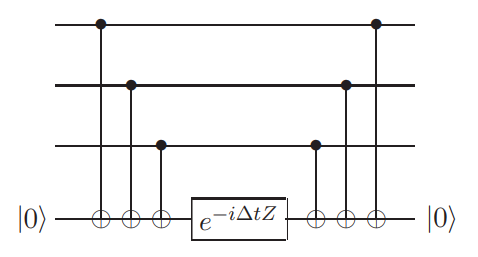
\includegraphics[width=0.5\linewidth]{Images/Ham-sim-circ.png}
%     \caption{Quantum circuit for simulation the Hamiltonian $H=Z_1 \otimes Z_2 \otimes Z_3$ for time $\Delta t$}
%     \label{fig:ham_sim_circ}
% \end{figure}
% Furthermore, extending the same procedure allows us to simulate more complicated extended Hamiltonians. Specifically, we can efficiently simulate any Hamiltonian of the form
% \[
% H=\otimes_{k=1}^n \sigma_{c(k)}^k
% \]
% where $\sigma_{c(k)}^k$ is a Pauli matrix (or the identity) acting on the kth qubit, with $c(k)\in\{0,1,2,3\}$ specifying one of $\{I,X,Y,Z\}$. The qubits upon which the identity operation is performed can be disregarded, and $X$, or $Y$ terms can be transformed by single qubit gates to $Z$ operations. This leaves us with a Hamiltonian of the form, which is simulated as described above.

% The circuit shown in figure \ref{fig:ham_sim_circ} simulates $e^{-\iota H\Delta t}=e^{-\iota \Delta t (Z_1\otimes Z_2\otimes Z_3)}$. All this can be done because we use the property that $e^{\iota Ax}=\cos x I-\iota \sin x A $ when $A^2=I$. Note that the $(\sigma_1\otimes \sigma_2\otimes \ldots \otimes \sigma_n)^2=I$ where $\sigma_i$ are any one of the Pauli matrices acting on their respective qubits. This is because $(\otimes_{i=1}^n \sigma_i)(\otimes_{i=1}^n \sigma_i)=(\otimes_{i=1}^n \sigma_i^2) = I$. This can be shown as follows:
% \begin{align*}
%     e^{-\iota \Delta tZ_1 \otimes Z_2 \otimes Z_3}\ket{abc} &=  (\cos \Delta t I - \iota \sin \Delta t (Z_1\otimes Z_2\otimes Z_3))\ket{abc} \\
%     &=(\cos \Delta t I\ket{abc} - \iota\sin \Delta t (Z_1\otimes Z_2\otimes Z_3)\ket{abc}\\
%     &=(\cos \Delta t \ket{abc}- \iota\sin \Delta t (-1)^{a+b+c} \ket{abc}\\
%     &=\cos \Delta t \ket{abc} - (-1)^{a+b+c}\iota \sin \Delta t \ket{abc}\\
%     &=(\cos \Delta t - (-1)^{a+b+c}\iota \sin \Delta t)\ket{abc}\\
%     &=\begin{cases} e^{-\iota \Delta t}\ket{abc} &\text{if the parity is even for $n$ qubits}\\
% e^{\iota \Delta t} \ket{abc}&\text{if the parity is odd for $n$ qubits} \end{cases}
% \end{align*}
% which is what is implemented by the circuit shown in figure \ref{fig:ham_sim_circ}, where the result will be $e^{-\iota \Delta t}$ if the parity is even for $n$ qubits and $e^{\iota \Delta t}$ if the parity if odd for $n$ qubits.
% \begin{example}
%     Construct a quantum circuit to simulate the Hamiltonian
%     \[
%     H=X_1\otimes Y_2\otimes Z_3
%     \]
%     performing the unitary transformation $e^{-\iota \Delta tH}$ for any $\Delta t$.

%     Recall the matrix identities,
%     \[
%     X = HZH; \quad Y=R_X\left(-\frac{\pi}{2}\right)ZR_X\left(\frac{\pi}{2}\right)
%     \]
%     Thus, using this single qubit gates we can write the Hamiltonian as follows:
%     \[
%     H = (H \otimes R_X\left(-\frac{\pi}{2}\right) \otimes I)(Z_1 \otimes Z_2 \otimes Z_3)(H\otimes R_X\left(\frac{\pi}{2}\right)\otimes I)
%     \]
%     Now, we are required to simulate $U=e^{-\iota (X_1\otimes Y_2 \otimes Z_3)\Delta t}$. We can thus, simplify this as follows:
%     \begin{align*}
%         U&=e^{-\iota (X_1 \otimes Y_2 \otimes Z_3)\Delta t}\\
%         &=\cos \Delta t I_1 \otimes I_2 \otimes I_3 -\iota \sin \Delta t X_1 \otimes Y_2 \otimes Z_3\\
%         &=(H_1\otimes R_X\left(-\frac{\pi}{2}\right) \otimes I)(\cos \Delta t I_1 \otimes I_2 \otimes I_3-\iota \sin \Delta t Z_1 \otimes Z_2 \otimes Z_3)(H_1 \otimes R_X\left(\frac{\pi}{2}\right) \otimes I_3)\\
%         &=(H_1\otimes R_X\left(-\frac{\pi}{2}\right) \otimes I)e^{-\iota Z_1\otimes Z_2 \otimes Z_3 \Delta t}(H_1 \otimes R_X\left(\frac{\pi}{2}\right) \otimes I_3)
%     \end{align*}
% \end{example}
% Using this procedure allows us to simulate a wide class of Hamiltonians containing terms which are not local. In particular, it is possible to simulate a wide class of hamiltonians containing terms which are not local. In particular, it is possible to simulate a Hamiltonian of the form $H=\sum_{k=1}^L H_k$ where the only restriction is that the individual $H_k$ have a tensor product structure, and that $L$ is a polynomial in the total number of particles $n$. More generally, all that is required is that there be an efficient circuit to simulate each $H_k$ separately. As an example, the Hamiltonian $H=\sum_{k=1}^n X_k + Z^{\otimes n}$ can be easily simulated using the above techniques. Such Hamiltonians typically do not arise in Nature. However, they provide a new and possibly valuable vista on the world of quantum algorithms.

% \section{Commutator type error bound}
% In this section we try to refine the error bounds in the equation by evaluating the preconstant explicitly. For simplicity we focus only on the first order Trotter formula. The trotter propagator $\tilde{U}(t)=e^{-\iota tH_1}e^{-\iota tH_2}$ satisfies the equation
% \begin{align*}
% \iota \partial_t\tilde{U}(t)&=e^{-\iota tH_1}e^{-\iota tH_2}+e^{-\iota tH_1}H_2e^{-\iota tH_2}\\
% &=(H_1+H_2)e^{-\iota tH_1}e^{-\iota tH_2}+e^{-\iota t H_1}H_2e^{-\iota tH_2}-H_2e^{-\iota t H_1}e^{-\iota t H_2}\\
% &=H\tilde{U}(t)+[e^{-\iota t H_1},H_2]e^{-\iota t H_2}
% \end{align*}
% with initial condition $\tilde{U}(0)=I$. By Duhamel's principle, and let $U(t)=e^{-\iota tH}$, we have
% \[
% \tilde{U}(t)=U(t)-\iota \int_0^t e^{-\iota H(t-s)}[e^{-\iota sH_1},H_2]e^{-\iota sH_2} ds
% \]
% So we have
% \[
% \|\tilde{U}(t)-U(t)\|\leq \int_0^t \|e^{-\iota s H_1},H_2\|ds
% \]
% Now consider $G(t)=[e^{-\iota t H_1},H_2]e^{\iota t H_1}=e^{-\iota tH_1}H_2e^{\iota t H_1}-H_2$, which satisfies $G(0)=0$ and
% \[
% \iota \partial_tG(t)=e^{-\iota t H_1} [H_1,H_2]e^{+\iota t H_1}
% \]
% Hence,
% \[
% \|[e^{-\iota t H_1},H_2]\|=\|G(t)\|\leq t\|[H_1,H_2]\|
% \]
% Plugging this back to Equation we have
% \[
% \|\tilde{U}9T)-U(t)\|\leq \int_0^t s\|[H_1,H_2]\|ds \leq \frac{t^2}{2}\|[H_1,H_2]\|\leq t^2\nu^2
% \]
% In the last equality, we have used the relation $\|[H_1,H_2]\| \leq 2\nu^2$ with $\nu = \max\{\|H_1\|,\|H_2\|\}$. Therefore equation can be replaced by a sharper inequality
% \[
% \|e^{-\iota \Delta tH}-e^{-\iota \Delta t H_1}e^{-\Delta tH_2}\|\leq \frac{\Delta t^2}{2} \|[H_1,H_2]\|\leq (\Delta t)^2\nu^2
% \]
% Here the first inequality is called the commutator norm error estimate, and the second inequality the operator norm error estimate.

% For the transverse field Ising model with nearest neighbor interaction, we have $\|H_1\|,\|H_2\|=\mathcal{O}(n)$, and hence $\nu^2=\mathcal{O}(n^2)$. On the other hand, since $[Z_iZ_j,X_k]\neq 0$ only if $k=i$ or $k=j$, the commutator bound satisfies $\|H_1,H_2]\|=\mathcal{O}(n)$. therefore to reach precision $\epsilon$, the scaling of the total number of time steps $L$ with respect to the system size is $\mathcal{O}(n^2/\epsilon$ according to the estimate based on the operator norm, but is only $\mathcal{O}(n/\epsilon)$ according to that based on the commutator norm.

% For the particle in a potential, for simplicity consider $d=1$ and the domain $\Omega=[0,1]$ is discretized using a uniform grid of size $N$. For smooth and bounded potential, we have $\|H_1\|=\mathcal{O}(N^2)$, and $\|V\|=\mathcal{O}(1)$. therefore the operator norm bound gives $\nu^2=\mathcal{O}(N^4)$. This is too pessimistic. Reexamining the second inequality of the equation shows that in this case, the error bound should be $\mathcal{O}((\Delta t)^2\nu)$ instead of $(\Delta t)^2 \nu^2$. So according to the operator norm error estimate, w have $L=\mathcal{O}(N^2/\epsilon)$. On the other hand, in the continuous space, for any smooth function $\psi(r)$, we have
% \[
% [H_1,H_2]\psi=\left[-\frac{d^2}{dr^2},V\right]\psi=-V''\psi-V'\psi'
% \]
% So
% \[
% \|H_1,H_2]\psi\|\leq \\V''\|+\|V'\|\|\psi'\|=\mathcal{O}(N)
% \]
% here we have used that $\|V'\|=\|V''\|=\mathcal{O}(1)$, and $\|\psi'\|=\mathcal{O}(N)$ in the worst case scenario. therefore $\|[H_1,H_2]\|=\mathcal{O}(N)$, and we obtain a significantly improved estimate $L=\mathcal{O}(N/\epsilon)$ according to the commutator norm.

% The commutator scaling of the trotter error is an important feature of the method. there are papers for analysis of the second order Trotter method, and for the analysis of the commutator scaling of high order trotter methods.

% \begin{remark}
%     (vector norm bound). The Hamiltonian simulation problem of interest in practice often concerns the solution with particular types of initial conditions, instead of arbitrary initial conditions. Therefore the operator norm bound in the equation can still be too loose. Taking the initial condition into account, we readily obtain
%     \[
%     \|e^{-\iota |delta tH}\psi(0)-e^{\-iota \Delta tH_1}e^{-\iota \delta tH_2}\psi(0)\|\leq \frac{\Delta t^2}{2}\max_{0\leq s \leq \Delta t} \|[H_1,H_2]\psi(s)\|
%     \]
%     For the example of the particle in a potential, we have
%     \[
%     \max_{0\leq s\leq \Delta t} \|[H_1,H_2]\psi(s)\|\leq \|V''\|+\|V'\| \max_{0\leq s \leq \Delta t} \|\psi'(s)\|
%     \]
%     Therefore, if we are given the a priori knowledge that $\max_{0\leq s \leq t} \|\psi'(s)\|=\mathcal{O}(1)$, we may even have $L=\mathcal{O}(\epsilon^{-1})$, i.e., the number of time steps is independent of $N$.
% \end{remark}

% \begin{example}
%     Consider the Hamiltonian simulation problem for $H=H_1+H_2+H_3$. Show that the first order Trotter formula
%     \[
%     \tilde{U}(t)=e^{-\iota t H_1}e^{-\iota t H_2}e^{-\iota t H_3}
%     \]
%     has a commutator type error bound.
% \end{example}
% \begin{example}
%     Consider the time-independent Hamiltonian simulation problem for the following controlled Hamiltonian
%     \[
%     H(t)=a(t)H_1+b(t)H_2
%     \]
%     where $a(t)$ and $b(t)$ are smooth functions bounded together will all derivatives. We focus on the following trotter type splitting, defined as
%     \[
%     \tilde{U}(t):=\tilde{U}(t_n,t_{n-1})\ldots \tilde{U}(t-1,t_0), \quad \tilde{U}(t_{j+1},t_j)=e^{-\iota \Delta ta(t_j)H_1}e^{-\iota \Delta tb(t_j)H_2}
%     \]
%     where the intervals $[t)j,t_{j+1}]$ are equidistant and of length $\Delta t$ on the interval $[0,t]$ with $t_n=t$. Show that this method has first-order accuracy, but does not exhibit a commutator type error bound in general.
% \end{example}

% \chapter{The Adiabatic Algorithm}
% \section{The Local Hamiltonians}
% We saw that the following problem is NP-hard:\\
% Given as input an $n$-qubit Hamiltonian of the form $H=H_1 +\ldots+H_m$, with each $H_i$, acting on at most $3$ of the $n$ qubits, estimate $H's$ ground state energy. We call this problem the Local Hamiltonians Problem. This is a quantum generalization of the 3SAT problem which arises very naturally in condensed matter physics.

% How do you give someone a Hamiltonian like that? Proviging the full $2^n \times 2^n$ Hermitian matrix would be wasteful. Instead you can simply list the local terms $\{H_0,\ldots,H_{m-1}\}$ (to some suitable precision), togehter with the qubits to which they're applied.

% Is this problem NP-complete? Since we know it's NP-hard, what we're asking here is whether it's also in NP. In other words, when we claim that the ground-state energy of some Hamiltonian is at most (say) 5, can we prove it by giving a short witness? It turns out that we can, but as far as anyone knows only by giving a quantum witness! A quantum witness that works is simply the $n$-qubti ground state itself. Thus, the Local Hamiltonians problem is not known to be in NP; it's only known to be in the quantum analogue of NP, which is called QMA (Quantum Merlin-Arthur). An important theorem from around 1999 says that Local Hamiltonain is actually complete for QMA, just like 3SAT is complete for NP. For the specific Hamiltonian $H$ we constructed in the last chapter - the one that encoded 3 SAT - there would be a short classical witness. Because $H$ wa a diagonal ma







% \chapter{The HHL Algorithm}
% \section{Introduction}
% The Harrow-Hassidim-Lloyd (HHL) \cite{harrow2009quantum} 
% algorithm for solving large systems of linear equations.
% Linear system of equations arise in almost any real-life applications from Physics, Maths and Engineering
% to Finanical and Biological Sciences. Typical examples of real-life problems involving solving system of linear equations computationally include, 
% solutions of Partial Differential Equations, the calibration of financial models, fluid simulation 
% of numerical field calculation, optimization, machine learning etc. 
% Most real-life problems generally boils down to a set of Linear Equations. We even approximate 
% non-linear terms in non-linear equations, to linear terms in order to approximate the non-linear equations to linear equations in few cases.

% \section{The Linear-System Problem (LSP)}
% The classical linear-system problem is defined as follows:
% \begin{definition}
% Given a matrix $A\in \mathbb{C}^{N \times N}$ and a vector $\vec{b} \in \mathbb{C}^N$, find $\vec{x} \in \mathbb{C}^N$
% satisfying $A\vec{x}=\vec{b}$.
% \end{definition}

% In most of the applications it sufficies to find 
% $\vec{x}$ such that $\|\vec{x}-\vec{x}_0\|<\epsilon$ for some $\epsilon>0$, 
% where $\vec{x}_0$ is the exact solution.
% Assuming that $A$ is invertible (or $rank(A)=N$ i.e. full rank)
% for simplicity, the solution to the above problem is given by $\vec{x}=A^{-1}\vec{b}$.
% In case, $A$ is not invertible, we can use the Moore-Penrose Pseudo-Inverse of $A$ to get the solution which is 
% $\vec{x}=(A^{\dagger}A)^{-1}A^{\dagger}\vec{b}$, where $(A^{\dagger}A)^{-1}A^{\dagger}$ is called the Moore-Penrose Psuedo-Inverse of A.

% A system of linear equations is called \textbf{$s$-sparse if $A$ has at most $s$ non-zero entries per row or column}. 
% Solving an $s$-sparse system of size $N$ with a classical computer requires $O(Ns\kappa \log (1/\epsilon))$ time complexity
% using the conjugate gradient method \cite{shewchuk1994introduction}. Here, $\kappa$ is the condition number of the system and 
% $\epsilon$ is the accuracy of the approximation. Overall, the solution on a classical computer is simply $x=A^{-1}b$. Note that here the solution x is not necessarily a normalized vector, and hence cannot be stored as a quantum state. Thus, for solving the problem on a Quantum Computer we define the corresponding QLSP which is the quantum equivalent of the classical LSP.

% The Quantum Linear-System Problem (QLSP) is defined as follows:
% \begin{definition}
% Given a matrix $A\in \mathbb{C}^{N \times N}$ and $\ket{b} \in \mathbb{C}^N$, find $\ket{\tilde{x}} \in \mathbb{C}^N$
% such that $\|\ket{x}-\ket{\tilde{x}}\|\leq \epsilon$ for some $\epsilon>0$ where $\ket{x}$ is the exact solution
% satisfying $A\ket{x}=\ket{b}$.
% \end{definition}

% For simplicity, we assume $\ket{b}$ is normalized and can be efficiently implemented using a transformation $U_b$ (has a efficient quantum circuit) as a $n_b$ qubit quantum state. Here, the goal is to produce an n-qubit state whose amplitude-vector (up to normalization and up to $\epsilon$ error) 
% is a solution to the linear system. Thus,
% \[
% \|\ket{x}-\tilde{\ket{x}}\|\leq \epsilon,\quad \ket{x}=\frac{A^{-1}\ket{b}}{\|A^{-1}\ket{b}\|}
% \]
% We are required to find the normalization constant $\|A^{-1}\ket{b}\|$ separately. Note that here $\tilde{\ket{x}}$ will be in a superposition state, thus in order to estimate the amplitude/coefficients it is required to do a lot of experiments. 

% The HHL algorithm requires $A$ to be Hermitian. We can create any given general matrix $A$ to a Hermitian Matrix using the following method called \textbf{Dilation method}.

% \textbf{Without the loss of generality we can assume that A (through this we can convert the general matrix A given in classical LSP to a Hermitian matrix for QLSP) is Hermitian since any matrix A can be made Hermitian using the following method.
% We define $A'$ as:}
% \[
% A'=\begin{bmatrix} 0 & A \\ A^{\dagger} & 0 \end{bmatrix}=\ket{1}\bra{0}\otimes A+ \ket{0}\bra{1}\otimes A^{\dagger}
% \]
% \textbf{and thus, the problem now can be defined as:}
% \[
% \begin{bmatrix} 0 & A \\ A^{\dagger} & 0 \end{bmatrix} \begin{bmatrix} \ket{0} \\ \ket{x} \end{bmatrix} = \begin{bmatrix} \ket{b} \\ \ket{0} \end{bmatrix}
% \]
% \textbf{thus preserving the original problem $A\ket{x}=\ket{b}$. Thus, $A'\ket{x}'=\ket{b}'$ where 
% $\ket{x}'=\begin{bmatrix} \ket{0}\\ \ket{x} \end{bmatrix}, \ket{b}'=\begin{bmatrix}\ket{b}\\ \ket{0} \end{bmatrix}$
% and $A'$ is Hermitian ($A'^{\dagger}=A'$). Thus for a given problem in classical LSP as $A\ket{x}=\ket{b}$, we can convert
% it to a QLSP problem as $A'\ket{x}'=\ket{b}'$ where $A'$ is Hermitian using the above method. Thus, without the loss of generality for the application of 
% HHL algorithm we can assume that the matrix A is Hermitian.}

% The HHL algorithm estimates a function of the solution with time complexity of $O(log(N)s^2\kappa^2/\epsilon)$.
% The \textbf{assumptions/restrictions} on the Linear system in order to make the HHL algorithm work are:
% \begin{enumerate}
% \item \textbf{Assume that b is normalized: (hence can be stored in a quantum state) }We have a unitary matrix $U_b$ which can prepare $\ket{b}$ as an n-qubit quantum state $\ket{b}=\frac{1}{\|b\|}\sum_ib_i\ket{i}$
%     using a circuit of B 2-qubit gates. We also assume for simplicity that $\|b\|=1$.
%     Thus, it is possible that using some work registers $\ket{0}_{n_b}$ to transform it to $\ket{b}$ using the transformation as shown:
%     \[
%         \ket{0^{n_b}} \xrightarrow{U_b} \ket{b}_{n_b}
%     \]
% \item The matrix A is s-sparse and we have sparse access to it. Such sparsity is not essential to the algorithm, and could be replaced by other properties that enable an efficient
%     block-encoding of A.
% \item The matrix A is well-conditioned: (A is invertible, thus $\kappa$ is some finite value) The ratio between its largest and smallest singular value
%     is at most some $\kappa$. For simplicity, assume the smallest singular value is $\geq 1/\kappa$ while the largest is $\leq1$. In other words, all eigenvalues of A lie in the 
%     interval $[-1,-1/\kappa] \cup [1/\kappa,1]$. The smaller the condition number $\kappa$ is, the better it will be for the algorithm. Let's assume our algorithm knows $\kappa$, or at least knows a reasonable 
%     upper bound on $\kappa$.
% \end{enumerate}

% \section{The HHL Algorithm}
% \subsection{Some Mathematical Preliminaries}
% To encode the problem on a quantum computer we need to rescale the system, by assuming $b$ and $x$ to be normalized and map them to the respective quantum states $\ket{b}$ and $\ket{x}$. The ith component of $\ket{b}$ corresponds to the amplitude of the ith basis state of the quantum state $\ket{b}$. Thus, we now focus on the rescaled problem
% \[
% A\ket{x}=\ket{b}
% \]
% Since A is Hermitian ($A^{\dagger}=A$) thus, a Normal Matrix ($AA^{\dagger}=A^{\dagger}A$), hence Unitarily diagonalizable as:
% \[
%     A=U\Lambda U^{\dagger}
% \]
% where $U$ is a unitary matrix made up of the eigenvectors of A and $\Lambda$ is a diagonal matrix with the eigenvalues of A on the diagonal.
% It's spectral decomposition can be written in outer product form as:
% \[
%     A=\sum_{j=0}^{N-1}\lambda_j\ket{\lambda_j}\bra{\lambda_j}, \quad \lambda_j\in \mathbb{R}
% \]
% where $\ket{\lambda_j}$ are the eigenvectors of A and $\lambda_j$ are the corresponding eigenvalues.
% Then,
% \begin{align*}
%     A^{-1}&=(U\Lambda U^{\dagger})^{-1}\\
%     &=U\Lambda^{-1}U^{\dagger}
% \end{align*}
% Thus spectral decomposition of $A^{-1}$ is:
% \[
%     A^{-1}=\sum_{j=0}^{N-1}\lambda_j^{-1}\ket{\lambda_j}\bra{\lambda_j}
% \]
% Now, since A is unitarily diagonalizable thus, it forms a complete basis set of orthonormal eigenvectors $\{\ket{\lambda_j}\}$ 
% which span the $\mathbb{C}^N$ space. Thus, any vector $\ket{v}$ can be written as a linear combination of the eigenvectors of A. Thus,
% we write the right hand side of the system $\ket{b}$ as:
% \[
%     \ket{b}=\sum_{j=0}^{N-1}b_j\ket{\lambda_j}, \quad b_j\in \mathbb{C}
% \]
% The goal of the HHL algorithm is to exit with the readout register in the state
% \begin{align*}
%     \ket{x}=A^{-1}\ket{b}&=\left(\sum_{j=0}^{N-1}\lambda_j^{-1}\ket{\lambda_j}\bra{\lambda_j}\right)\left(\sum_{k=0}^{N-1}b_k\ket{\lambda_k}\right)\\
%     &=\left(\sum_{j=0}^{N-1}\sum_{k=0}^{N-1}b_k\lambda_j^{-1}\ket{\lambda_j}\braket{\lambda_j|\lambda_k}\right)\\
% \end{align*}
% Now $\braket{\lambda_j|\lambda_k}=\delta_{jk}$ (because A is a Hermitian matrix, thus Unitarily diagonalizable and hence has orthonormal eigenvectors), thus the above expression simplifies to:
% \[
%     \ket{x}=\sum_{j=0}^{N-1}b_j\lambda_j^{-1}\ket{\lambda_j}
% \]
% which is the required solution to the linear system $A\ket{x}=\ket{b}$.

% \subsection{Algorithm}
% Consider the following circuit as shown in the figure \ref{fig:hhl_circuit}. The first qubit show is initialised to $\ket{0}$ which is also called the signal qubit. The algorithm uses three quantum register, all set to $\ket{0}$ at the beginning of the algorithm. One register, which we will denote with the subindex $n_l$, is used to store a binary representation of the eigen values of $A$. A second register, denoted by $n_b$, contains the vector solution. Note that $N=2^{n_b}$. There is an extra register, which we will denote with $n_a$ for auxillary qubits, used for intermediate steps in the computation. We can ignore any auxillary in the following description as they are $\ket{0}$ at the beginning of each computation, and are restored back to $\ket{0}$ at the end of each individual operation.
% \begin{figure}[ht]
%     \centering
%     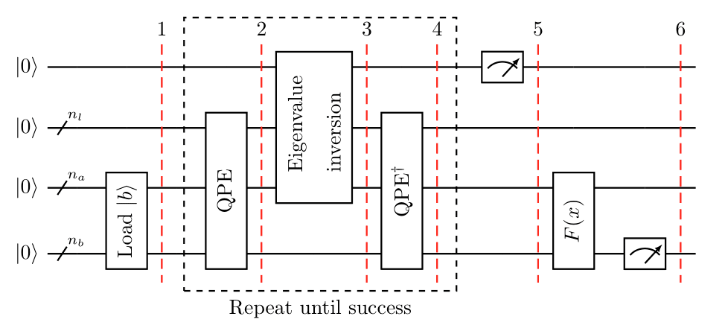
\includegraphics[width=0.9\textwidth]{Images/hhl_circuit.png}
%     \caption{HHL Circuit}
%     \label{fig:hhl_circuit}
% \end{figure}

% \textbf{Analysis:}\\
% Let us now analyze the working of the above circuit (note that we ignore the ancilla registers throughout the analysis):
% \begin{enumerate}
%     \item Load the data $\ket{b} \in \mathbb{C}$. That is, perform the transformation
%     \[
%         \ket{0}\ket{0}_{n_l}\ket{0}_{n_b} \xrightarrow{I\otimes I\otimes U_b} \ket{0}\ket{0}_{n_l}\ket{b}_{n_b}
%     \]
%     \item Now we are required to apply QPE. Ignoring the Ancilla bits, recall that in QPE given a Unitary matrix $U$ and one of its eigen vector $\ket{\psi}$,
%     we can find the eigenvalue $e^{\iota 2\pi \theta}$ corresponding to $\ket{\psi}$ (or specifically approximate $\theta$ i.e. $\tilde{\theta}$ upto d bits of accuracy) by applying the QPE algorithm,
%     where $\theta \approx \tilde{\theta} \in [0,1)$. Thus, we have the following transformation:
%     \[
%         \ket{0^d}\ket{\psi}\xrightarrow{U_{QPE}} \ket{\tilde{\theta}}\ket{\psi}
%     \]
%     where $\ket{\tilde{\theta}}$ is a d-bit (in binary) basis state in the computational basis corresponding to the closest binary representation of the actual phase $\theta \in [0,1)$ that corresponds to the eigen vector $\ket{\psi}$.
%     Thus, first we require a Unitary matrix, here we are required to form a Unitary matrix using A which is a Hermitian matrix.
%     Let us define $U=e^{\iota 2\pi At}$ where t is some scalar prescaling factor and U is a Unitary matrix (exponential of a Hermitian matrix results in a unitary matrix). Now,
%     \[
%         e^{\iota 2\pi At}=I+\iota 2\pi At-\frac{1}{2}(2\pi)^2A^2t^2-\frac{\iota}{6}(2\pi)^3 A^3t^3+\ldots
%     \]
%     We know that $A=Q\Lambda Q^{\dagger}$, since A is unitarily diagonalizable for some orthonormal matrix Q, upon substituting and simplifying, we get, $e^{\iota 2\pi At}=Qe^{\iota 2\pi \Lambda t}Q^{\dagger}$.
%     Upon writing this in outer product/spectral decomposition form we get,
%     \[
%         U=e^{\iota 2\pi At}=\sum_{j=0}^{N-1}e^{\iota 2\pi \lambda_j t}\ket{\lambda_j}\bra{\lambda_j}
%     \]
%     Thus, U and A share the same eigen vectors but the eigen values of $At$ are $2\pi \lambda_jt$ and the eigen values of U are $e^{\iota 2\pi \lambda_j t}$, thus we can apply QPE to find the eigen values of A. Also recall that since A is Hermitian matrix, thus, the eigen values of A i.e. $\lambda_j \in \mathbb{R} \forall j$. Using QPE, we can find approximate values of the phases and thus, we can write,
%     $e^{\iota 2\pi \tilde{\theta_j}}\approx e^{\iota 2\pi \lambda_j t} \implies \tilde{\theta_j}\approx \lambda_j t$ (recall that $\tilde{\theta_j}\in [0,1)$ which is an approximation to the exact phase $\theta_j$),
%     Upon rearranging the terms we get,
%     \[
%         \lambda_j \approx \frac{\tilde{\theta_j}}{t}
%     \]
%     for each $j \in \{0,\ldots,N-1\}$. Recall, that here t is not known to us, thus we need to estimate it.
%     We use this prescaling factor in order to map the eigen values of A to the range $[0,1)$. There are various methods to estimate t so that the Eigenvalues of A are in the range $[0,1)$. Without getting involved on how to find t, we assume that we know the value of t so that the eigen values of A are in $[0,1)$. Let this new eigen values be $\tilde{\theta_j} \approx \lambda_j'=\lambda_j t$ such that $0 \leq lambda_0'\leq \lambda_1' \leq \lambda_2' \leq \ldots \leq\lambda_{N-1}' < 1$. Thus,
%     \[
%     \tilde{\theta_j} \approx \lambda_j' \quad \forall \quad j \in \{0,\ldots,N-1\}
%     \]
%     Thus, the phases are approximations to the shifted eigenvalues to be in range $[0,1)$.
%     Here, the QPE problem is as shown in the figure \ref{fig:qpe}.
%     \begin{figure}[ht]
%         \centering
%         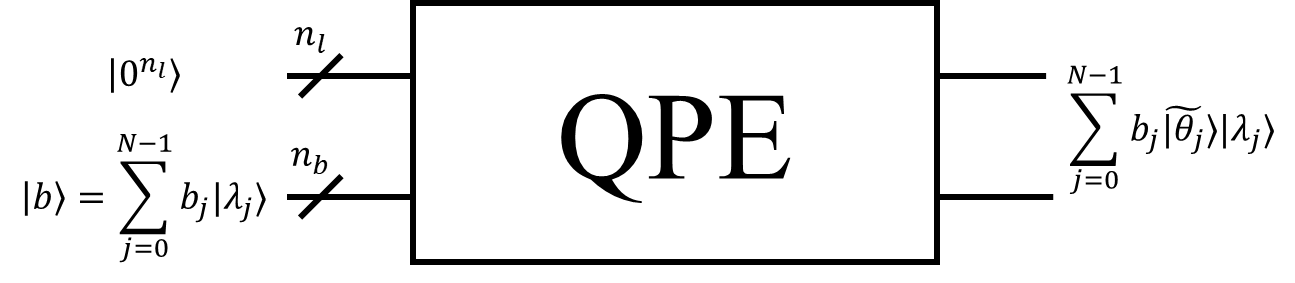
\includegraphics[width=0.7\textwidth]{Images/qpe.png}
%         \caption{QPE}
%         \label{fig:qpe}
%     \end{figure}
%     Note that the input to the QPE is not an eigen state but as shown in the figure \ref{fig:qpe}, 
%     it is a superposition of the eigen states of A, i.e. $\ket{b}=\sum_{j=0}^{N-1}b_j\ket{\lambda_j}$.
%     Thus, the resulting output will be a superposition of $\tilde{\theta_j}$ i.e. $\sum_{j=0}^{n-1}b_j\ket{\tilde{\theta_j}}\ket{\lambda_j}$.
%     Here, $\ket{\tilde{\theta_j}}$ is one of the basis states in the computational basis corresponding to the 
%     closest binary representation of the actual phase $\theta_j=\lambda_j'=\lambda_jt$ that corresponds to the eigen vector $\ket{\lambda_j}$.
%     In other words, say the actual phase corresponding to a eigen state $\ket{\lambda_j}$ is $\theta_j \in [0,1)$
%     Thus, $\theta_j\approx 0.\theta_{j_{n_l-1}}\theta_{j_{n_l-2}}\ldots\theta_{j_0}=\tilde{\theta_j}$ is the $n_l$ bit binary approximation of $\theta_j$.
%     Thus, the output of the QPE will be a superposition of the $n_l$ bit binary approximations of the actual phases $\theta_j$.
%     At the end of this transformation we get,
%     \[
%         \ket{0}\ket{0}_{n_l}\ket{0}_{n_b} \xrightarrow{I\otimes QPE}  \ket{0}\sum_{j=0}^{N-1}b_j\ket{\tilde{\theta_j}}\ket{\lambda_j}
%     \]
%     where $\tilde{\theta_j}$ are binary approximations of the eigen values of A in the range $[0,1)$ corresponding to the eigen vector $\ket{\lambda_j}$.
%     \item \textbf{Implementation of the controlled rotations: }Now we are suppose to inverse the eigen values in order to achieve the aim of getting
%     \[
%     \sum_{j=0}^{N-1} \lambda_j^{-1} b_j\ket{\tilde{\theta_j}}\ket{\lambda_j}
%     \]
%     from
%     \[
%     \ket{0}\sum_{j=0}^{N-1}b_j\ket{\tilde{\theta_j}}\ket{\lambda_j}
%     \]
%     In order to do this we are required to implement controlled rotations.
%     Let us take a slight diversion from the algorithm to learn about the implementation of controlled rotation in order to implement it efficiently for the algorithm. Consider the following proposition.
%     \begin{proposition}
%         (Controlled rotation given rotation angles). Let $0\leq \theta <1$ has exact d-bit fixed point representation $\theta=0.\theta_{d-1}\ldots\theta_0$ be its d-bit fixed point representation. Then there is a (d+1)qubit unitary $U_{\theta}$ such that
%         \[
%         U_{\theta}:\ket{0}\ket{\theta}\rightarrow (\cos (\pi \theta) \ket{0} + \sin (\pi\theta) \ket{1})\ket{0}
%         \]
%     \end{proposition}
%     \begin{proof}
%         Recall that $R_Y$ gate is as follows:
%         \[
%         R_{\theta}^Y=R_Y(\theta)=e^{-\iota \frac{\theta}{2}\sigma_Y}=\begin{bmatrix} \cos (\theta/2) & -\sin (\theta/2) \\ \sin (\theta/2) & \cos (\theta/2) \end{bmatrix}
%         \]
%         Now putting $\theta=2\tau$ we get
%         \[
%         R_Y(2\tau) =e^{\iota \tau \sigma_Y}=\begin{bmatrix} \cos (\tau) & -\sin(\tau) \\ \sin(\tau) & \cos (\tau) \end{bmatrix}
%         \]
%         Here $R_Y(.)$ performs a single-qubit rotation around the y-axis. For any $j \in \{0,\ldots,2^d-1\}$ with its binary representation $j=j_{d-1}\ldots j_0$, we have
%         \[\frac{j}{2^d}=(0.j_{d-1}\ldots j_0)\]
%         So we choose $\tau=\pi(0.j_{d-1}\ldots j_0)$, which can be further simplified putting $j_k=\theta_k \forall k \in\{d-1,\ldots,0\}$. Thus, we define
%         \begin{align*}
%         U_{\theta}&=\sum_{j=0}^{N-1} e^{-\iota \pi(0.j_{d-1}\ldots j_0)\sigma_Y} \otimes \ket{j}\bra{j}\\
%         &=\sum_{\theta_{d-1},\dots,\theta_0}e^{-\iota \pi(0.\theta_{d-1}\ldots \theta_0)\sigma_Y} \otimes \ket{\theta_{d-1}\ldots\theta_0}\bra{\theta_{d-1}\ldots\theta_0}
%         \end{align*}
%         \begin{align*}
%         U_{\theta}&=\sum_{\theta_{d-1},\ldots,\theta_0} e^{-\iota \pi\frac{\theta_{d-1}}{2}\sigma_Y}e^{-\iota \pi\frac{\theta_{d-2}}{4}\sigma_Y}\ldots e^{-\iota\pi \frac{\theta_0}{2^{d}}\sigma_Y} \otimes \ket{\theta_{d-1}\ldots\theta_0}\bra{\theta_{d-1}\ldots\theta_0}\\
%         &=\sum_{\theta_{d-1},\ldots,\theta_0} R_Y(\pi\theta_{d-1}) R_Y(\pi\frac{\theta_{d-2}}{2}) \ldots R_Y(\pi\frac{\theta_0}{2^{d-1}}) \otimes \ket{\theta_{d-1}\ldots\theta_0}\bra{\theta_{d-1}\ldots\theta_0}\\
%         &=\sum_{\theta_{d-1},\ldots,\theta_0} R_Y(\pi\theta_{d-1})R_Y(\frac{\pi}{2}\theta_{d-2})\ldots R_Y(\frac{\pi}{2^{d-1}}\theta_0) \otimes \ket{\theta_{d-1}\ldots\theta_0}\bra{\theta_{d-1}\ldots\theta_0}
%         \end{align*}
%         Thus, applying $U_{\theta}$ to $\ket{0}\ket{\theta}$ gives the desired result since corresponding to a particular value of $\theta$ only one of the terms from the summation with which its inner product results in 1 will survive (since all the basis states are orthonormal).
%         The resulting quantum circuit for the controlled rotation is as shown in the figure \ref{fig:controlledrotation}.
%         \begin{figure}
%             \centering
%             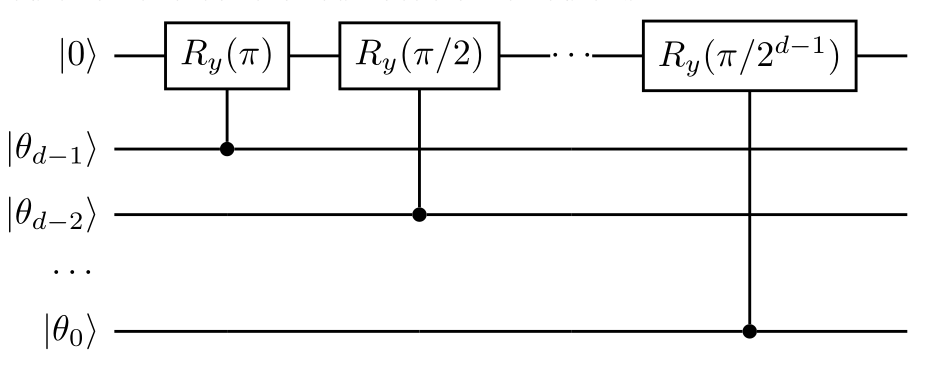
\includegraphics[width=\linewidth]{Images/Controlledrotation.png}
%             \caption{Controlled Rotation}
%             \label{fig:controlledrotation}
%         \end{figure}
%     \end{proof}
%     Thus, as shown in the circuit in figure \ref{fig:controlledrotation} based upon the input binary state of $\theta_{d-1}\ldots\theta_0$ the corresponding $R_Y$ gates will be acted on the signal bit (which was initialised to $\ket{0}$) where each $\theta_k$ will act as the control bit for the corresponding $R_Y(\pi/2^{d-k-1})$.

%     In other words, the controlled rotation implementation will perform a transformation as:
%     \[
%     U_{\phi}\ket{0}\ket{\phi} \rightarrow (\cos (\pi\phi)\ket{0} + \sin (\pi\phi)\ket{1})\ket{\phi}
%     \]
%     where $\phi \in [0,1)$.
%     This is a sequence of single-qubit rotations on the signal qubit, each controlled by a single qubit.

%     Back to the problem, we are required to inverse the eigen values which can be done using implementation of controlled rotation operation. Say we define
%     \[
%     \phi_j=\frac{1}{\pi}\sin^{-1}(C/\tilde{\theta_j})
%     \]
%     where $C>0$ be a lower bound to $\lambda_0'$, so that $0<C/\tilde{\theta_j}<1$ for all $j$. Recall that $\tilde{\theta_j}\approx \lambda_j'$ and $\tilde{\theta_j} \in [0,1)$. Writing all of this in d' bit binary representation we get,
%     \[
%     \tilde{\phi_j}=\frac{1}{\pi}\sin^{-1}(C/\tilde{\theta_j'})\approx \phi_j= \frac{1}{\pi}\sin^{-1}(C/\tilde{\theta_j})
%     \]
%     For simplicity, we assume that d' is large enough so that the error of the fixed point representation is negligible in this step. The mapping
%     \[
%     U_{angle}\ket{0^{d'-d}}\ket{\tilde{\theta_j}}=\ket{\tilde{\phi_j}}
%     \]
%     can be implemented using \textit{classical arithmetics circuits}, which may require poly(d') gates and an additional working register of poly(d') qubits, which is not displayed here. Therefore the entire controlled rotation operation needed for the HHL algorithm is as given by the circuit \ref{fig:cr}.
%     \begin{figure}
%         \centering
%         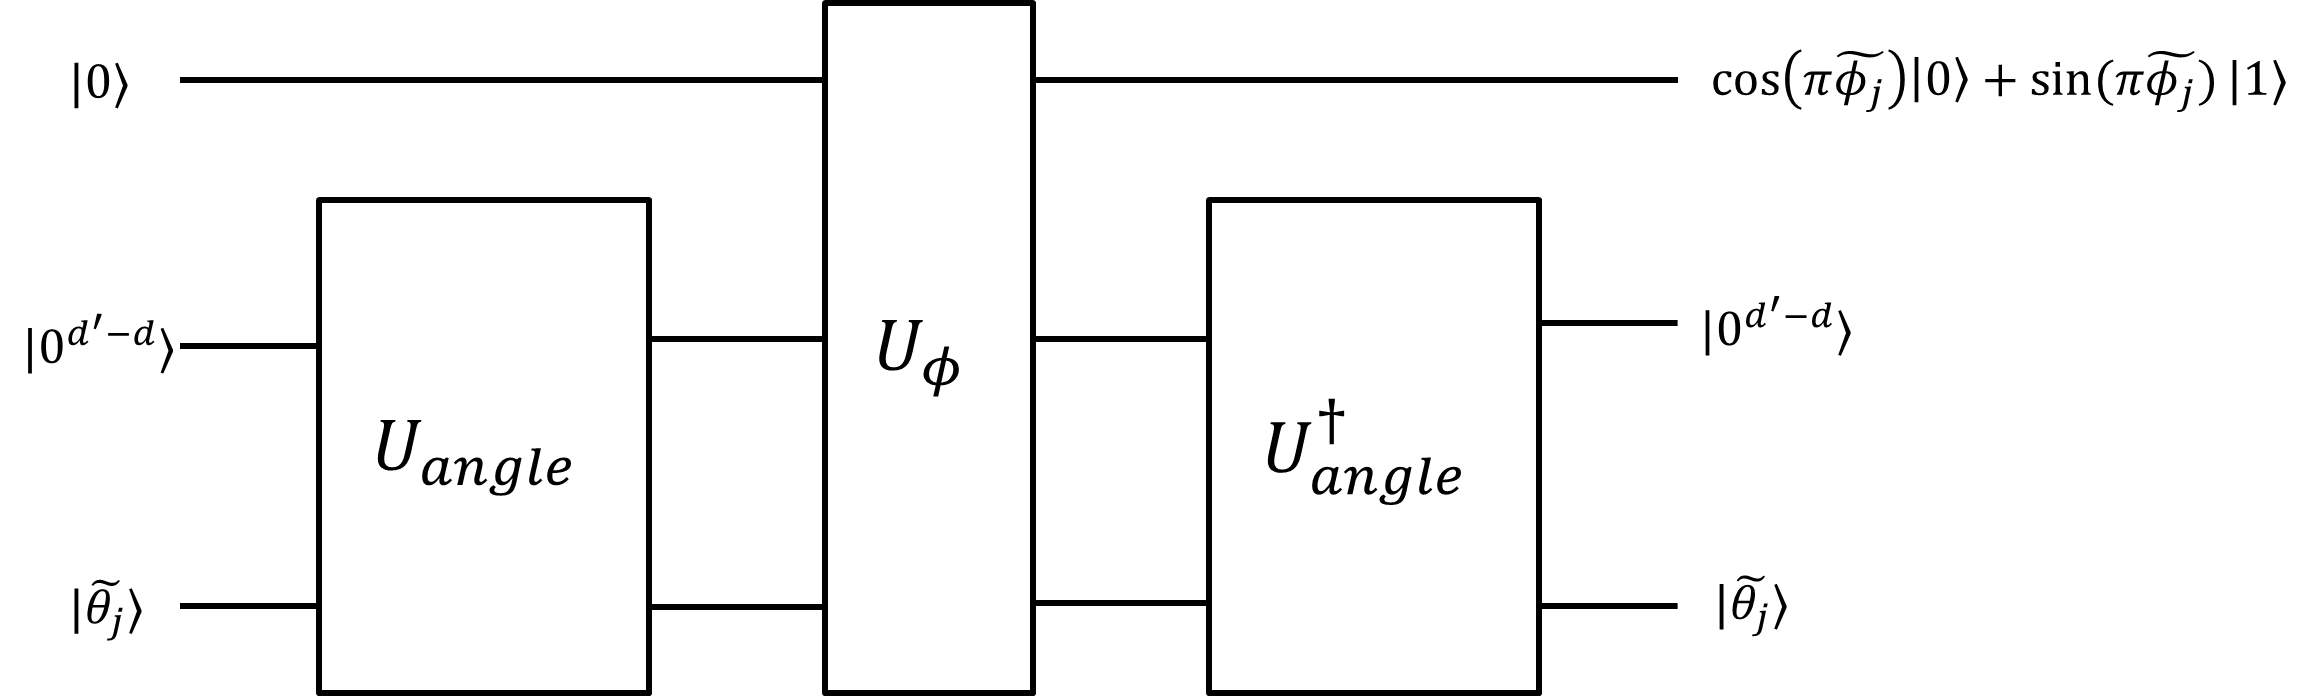
\includegraphics[width=\linewidth]{Images/Cr.png}
%         \caption{Entire Controlled Rotation}
%         \label{fig:cr}
%     \end{figure}
%     Therefore through the uncomputation $U_{angle}^{\dagger}$, the d'-d ancilla qubits also become a working register. Discard the working register we obtain a unitary $U_{CR}$ satisfying
%     \[
%     U_{CR}\ket{0}\ket{\tilde{\theta_j}}=(cos(\pi\tilde{\phi_j})\ket{0}+\sin (\pi\tilde{\phi_j})\ket{1})\ket{\tilde{\theta_j}}=\left(\sqrt{1-\frac{C^2}{\tilde{\theta'^2_j}}}\ket{0}+\frac{C}{\tilde{\theta_j'}}\ket{1}\right)\ket{\tilde{\theta_j}}
%     \]
%     This is the unitary circuit used in the HHL algorithm.
%     Now recall the state of the system after applying the QPE was
%     \[
%     \ket{0}\sum_{j=0}^{N-1}b_j\ket{\tilde{\theta_j}}\ket{\lambda_j}
%     \]
%     Thus, now we apply $U_{CR}$ to this state we get the following transformation:
%     \[
%     \ket{0}\sum_{j=0}^{N-1}b_j\ket{\tilde{\theta_j}}\ket{\lambda_j}\xrightarrow{U_{CR} \otimes I} \sum_{j=0}^{N-1} b_j \left(\sqrt{1-\frac{C^2}{\tilde{\theta^{'2}_j}}}\ket{0}+\frac{C}{\tilde{\theta_j'}}\ket{1}\right)\ket{\tilde{\theta_j}}\ket{\lambda_j}
%     \]
%     where each $\theta'_j \approx \lambda'_j$.
%     \item Finally, we perform uncomputation by applying $U^{\dagger}_{QPE}$, we convert the information from the ancilla register $\ket{\tilde{\theta_j}}$ back to $\ket{0}_{n_l}$. Thus, through the uncomputation, the $n_l$ ancilla qubits for storing the eigenvalues also becomes a working register. Discarding all the working registers, the resulting unitary denoted by $U_{HHL}$ satisfies
%     \[
%     U_{HHL}\ket{0}\ket{b}=\sum_{j=0}^{N-1} \left(\sqrt{1-\frac{C^2}{\tilde{\theta^{'2}_j}}}\ket{0}+\frac{C}{\tilde{\theta_j'}}\ket{1}\right)b_j\ket{\lambda_j}
%     \]
%     Finally, measuring the signal qubit, if the outcome is 1, we obtain the (unnormalized) vector
%     \[
%     \tilde{x}=\sum_j\frac{Cb_j}{\tilde{\theta'_j}}\ket{\lambda_j}
%     \]
%     stored as a normalized state in the system register is
%     \[
%     \ket{\tilde{x}}=\frac{\tilde{x}}{\|\tilde{x}\|}\approx \ket{x}
%     \]
%     which is the desired approximate solution to QLSP. In particular, the constant C does not appear in the solution.

%    \textbf{Recovering the norm of the solution: } The HHL algorithm returns the solution to QLSP in the form of a normalized state $\ket{x}$ stored in the quantum computer. In order to recover the magnitude of the unnormalized solution $\|\tilde{x}\|$, we note that the success probability of measuring the signal qubit in 1 is
%    \[
%    p(1)=\|\sum_j\frac{Cb_j}{\tilde{\theta'_j}}\|^2=\|\tilde{x}\|^2
%    \]
%    Therefore sufficient repetitions of running the circuit and estimate $p(1)$, we can obtain an estimate of $\|\tilde{x}\|$.
%     The general HHL circuit is as shown in the figure \ref{fig:hhl}.
%     \begin{figure}
%         \centering
%         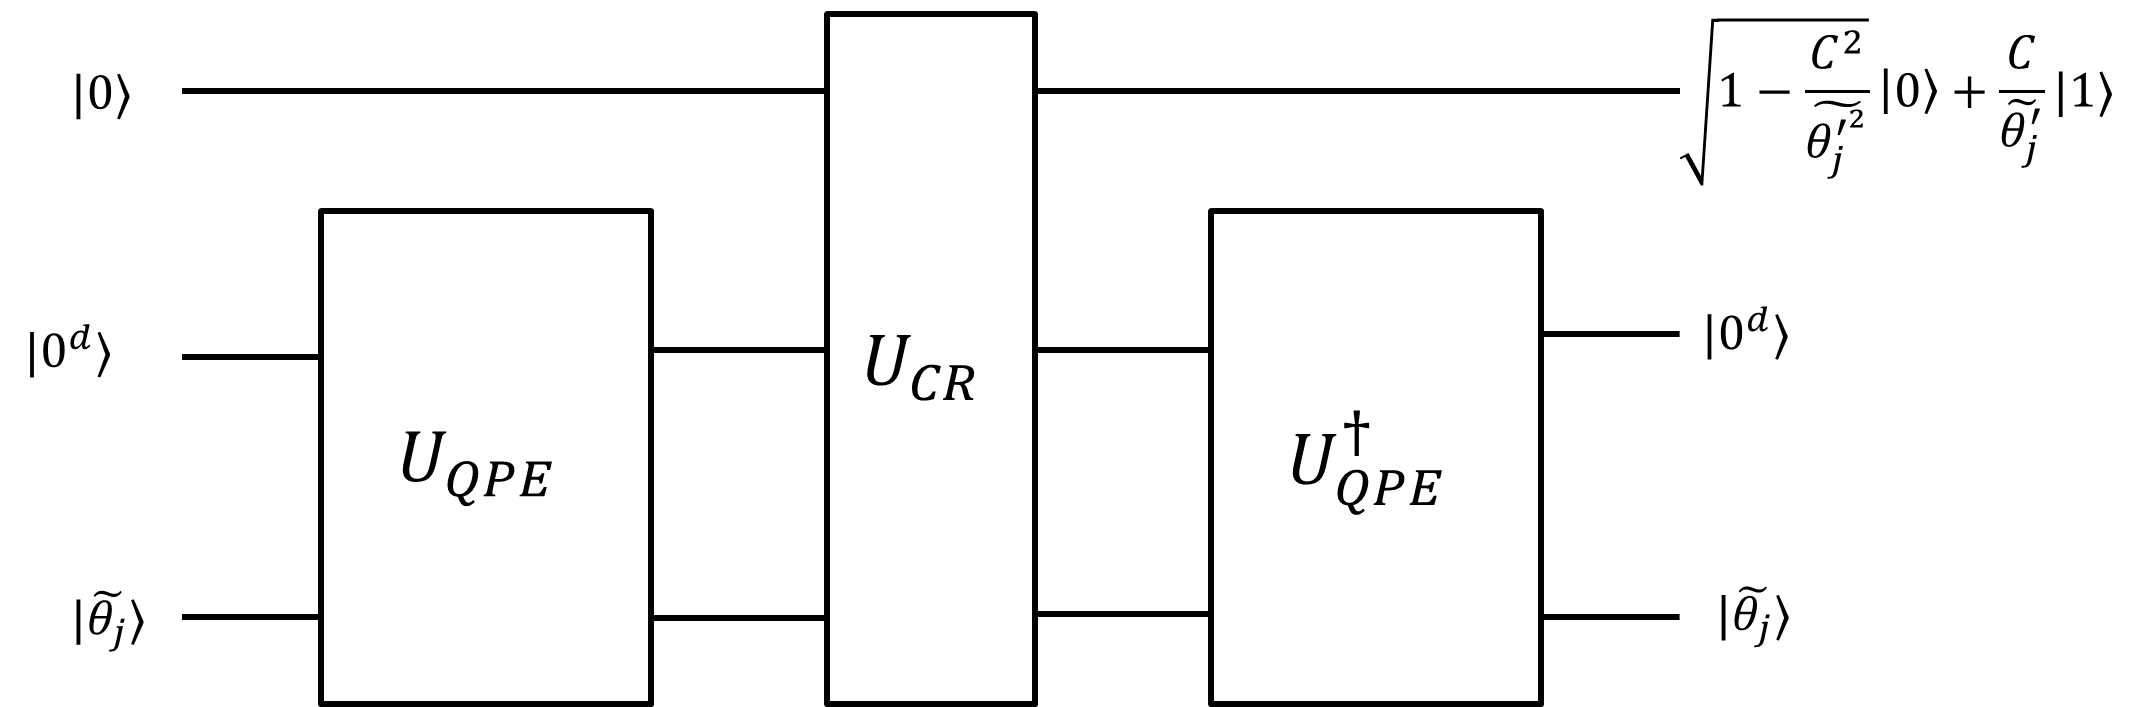
\includegraphics[width=\linewidth]{Images/Hhl.png}
%         \caption{HHL Circuit}
%         \label{fig:hhl}
%     \end{figure}
% \end{enumerate}
% \subsection{Example}
% \begin{example}
%     (4-qubit HHL) Consider an example to illustrate the algorithm. Consider
%     \[
%     A=\begin{bmatrix} 1 & -1/3 \\ -1/3 & 1 \end{bmatrix} \quad and \quad \ket{b}=\begin{bmatrix} 1 \\0 \end{bmatrix}
%     \]
%     Note that b is normalized and $b \in \mathbb{C}^2$. Thus, we need $n_b=1$ qubit to represent b. Also, $A \in \mathbb{C}^{2\times 2}$ is Hermitian, and hence will have two real eigen values ($\lambda_1,\lambda_2 \in \mathbb{R})$, thus we use $n_l=2$ qubits to store the binary representation of the eigen values and finally 1 auxiliary qubit for the conditioned rotation. Here, $N=2$.
%     \begin{enumerate}
%     \item We first prepare the state $\ket{b}$. Note that here in this example $\ket{b}=\ket{0}$, trivial.
%     \[
%     \ket{0}_{n_b} \xrightarrow{U_b} \ket{b}_{n_b}
%     \]
%     \item Now we apply QPE, with inputs as $\ket{b}_{n_b}$ and $\ket{0}_{n_l}$.
    
%     (Note that the eigen values of A are $2/3$ and $4/3$. and suppose we choose $t=3/8$, for simplicity. Thus, the eigen values of scaled A are: $(2/3)t = (2/3)(3/8) = 2/8=1/4=0.25=(0.01), (4/3)t=(4/3)(3/8)=4/8=1/2=0/5=(0.10)$, thus the eigen values of scaled A in binary are 0.01, 0.10. The corresponding eigen vectors of A are
%     \[
%     \ket{\lambda_1}=\frac{1}{\sqrt{2}}\begin{bmatrix} 1 \\ -1 \end{bmatrix} \quad and \quad \ket{\lambda_2}=\frac{1}{\sqrt{2}}\begin{bmatrix} 1 \\ 1 \end{bmatrix}
%     \]
%     Thus, we can write $\ket{b}$ in the eigen basis of A as
%     \[
%     \ket{b}_{n_b}=\frac{1}{\sqrt{2}}\left(\frac{1}{\sqrt{2}}\begin{bmatrix} 1 \\ -1 \end{bmatrix} \right) + \frac{1}{\sqrt{2}}\left(\frac{1}{\sqrt{2}}\begin{bmatrix} 1 \\ 1 \end{bmatrix} \right)=\frac{1}{\sqrt{2}}\ket{\lambda_1}+\frac{1}{\sqrt{2}}\ket{\lambda_2}
%     \]
%     $b_1=\frac{1}{\sqrt{2}},b_2=\frac{1}{\sqrt{2}}$.
%     \textbf{Note that all of this done here is not required since the algorithm will itself output the eigen values. This is done just for the sake of understanding and simplicity.})

%     Thus, QPE will output,
%     \[
%     \ket{0}\ket{0}_{n_l}\ket{b}_{n_b}\xrightarrow{I \otimes QPE} \ket{0}\sum_{j=0}^1b_j\ket{\tilde{\theta_j}}\ket{\lambda_j}=\frac{1}{\sqrt{2}}\ket{0}\ket{01}\ket{\lambda_!}+\frac{1}{\sqrt{2}}\ket{0}\ket{10}\ket{\lambda_2}
%     \]
%     \item Now we do controlled rotations. (Suppose we use $C=1/8$ that is less than the smallest (rescaled) eigen values of A i.e.$1/4$, recall, C should be chosen such that it is less than the smallest (rescaled) eigenvalue of $1/4$ but as large as possible so that when the auxiliary qubit is measured, the probability of being in the state $\ket{1}$ is large.)
%     Thus, as output of the controlled rotations we get,
%     \[
%     \ket{0}\sum_{j=0}^{N-1}b_j\ket{\tilde{\theta_j}}\ket{\lambda_j}\xrightarrow{U_{CR} \otimes I} \sum_{j=0}^{N-1} b_j \left(\sqrt{1-\frac{C^2}{\tilde{\theta^{'2}_j}}}\ket{0}+\frac{C}{\tilde{\theta_j'}}\ket{1}\right)\ket{\tilde{\theta_j}}\ket{\lambda_j}
%     \]
%     \begin{align*}
%         &=\frac{1}{\sqrt{2}}\left(\sqrt{1-\frac{(1/8)^2}{(1/4)^2}}\ket{0}+\frac{1/8}{1/4}\ket{1}\right)\ket{01}\ket{\lambda_1}+\frac{1}{\sqrt{2}}\left(\sqrt{1-\frac{(1/8)^2}{(1/2)^2}}\ket{0}+\frac{1/8}{1/2}\ket{1}\right)\ket{10}\ket{\lambda_2}\\
%     &=\frac{1}{\sqrt{2}}\left(\frac{\sqrt{3}}{2}\ket{0}+\frac{1}{2}\ket{1}\right)\ket{01}\ket{\lambda_1}+\frac{1}{\sqrt{2}}\left(\frac{\sqrt{15}}{4}\ket{0}+\frac{1}{4}\ket{1}\right)\ket{10}\ket{\lambda_2}\\
%     \end{align*}
%     \item Now we apply the uncomputation step $QPE^{\dagger}$, it will convert $\tilde{\theta_j}$ to $\ket{0}_{n_l}$,(thus discarding the working registers as they will not contribute anything now to the algorithm) we will get the final state of the system to be in,
%     \[
%     U_{HHL}\ket{0}\ket{b}=\sum_{j=0}^{N-1} \left(\sqrt{1-\frac{C^2}{\tilde{\theta^{'2}_j}}}\ket{0}+\frac{C}{\tilde{\theta_j'}}\ket{1}\right)b_j\ket{\lambda_j}
%     \]
%     Thus, the state of the system after the uncomputation will be:
%     \[
%     \frac{1}{\sqrt{2}}\left(\frac{\sqrt{3}}{2}\ket{0}+\frac{1}{2}\ket{1}\right)\ket{\lambda_1}+\frac{1}{\sqrt{2}}\left(\frac{\sqrt{15}}{4}\ket{0}+\frac{1}{4}\ket{1}\right)\ket{\lambda_2}
%     \]
%     Upon substituting, $\ket{\lambda_1}=\frac{1}{\sqrt{2}}\begin{bmatrix} 1 \\ -1 \end{bmatrix}= \frac{1}{\sqrt{2}}(\ket{0}-\ket{1})$\\$ \ket{\lambda_2}=\frac{1}{\sqrt{2}}\begin{bmatrix}1 \\ 1 \end{bmatrix} =\frac{1}{\sqrt{2}}(\ket{0}+\ket{1})$, we get,
%     \begin{align*}
%     &=\frac{1}{\sqrt{2}}\left(\frac{\sqrt{3}}{2}\ket{0}+\frac{1}{2}\ket{1}\right)\frac{1}{\sqrt{2}}(\ket{0}-\ket{1})+\frac{1}{\sqrt{2}}\left(\frac{\sqrt{15}}{4}\ket{0}+\frac{1}{4}\ket{1}\right)\frac{1}{\sqrt{2}}(\ket{0}+\ket{1}\\
%     &=\frac{\sqrt{3}}{4}\ket{00}-\frac{\sqrt{3}}{4}\ket{01}+\frac{1}{4}\ket{10}-\frac{1}{4}\ket{11}+\frac{\sqrt{15}}{8}\ket{00}+\frac{\sqrt{15}}{8}\ket{01}+\frac{1}{8}\ket{10}\\
%     &+\frac{1}{8}\ket{11}
%     \end{align*}
%     Thus, upon partial measurement of the auxiliary qubit (i.e. the first qubit here) to outcome 1, the state of the system will be:
%     \[
%     \frac{\frac{1}{4}\ket{10}-\frac{1}{4}\ket{11}+\frac{1}{8}\ket{10}+\frac{1}{8}\ket{11}}{\sqrt{\frac{5}{32}}}=\frac{\frac{3}{8}\ket{10}-\frac{1}{8}\ket{11}}{\sqrt{\frac{5}{32}}}=\ket{1}\otimes \frac{\frac{3}{8}\ket{0}-\frac{1}{8}\ket{1}}{\sqrt{\frac{5}{32}}}
%     \]
%     which is the value of normalized $\ket{x}$ in the second register. Thus,
%     \[
%     \frac{\ket{x}}{\|\ket{x}\|}=\frac{\frac{3}{8}\ket{0}-\frac{1}{8}\ket{1}}{\sqrt{\frac{5}{32}}}
%     \]
%     \item In order to calculate the norm of $\ket{x}$, we can perform several runs of the circuit and get the approximate $p(1)$. Here, the probability $p(1)$ we get,
%     \[
%     P(\ket{1})=\left(\frac{3}{8}\right)^2+\left(\frac{-1}{8}\right)^2=\frac{5}{32}=\|x\|^2
%     \]
%     In each of the run we can also measure the second register to get the approximate values of the components of x i.e. $p(0)\approx \left(\frac{3/8}{\sqrt{5/32}}\right)^2=\frac{9}{10}$ and $p(1)\approx \left(\frac{-1/8}{\sqrt{5/32}}\right)^2=\frac{1}{10}$. Thus, the components will be the root of the probabilities and then multiplying this by the norm to recover the components of the original vector x, we get,
%     \[
%     \sqrt{\frac{5}{32}}\left(\sqrt{\frac{9}{10}}\right)=\frac{3}{8}; \quad \sqrt{\frac{5}{32}}\left(\sqrt{\frac{1}{10}}\right)=\frac{1}{8}
%     \]
%     Now recall that we chose $t=3/8$ and $C=1/8$, hence the current x is the solution of $At$. Thus, in order to recover the original x, we are required to multiply $\frac{t}{C}$ to each of the components. Thus, we get,
%     \[
%     \frac{3/8}{1/8}\left(\frac{3}{8}\right)=\frac{9}{8}; \quad \frac{3/8}{1/8}\left(\frac{1}{8}\right)=\frac{3}{8}
%     \]
%     Thus, we get,
%     \[
%     x=\begin{bmatrix} 9/8 \\ 1/8 \end{bmatrix}
%     \]
%     Now, checking the value of x by substituting in $Ax$, we get,
%     \[
%     \begin{bmatrix} 1 & -1/3 \\ -1/3 & 1 \end{bmatrix} \begin{bmatrix} 9/8 \\ 3/8 \end{bmatrix}=\begin{bmatrix} 1 \\ 0 \end{bmatrix} =\ket{b}
%     \]
%     Thus, clearly, we have recovered the original solution x.
%     \end{enumerate}
%     \textbf{Note that here we multiply the components by $\frac{t}{C}$ can be explained as follows:
%     \begin{enumerate}
%         \item Multiplication by $\frac{1}{C}$, because recall that we are required to find 
%         \[
%         \ket{x}=\sum_{j=0}^{N-1}\lambda^{-1}_j b_j\ket{\lambda_j}
%         \]
%         but using the algorithm we obtained
%         \[
%         \ket{x}=\sum_{j=0}^{N-1}\lambda^{-1}_j C b_j\ket{\lambda_j}
%         \]
%         Thus, upon multiplying the components by $\frac{1}{C}$, we recover the original components. 
%         \item Multiplying by $t$: Recall that we are not finding the solution of $A$ but solution of scaled $A$ i.e. $At$.
%         \[At\ket{x'}=\ket{b}\]
%         Thus, the original solution will be $\ket{x}=t\ket{x'}$. Thus, the multiplication by t.
%     \end{enumerate}
%     Hence, upon multiplying the components of the square root of the approximate probabilities obtained from the algorithm by $\frac{t}{C}$, we recover the original components of x.
%     }
% \end{example}

% \section{Complexity Analysis}
% Recall that, in the final step of the algorithm we get,
% \[
% \tilde{x}=\sum_{j=0}^{N-1} \frac{Cb_j}{\tilde{\theta'_j}}\ket{\lambda_j}
% \]
% Thus, in the register it will be stored as:
% \[
% \ket{\tilde{x}}=\frac{\tilde{x}}{\|\tilde{x}\|} \approx \ket{x}
% \]
% We get the probability of getting outcome 1 is $p(1)$ as:
% \begin{align*}
% p(1) &= \|\tilde{x}\|^2=\|\sum_{j=0}^{N-1}\frac{Cb_j}{\tilde{\theta'}_j}\ket{\lambda_j}\|^2\\
% &=C^2\|\sum_{j=0}^{N-1}\frac{b_j}{\tilde{\theta'}_j}\ket{\lambda_j}\|^2\\
% &\approx C^2\|A^{-1}\ket{b}\|^2
% \end{align*}
% Therefore the success probability is determined by
% \begin{enumerate}
%     \item The choice of the normalization constant C
%     \item The norm of the true solution $\|x\|=\|A^{-1}\ket{b}\|$
% \end{enumerate}
% To maximize the success probability, $C$ should be chosen to be as large as possible (without exceeding $\lambda_0$). So assuming that the exact knowledge of $\lambda_0$, we can choose $C=\lambda_0$. For a Hermitian positive definite matrix A, (recall that 2-norm (induced norm is spectral norm) of any matrix A is given as $\|A\|_2=\sigma_{max}=\sqrt{\lambda_{max}(A^{\dagger}A)}$, thus, for a Hermitian matrix($A^{\dagger}=A; A=Q\Lambda Q^{\dagger} \implies \|A\|_2=\sqrt{\lambda_{max}(A^2)}= \sqrt{\lambda_{max}(Q\Lambda Q^{\dagger}Q\Lambda Q^{\dagger})}=\sqrt{\lambda_{max}(Q\Lambda^2Q^{\dagger})}=|\lambda_{max}|$ where $\lambda_{max}$ is the eigen value with the largest magnitude (irrespective of sign)) which is also positive definite (has all the eigen values $\geq 0$) A, $\|A\|=\lambda_{N-1}$, and $\|A^{-1}\|=\lambda^{-1}_0$. For simplicity, assume the largest eigenvalue of A is $\lambda_{N-1}=1$. Then the condition number of A is
% \[
% \kappa = \|A\|\|A^{-1}\|=\frac{\lambda_{N-1}}{\lambda_0}=C^{-1}
% \]
% Also, using the definition of norms ($\|A^{-1}\ket{b}\|\geq \|A^{-1}\|\|\ket{b}\|$)
% \[
% \|A^{-1}\ket{b}\|\geq \|A^{-1}\|\|\ket{b}\|=1
% \]
% Therefore, 
% \[
% p(1)=C^2\|A^{-1}\ket{b}\|^2\geq \frac{1}{\kappa^2}
% \]
% \[
% \implies p(1)=\Omega(\kappa^{-2})
% \]
% Thus, in the worst case we need to run the HHL algorithm for $\mathcal{O}(\kappa^2)$ times to obtain the outcome 1 in the signal bit.

% Assuming the number of qubits n is large, the circuit depth and the gate complexity of $U_{HHL}$ is mainly determined by those of $U_{QPE}$ because we assumed that it is easy to make $\ket{b}$ and the only other part in the circuit is controlled rotation which has less number of gates than QFT in QPE. Thus, the majority of circuit depth and gate complexity is dominated by QPE of the HHL circuit.
% Therefore we can measure the complexity of the HHL algorithm in terms of the number of queries to $U=e^{\iota 2\pi A}$. 

% In order to solve QLSP to precision $\epsilon$, we need to estimate the eigen values to multiplicative accuracy $\epsilon$ instead of the standard additive accuracy. \textbf{An $\epsilon$-additive precision is an algorithm that for a true solution $x$ returns $\tilde{x} \in [x-\epsilon,x+\epsilon$]. For a $\epsilon$-multiplicative precision algorithm, the algorithm returns $\tilde{x} \in [x(1+\epsilon),x(1-\epsilon)]$.} Assume $\tilde{\theta'_j}=\lambda_j(1+e_j)$ and $|e_j|\leq \frac{\epsilon}{4} \leq \frac{1}{2}$. Then the unnormalized solution satisfies
% \[
% \|\tilde{x}-x\|=\|\sum_j b_j\left(\frac{1}{\tilde{\theta'_j}}-\frac{1}{\lambda_j}\right)\ket{\lambda_j}\|\leq \|\sum_j\frac{b_j}{\lambda_j}\left(\frac{-e_j}{1+e_j}\right)\ket{\lambda_j}\|\leq \frac{\epsilon}{2}\|x\|
% \]
% Hence, using the property that $|\|\vec{x}\|-\|\vec{y}\||\leq \|\vec{x}+\vec{y}\|$
% \[
% |1-\frac{\|\tilde{x}\|}{\|x\|}|\leq \frac{\epsilon}{2}
% \]
% Then the normalized solution satisfies
% \[
% \|\ket{\tilde{x}}-\ket{x}\|=\|\frac{\tilde{x}}{\|\tilde{x}\|}-\frac{x}{\|x\|}\|\leq |1-\frac{\|\tilde{x}\|}{\|x\|}|+\frac{\|\tilde{x}-x\|}{\|x\|}\leq \epsilon
% \]
% The discussion requires the QPE to run to additive precision $\epsilon'=\lambda_0\epsilon=\epsilon/\kappa$. Therefore the query complexity of QPE is $\mathcal{O}(\kappa/\epsilon)$. Counting the number of times needed to repeat the HHl circuit, the worst case query complexity of the HHL algorithm is $\mathcal{O}(\kappa^3/\epsilon)$.

% The above ananlysis is the worst case analysis, because we assume $p(1)$ attains the lower bound $\Omega(\kappa^{-2})$. In practical applications, the result may not be so pessimistic. For instance, if $b_j$ centrates around the smallest eigen values of A, then we may have $\|x\|\approx \Theta(\lambda^{-1}_0=\Theta(\kappa^{-1})$. Then $p(1)=\Theta(1)$. IN such a case, we only need to repeat the HHl algorithm for a constant number of times to yield outcome 1 in the ancilla qubit. this does not reduce the query complexity of each run of the algorithm. Then in this best case, the query complexity is $\mathcal{O}(\kappa/\epsilon)$.

% \textbf{Additional Considerations: }Below we discuss a few more aspects of the HHL algorithm. The first observation is that the asymptotic worst-case complexity of the HHL algorithm can be generally improved using amplitude estimation.

% \begin{remark}
%     (HHL with amplitude amplification).
%     \[
%     U_{HHL}\ket{0}\ket{b}=\sqrt{p(1)}\ket{1}\ket{\psi_{good}}+\sqrt{1-p(1)}\ket{0}\ket{\psi_{bad}}, \quad \ket{\psi_{good}} = \ket{\tilde{x}}
%     \]
%     Since $\ket{\psi_{good}}$ is marked by a signal qubit, we may construct a signal qubit to construct a reflection operator with respect to the signal qubit. This is simply given by
%     \[
%     R_{good}=Z \otimes I_n
%     \]
%     The reflection with respect to the initial vector is
%     \[
%     R_{\psi_0}=U_{\psi_0}(2\ket{0{1+n}}\bra{0^{1+n}}-I)U^{\dagger}_{\psi_0}
%     \]
%     where $U_{\psi_0}=U_{HHL}(I_1\otimes U_b)$. Let $G=R_{\psi_0}R_{good}$ be the Grover iterate. Then amplitude amplification allows us to apply G for $\Theta(p(1)^{-\frac{1}{2}})$ times to boost the success probability of obtaining $\psi_{good}$ with constant success probability. Therefore in the worst case when $p(1)=\Theta(\kappa^{-2})$, the number of repetitions is reduced to $\mathcal{O}(\kappa)$, and the total runtime is $\mathcal{O}(\kappa^2/\epsilon)$. This query complexity is the commonly referred query complexity for the HHL algorithm. Note that as usual, amplitude amplification increases the circuit depth. However, the tradeoff is that the circuit depth increases from $\mathcal{O}(\kappa/\epsilon)$ to $\mathcal{O}(\kappa^2/\epsilon)$.
% \end{remark}
% So far our analysis, especially that based on QPE relies on the assumption that all $\lambda_j$ eigen values have exact d-bit representation. Such an assumption is unrealistic and causes theoretical and practical difficulties. Refer \cite{dervovic2018quantumlinearsystemsalgorithms} for a more detailed explanation.

% \begin{remark}
%     (Comparison with classical iterative linear system solvers). Let us now compare the cost of the HHL algorithm to that of classical iterative algorithms. If A is n-bit Hermitian positive definite with condition number $\kappa$, and is d-sparse (i.e. each row/column of A has at most d nonzero entries), then each matrix vector multiplication $Ax$ costs $\mathcal{O}(dN)$ floating point operations. The number of iterations for the steepest descent (SD) algorithm is $\mathcal{O}(\kappa\log \epsilon^{1})$, and this number can be significantly reduced to $\mathcal{O}(\sqrt{\kappa}\log \epsilon^{-1})$ by the renowned conjugate gradient (CG) method. Therefore the total cost (or wall clock time) of SD and CD is $\mathcal{O}(dN\kappa \log \epsilon^{-1})$ and $\mathcal{O}(dN\sqrt{\kappa}\log \epsilon^{-1})$, respectively.
% \end{remark}
% On the other hand, the query complexity of the HHL algorithm, even after using the Amplitude amplification algorithm, is still $\mathcal{O}(\kappa^2/\epsilon)$. Such a performance is terrible in terms of both $kappa$ and $\epsilon$. Hence the power of the HHL algorithm, and other QLSP solvers is based on that each application of A (in this case, using Unitary U) is much faster. In particular, if$U$ can be implemented with poly(n) gate complexity (also can be measured by the wall clock time), then the total gate complexity of the HHL algorithm (with Amplitude amplification) is $\mathcal{O}(poly(n)\kappa^2/\epsilon)$. When n is large enough, we expect that $poly(n)<<N=2^n$ and the HHL algorithm would eventually yield an advantage. Nonethelesss, for a realistic problem, the assumption that U can be implemented with $poly(n)$ cost should be taken with a grain of salt and carefully examined.

% \begin{remark}
%     (Readout problem of QLSP). By solving the QLSP, the solution is stored as a quantum state in the quantum computer, Sometimes the QLSP is only a subproblem of a larger application, so it is sufficient to treat the HHL algorithm (or other QLSP solvers) as a "quantum subroutine", and leave $\ket{x}$ in the quantum computer. However, in many applications (such as the solution of the Poisson's equation) the goal is to solve the linear system. Then the information in $\ket{x}$ must be recovered to a measurable classical output.

%     The most common case is to compute the expectation of some observable $\braket{\mathcal{O}}=\braket{x|\mathcal{O}|x}\approx \braket{\tilde{x}|\mathcal{O}|\tilde{x}}$. Assuming $\braket{\mathcal{O}}=\Theta(1)$. Then to reach additive precision $\epsilon$ of the observable, the number of samples needed is $mathcal{O}(\epsilon^{-2})$. On the other hand, in order to reach precision $\epsilon$, the solution vector $\ket{\tilde{x}}$ must be solved to precision $\epsilon$. Assuming the worst case analysis for the HHL algorithm, the total query complexity needed is
    
% \[
% \mathcal{O}(\kappa^2/\epsilon)\times \mathcal{O}(\epsilon^{-2})=\mathcal{O}(\kappa^2/\epsilon^3)
% \]

% \begin{remark}
%     (Query complexity lower bound). The cost of a quantum algorithm for solving a generic QLSP scales at least as $\Omega(\kappa(A))$ where $\kappa(A)=\|A\|\|A^{-1}\|$ is the condition number of $A$. The proof is based on converting the QLSP into a Hamiltonian simulation problem, and the lower bound with respect to $\kappa$ is proved via the no-fast-forwarding" theorem for simulating generic Hamiltonians \cite{harrow2009quantum}. Nonetheless, for speicific classes of hamiltonians, it may still be possible to develop fast algorithm to overcome this lower bound.
% \end{remark}

% \end{remark}

% \section{Improvements in HHL algorithm}
% The complexity of the above basic HHL algorithm can be improved further. Gilyen et al used the singular value transformation technique to implement $A^{-1}$, improving on an LCU construction due to Childs et al. We would like to apply the function $f(x)=1/x$ to a block-encoding of $A$ in order to get a block-encoding of $A^{-1}$ (up to normalization) that we can then apply to $\ket{b}\ket{0}$.

% The function $f(x)=1/x$ is not itself a polynomial, so we need to approximate it by a low-degree polynomial to be able to apply. Childs et al started from the following polynomial of degree $D=2b-1$ for $b=\mathcal{O}(\kappa^2 \log (\kappa/\epsilon))$:
% \[
% \dfrac{1-(1-x^2)^b}{x}
% \]
% This is indeed a polynomial because all terms in the numerator have degree $\geq 1$, so we can divide out the $x$ of the denominator. Since $(1-x^2)^b$ is close to $0$ (unless $|x|$ is small), this polynomial is indeed close to $1/x$ (unless $|x|$ is small, but we won't care about that because we'll apply this polynomial to a matrix whose eigenvalues aren't close to $0$). More precisely, this polynomial is $\epsilon/2$ close to $1/x$ whenever $x$ lies in the range $E_{\kappa}=[-1,-1/\kappa]\cup [1/\kappa,1]$. Its range on this domain is $[-\kappa,-1]\cup [1,\kappa]$ (ignoring the small $\epsilon$ for simplicity). Like every degree-$D$ polynomial, $f$ can be written exactly as a sum of $D+1$ Chebyshev polynomials of the first kind. These univariate polynomials are defined recursively as follows: $T_o(x)=1, T_1(x)=x$ and $T_{d+1}=2xT_d(x)-T_{d-1}(x)$. Note that $T_d$ has degree $d$, and maps $[-1,1]$ to $[-1,1]$. The polynomials $T_1,\ldots,T_D$ are linearly independent (even orthonormal in a certain way) and hence span the set of all univariate polynomials of degree $\leq D$. Childs et al show that the coefficients in this sum decrease quickly for larger degree, and that by dropping the resulting degree-$d$ polynomial $p$ $\epsilon$-approximates $1/x$ on the interval $E_k$, and its largest value (in absolute values) on this domain is $\kappa$. Now define the polynomial $P=p/(4\kappa)$. This has the same degree $d$ as $p$, but a range $[-1/4,1/4]$ that fits the assumption (there's a trick to ensure that the values of $P$ are within that range even for $x\approx 0$, which we'll skip here).
% We can implement a block-encoding of the $s$-sparse matrix $A/s$ using $O(1)$ sparse-access queries to $A$ and $O(n)$ other gates. Using a factor $O(s)$ more work, we can turn this into a block-encoding of $A$ itself (alternatively, we could directly invert the matrix $A/s$. whose singular values are $\geq 1/(\kappa s)$). With this block-encoding of $A$ and the polynomial $P=p/(4k)$, of degree $d=O(\kappa \log (\kappa/\epsilon))$. Note that all eigenvalues of $A$ lie in the interval $E_k$, where $p(x)\approx 1/x$, hence $p(A)\approx A^{-1}$ and $P(A)\approx \frac{1}{4\kappa}A^{-1}$. Then we have the block encoding of $P(A)$, at the expense of running the block-encoding of $A$ $O(d)$ times. Using $O(\kappa)$ rounds to amplitude amplification on top of this, we can get rid of the $1/(4\kappa)$ factor and end up with essentially the state $A^{-1}\ket{b}$ normalized. Note that we need to assume a unitary to prepare $\ket{b}$ here, having just one copy of $\ket{b}$ is not enough. We cannot use oblivious amplitude amplification because that assumes we have a block-encoding of a matrix that is proportional to a unitary (or close to that), which $A^{-1}$ is not. This gives a quantum algorithm that solves QLSP using $O(d\kappa s)=O(\kappa^2 s \log (\kappa/\epsilon))$ queries to $A$, and $O(\kappa s(\kappa n\log(\kappa/\epsilon)+B))$-2 qubit gates. Note that compared to basic HHL, dependence on $1/\epsilon$ has been improved from linear to logarithmic. The dependence on $\kappa$ can also be improved from quadratic to linear, using a technique called ``variable-time amplitude amplification".

% The HHL algorithm can in some cases solve the QLSP exponentially faster than classical algorithms can solve the LSP. In particular, if the sparsity $s$, the condition number $\kappa$, and the cost $B$ of preparing $\ket{b}$ are all $\leq polylog (N)$, and the allowed error is $\epsilon \geq 2^{-polylog(N)}$, then this improved version of the HHL algorithm uses $polylog(N)$ queries and gates to solve (in a quantum way) an $N$-dimensional linear system. It can also be used for other tasks, for instance approximately solving differential equations and other applications in scientific computing.
% \section{Implementation using Qiskit}

% \section{Applications}
% \subsection{Poisson's problem}
% Poisson's equation is a partial differential equation that describes the distribution of a potential field in a region. The equation is given as:
% \[
% \nabla^2 u+f=0
% \]
% where $u$ is the potential field, and $f$ is the source term. The Poisson's equation can be solved using the finite difference method. The finite difference method approximates the derivatives in the equation using finite difference schemes and discretizes the region into a grid, and the potential field is calculated at the grid points. The finite difference method converts the Poisson's equation into a linear system of equations, which can be solved using the HHL algorithm.
% Consider a toy problem of solving the Poisson's equation in one dimension with Dirichlet Boundary conditions as:
% \[
%     -u''(x)=f(x) \quad x \in [0,1] \quad u(0)=u(1)=0
% \]
% Using the central finite difference formula for discretizing the Laplacian operator on a uniform grid.
% \[
%     -\frac{\partial^2 u}{\partial x^2}=f(x) \quad x \in [0,1] \quad u(0)=u(1)=0
% \]
% Now recall that the central difference formula for discretizing second order derivative is
% \[
%     \frac{\partial^2 u}{\partial x^2} =\left(\frac{u_{i+1} -2u_{i} + u_{i-1}}{\Delta x^2}\right)
% \]
% Substituting in the equation we get the discretized form of the above Poisson's equation as:
% \[
%     -\left(\frac{u_{i+1} -2u_{i} + u_{i-1}}{\Delta x^2}\right)=f(x_i)
% \]
% Since we already know the solution at the boundary points from dirichlet conditions, thus, ignoring the values at the boundary points and writing equations at the N interior points we get,
% \[
% A=\frac{1}{h^2}\begin{bmatrix} 2 & -1 & 0 & \ldots & 0 & 0 & 0 \\ -1 & 2 & -1 &\ldots &0 & 0 & 0\\
% \vdots & \vdots & \ddots & \vdots & \vdots & \vdots & \vdots \\
% 0 & 0  & 0 &\ldots & -1 & 2 & -1 \\
% 0 & 0 & 0 & \ldots & 0 & -1 & 2 \\
% \end{bmatrix}
% \]
% where $h=\frac{1}{N+1}$, $x_i$ $\forall$ $i \in \{1,\ldots,N\}$. Let $u_i=u(x_i)$ and $f_i=f(x_i)$. We assume that vector $b$ is already normalized so that $\ket{f}=f$.

% \begin{proposition}
%     (Diagonalization of tridiagonal matrices) Consider the following Hermitian toeplitz tridiagonal matrix:
%     \[
%     A=\begin{bmatrix} a &\overline{b} &0 &\ldots & 0 & 0 & 0 \\
%     b & a & \overline{b} & \ldots & 0 & 0 & 0 \\
%     \vdots & \vdots & \vdots & \ddots & \vdots &\vdots &\vdots \\
%     0 & 0 & 0 & \ldots & b & a & \overline{b} \\
%     0 & 0 & 0 & \ldots & 0 & b & a\\
%     \end{bmatrix} \in \mathbb{C}^{N \times N}
%     \]
%     can be analytically diagonalized as
%     \[
%     Av_k=\lambda_kv_k, \quad k=1,\ldots,N.
%     \]
%     where $(v_k)_j=v_{j,k}$ denotes the jth component of $v_k$ eigen vector, $j=1,\ldots,N,b=|b|e^{\iota \theta}$, and
%     \[
%         \lambda_k=a+2|b| \cos \frac{k\pi}{N+1};\quad v_{j,k}=\sin \frac{jk\pi}{N+1}e^{\iota j\theta}
%     \]
% \end{proposition}
% \begin{proof}
%     Now $v_{j,k}=\sin \frac{jk\pi}{N+1}e^{\iota j\theta}$. Thus, note that $v_{0,k}=v_{N+1,k}=0$. Then direct matrix vector multiplication above shows that for any $j=1,\ldots, N$,
%     \[
%     (Av_k)_j=bv_{k,j-1}+av_{k,j}+\overline{b}v_{k,j+1}
%     \]
%     Upon substituting the value of $v_{k,j}$ we get,
%     \begin{align*}
%     (Av_k)_j&=b\sin \frac{(j-1)k\pi}{N+1}e^{\iota (j-1)\theta} + a \sin \frac{jk\pi}{N+1}e^{\iota j\theta} + \overline{b}\sin \frac{(j+1)k\pi}{N+1}e^{\iota (j+1)\theta}\\
%     &=a \sin \frac{jk\pi}{N+1}e^{\iota j\theta} + |b|e^{\iota  \theta}\sin \frac{(j-1)k\pi}{N+1}e^{\iota (j-1)\theta}+|b|e^{-\iota \theta} \sin \frac{(j+1)k\pi}{N+1}e^{\iota (j+1)\theta}\\
%     &=a\sin \frac{jk\pi}{N+1}e^{\iota j\theta} +|b|\left(\sin \frac{(j-1)k\pi}{N+1}+\sin \frac{(j+1)k\pi}{N+1}e^{\iota j\theta} \right)\\
%     &=a\sin \frac{jk\pi}{N+1}e^{\iota j\theta} +2|b|\sin\frac{jk\pi}{N+1} \cos \frac{k\pi}{N+1}e^{\iota j\theta}\\
%     &=\left(a+2|b|\cos \frac{k\pi}{N+1}\right) \sin \frac{jk\pi}{N+1}e^{\iota j\theta}\\
%     &=\lambda_k v_{j,k}\\
%     &=\lambda_k (v_{k})_j
%     \end{align*}
% \end{proof}
% Using this proposition and substituting with $a=2/h^2$, $b=-1/h^2$, the largest eigen value of A is $\lambda_{max}=\|A\|\approx \frac{4}{h^2}$, and the smallest eigen value $\lambda_{min}=\|A^{-1}\|^{-1} \approx \pi^2$. So,
% \[
% \kappa(A)=\|A\|\|A^{-1}\|\approx \frac{4}{h^2\pi^2} = \mathcal{O}(N^2)
% \]
% Recall that the circuit depth of the HHL algorithm is $\mathcal{O}(N^2/\epsilon)$, and the worst case query complexity (using AA) is $\mathcal{O}(N^4/\epsilon)$. So when N is large, there is little benefit in employing the quantum computer to solve this problem. 

% Let us now consider solving a d-dimensional Poisson's equation with Dirichlet boundary conditions
% \[
% -\nabla^2u(r)=b(r), \quad r=\Omega=[0,1]^d, \quad u|_{\partial \Omega}=0
% \]
% The grid is the Cartesian product of the uniform gird in 1D with N grid points per dimension and $h=1/(N+1)$. The total number of grid points is $N=N^d$. After discretization we will obtain a linear system $Au=b$, where
% \[
% A=A\otimes I \otimes I \ldots \otimes I + I \otimes A \otimes I \ldots \otimes I + \ldots + I \otimes I \ldots \otimes A
% \]
% where $I$ is the identity matrix of size N. Since A is Hermitian and positive definite, we have $\|A\|\approx 4d/h^2$, and $\|A^{-1}\|^{-1}=d\pi^2$. So $\kappa(A)\approx 4/(h^2\pi^2) \approx \kappa(A)$. There for the condition number is independent of the spatial dimension d.

% The worst case query complexity of the HHL algorithm is $\mathcal{O}(N^2/\epsilon)$. So when the number of grid points per dimension N is fixed and the spatial dimension d increases, and if $U=e^{\iota A\tau}$ can be implemented efficiently for some $\tau \|A\|<1$ with poly(d) cost, then the HHL algorithm will have an advantage over classical solvers, for which each matrix-vector multiplication scales linearly with N and is therefore exponential in d.

% \subsection{Solve Linear Differential Equations}
% Consider the solution of a time-dependent linear differential equation
% \[
% \frac{d}{dt}x(t)=A(t)x(t)+b(t), \quad t \in [0,T]
% \]
% \[
% x(0)=x_0
% \]
% Here $b(t),x(t) \in \mathbb{C}^d$ and $A(t) \in \mathbb{C}^{d \times t}$.
% The above differential equation can be used to represent a very large class of ordinary differential equations (ODEs) and spatially discretized partial differential equations (PDEs). For example, if $A(t)=-\iota H(t)$ for some Hermitian Matrix $H(t)$ and $b(t)=0$, this is the time-dependent Schrodinger equation
% \[
% \iota \frac{d}{dt}x(t)=H(t)x(t)
% \]
% A special case when $H(t)=H$ is often called the \textbf{Hamiltonian Simulation Problem}, and the solution can be written as
% \[
% x(T)=e^{\iota HT}x(0)
% \]
% which can be viewed as the problem of evaluating the matrix functions $e^{\iota HT}$.

% In this section we consider the general case, and for simplicity discretize the equation in time using  the forward Euler method with a uniform grid $t_k=k\Delta t$ where $\Delta t=T/N,k=0,\ldots, N$. Let $A_k=A(t_k),b_k=b(t_k)$. The resulting discretized system become
% \[
% x_{k+1}-x_k=\Delta t(A_kx_k+b_k), \quad k=1,\ldots,N
% \]
% \[
% x_{k+1}=(A_k\Delta t + I)x_k+b_k\Delta t
% \]
% \[
% x_{k+1}-(I + A_k\Delta t)x_k=b_k\Delta t
% \]
% \[
% -(I+A_k\Delta t)x_k+x_{k+1}=b_k\Delta t
% \]
% Note that for $t=0$, since we know that $x(0)=x_0$, thus the above equation reduces to
% \[
% x_1=(I+A_0\Delta t)x_0+\Delta tb_0
% \]
% which can be rewritten as
% \[\begin{bmatrix} I & 0 & 0 & \ldots & 0 & 0 \\
% -(I+\Delta tA_1) & I & 0 & \ldots &0 & 0\\
% 0 & -(I+\Delta tA_2) & I & \ldots & 0 & 0 \\
% \vdots & \vdots & \vdots & \ddots & \vdots & \vdots \\
% 0 & 0 & 0 & \ldots & -(I+\Delta tA_{N-1}) & I \end{bmatrix}
% \begin{bmatrix} x_1 \\x_2 \\x_3 \\ \vdots \\ x_N \end{bmatrix} =
% \begin{bmatrix} (I+\Delta t A_0)x_0+b_0\Delta t \\ b_1\Delta t\\b_2\Delta t\\ \vdots \\ b_{N-1}\Delta t \end{bmatrix}
% \]
% or more compactly as a linear system of equations
% \[
% \mathcal{A}x=b
% \]
% Here I is the identity matrix of size d, and $x \in \mathbb{R}^{Nd}$
% encodes the entire history of the states.

% To solve the equation as a QLSP, the right hand side b needs to be a normalized vector. This means we need to properly normalize $x_0,b_k$ so that
% \[
% \|b\|^2=\|(I+\Delta tA_0)x_0+\Delta tb_0\|^2+\sum_{k \in [N-1]} (\Delta t)^2\|b_k\|^2=1
% \]
% In the limit $\Delta t\rightarrow 0$, this can be written as
% \[\|b\|^2=\|x_0\|^2+\int_0^T \|b(t)\|^2 dt=1\]
% which is not difficult to satisfy as long as $x_0,b(t)$ can be prepared efficiently using unitary circuits and $\|x_0\|,\|b(t)\|=\Theta(1)$.

% To solve this equation using the HHL algorithm we need to estimate the condition number of $\mathcal{A}$. Note that $\mathcal{A}$ is a block-diagonal matrix and in particular is not Hermitian. So we need to use the dilation method and solve the corresponding Hermitian problem.

% \subsubsection{Scalar case} 
% In order to estimate the condition number, for simplicity we first assume $d=1$ (i.e., this is a scalar ODE problem), and $A(t)=a \in \mathbb{C}$ is a constant. Then
% \[
% \mathcal{A}=\begin{bmatrix} 1 & 0 & 0 & \ldots & 0 & 0\\
% -(1+a\Delta t) & 1 & 0 & \ldots & 0 & 0 \\
% 0 & -(1+a\Delta t) & 1 & \ldots & 0 & 0 \\
% \vdots & \vdots & \vdots & \ddots & \vdots & \vdots \\
% 0 & 0 & 0 & \ldots & -(1+a\Delta t) & 1 \end{bmatrix} \in \mathbb{C}^{N \times N}
% \]
% Recall that matrix $\mathcal{A}$ should be invertible. Thus, let $\zeta =1+a\Delta t$. When $Re(a)\leq 0$, the absolute stability condition of the forward Euler method requires $|1+a\Delta t|=|\zeta| < 1$. In general we are interested in the regime $\Delta t|a|<<1$, and in particular $|1+a\Delta t|=|\zeta|<2$.
% \begin{proposition}
%     For any $A \in \mathbb{C}^{N \times N},\|A\|^2,(1/\|A^{-1}\|)^2$ are given by the largest and smallest eigen values of $A^{\dagger}A$ respectively.
% \end{proposition}
%     We first need to compute
%     \[
%     \mathcal{A}^{\dagger}\mathcal{A}=\begin{bmatrix} 1+ |\zeta|^2 & -\overline{\zeta} & \ldots & \ldots & 0 & 0 \\ -\zeta & 1+|\zeta|^2 & -\overline{\zeta} & \ldots & 0 & 0\\
%     0 & -\zeta & 1+|\zeta|^2 & \ldots & 0 & 0 \\
%     \vdots & \vdots & \vdots & \ddots & \vdots & \vdots \\
%     0 & 0 & 0 & \ldots & 1+|\zeta|^2 & -\overline{\zeta} \\
%     0 & 0 & 0 & \ldots & -\zeta & 1 \end{bmatrix}
%     \]
% \begin{theorem} (Greshgorin Disk Theorem) Let $A \in \mathbb{C}^{N \times N}$ with entries $a_{ij}$. For each $i=1,\ldots,N$,define
%     \[
%     R_{i}=\sum_{j\neq i}|a_{ij}|
%     \]
%     Let $D(a_{ii},R_i) \subseteq \mathbb{C}$ be a closed disc centered at $a_{ii}$ with radius $R_i$, which is called a Greshgorin disk. Then every eigen value of A lies within at least one of the Greshgorin discs $D(a_{ii},R_i)$.
% \end{theorem}
% Since $\mathcal{A}^{\dagger}A$ is Hermitian, we can restrict the Greshgorin discs to the real line so that $D(A_{ii},R_i) \subseteq \mathbb{R}$. Then Greshgorin discs of the matrix $\mathcal{A}^{\dagger} \mathcal{A}$ satisfy the bound
% \[
% D(a_{11},R_1)\subseteq [1+|\zeta|^2-|\zeta|,1+|\zeta|^2+|\zeta|]
% \]
% \[
% D(a_{ii},R_i)\subseteq[1+|\zeta|^2-2|\zeta|,1+|\zeta|^2+2|\zeta|], \quad i=2,\ldots,N-1
% \]
% \[
% D(a_{NN},R_N)\subseteq [1-|\zeta|,1+|\zeta|]
% \]
% Now using the proposition we have, for $D(a_{ii},R_i)\subseteq[1+|\zeta|^2-2|\zeta|,1+|\zeta|^2+2|\zeta|], \quad i=2,\ldots,N-1$. Thus, the maximum eigen value is
% \[
% \lambda_{max}(\mathcal{A}^{\dagger}\mathcal{A})\leq (1+|\zeta|)^2<9
% \]
% for all values of $a$ such that $|\zeta|<2$.

% To obtain a meaningful lower bound of $\lambda_{min}(\mathcal{A}^{\dagger}\mathcal{A})$, we need $Re(a)<0$ and hence $|\zeta|<1$. Use the inequality
% \begin{align*}
% \sqrt{1+x} &\leq 1+\frac{1}{2}x, \quad x>-1\\
% \implies -\sqrt{1+x} &\geq -1-\frac{1}{2}x, \quad x>-1\\
% \implies 1-\sqrt{1+x} &\geq -\frac{1}{2}x. \quad x>-1
% \end{align*}
% we have
% \[
% 1-|\zeta|=1-\sqrt{(1+\Delta tRe(a))^2+(\Delta t)^2(Im(a))^2}\geq -\frac{1}{2}((\Delta t)^2(Re(a))^2+2Re(a)\Delta t+(\Delta t)^2(Im(a))^2)
% \]
% \[
% 1-|\zeta|\geq -Re(a)\Delta t-\frac{1}{2}(\Delta t)^2|a|^2 \geq -\frac{\Delta t}{2} Re(a)
% \]
% when $(\Delta t)^2|a|^2<(-\Delta t Re(a))$ is satisfied. Then we have
% \[1>1-|\zeta|\geq -\frac{\Delta t}{2}Re(a)\]
% Now using the proposition we have, for $D(a_{ii},R_i)\subseteq[1+|\zeta|^2-2|\zeta|,1+|\zeta|^2+2|\zeta|], \quad i=2,\ldots,N-1$. Thus, the minimum eigen value is
% \[
% \lambda_{min}(\mathcal{A}^{\dagger}\mathcal{A})\geq (1-|\zeta|)^2\geq \frac{(\Delta t Re(a))^2}{4}
% \]
% Therefore
% \[
% \|A\|=\sqrt{\lambda_{max}(\mathcal{A}^{\dagger}\mathcal{A})}\leq \sqrt{1+|\zeta|^2+2|\zeta|}<3
% \]
% and
% \[
% \|A^{-1}\|^{-1}=\sqrt{\lambda_{min}(\mathcal{A}^{\dagger}\mathcal{A})}\geq\frac{\Delta t(-Re(a))}{2}
% \]
% As a result, when $(-Re(a))=\Theta(1)$, the condition number satisfies
% \[
% \kappa(\mathcal{A})=\|\mathcal{A}\|\|\mathcal{A}^{-1}\|=\mathcal{O}(1/\Delta t)
% \]
% In summary, for the scalar problem $d=1$ and $Re(a)<0$, the query complexity of the HHL algorithm is $\mathcal{O}((\Delta t)^{-2}\epsilon^{-2})$.
% \begin{remark}
%     It may be tempting to modify the $(N.N)$ th entry of $\mathcal{A}$ to be $1+|\zeta|^2$ to obtain
%     \[
%     \mathcal{G}=\begin{bmatrix} 1+ |\zeta|^2 & -\overline{\zeta} & 0 & \ldots & 0 & 0 \\ -\zeta & 1+|\zeta|^2 & -\overline{\zeta} & \ldots & 0 & 0\\
%     0 & -\zeta & 1+|\zeta|^2 & \ldots & 0 & 0 \\
%     \vdots & \vdots & \vdots & \ddots & \vdots & \vdots \\
%     0 & 0 & 0 & \ldots & 1+|\zeta|^2 & -\overline{\zeta} \\
%     0 & 0 & 0 & \ldots & -\zeta & 1+|\zeta|^2 \end{bmatrix}
%     \]
%     Here $\mathcal{G}$ is a Toeplitz tridiagonal matrix satisfying the requirements of Proposition 7.7.1. The eigen values of $\mathcal{G}$ take the form
%     \[
%     \lambda_k=1+|\zeta|^2+2|\zeta|\cos \frac{k\pi}{N+1};\quad k=1,\ldots,N
%     \]
%     If we take the approximation $\lambda_{min}(\mathcal{A}^{\dagger}\mathcal{A})\approx \lambda_{min}(\mathcal{G})$, we would find that the above equation holds even when $Re(a)>0$. This behavior is however incorrect, despite that the matrices $\mathcal{A}^{\dagger}\mathcal{A}$ and $\mathcal{G}$ only differ by a single entry!
% \end{remark}

% \subsubsection{Vector Case}
% Here we consider a general $d>1$, but for simplicity assume $A(t)=A \in \mathbb{C}^{d \times d}$ is a constant matrix. We also assume $A$ is diagonalizable with eigenvalue decomposition
% \[
% A=V\Lambda V^{-1}
% \]
% and $\Lambda=diag(\lambda_1,\ldots,\lambda_N)$. We only consider the case $Re(\lambda_k) < 0$ for all $k$.
% \begin{proposition}
%     For any diagonalizable $A \in \mathbb{C}^{N \times N}$ with eigenvalue decomposition $Av_k=\lambda v_k$, we have
%     \[
%     \|A^{-1}\|^{-1}\leq \min_k|\lambda_k|\leq \max_k|\lambda_k|\leq \|A\|
%     \]
% \end{proposition}
% \begin{proof}
%     Use the Schur form $A=QTQ^{\dagger}$, where $Q$ is an unitary matrix and $T$ is an upper triangular matrix. The diagonal entries of $T$ encodes all eigenvalues of $A$, and the eigenvalues can appear in any order along the diagonal of $T$. The proposition follows by arranging the eigenvalue of $A$ with the smallest and largest absolute values to the (N,N)th entry, respectively. 
% \end{proof}

% The absolute stability condition of the forward Euler method requires $\Delta t\|A\|<1$, and we are interested in the regime $\Delta t\|A\|<<1$. Therefore $\Delta t|\lambda_k|<<1$ for all k. Let I be the identity matrix of size d, and denote $B=-(I+\Delta tA)$, then
% \[
% \mathcal{A}^{\dagger}\mathcal{A}=\begin{bmatrix} I + B^{\dagger}B & B & \ldots & 0 & 0 & 0 \\ B & I + B^{\dagger}B & B^{\dagger} & \ldots & 0 & 0 \\
% \vdots & \vdots & \vdots & \ddots &\vdots & \vdots  \\
% 0 & 0 & 0 & \ldots & I+B^{\dagger}B & B^{\dagger} \\
% 0 & 0 & 0 & \ldots & B & I \end{bmatrix}
% \]
% Note that
% \[
% \|B\|\leq \|I+B^{\dagger}B\|\leq 1+(1+\Delta t\|A\|)^2\leq 5
% \]
% For any $x\in\mathbb{C}^{Nd}$,
% \[
% \|A^{\dagger}Ax\|^2 \leq \|I+B^{\dagger}B\|[(\|x_1\|^2+\|x_2\|^2)+(\|x_1\|^2+\|x_2|^2+\|x_3\|^2)+\ldots(\|x_{N-1}\|^2+\|x_N\|^2)]\leq 15\|x\|^2
% \]
% So $\lambda_{max}(A^{\dagger}A)\leq 15$, and
% \[
% \|A\|=\sqrt{\lambda_{max}(A^{\dagger}A)}\leq\sqrt{15}=\mathcal{O}(1)
% \]
% To bound $\|A^{-1}\|$, we first note that from the eigenvalue decomposition of $A$, we have
% \[
% A=\begin{bmatrix}
%     V & & & \\
%     & V & & \\
%     & & \ddots & \\
%     & & & V
% \end{bmatrix}
% \begin{bmatrix}
%     I & 0&0&\ldots &0 & 0 \\
%     -(I+Delta t\Lambda) & I & 0 & \ldots & 0& 0 \\
%     0 & -(I+\Delta t\Lambda) & I & \ldots & 0 & 0 \\
%     \vdots & \vdots &\vdots & \vdots & \vdots &\vdots \\
%     0 & 0 & 0 &ldots & -(I+\Delta t \Lambda) & I 
% \end{bmatrix}
% \begin{bmatrix}
%     V^{-1} & & & \\& V^{-1} & & \\ & & & \ddots & \\ & & & & V^{-1}
% \end{bmatrix}
% \]
% Hence $\kappa(V)=\|V\|\|V^{-1}\|$ is the condition number of the eigenvector matrix
% \[
% A_k=\begin{bmatrix}
%     1 & 0 & 0 & \ldots &0 & 0 \\-(1+\Delta t\lambda_k) & 1 & 0 & \ldots & 0 & 0 \\
%     \vdots & \vdots & \vdots &\vdots &\vdots &\vdots \\
%     0 & 0 & 0 & \ldots & -(1+\Delta t\lambda_k) & 1 
% \end{bmatrix}
% \]
% This reduces the problem to the scalar case. Let $\zeta_k=1+\Delta t\lambda_k$, and assume
% \[
% Re\lambda_k <0, \Delta t|\lambda_k|<(-Re\lambda_k)/|\lambda_k|, \forall k
% \]
% then, we have
% \[
% \min_k \|A_k^{-1}\|^{-1}\geq \frac{\Delta t\min_k(-Re\lambda_k)}{2}
% \]
% So if $\min_k (-Re\lambda_k)=\Theta(1)$, we have
% \[
% \kappa(A)=\mathcal{O}(\kappa(V)/\Delta t),
% \]
% and the cost of the HHL algorithm is $\mathcal{O}((\Delta t)^{-2}\epsilon^{-2}\kappa(V))$. Hence compared to the scalar case, the condition number of the eigenvector matrix $V$ can play an important role.

% \subsection{Computing observables}
% The solution means that the normalized state $\ket{x}$ is computed to precision $\epsilon$ and stored in the quantum computer. In order to evaluate observables at the final time $T$, i.e., $\bra{x(T)}O\ket{x(T)}$, we find that by the normalization condition, $\|x(T)\|$ is on average $\mathcal{O}(N^{-\frac{1}{2}})=\mathcal{O}((\Delta t)^{\frac{1}{2}})$, and $\bra{x(T)}O\ket{x(T)}=\mathcal{O}(\Delta t)$. Therefore instead of reaching accuracy $\epsilon$, the Monte Carlo procedure must reach precision $\mathcal{O}(\epsilon\Delta t)$. This increases the number of samples by another factor of $\mathcal{O}((\Delta t)^{-2})$.

% There is however a simple way to overcome this problem. Instead of solving the equations, we can reduce $x$ by artificially padding the vector with $N$ copies of the final state $x_N$. This can be written as and can be reinterpreted as
% \[
% \mathbf{X}=\ket{0}\otimes x+\ket{1}\otimes y
% \]
% with the unnormalized vector 
% \[
% x=\begin{bmatrix}
%     x_1\\x_2\\\vdots\\ x_N
% \end{bmatrix}, y=\begin{bmatrix}
%     x_{N+1}\\x_{N+2}\\ \vdots \\ x_{2N}
% \end{bmatrix}=\begin{bmatrix}
%     x_N\\ x_N \\ \vdots \\ x_N
% \end{bmatrix}
% \]
% and the corresponding linear system of equation becomes
% \[
% \begin{bmatrix}
%     I & & & & & & \\
%     -(I+\Delta tA_1) & I  &&& \\
%     &&\ddots&&&&& \\
%     &&-(I+\Delta tA_{N-1}) & I &&&&\\
%     &&&-I & I&&& \\
%     &&&&-I & I &&\\
%     &&&&&&\ddots & \\
%     &&&&&&-I & I 
% \end{bmatrix}
% \begin{bmatrix}
%     x_1\\x_2\\\vdots \\ x_N \\ x_{N+1}\\x_{N+2}\\\vdots \\ x_{2N}
% \end{bmatrix}=\begin{bmatrix}
%     (I+\Delta tA_0)x_0+\Delta tb_0\\ \Delta tb_1\\ \vdots \\ \Delta tb_{N-1}\\ 0 \\ 0 \\ \vdots \\ 0
% \end{bmatrix}
% \]
% Note that the solution vector only requires one ancilla qubit, after solving the equation. The condition number of this modified equation is still $\mathcal{O}((\Delta t)^{-1})$, so the total query complexity is $\mathcal{O}((\Delta t)^{-2}\epsilon^{-2})$. By solving the modified equation to precision $\epsilon$, we can estimate $\bra{x(T)}O\ket{x(T)}$ by
% \[
% \bra{y}I\otimes O\ket{y}
% \]
% of which the magnitude does not scale with $\Delta t$. Here $i$ is the identity matrix of size $N$, and $y$ can be obtained by measuring the ancilla qubit and obtain $1$. If the norm of $\|x(t)\|$ is comparable for all $t\in[0,T]$, then the success probability will be $\Theta91)$ after $\ket{X}$ is obtained.

% \begin{example}
%     \textbf{(The heat equation)} As an application of the differential equation solver, let us consider a toy problem for solving the heat equation in one-dimension with Dirichlet boundary conditions
%     \[
%     \partial_t u(r,t)=u''(r),\quad r\in\Omega=[0,1],\quad u(0t)=u(1,t)=0
%     \]
%     After spatial discretization using the central finite difference method with $d$ grid points, this becomes a linear ODE system
%     \[
%     \partial_t u=-Au
%     \]
%     where $Ain\mathbb{R}^{N\times N}$ is a tridiagonal matrix. After applying the forward Euler method and discretize the simulation time $T$ and $L$ intervals with $\Delta t=T/L$, we obtain a linear system of size $NL$. The eigenvalues of $-A$, denoted by $\lambda_k$, are all negative and satisfy
%     \[
%     -\frac{4}{h^2}\approx -\|A\|\leq \lambda_k\leq -\|A^{-1}\|^{-1}\approx-\frac{1}{\pi^2}
%     \]
%     the absolute stability condition requires $|1+\Delta t\lambda_k|<1$,or $\Delta t<h^2/4=\mathcal{O}(N^{-2})$, which impleis $L=\mathcal{O}(N^2)$. Since $A$ is Hermitian, we have $\kappa(V)=1$. so for $T=\mathcal{O}(1)$, the query complexity for solving the heat equation is $\mathcal{O}(N^2\epsilon^{-2})$, which is the same as solving Poisson;s equation.

%     Again, the potential advantage of the quantum solver only appears when solving the $d$-dimensional heat equation
%     \[
%     \partial_t u(r,t)=\Delta u(r), \quad r\in\Omega=[0,1]^d,\quad u(,t)|_{d\Omega}=0
%     \]
%     This can be written as a linear system of equations
%     \[
%     \partial_t u=-Au,
%     \]
%     where $A$ is given as before. The eigenvalues are all negative. Note that $\|A\|=\Theta(dN^2)$, then $h=\mathcal{O}(d^{-1}N^{-2})$, and the query complexity of the HHL solver is $\mathcal{O}(dN^2\epsilon^{-2})$. This could potentially have an exponential advantage over classical solvers.
% \end{example}






% \chapter{Quantum Walk Algorithms}
% Quantum walks have been shown to have computational advantages over classical random walks. 

% In the calssical setting, a particle starts out in some initial position (vertex) on a graph $H=(V,E)$ and ``walks" to neighboring vertices in a probabilistic manner; these are classical random walks. the final probability distribution of finding the particle at a given vertex $V$ - as well as question such as ``hoe long does it take the particle to reach a particular vertex?" - are interesting and useful quantitites to calculate. When certain problems are phrased in terms of random walks, for example the 2-SAT problem, computing these quantitites can lead to novel slutions that may not have been known previously.

% The simplest example of a classical random walk is a one-dimensional walk on a line. Consider a particle starting at position $x(t=0)=0$ at time $t=0$. At time $t=1$, the particle moves to the right $(x(1)=1)$ or left $(x(t=1)=-1)$ with equal probability. At time $t=2$, we have $x(2)=x(1)\pm 1$ with equal probability, and in general $x(t)=x(t-1)\pm 1$ with equal probability. Because steps are made at only discrete increments of time $t=1,2,3,\ldots,$ this is known as a discrete-time random walk. Continuous time random walks are another model which we discuss below.

% Classical random walks are implemented by generating psuedo-random number(s) at each time step. The particle's position is updated at each iteration according to the outcome of the random number generator. Alternatively, an array of values representing probabilities for each position can be stored and updated via a stochastic matrix which determines the time evolution of the system.

% Quantum walk is one of the major topics in quantum algorithms. A Quantum Walk (QW) is the quantum version of classical random walk, which has found a lot of algorithmic applications. We begin by discussing classical random walks and study concepts of fundamental to their operation, such as Markov chains. Then we develop their quantum counterpart, quantum walks, and discuss how they try to mimic random walks in a way that takes advantage of their quantum features for speedup. This lecture will be more of a survey of the general concepts and applications of quantum walks. Roughly speaking, there are two versions of quantum walks. The continuous time quantum walk is closely analogous to its classical counterpart, i.e. continuous time random walk. The other version, the discrete time quantum walk, or Szegedy's quantum walk is not so obviously connected to the classical random walks. We will introduce motivations behind the continuous and discrete time random walks.

% \section{Discrete-time quantum walk}
% In the case of a discrete-time quantum walk on a line, the idea is similar but the implementation is different. The quantum walk consists of two registers of qubits: a position register $P$ and a coin register $C$. As the name suggests the position register tracks the probability distribution for the particle to be at a particular position $\ket{0},\ket{1},\ldots,\ket{N-1}$, where we impose periodic boundary condition $\ket{N}=0$. The coin register is used to update the particle's position at each time step.

% The update to the particle's position is given by the shift operator
% \[
% S=\ket{0}\bra{0}_C \otimes \sum_i \ket{i-1}\bra{i}_P + \ket{1}\bra{1}_C \otimes \sum_i {i+1}_p\bra{i}_P
% \]
% That is, if the coin register is in the state $\ket{1}$ state, the particle shifts to the left, and if the coin register is in the state $\ket{0}$ state, the particle shifts to the right. That is,
% \[
% S\ket{0}_C\otimes \ket{i}_P = \ket{0}_C\otimes \ket{i-1}_P
% \]
% and
% \[
% S\ket{1}_C\otimes \ket{i}_P = \ket{1}_C\otimes \ket{i+1}_P
% \]
% The coin is ``flipped" by applying a single qubit gate - for example the Hadamard gate $H$ to produce an equal superposition state, though ``biased coins can also be made - and then the shift operator is applied. One step of the quantum walk algorithm can be written
% \[
% U = S(H_C\otimes I_P)
% \]
% where $H_C$ is the Hadamard acting on the coin and $I_P$ refers to the identity acting on the particle. $T$ steps of the walk are given by $U^T$.

% In this simplest example of a random walk, numerous differences between the classical and quantum cases can already be seen. For example, starting in the initial state $\ket{0}_C\otimes \ket{0}_P$ will cause the probability distribution to drift ``to the left" -that is, the particle is more likely to move to the left - whereas in the classical case the distribution is symmetric. Starting the quantum walk in the state $\ket{1}_C\otimes \ket{0}_P$ will cause the distribution to drift to the right. The reasons for this are constructive and destructive interference of amplitudes, a distinctly quantum phenomena that is not possible in the classical case. Note that the distribution for quantum walk can be made symmetric - by starting in the state $\ket{+}_C\otimes \ket{0}_P$, for example, where $\ket{+}=(\ket{0}+\ket{1})/\sqrt{2}$.

% The simplest example is instructive for understanding both how quantum walks work and how quantum walks are different than classical walks. Upon further study, more differences can be seen. For example, the variance of the classical distribution for a discrete-time random walk on a line is $\sigma_C^2 =T$ after $T$ time steps, but in the quantum case it is $\sigma_C^2=T^2$. Thus, the quantum walker propagates quadratically faster than the classical one.







% \section{Random Walk}
% \subsection{Setup}
% A graph is a set of points called vertices connected by lines called edges. Each edge $(u,v)$ will have a weight $w$, which is proportional to the probability of moving to vertex $v$ when currently at vertex $u$. We only consider finite undirected graphs $G=(V,E)$ where $V$ denotes the set of $N=n(V)$ vertices, and $E$ denotes the set of edges.

% We can represent the weighted graph as a symmetric function $w:V\times V\rightarrow [0,\infty)$, where each possible edge can exist between two vertices gets mapped to a weight ranging from $0$ to infinity. The edges that are in $V \times V$ but not in $E$ have weights equal to zero (i.e., for $x\in V\times V$ and $x\notin E$, $w(x)=0)$; therefore, $E$ has nonnegative edge weights.

% The undirected nature of $G$ is reflected in the symmetry of $w$ with respect to the two vertices that it connects: $w(u,v)=w(v,u)$.

% The weight of a vertex $u\in C$ is defined as the sum of the weights of all incident edges on $u$:
% \[
% w(u)=\sum_{v \in V} w(u,v)
% \]
% We assume that name of the vertices in $G$ is isolated. In the unweighted setting, this means that every vertex is connected to at least one other vertex. In general, this indicates $w(u)>0$ for each $u\in V$.

% \subsection{Process}
% A random walk is a process that starts by picking a starting vertex from an initial probability distribution $\sigma$ of $V$. In each step it moves from the current vertex $u\in V$ to a neighboring vertex $v\in V$ with a probability proportion to $w(u,v)$. When the graph is unweighted, the subsequent vertex that the walk moves to is picked uniformly at random among the neighbors of the current vertex. This process is repeated for a number of steps. We are interested in how the probability distribution evolves as the number of steps increases. This process can be modeled with Markov chains, which we will cover next.

% \section{Markov Chain}
% One way to model and analyze the behavior of a random walk is by viewing it as a Markov chain. this is a memory less stochastic process, where the probability distribution of the next step depends on the current state, and retains no history of the past steps to arrive at where you are.

% \subsection{Transition Matrix}
% The probability distribution obtained from a Markov chain can be described by a transition matrix $T$, which is an $N\times N$ matrix with components defined as follows:
% \[
% T_{vu}=Pr[\text{move to v |at u}]=\frac{w(u,v)}{w(u)}
% \]
% The transition matrix $T$ can be used to describe the probability distribution after $t$ steps of the random walk as $T^t\sigma$, i.e., as the product of the $t$-th power of $T$ with a column vector representing the initial probability distribution $\sigma$. The column vector has one component for every vertex $v$, equal to the probability of being at $v$. The transition matrix $T$ is symmetric ($T_{uv}=T_{vu}$ for all $u,v\in V$) iff $w(u)=w(v)$ for all $u,v\in V$i.e., iff the weight $w(u)$ of every vertex $u$ is the same. For unweighted graphs, $T$ is symmetric iff the degree of every vertex is the same, i.e., the graph $G$ is regular.

% \subsection{Stationary distribution}
% If a Markov chain converges to some distribution, that distribution needs to be stationary i.e., invariant under $T$.

% There may be multiple stationary distributions, but the following distribution $\pi$ always is one:
% \[
% \pi(v)=\frac{w(v)}{W}, \quad \text{where } W=\sum_v w(v)
% \]
% \begin{proof}
%     When the current distribution is $\pi$, the weight that is sent from $u$ to $v$ in one step of the random walk equals $T_{vu}\cdot \pi(u)$. Rewriting this expression, we get the following:
%     \[
%     T_{uv}\cdot \pi(u)=\frac{w(u,v)}{w(u)}\cdot \frac{w(u)}{W}=\frac{w(u,v)}{W}
%     \]
%     Since $w$ is symmetric in $u$ and $v$ (i.e., $w(u,v)=w(v,u)$), the weight sent from $u$ to $v$ equals the weight sent from $v$ to $u$, which gives us the following result:
%     \[
%     \frac{w(u,v)}{W}=\frac{w(v,u)}{W}=\frac{w(v,u)}{w(v)}\cdot \frac{w(v)}{W}=T_{uv}\cdot \pi(v)
%     \]
%     Thus, the probability at the vertex $v$ after the stochastic matrix $T$ acts on the stationary distribution $\pi$ is given as:
%     \[
%     p(v)=\sum_u T_{vu}\cdot \pi(u)=\sum_u \frac{w(u,v)}{W}=\frac{1}{W}\sum_uw(u,v)
%     \]
%     Since $w$ is symmetric in $u$ and $b$, the above expression simplifies to
%     \[
%     p(v)=\frac{1}{W}\sum_u w(v,u)=\frac{w(v)}{W}=\pi(v)
%     \]
%     Thus, the probability distribution $\pi$ is a stationary distribution.
% \end{proof}

% \begin{corollary}
%     Note that $\pi$ is uniform ff $w(u)$ is independent of $u$ iff $T$ is symmetric. In particular, in the unweighted case, $\pi$ is uniform iff the graph $G$ is regular.
% \end{corollary}

% As a side note, a Markov chain that has a stationary distribution $\sigma$ with the property that $T_{vu}\cdot\sigma(u)=T_{uv}\cdot\sigma(v)$ is called reversible; random walks on undirected graphs are equivalent to reversible Markov chains.

% \section{Convergence Analysis}
% We restrict to an important case where $T$ is symmetric; if that is the case, we can do a spectral analysis of $T$ to analyze the convergence of the markov chain to a stationary distribution $\pi$. In the general case, one uses the discriminant matrix $D$ defined as:
% \[
% D_{uv}=\sqrt{T_{uv}\cdot T_{vu}}
% \]
% Note that $D$ is always symmetric, and that $D=T$ iff $T$ is symmetric.
% \subsection{Spectrum of T}
% Since $T$ is a symmetric real matrix, all its eigenvalues are real. Moreover, the eigenvalues have absolute values at most $1$.

% \begin{proof}
%     Since $T$ is stochastic, for any vector $x$
%     \[
%     \|Tx\|_1=\sum_v|\sum_{u}T_{vu}x_u|\leq \sum_u|x_u|\sum_v T_{vu}=\sum_u |x_u |=\|x\|_1
%     \]
%     If $\lambda$ is an eigenvalue fo $T$ with corresponding eigenvector $x$, then $|\lambda|\|x\|_1=\\|\lambda x\|_1=\|Tx\|_1$, which implies that $|\lambda|\leq 1$.
% \end{proof}

% The eigenvalue $1$ of $T$ represents invariance, so there always is an eigenvector of $1$, namely corresponding to the invariant distribution $\pi$. The multiplicity of the eigenvalue $1$ equals the number of connected components of $G$. This means that there is a unique stationary distribution iff $G$ is connected. In addition, $T$ has an eigenvalue $-1$ iff $G$ is bipartite. Thus, this leads to the following conclusion:
% \begin{corollary}
%     With the exception of the stationary distribution $pi$, all eigenvectors of $T$ have eigenvalues strictly less than $1$ in absolute value iff $G$ is connected and non-bipartite.
% \end{corollary}
% We are going to use these facts in our convergence analysis of the stationary distribution $\pi$.

% \subsection{Convergence Analysis for Symmetric $T$}
% As a symmetric matrix, $T$ has an orthogonal basis of eigenvectors including $\pi$. Then every vector, which is the distribution at any point in time throughout the random walk, can be described as a linear combination of these eigenvectors. Note that the component of any distribution $\sigma$ along $\pi$ equals $\pi$. This is because the inner product
% \[
% (\sigma,\pi)=\frac{1}{N}\sum_{u\in V}\sigma(u)=\frac{1}{N}
% \]
% is independent of $\sigma$. It follows that $(\sigma-\pi,\pi)=0$, so that $\sigma-\pi$ has no component along $\pi$.

% To check for convergence to $\pi$, we want to bound the difference between the distribution after $t$ steps of the random walk, and the stationary distribution $\pi$. Since we know that $\sigma-\pi$ is orthogonal to $\pi$ we can expand $\sigma-\pi$ in the set of all orthogonal eigenvectors $\beta_i$ of $T$ excluding $\pi$. That is to say there exist coefficients $c_i$ such that
% \[
% \sigma-\pi=\sum_i c_i\beta_i,\beta_i\neq \pi,\forall i \implies T^t(\sigma-\pi)=\sum_i c_iT^t\beta_i
% \]
% \[
% T^t(\sigma-\pi)=\sum_i c_iT^t\beta_i \implies \|T^t(\sigma-\pi)\|_2^2 =\|\sum_i c_i \lambda_i^t \beta_i \|_2^2 = \sum_i |c_i|^2 |\lambda_{i}|^{2t}
% \]
% Here we have used the fact that $\|\alpha a+\beta b\|^2=|\alpha|^2\|a\|^2+|\beta|^2 \|b\|^2$ when $a$ and $b$ are orthogonal. Since, $\|\beta_i\|=1\forall i$. The above equation thus simplifies to 
% \[
% ||T^t(\sigma-\pi)\|_2^2 \leq \lambda_{max}^{2t} \sum_i |c_i|^2 =\lambda_{max}^{2t} \|\sigma-\pi\|_2^2
% \]
% Note that the 1-norm of $\pi$ is equal to $1$, from which you can show that the 2-norm of $\sigma-\pi$ is at most $1$:
% \[
% \|\pi\|_1 =1=\|\pi-\sigma+\sigma\|_1
% \]
% In order to bound the statistical distance between the two distribution we use the Cauchy-Schwarz inequality to upper bound the $1$-norm as a function of the $2$-norm:
% \[
% \|x\|_1 = \sum_i |x_i|=(X,\hat{1})\leq \|X\|_2 \|\hat{1}\|_2 =\|X\|_2 \sqrt{N}=\|x\|_2 \sqrt{N}
% \]
% Now, using the fact that $\|\cdot\|_2\leq \|\cdot \|_1$, we get,
% \begin{align*}
% \|\pi-\sigma+\sigma\|_2^2 &\leq 1\\
% \|\sigma-\pi\|_2^2+\|\sigma\|_2^2&\leq 1\\
% \|\sigma-\pi\|_2^2&\leq 1-\|\sigma\|_2^2
% \end{align*}
% Here, we have used the fact that $\|\sigma-\pi\|$ and $\|\pi\|$ are orthonormal vectors. Since, $\|\sigma\|_2^2$ is always positive, the above simplifies to,
% \[
% \|\sigma-\pi\|_2^2\leq 1
% \]
% Therefore, we have that
% \[
% \|T^t\sigma-\pi\|_2^2=\|T^t\sigma-T^t\pi\|_2^2 = \|T^t(\sigma-\pi)\|_2^2 \leq \lambda_{max}^{2t} \|\sigma-\pi\|_2^2
% \]
% Using the above results, we arrive at the conclusion
% \[
% \|T^t\sigma-\pi\|_2 \leq \lambda_{max}^{t} \|\sigma-\pi\|_2 \leq \lambda_{max}^{t}
% \]
% where $\lambda_{max}$ denotes the maximum absolute value of an eigenvalue corresponding to an eigenvector that is orthogonal to $\pi$: $\lambda_{max}=\max \{|\lambda|:\text{(eigenvalue with eigenvector)}\perp \pi\}$. This gives us an upper bound on how far the distribution after $t$ steps of the Markov chain is from the stationary distribution $\pi$.

% We can express this upper bound in terms of spectral gap $\delta$, where $\delta =1-\lambda_{max}$, as follows:
% \[
% \lambda_{max}^{t} =(1-\delta)^{t} \leq exp(-\delta)^{t} =exp(-\delta t)
% \]
% where we used the fact that $1+x\leq exp(x)$ for $x=-\delta$; this follows from the convexity of the exponential function. Thus,
% \[
% \|T^t\sigma-\pi\|_2\leq (1-\delta)^t\leq exp(-\delta t)
% \]
% Hence, using the result that $\|\cdot\|_1\leq \sqrt{N}\|\cdot\|_2$, we get, 
% \[
% \|T^t\sigma-\pi\|_1\ \leq \sqrt{N}\|T^t\sigma-\pi\|_2 \leq \sqrt{N}\lambda_{max}^t \leq \sqrt{N}exp(-\delta t)
% \]
% Thus, we can guarantee that $\|T^t\sigma-\pi\|_1 \leq \eta$ by setting $t\geq \frac{1}{\delta}\ln (\sqrt{N}/\eta)$.

% Convergence to $\pi$ is guaranteed as long as $\delta >0$, which is the case iff $G$ is connected and non-bipartite. The number of steps required to approach $\pi$ scales as $1/\delta$. If we want to guarantee fast convergence, we need a large spectral gap $\delta$. On the other hand, if $\delta$ is close to zero, convergence may be slow.


% \section{Classical Random Walks}
% Consider an undirected graph $G$ with $N$ vertices. Suppose at least an $\epsilon$- fraction of the vertices are ``marked", and we would like to find a marked vertex. One way to do this is with a random walk:
% \begin{enumerate}
%     \item Start at some specific vertex $y$ of the graph.
%     \item Repeat the following a number of times. 
%     \item Check if $y$ is marked, and if not then choose one of its neighbors at random and set $y$ to be that neighbor.
% \end{enumerate}
% This may seem like a stupid algorithm, but it has certain advantages. For instance, it only need space $\mathcal{O}(\log N)$, because you need to keep track of the current vertex $y$ (Say there are 8 vertices then they can be represented using 3 bits, thus $\log N$ space required to keep track of the current vertex), and maybe a counter that keeps track of how many steps you have already taken. Note that here we are assuming the neighbors of a given vertex are efficiently computable, so you don't actually need to keep the whole graph in memory. This will be true for all graphs we consider here. Such an algorithm can for example decide whether there is a path from specific vertex $y$ to a specific vertex $x$ using $\mathcal{O}(\log N)$ space. We'd start the walk at $y$ and only $x$ would be marked; one can show that if there exists a path from $y$ to $x$ in G, then we will reach $x$ in $poly(N)$ steps.

% let us restrict attention to $d$-regular graphs without self-loops, so each vertex has exactly $d$ neighbors. A random walk on such a graph $G$ corresponds to an $N \times N$ symmetric matrix $P$, where $P_{x,y} = 1/d$ if $(x,y)$ is an edge in $G$, and $P_{x,y}=0$ otherwise. This $P$ is the normalized adjacency matrix of $G$. If $v \in \mathbb{R}^N$ is a vector with a $1$ at position $y$ and 0s elsewhere, then $Pv$ is a vector whose $x$-th entry is $(Pv)_x=1/d$ if $(x,y)$ is an edge, and $(Pv)_x=0$ otherwise. In other words, $Pv$ is the uniform probability distribution over the neighbors of $y$, which is what you get by taking on step of the random walk starting at $y$. More generally, if $v$ is a probability distribution on the vertices, then $Pv$ is the new probability distribution on the vertices after taking one step of the random walk, and $P^kv$ is the probability distribution after taking $k$ steps.

% Suppose we start with some probability-distribution vector $v$ (which may or may not be centered at one vertex $y$). We will assume $G$ is connected and not bipartite. Then $P^kv$ will converge to the uniform distribution over all vertices, and the speed of convergence is determined by the ``gap" between the first eigenvalue of $P$ and all the other eigenvalues. This can be seen as follows. Let $\lambda_1 \geq \lambda_2 \geq \ldots \geq \lambda_N$ be the eigenvalues of $P$, ordered by size, and $v_1, v_2, \ldots, v_N$ be corresponding orthogonal eigenvectors. (Analysing graphs by looking at the eigenvalues and eigenvectors of their adjacency matrix is called ``algebraic graph theory" or ``spectral graph theory". The largest eigenvalue is $\lambda_1=1$, and corresponds to eigenvector $v_1=u=(1/N)$ which is the uniform distribution over all vertices. One can show that our assumption that $G$ is connected implies $\lambda_2 < 1$, and our assumption that $G$ is not bipartite implies $\lambda_N > -1$. Hence all eigenvalues $\lambda_i$ $\forall i \in \{2,\ldots,N\}$ will be in $(-1,1)$; the corresponding eigenvector $v_i$ will be orthogonal to the uniform vector $u$, so the sum of its entries is $0$. Let $\delta > 0$  be the difference between $\lambda_1 = 1$ and $\max_{i\geq 2}|\lambda_i|$ (hence $|\lambda_i|\leq 1-\delta$ for all $i \geq 2$). This $\delta$ is called the ``spectral gap" of the graph.

% Now decompose the starting distribution $v$ as $v =\sum_{i=1}^N \alpha_i v_i$. Since the sum of $v$'s entries is $1$, and the sum of $v_1$'s entries is $1$, while each other eigenvector $v_i$ ($i\geq2$) has entries summing to $0$, it follows that $\alpha_1=1$. Now let us see what happens if we apply the random walk for $k$ steps, starting from $v$:
% \[
% P^kv=P^k\left(\sum_i \alpha_i v_i\right) =\sum_i \alpha_i \lambda_i^kv_i =u+\sum_{i\geq 2}\alpha_i\lambda_i^k v_i
% \]
% Consider the squared norm of the difference between $P^kv$ and $u$:
% \begin{align*}
% \|P^kv-u\|^2 = \left\|\sum_{i\geq 2} \alpha_i\lambda_i^k v_i\right\|^2 = \sum_{i\geq 2}|\alpha_i|^2 |\lambda_i|^{2k} &\leq \sum_{i\geq 2}|\alpha_i|^2 (1-\delta)^{2k}\\
% &\leq (1-\delta)^{2k}\sum_{i\geq 2}|\alpha_i|^2\\
% &\leq (1-\delta)^{2k}\sum_i |\alpha_i|^2\\
% \|P^{k}v-u\|^2&\leq \|v\|^2(1-\delta)^{2k}
% \end{align*}
% Since $v$ is a probability distribution we have $\|v\|^2\leq 1$. By choosing $k=ln(1/\eta)/\delta$, we get $\|P^kv-u\|\leq \eta$. In particular, if $\delta$ is not too small, then we get quick convergence of the random walk to the uniform distribution $u$, no matter which distribution $v$ started with (convergence in total variation distance can be derived from this by Cauchy-Schwarz, choosing $\eta <<1/\sqrt{N}$). Once we are close to the uniform distribution, we have probability roughly $\epsilon$ of hitting a marked vertex.Of course, the same happens if we just pick a vertex uniformly at random, but that may not always be an option if the graph is given implicitly.

% Suppose it costs $S$ to set up an initial state $v$; it costs $U$ to update the current vertex i.e. to perform one step of the random walk; and it costs $C$ to check whether a given vertex is marked. ``Cost" is left undefined for now, but typically it will count the number of queries to some input, or number of elementary operations. Consider a classical search algorithm that starts at $v$, and then repeats the following until it finds a marked vertex: check if the current vertex is marked, and if not run a random walk for roughly $1/\delta$ steps to get close to the uniform distribution. Ignoring constant factors, the expected cost before this procedure finds a marked item, is on the order of
% \[
% S+\frac{1}{\epsilon}\left(C + \frac{1}{\delta}U\right)
% \]
% \section{Applications of Random Walks}
% Random walks can be used to model real world phenomena; for instance, in physics they are used as simple models of Brownian motion. They also can be used to model gambling. In this section we review two of the most common applications in computer science: sampling and search. We focus a little more on search, as our study of quantum walks is focus on their applications in search.

% \subsection{Sampling}
% This is the most common use of classical random walks. If we want to sample from a complicated distribution $\pi$, we can set p a random walk with stationary distribution $\pi$, start from a simple distribution $\sigma$ (e.g. a point distribution), and run the random walk for a number of steps. If the spectral gap $\delta$ is large, then a small number of steps suffice to bring us close to $pi$. This is known as rapid mixing. If the underlying graph is simple, the process yields an efficient way to (approximately) sample from $\pi$.

% The process may also be of interest in case $\pi$ is simple, say uniform, but one cannot obtain a uniform sample as a primitive. In such settings expander graphs are often helpful. These are infinite families of graphs that have bounded (i.e. ,constant) degree and a spectral gap $\delta$ that is at least some positive constant. by the above analysis, regular expanders exhibit rapid mixing to the uniform distribution, so small number of steps of a random walk starting from some fixed vertex suffices to obtain an almost-uniform sample.

% \subsection{Search}
% Another application that is perhaps less common classically, but it is very important in the quantum setting, is search.

% Assume we have a set $V$ of vertices, some of which are good and others bad, and our goal is to find a good vertex. As before, we represent goodness as a Boolean function $f:V\rightarrow \{0,1\}$, where $f(v)=1$ indicates that $v$ is good. One way to search for a good vector is to pick one uniformly at random, and check whether $f$ evaluates to one. If so, we are done if not, we retry. If the fraction $\epsilon$ of good vertices is large, we expect we only need a few trials until the first success, namely $1/\epsilon$. However, similar to the above sampling setting, obtaining a vertex may be expensive. Instead of picking a uniform sample for each trial, it may be cheaper to move to a neighboring vertex in the underlying graph $G$, and use that for our next trial. In such settings, searching for a good vertex using a random walk makes sense.

% We distinguish between three contributions to cost of this search process: setup, update and check.

% \begin{itemize}
%     \item 
%     Setup cost $S$: The cost of picking a sample from the start distribution $\sigma$, which may or may not be the stationary distribution $\pi$. We incus this cost each time we start the random walk.
%     \item Update cost $U$: The cost to execute one step of the random walk. We will incur this cost $t$ times when we perform a random walk of length $t$.
%     \item Check cost $C$: The cost to determine whether the current vertex $v$ is good, i.e., whether$f(v)=1$. We may or may not want to do this for every step of the random walk.
% \end{itemize}


% \section{Introduction to Quantum Walks}
% Let $G=(V,E)$ be a graph of size $N$. A Markov chain (or a random walk) is given by a transition matrix $P$, with its entry $P_{ij})$ denoting the probability of the transition from vertex $i$ to vertex $j$. The matrix $P$ is a stochastic matrix satisfying
% \[
% P_{ij}\geq 0,\quad \sum_j P_{ij}=1
% \]
% A Markov chain is irreducible if any state can be reached from any other state in a finite number of steps. An irreducible Markov chain is aperiodic if there exists no integer greater than one that divides the length of every directed cycle of the graph. A Markov chain is ergodic if it is both irreducible and aperiodic. By the Perron-Frobenious Theorem, any ergodic Markov chain $P$ has a unique stationary state $\pi$, and $\pi_i>0$ for all $i$. A Markov chain is reversible if the following detailed balance condition is satisfied
% \[
% \pi_iP_{ij}=\pi_jP_{ji}
% \]
% Now we define the discriminant matrix associated with a Markov chain as
% \[
% D_{ij}=\sqrt{P_{ij}P_{ji}}
% \]
% which is real symmetric and hence Hermitian. For a reversible Markov chain, the stationary state can be encoded as an eigenvector of $D$.

% \begin{proposition}
%     (Reversible Markov chain). If a Markov chain is reversible, then the coherent version of the stationary state
%     \[
%     \ket{\pi}=\sum_i \sqrt{\pi_i}\ket{i}
%     \]
%     is a normalized eigenvector of the discriminant matrix $D$ satisfying
%     \[
%     D\ket{\pi}=\ket{\pi}
%     \]
%     Furthermore, when $\pi_i>0$ for all $i$, we have
%     \[
%     D=\text{diag}(\sqrt{\pi})P\text{diag}(\sqrt{\pi})^{-1}
%     \]
%     therefore the set of (left) eigenvalue of $P$ and the set of the eigenvalues of $D$ are the same.
% \end{proposition}

% \subsection{Block encoding of the discriminant matrix}
% Our first goal is to construct a Hermitian block encoding of $D$. Assume that we have access to an oracle $O_p$ satisfying
% \[
% O_p\ket{0^n}\ket{j}=\sum_k \sqrt{P_{jk}}
% \]
% Thanks to the stochasticity of $P$, the right hand side is already normalized vector and no additional signal qubit is needed.

% We also introduce the n-qubit SWAP operator SWAP operator:
% \[
% SWAP\ket{i}\ket{j}=\ket{j}\ket{i}
% \]
% which swaps the value of the two registers in the computational basis, and can be directly implemented using $n$-two qubit SWAP gates.

% We claim that the following circuit gives $U_D\in HBE_{1,n}(D)$
% \begin{figure}
%     \centering
%     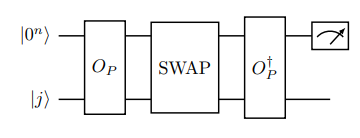
\includegraphics[width=0.5\linewidth]{Images/qwalkcirc.png}
%     \caption{Circuit for the Hermitian block encoding of a discriminant matrix}
%     \label{fig:qwalencD}
% \end{figure}
% \begin{proposition}
%     Figure \ref{fig:qwalencD} defines $U_D\in HBE_{1,n}(D)$.
% \end{proposition}
% \begin{proof}
%     Clearly $U_D$ is unitary and Hermitian. Now we compute as before
%     \[
%     \ket{0^n}\ket{j}\xrightarrow{O_P}\sum_k \sqrt{P_{jk}}\ket{k}\ket{j}\xrightarrow{SWAP}\sum_K \sqrt{P_{jk}}\ket{j}\ket{k}
%     \]
%     So the inner product gives
%     \[
%     \bra{0^n}\bra{i}U_D\ket{0^n}\ket{j}=\sum_{k,k'}\sqrt{P_{ik'}P_{jk}}\delta_{j,k'}\delta_{i,k}=\sqrt{P_{ij}P_{ji}}=D_{ij}
%     \]
%     This proves the claim.
% \end{proof}

% \section{Quantum Walk}
% \subsection{Discrete-time Quantum Walk}
% We like to setup an iterative process just like the classical walk that allows us to mimic a classical random walk, but in such a way that we move faster. Quantum walks take advantage of the quantum phenomenon of interference to speed up the convergence.

% \subsubsection{Model}
% For ease of exposition we consider the unweighted symmetric case. Now, if we are at vertex $v$m we would like to have a unitary transformation (quantum operations are unitary) that maps a vertex $v$ to a uniform superposition of the neighbors of $v$.
% \[
% \ket{v}\rightarrow \ket{N_v}=\frac{1}{\sqrt{|N_v|}}\sum_{u\in N_v}\ket{u}
% \]
% If, however we apply this operation at every vertex, this is not a unitary operation. Consider a random walk on a line. The above quantum version applied to a basis state $\ket{v}$ results in the following superposition after one step:

% As desired, the probablity of being at the left neighbor equals $1/2$. as is the probability of being at the right neighbor of $v$. This is realized by transition amplitudes of $\frac{1}{\sqrt{2}}$ to both points. But if we apply this operation at every vertex, the resulting transformation is not unitary, as the following figure illustrates.

% Consider the basis states corresponding to the blue and the red vertex. As distinct basis states, the two states are orthogonal. After performing one step of the quantum walk on the blue state, the resulting superposition has an amplitude of $\frac{1}{\sqrt{2}}$ for both $A$ and $C$:
% \[
% \ket{B}\rightarrow \frac{1}{\sqrt{2}}(\ket{A}+\ket{C})
% \]
% Similarly, one step of the quantum walk on the red state leads to a superposition of $C$ and $E$, both with amplitude of $\frac{1}{\sqrt{2}}$:
% \[
% \ket{D}\rightarrow \frac{1}{\sqrt{2}}(\ket{C}+\ket{E})
% \]
% These two superpositions are no longer orthogonal as they overlap in exactly one component (as marked by the red box in the graphic). In contrast, a unitary transformation maps orthogonal states to the orthogonal states. Therefore, this operation is not unitary.
% \[
% \braket{B|D}=0\rightarrow \frac{1}{2}(\bra{A}+\bra{C})(\ket{C}+\ket{E})=\frac{1}{2}\neq 0
% \]
% To fix this we can keep track of more of the history to prevent interference from happening. It suffices to remember the previous vertex to get this idea to work, i.e., the state consists of the current vertex $v$ as well as the vertex $u$ where we came from (or will be moving to next):$\ket{u,v}$.

% \subsubsection{Two different phases of a quantum walk}
% Each step of quantum walk consists of two phases: a coin flip and a deterministic phase.

% \begin{itemize}
%     \item Coin flip phase: We first apply a unitary on $\ket{u}$ that is controlled by $\ket{v}$ and replaces $\ket{u}$ by a superposition that corresponds to a random neighbor $u'$ of $v$. We call this the coin flip operator $C_v$. Intuitively, in this step we decide where to move next.
%     \item In the second phase we perform the actual move by swapping the two components:
%     \[
%     S\ket{u,v}=\ket{v,u}
%     \]
%     Now $u$ is the current vertex, and $v$ the previous one. This phase is deterministic.
% \end{itemize}

% \section{Choices for coin flip}
% There are multiple choices for the coin flip operation. The quest is for choices that lead to improvements over the classical setting. Here are two natural choices.

% \begin{itemize}
%     \item \textbf{Hadamard Type:} For this type the amplitude of every neighbor $u'\in N_v$ has the same absolute value. This is a true quantum realization of selecting a neighbor at random. In the case of a walk on a line, the Hadamard transform is an obvious choice. It leads to interesting results in which the walk after $t$ steps seems to spread more or less uniformly up to a distance of $\Theta(t)$ from the start vertex, whereas a classical walk remains concentrated withing a distance $\Omega(\sqrt{t})$ of the start vertex. For higher degrees, one can use generalizations of the Hadamard transform like Fourier transform over larger groups, which involved complex amplitudes. However, that line of search has not been very fruitful to date.
%     \item \textbf{Grover type:} Given that we know which vertex we came from, we can consider two different (real) transition amplitudes: one amplitude $a$ for going back to the current component $u$ (the vertex we came from) and another amplitude $b$ for every other vertex $u' \in N_v$. In fact, treating going back differently sometimes also makes sense in classical random walk, but is nonstandard and requires extending the state space (which is the standard for quantum walks). As we will see, this choice of coin flip is closely related to the grover iterate, and has lead to several interesting speedup results for general random walks. This is the coin flip operator we consider.
% \end{itemize}

% \subsubsection{Analysis of the Grover coin flip}
% Let us denote the grover type coin flip transformation as $C_v$. The defining operation of $C_v$ when it acts on the state $\ket{u,v}$, where the current vertex $v$ has the neighboring vertex set $N_v$ can be expressed as the following equation:
% \[
% C_v \otimes I\ket{u,v}=a\ket{u,v}+b\sum_{u' \in N_v\backslash \{u\}} \ket{u',v}
% \]
% where the operator $C_v$ is described by the following $N\times N$ matrix acting on the neighboring nodes of $v$ where $N=|N_v|$:
% \[
% C_v=\begin{bmatrix} a & b & b & \ldots & b\\
% b & a & b & \ldots & b \\ 
% &&&\ldots & \\
% b & b & b & \ldots & a \end{bmatrix}
% \]
% the requirement that $C_v$ be unitary is equivalent to the following two conditions:
% \[
% a^2 + (N-1)b^2 =1\quad \text{and}\quad 2ab+(N-2)b^2=0
% \]
% The first condition expresses that every column of the matrix needs to have a two-norm equal to $1$. The second condition expresses that the inner product of two distinct columns of the matrix is zero. The system of equations has the following two solutions, one of them being
% \[
% (a,b)=\pm (1,0)
% \]
% which is just the diagonal matrix and uninteresting, and
% \[
% (a,b)=\pm \left(\frac{2}{N}-1,\frac{2}{N}\right)
% \]
% We analyze the latter solution further, specifically the eigenstructure of the resulting matrix $C_v$.

% \begin{itemize}
%     \item The uniform superposition $\ket{N_v}=\sum_{u\in N_v}\frac{1}{\sqrt{N}}\ket{u}$ over $N_v$ is an eigenvector with an eigenvalue $a+(N-1)b=1$. This follows because,
%     \[
%     \begin{bmatrix} a & b & b & \ldots & b\\
% b & a & b & \ldots & b \\ 
% &&&\ldots & \\
% b & b & b & \ldots & a \end{bmatrix}\frac{1}{\sqrt{N}}\begin{bmatrix} 1 \\ 1 \\ 1 \\ \vdots \end{bmatrix}=\frac{1}{\sqrt{N}}\begin{bmatrix} a + b + b + b + \ldots \\ b+ a + b + b + \ldots \\ b+b + a +b + \ldots \\ \vdots \end{bmatrix}=\frac{1}{\sqrt{N}}(a+(N-1)b)\begin{bmatrix} 1\\ 1 \\ 1 \\ \vdots \end{bmatrix} =\frac{1}{\sqrt{N}}\begin{bmatrix} 1 \\ 1 \\ 1 \\ \vdots \end{bmatrix}
%     \]
%     \item As $C_v-(a-b)I$ has rank $1$, $a-b=-1$ is an eigenvalue with multiplicity $N-1$.
% \end{itemize}
% Thus, $C_v$ has one eigenvalue $1$, and $N-1$ eigenvalues $-1$. This means that $C_v$ is a reflection over the eigenvector with eigenvalue $1$, which is $\ket{N_v}$. We therefore sometimes refer to it as the reflection coin flip. As $\ket{N_v}$ is uniform over $N_v$, the coin flip operator $C_v$ has a close resemblance to the second of the two unitaries in one step of Grover, namely a reflection about the uniform superposition. This is why it is sometimes also referred to as the grover coin flip.



% We now turn our attention to discrete-time quantum walk, which provides a convenient framework for quantum search algorithms.

% It is trickier to define a quantum analog of a discrete-time random walk than of a continuous-time random walk. In the simplest discrete-time random walk on $G$, at each time step we simply move from any given vertex to each of its neighbors with equal probability. Thus the walk is governed by the $|V|\times |V|$ matrix $M$ with entries
% \[
% M_{jk}=\begin{cases}
%     1/deg(k), &(j,k)\in E\\
%     0, &\text{otherwise}
% \end{cases}
% \]
% for $j,k\in V$: an initial probability distribution $p$ over the vertices evolves to $p'=Mp$ after one step of the walk.

% To define a quantum analog of this process, we would like to specify a unitary operator $U$ with the property that an input state $\ket{j}$ corresponding to the vertex $j\in V$ evolves to a superposition of the neighbors of $j$. We would like this to happen in essentially the same way at every vertex, so we are tempted to propose the definition
% \[
% \ket{j}\xrightarrow{?}\ket{\partial_j}=\frac{1}{\sqrt{deg(j)}}\sum_{k:(j,k)\in E}\ket{k}
% \]
% However, a moment's reflection shows that this typically does not define a unitary operations, since the orthogonal state $\ket{j}$ and $\ket{k}$ corresponding to adjacent vertices $j,k$ with a common neighbor $l$ evolve to non-orthogonal states. We could potentially avoid this problem using a rule that sometimes introduces phases, but that would violate the spirit of defining a process that behaves the same way at every vertex. In fact, even if we give that up, there are some graphs that simply do not allow unitary dynamics.

% We can get around this difficulty if we allow ourselves to enlarge the Hilbert space, an idea proposed by Watrous as part of a logarithmic-space quantum algorithm for deciding whether two vertices are connected in a graph. Let the Hilbert space consist of the states of the form $\ket{j,k}$ where $(j,k)\in E$. We can think of the walk as taking place on the (directed) edges of the graph; the state $\ket{j,k}$ represents a walker at vertex $j$ that will move toward vertex $k$. Each step of the walk consists of two operations. First, we apply a unitary transformation that operates on the second register conditional on the first register. This transformation is sometimes refereed to as a ``coin flip", as it modifies the next destination of the walker. A common choice is the Grover diffusion operator over the neighbors of $j$, namely
% \[
% C=\sum_{j\in V}\ket{j}\bra{j}\otimes (2\ket{\partial_j}\bra{\partial_j}-I)
% \]
% Next, the walker is moved to the vertex indicated in the second register. Of course, since the process must be unitary, the only way to do this is to swap the two registers using the operator
% \[
% S=\sum_{(j,k)\in E} \ket{j,k}\bra{k,j}
% \]
% Overall, one step of the discrete-time walk is described by the unitary operator $SC$.

% In principle, this construction can be used to define a discrete-time quantum walk on any graph (although care must be taken if the graph is not regular). However, in practice it is often more convenient to use an alternative framework introduced by Szegedy, as described in the next section.

% \subsubsection{How to quantize a Markov Chain}
% A discrete-time classical random walk on an $N$-vertex graph can be represented by an $N\times N$ matrix $P$. The entry $P_{kj}$ represents the probability of making a transition to $k$ from $j$, so that an initial probability distribution $p\in\mathbb{R}^N$ becomes $Pp$ after one step of the walk. To preserve normalization, we must have $\sum_{k=1}^N P_{kj}=1$ for any $j\in\{1,2,\ldots,N\}$; we say that such a matrix is stochastic.

% For any $N\times N$ stochastic matrix $P$(not necessarily symmetric), we can define a corresponding discrete-time quantum walk, a unitary operation on the Hilbert space $\mathbb{C}^N\otimes \mathbb{C}^N$. To define this walk, we introduce the states
% \begin{align*}
% \ket{\psi_j}&=\ket{j}\otimes \sum_{k=1}^N\sqrt{P_{kj}}\ket{k}\\
% &=\sum_{k=1}^N\sqrt{P_{kj}}\ket{j,k}
% \end{align*}
% for $j=1,\ldots,N$. Each such state is normalized since $P$ is stochastic. Now let
% \[
% \Pi=\sum_{j=1}^N\ket{\psi_j}\bra{\psi_j}
% \]
% denote the projection onto span $\{\ket{\psi_j}:j=1,\ldots,N\}$, and let
% \[
% S=\sum_{j,k=1}^N \ket{j,k}\bra{k,j}
% \]
% be the operator that swaps the two registers. Then a single step of the quantum walk is defined as the unitary operator $U=S(2\Pi-I)$.

% Notice that if $P_{jk}=A_{jk}/deg(k)$ (i.e., if the walk simply chooses an outgoing edge of an underlying digraph uniformly at random), then this is exactly the coined quantum walk with the grover diffusion operator as the coin flip.

% If we talk two steps of the walk, then the corresponding unitary operator is
% \begin{align*}
% [S(2\Pi-I)][S(2\Pi-I)]&=[S(2\Pi-I)][2\Pi-I]\\
% &=(2S\Pi S-I)(2\Pi-I)
% \end{align*}
% which can be interpreted as the reflection about span $\{\ket{\psi_j}\}$ followed by the reflection about span $\{S\ket{\psi_j}\}$ (the states where we condition on the second register to do a coin operation on the first). To understand the behavior of the walk, we will now compute the spectrum of $U$; but note that it is also possible to compute the spectraum of a product of reflections more generally.

% \subsubsection{Spectrum of the quantum walk}
% To understand the behavior of a discrete-time quantum walk, it will be helpful to compute its spectral decomposition. Let us show the following:
% \begin{theorem}
%     Fix an $N\times N$ stochastic matrix $P$, and let $\{\ket{\lambda}\}$ denote a complete set of orthonormal eigenvectors of the $N\times N$ matrix $D$ with entries $D_{jk}=\sqrt{P_{jk}P_{kj}}$ with eigenvalues $\{\lambda\}$. Then the eigenvalues of the discrete-time quantum walk $U=S(2\Pi-I)$ corresponding to $P$ are $\pm1$ and $\lambda\pm\iota\sqrt{1-\lambda^2}=e^{\pm\iota arccos\lambda}$.
% \end{theorem}
% \begin{proof}
%     Define an isometry
%     \begin{align*}
%     T&=\sum_{j=1}^N \ket{\psi_j}\bra{j}\\
%     &=\sum_{j,k=1}^N \sqrt{P_{k,j}}\ket{j,k}\bra{j}
%     \end{align*}
%     mapping states in $\mathbb{C}^N$ to states in $\mathbb{C}^N\otimes\mathbb{C}^N$, and let $\ket{\tilde{\lambda}}=T\ket{\lambda}$. Notice that
%     \begin{align*}
%         TT^{\dagger}&=\sum_{j,k=1}^N\ket{\psi_j}\braket{j|k}\bra{\psi_k}\\
%         &=\sum_{j=1}^N\ket{\psi_j}\bra{\psi_j}\\
%         &=\Pi
%     \end{align*}
%     whereas
%     \begin{align*}
%         T^{\dagger}T&=\sum_{j,k=1}^N \ket{j}\braket{\psi_j|\psi_k}\bra{k}\\
%         &=\sum_{j,k,l,m=1}^N\sqrt{P_{lj}P_{mk}}\ket{j}\braket{j,l|k,m}\bra{k}\\
%         &=\sum_{j,l=1}^NP_{lj}\ket{j}\bra{j}\\
%         &=I
%     \end{align*}
%     and
%     \begin{align*}
%         T^{\dagger}ST&=\sum_{j,k=1}^N\ket{j}\braket{\psi_j|S|\psi_k}\bra{k}\\
%         &=\sum_{j,k,l,m=1}^N\sqrt{P_{lj}P_{mk}}\ket{j}\braket{j,l|S|k,m}\bra{k}\\
%         &\sum_{j,k=1}^N\sqrt{P_{jk}P_{kj}}\ket{j}\bra{k}\\
%         &=D
%     \end{align*}
%     Applying the walk operator $U$ to $\ket{\tilde{\lambda}}$ gives
%     \begin{align*}
%         U\ket{\tilde{\lambda}}&=S(\Pi-I)\ket{\tilde{\lambda}}\\
%         &=S(2TT^{\dagger}-I)T\ket{\lambda}\\
%         &=2ST\ket{\lambda}-ST\ket{\lambda}\\
%         &=S\ket{\tilde{\lambda}}
%     \end{align*}
%     and applying $U$ to $S\ket{\tilde{\lambda}}$ gives
%     \begin{align*}
%         US\ket{\tilde{\lambda}}&=S(2Pi-I)S\ket{\tilde{\lambda}}\\
%         &=S(2TT^{\dagger}-I)ST\ket{\lambda}\\
%         &=(2STD-T)\ket{\lambda}\\
%         &=2\lambda S\ket{\tilde{\lambda}}-\ket{\tilde{\lambda}}
%     \end{align*}
%     We see that the subspace span $\{\ket{\tilde{\lambda}},S\ket{\tilde{\lambda}}\}$ is invariant under $U$, so we can find eigenvectors of $U$ within this subspace.

%     Now let $\ket{\mu}=\ket{\tilde{\lambda}}-\mu S\ket{\tilde{\lambda}}$, and let us choose $\mu \in\mathbb{C}$ so that $\ket{\mu}$ is an eigenvector of $U$. We have
%     \begin{align*}
%         U\ket{\mu}&=S\ket{\tilde{\lambda}}-\mu(2\lambda S\ket{\tilde{\lambda}}-\ket{\tilde{\lambda}})\\
%         &=\mu\ket{\tilde{\lambda}}+(1-2\lambda\mu)S\ket{\tilde{\lambda}}
%     \end{align*}
%     Thus, $\mu$ will be an eigenvalue of $U$ corresponding to the eigenvector $\ket{\mu}$ provided $(1-2\lambda\mu)=\mu(-\mu)$, i.e., $\mu^2-2\lambda\mu+1=0$, so
%     \[
%     \mu=\lambda\pm \iota \sqrt{1-\lambda^2}
%     \]
%     Finally, note that for any vector in the orthogonal complement of span $\{\ket{\tilde{\lambda}},S\ket{\tilde{\lambda}}\}$, $U$ simply acts as $-S$ (since $Pi=TT^{\dagger}=\sum_{\lambda}T\ket{\lambda}\bra{\lambda}T^{\dagger}=\sum_{\lambda}\ket{\tilde{\lambda}}\bra{\tilde{\lambda}}$ projects onto span $\{\ket{\tilde{\lambda}}\}$). In this subspace, the eigenvalues are $\pm 1$.
% \end{proof}





% \subsection{Szegedy's quantum walk}
%  For a Markov chain defined on a graph $G=(V,E)$, Szegedy's quantum walk implements a qubitization of the discriminant matrix $D$. Let $U_D$ be the Hermitian block encoding defined by the circuit in figure \ref{fig:qwalencD}, we may readily plug it into figure \ref{}. Let $U_D$ be the Hermitian block-encoding defined by the circuit in figure \ref{}, and obtain the circuit in figure \ref{fig:implszqw} denoted by $O_Z$.
% \begin{figure}
%     \centering
%     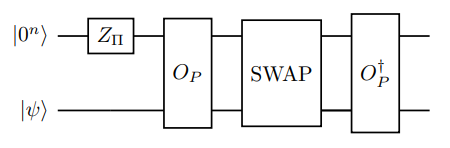
\includegraphics[width=0.5\linewidth]{Images/implD.png}
%     \caption{Circuit for implementing one step of Szegedy's quantum walk operator}
%     \label{fig:implszqw}
% \end{figure}
% Let the decomposition of $D$ denoted by
% \[
% D\ket{v_i}=\lambda_i\ket{v_i}
% \]
% For each $\ket{v_i}$, the associated basis in the 2-dimensional subspace is $\mathcal{B}_i=\{\ket{0^m}\ket{v_i},\ket{\perp_i}\}$. Then the qubitization procedure gives
% \[
% [O_Z]_{\mathcal{B}_i}=\begin{pmatrix} \lambda_i & -\sqrt{1-\lambda_i^2}\\ \sqrt{1-\lambda_i^2} & \lambda_i \end{pmatrix}
% \]
% The eigenvalue of $O_Z$ in the $2\times 2$ matrix block are 
% \[
% e^{\pm \iota arccos(\lambda_i)}
% \]
% This relation is important for the following reason. By proposition, if a Markov chain is reversible and ergodic, the eigenvalue of $D$ and $P$ are the same. In particular, the largest eigenvalue of $D$ is unique and is equal to $1$, and the second largest eigenvalue of $D$ is $1-\delta$, where $\delta>0$ is called the spectral gap. Since $arccos(1)=0$, and $arccos(1-\delta)\approx\sqrt{2\delta}$, we find that the spectral gap of $O_Z$ on the unit circle is in fact $\mathcal{O}(\sqrt{\delta})$ instead of $\mathcal{O}(\delta)$. This is called the spectral gap amplification, which leads to e.g. the quadratic quantum speedup of the hitting time.

% \begin{example}
%     (Determining whether there is a marked vertex in a complete graph). Let $G=(V,E)$ be a complete, graph of $N=2^n$ vertices. We would like to distinguish the following tww scenarios:
%     \begin{enumerate}
%         \item All vertices are the same, and the random wal is given by the transition matrix
%         \[
%         P=\frac{1}{N}ee^T, \quad e=(1,\ldots,1)^T
%         \]
%         \item There is one marked vertex. Without loss of generality we may assume this is the 0-th vertex (of course we do not have access to this information). In this case, the transition matrix is
%         \[
%         \tilde{P}_{ij}=\begin{cases}\delta_{ij}, &i=0\\P_{ij}, &i>0 \end{cases}
%         \]
%     \end{enumerate}
%     In other words, in case (2), the random walk will stop at the marked index. The transition matrix can also be writing in the block partitioned form as
%         \[
%         \tilde{P}=\begin{pmatrix} 1 & 0 \\ \frac{1}{N}\tilde{e} & \frac{1}{N}\tilde{e}\tilde{e}^T \end{pmatrix}
%         \]
%         Here $\tilde{e}$ is an all 1 vector of length $N-1$.
% \end{example}

% For the random walk defined by $P$, the stationary state is $\pi=\frac{1}{N}e$, and the spectral gap is $1$. For the random walk defined by $\tilde{P}$, the stationary state is $\tilde{\pi}=(1,0,\ldots,0)^T$ and the spectral gap of $\delta=N^{-1}$. Starting from the uniform state $\pi$, the probability distribution after $k$ steps of random walk is $\pi^T\tilde{P}^k$. Starting from the uniform state $\pi$, the probability distribution after $k$ steps of random walk is $\pi^T\tilde{P}^k$. This converges to the stationary state of $\tilde{P}$, and hence reach the marked vertex after $\mathcal{O}(N)$ steps of walks.

% These properties are also inherited by the discriminant matrices, with $D=P$ and
% \[
% \tilde{D} = \begin{pmatrix} 1 & 0 \\ 0 & \frac{1}{N}\tilde{e}\tilde{e}^T \end{pmatrix}
% \]
% To distinguish the two cases, we are given a Szegedy quantum walk operator called $O$, which can be either $O_Z$ or $\tilde{O}_Z$, which is associated with $D$, $\tilde{D}$, respectively. The initial state is
% \[
% \ket{\psi_0}=\ket{0^n}(H^{\otimes n}\ket{0^n})
% \]
% Our strategy is to measure the expectation
% \[
% m_k=\bra{\psi_0}O^k\ket{\psi_0}
% \]
% which can be obtained via Hadamard's test.

% Before determining the value of $k$, first notice that if $O=O_Z$, then $O_Z\ket{\psi_0}=\ket{\psi_0}$. Hence $m_k=1$ for all values of $k$.

% On the other hand, if $O=\tilde{O}_Z$, we use the fact that $\tilde{D}$ only has two nonzero eigenvalues $1$ and $(N-1)/N=1-\delta$, with associated eigenvectors denoted by $\ket{\tilde{\pi}}$ and $\ket{\tilde{v}}=\frac{1}{\sqrt{N-1}}(0,1,1,\ldots,1)^T$, respectively. Furthermore,
% \[
% \ket{\psi_0}=\frac{1}{\sqrt{N}}\ket{0^n}T_k(1)\ket{\tilde{\pi}}+\sqrt{\frac{N-1}{N}}\ket{0^n}T_k(1-\delta)\ket{\tilde{v}}+\ket{\perp},
% \]
% where $\ket{\perp}$ is an unnormalized state satisfying $(\ket{0^n}\bra{0^n}\otimes I_n \ket{\perp}=0$. Then using $T_k(1)=1$ for all $k$, we have
% \[
% m_k=\frac{1}{N}+\left(1-\frac{1}{N}\right)T_k(1-\delta)
% \]
% Use the fact that $T_k(1-\delta)=\cos (karccos (1-\delta))$, in order to have $T_k(1-\delta)\approx 0$, the smallest $k$ satisfies
% \[
% k\approx \frac{\pi}{2arccos(1-\delta)}\approx \frac{\pi}{2\sqrt{2\delta}}=\frac{\pi\sqrt{N}}{2\sqrt{2}}
% \]
% There fore taking $k=\lceil \frac{\pi\sqrt{N}}{2\sqrt{2}}\rceil$, we have $m_k\approx 1/N$. Running Hadamard's test to constant accuracy allows us to distinguish the two scenarios.

% \begin{remark}
%     (Without using the hadamard test). Alternatively, we may evaluate the success probability of obtaining $0^n$ in the ancilla qubits, i.e.,
%     \[
%     p(0^n) =\|(\ket{0^n}\bra{0^n}\otimes I_n)O^k\ket{\psi_0}\|^2
%     \]
%     When $O=O_Z$, we have $p(0^n)=1$ with certainty. When $O=\tilde{O}_Z$,
%     \[
%     p(0^n)=\frac{1}{N}+\left(1-\frac{1}{N}\right)T_k^2 (1-\delta)
%     \]
%     So running the problem with $k=\lceil \frac{\pi\sqrt{N}}{2\sqrt{2}}\rceil$, we can distinguish between the two cases.
% \end{remark}
% \begin{remark}
%     (Comparison with Grover's search). It is natural to draw comparisons between Szegedy's quantum walk and Grover's search. The two algorithms make queries to different oracles, and both yield quadratic speedup compared to classical algorithms. The quantum walk is slightly weaker, since it only tells whether there is one marked vertex or not. On the other hand, Grover's search also finds the location of the marked vertex. Both algorithms consist of repeated usage of the product of two reflectors.. The number of iterations need to be carefully controlled. Indeed, choosing a polynomial degree four time as large would result in $m_k\approx 1$for the case with a marked vertex.
% \end{remark}

% \begin{remark}
%     (Comparison with QPE). Another possible solution of the problem of finding the marked vertex is to perform QPE on the Szegedy walk operator $O$ (which can be $O_Z$ or $\tilde{O}_Z$). The effectiveness of the method rests on the spectral gap amplification discussed above.
% \end{remark}

% \subsection{Comparison with the original version of Szegedy's quantum walk}
% The quantum walk procedure can also be presented as follows. using the $O_P$ oracle and the multi-qubit SWAP gate, we can define two set of quantum states
% \[
% \ket{\psi_j^1}=O_P\ket{0^n}\ket{j}=\sum_j \sqrt{P_{jk}}\ket{k}\ket{j}
% \]
% \[
% \ket{\psi_j^2}=SWAP(O_P\ket{0^n}\ket{j})=\sum_k \sqrt{P_{jk}}\ket{j}\ket{k}
% \]
% this defines two projection operators
% \[
% \prod_l =\sum_{j\in[N]} \ket{\psi_j^l}\bra{\psi_j^l}.\quad l=1,2,
% \]
% from which we can define two $2n$-qubit reflection operators $R_{\prod_l}=2\prod_l-I_{2n}$. Let us write down the reflection operators more explicitly. Using the resolution of identity,
% \[
% R_{\prod_l} O_P((2\ket{0^n}\bra{0^n}-I)\otimes I_n)O_P^{\dagger}=O_P(Z_{\prod}\otimes I_n)O_P^{\dagger}
% \]
% Similarly,
% \[
% R_{\prod_2}=SWAP O_p (Z_{\prod}\otimes I_n)O_P^{\dagger}SWAP
% \]
% The Szegedy's quantum walk operator takes the form
% \[
% U_Z=R_{\prod_2}R_{\prod_1}
% \]
% which is a rotation operator that resembles grover's algorithm. Note that
% \[
% U_Z=SWAP O_P (Z_{\prod}\otimes I_n)O_P^{\dagger}SWAP O_P(Z_{\prod}\otimes I_n)O_P^{\dagger}
% \]
% so
% \[
% O_P^{\dagger}U_Z(O_P^{\dagger})^{-1}=O_Z^2
% \]
% so the walk operator is the same as a block encoding of $T_2(D)$ using qubitization, up to a matrix similarity transformation, and the eigenvalues are the same. In particular, consider the matrix power $O_Z^k$, which provides a block encoding of the Chebyshev matrix polynomial $T_k(D)$. Then the difference between $O_Z^{2k}$ and $U_Z^k$ appears only at the beginning and end of the circuit.


% \section{Quantum walks}
% We will now modify the classical random walk algorithm to a quantum algorithm, where the distribution preserving matrix $P$ is changed to a norm preserving matrix $W(P)$ (i.e. Unitary)

% While the basis state of a classical random walk is the current vertex we are at, a basis state of a quantum walk has two registers, the first corresponding to the current vertex and the second corresponding to the previous vertex. Equivalently, a basis state of a quantum walk corresponds to an edge of the graph.

% Our resulting quantum walk algorithm for search will actually be quite analogous to Grover's algorithm. We will call a basis state $\ket{x}\ket{y}$ ``good" if $x$ is a marked vertex, and ``bad" otherwise. Define $\ket{p_x}=\sum_y \sqrt{P_{xy}}\ket{y}$ to be the uniform superposition over the neighbors of $x$. As for Grover, define ``good" and ``bad" states as the superpositions over good and bad basis states:
% \[
% \ket{G}=\frac{1}{\sqrt{|M|}}\sum_{x \in M}\ket{x}\ket{p_x} \quad \text{and}  \quad \ket{B}=\frac{1}{\sqrt{N-|M|}}\sum_{x \notin M}\ket{x}\ket{p_x}
% \]
% where $M$ denotes the set of marked vertices. Note that $\ket{G}$ is just uniform superposition over all edges $(x,y)$ where the first coordinate is marked, and $\ket{B}$ is just the uniform superposition over all edges $(x,y)$ where the first coordinate is not marked.

% If $\epsilon = |M|/N$ and $\theta=arcsin(\sqrt{\epsilon})$) then the uniform state over all edges can be written as
% \[
% \ket{U}=\frac{1}{\sqrt{N}}\sum_x \ket{x}\ket{p_x}= \sin(\theta)\ket{G}+\cos(\theta)\ket{B}
% \]
% Here is the algorithm for searching a marked vertex if an $\epsilon$-fraction is marked. As in grover, if we don't know then we just run the algorithm repeatedly with exponentially decreasing guesses for $\epsilon (1/2,1/4,1/8,\ldots)$. If at the end we still haven't found a marked item, we will conclude that probably none exists.
% \begin{enumerate}
%     \item Setup the starting state $\ket{U}$
%     \item Repeat the following $\mathcal{O}(1/\sqrt{\epsilon})$ times:
%     \begin{enumerate}[label=(\alph*)]
%         \item Reflect through $\ket{B}$
%         \item reflect through $\ket{U}$
%     \end{enumerate}
%     \item Measure the first register and check that the resulting vertex is marked.
% \end{enumerate}

% The description and analysis of the algorithm takes place in the 2-dimensional space spanned by $\ket{G}$ and $\ket{B}$. Assuming we know how to implement steps (a) and (b), the proof that this algorithm finds a marked vertex is the same as for Grover and for amplitude amplification. We start with $\ket{U}=\sin(\theta)\ket{G}+\cos(\theta)\ket{B}$. The two reflections (a) and (b) increase the angle from $\theta$ to $3\theta$, moving us towards the good state (similarly to the analysis for Grover, you can draw a 2-dimensional picture with axes $\ket{B}$ and $\ket{G}$ to see this). More generally, after $k$ applications of (a) and (b) our state has become
% \[
% \sin((2k+1)\theta)\ket{G}+\cos((2k+1)\theta)\ket{B}
% \]
% Choosing $k\approx \frac{\pi}{4\theta}=\mathcal{O}(1/\sqrt{\epsilon})$, we will have $\sin((2k+1)\theta)\approx 1$, at which point measuring the first register will probably yield a vertex $x$ that is marked. We now look more closely how to implement the two kinds of reflections.

% \begin{enumerate}[label=(\alph*)]
%     \item \textbf{Reflect through $\ket{B}$}. Reflecting through $\ket{B}$ is relatively straightforward: we just have to ``recognize" whether the first register contains a marked $x$, and put a $-1$ if so (note that this is really a reflection through the subspace spanned by the bad basis states, but restricted to the 2-dimensional subspace spanned by $\ket{G}$ and $\ket{B}$ that's the same as a reflection through $\ket{B}$).
%     \item \textbf{Reflect through $\ket{U}$} This is where the quantum walk comes in. Let $\mathcal{A}$ be the subspace span $\{\ket{x}\ket{p_x}\}$ and $\mathcal{B}$ be span $\{\ket{p_y}\ket{y}\}$. Let ref($\mathcal{A}$) and $ref(\mathcal{B}$) denote reflections through $\mathcal{A}$ and $\mathcal{B}$ respectively. Define $W(P)=ref(\mathcal{B})ref(\mathcal{A})$ to be the product of these two reflections. This is the unitary analogue of $P$. Suppose we are able to implement the following two operations (even in a controlled manner):
%     \begin{enumerate}
%         \item $\ket{x}\ket{0} \rightarrow \ket{x}\ket{p_x}$
%         \item $\ket{0}\ket{y} \rightarrow \ket{p_y}\ket{y}$
%     \end{enumerate}
%     Since (1)and (2) prepare a uniform superposition over the neighbors of $x$ and $y$, respectively, one can think of them as taking one classical walk step ``in superposition". Note that $ref(\mathcal{A})$ can be implemented by applying the inverse of (a), putting a minus if the second register is not $\ket{0}$, and applying (a). We can similarly implement $ref(\mathcal{B})$ using (2) and its inverse. Here we can think $W(P)=ref(\mathcal{B})ref(\mathcal{A})$ as corresponding to four steps of the classical walk in superposition.

%     To see how to implement the reflection through $\ket{U}$, let us consider the eigenvalues and eigenvectors of $W(P)$. The eigenvalue of $W(P)$ can be related to the eigenvalues of $\lambda_1,\lambda_2,\ldots$ of $P$ as follows.
%     Let $\theta_j \in [0,\pi/2]$ be such that $|\lambda_j|=\cos (\theta_j)$. We won't prove it here, but it turns out that the eigenvalues of $W(P)$ are of the form $e^{\pm 2\iota\theta_j}$ where $\theta_j \geq \sqrt{2\delta}$, because $1-\delta \geq |\lambda)j|=\cos(\theta_j)\geq 1 -\theta_j^2/2$. We want to implement a reflection $R(P)$ through the subspace spanned by the eigenvalue$-1$ eigenvectors of $W(P)$; restricted $R(P)$ through subspace spanned by $\ket{G}$ and $\ket{B}$ this will b the desired reflection through $\ket{U}$.
% \end{enumerate}


% \subsection{Continuous-time quantum walk}
% We will now introduce continuous-time quantum walk as a natural analog of continuous-time classical random walk, and we'll see some examples how the two kinds of processes differ.

% Random walks come in two flavors: discrete - and continuous-time random walk, so we consider this case first. Given a graph $G=(V,E)$, we define the continuous-time random walk on $G$ as follows. Let $A$ be the adjacency matrix of $G$, the $|V|\times |V|$ matrix with
% \[
% A_{j,k}=\begin{cases}1, &(j,k)\in E\\
% 0 &(j,k)\notin E\end{cases}
% \]
% for every pair $j,k\in V$. In particular, if we disallow self loops, then the diagonal of $A$ is zero. There is another matrix associated with $G$ that is nearly as important: the Laplacian of $G$, which has
% \[
% L_{j,k}=\begin{cases} -deg(j) &j=k\\
% 1 &(j,k)\in E\\
% 0 &\text{otherwise}\end{cases}
% \]
% where $deg(j)$ denotes the degree of vertex $j$. (The Laplacian is sometimes defined different than this -e.g. sometimes with the opposite sign. We use this definition because it makes $L$ as a discrete approximation of the Laplacian operator $\nabla^2$ in the continuum.)

% The continuous-time random walk on $G$ is defined as the solution of the differential equation
% \[
% \frac{d}{dt}p_j(t)=\sum_{k\in V}L_{jk}p_k(t)
% \]
% Here $p_j(t)$ denotes the probability associated with vertex $j$ at time $t$. This can be viewed as a discrete analogy of the diffusion equation. Note that
% \[
% \frac{d}{dt}\sum_{j\in V}p_j(t)=\sum_{j,k\in V}L_{jk}p_k(t)=0
% \]
% (since the columns of $L$ sum to $0$), which shows that an initially normalized distribution remains normalized: the evolution of the continuous-time random walk for any time $t$ is a stochastic process. The solution of the differential equation can be given in closed form as
% \[
% p(t)=e^{Lt}p(0)
% \]

% \chapter{Variational Algorithms}
% To write Variational algorithms: near-term hybrid quantum-classical algorithms that are ideal candidates to achieve quantum advantage. 
% The aim of this section is to learn:
% \begin{itemize}
%     \item each step in variational algorithm design workflow
%     \item trade offs associated with each step
%     \item how to use Qiskit Runtime primitives to optimize for speed and accuracy.
% \end{itemize}

% In this chapter we will see the specifics of variational algorithms and near-term hybrid quantum-classical algorithms based on the variational theorem of quantum mechanics. These algorithms can leverage the utility provided by today's non-fault-tolerant quantum computers, making them ideal candidates to achieve quantum advantage.

% \begin{figure}
%     \centering
%     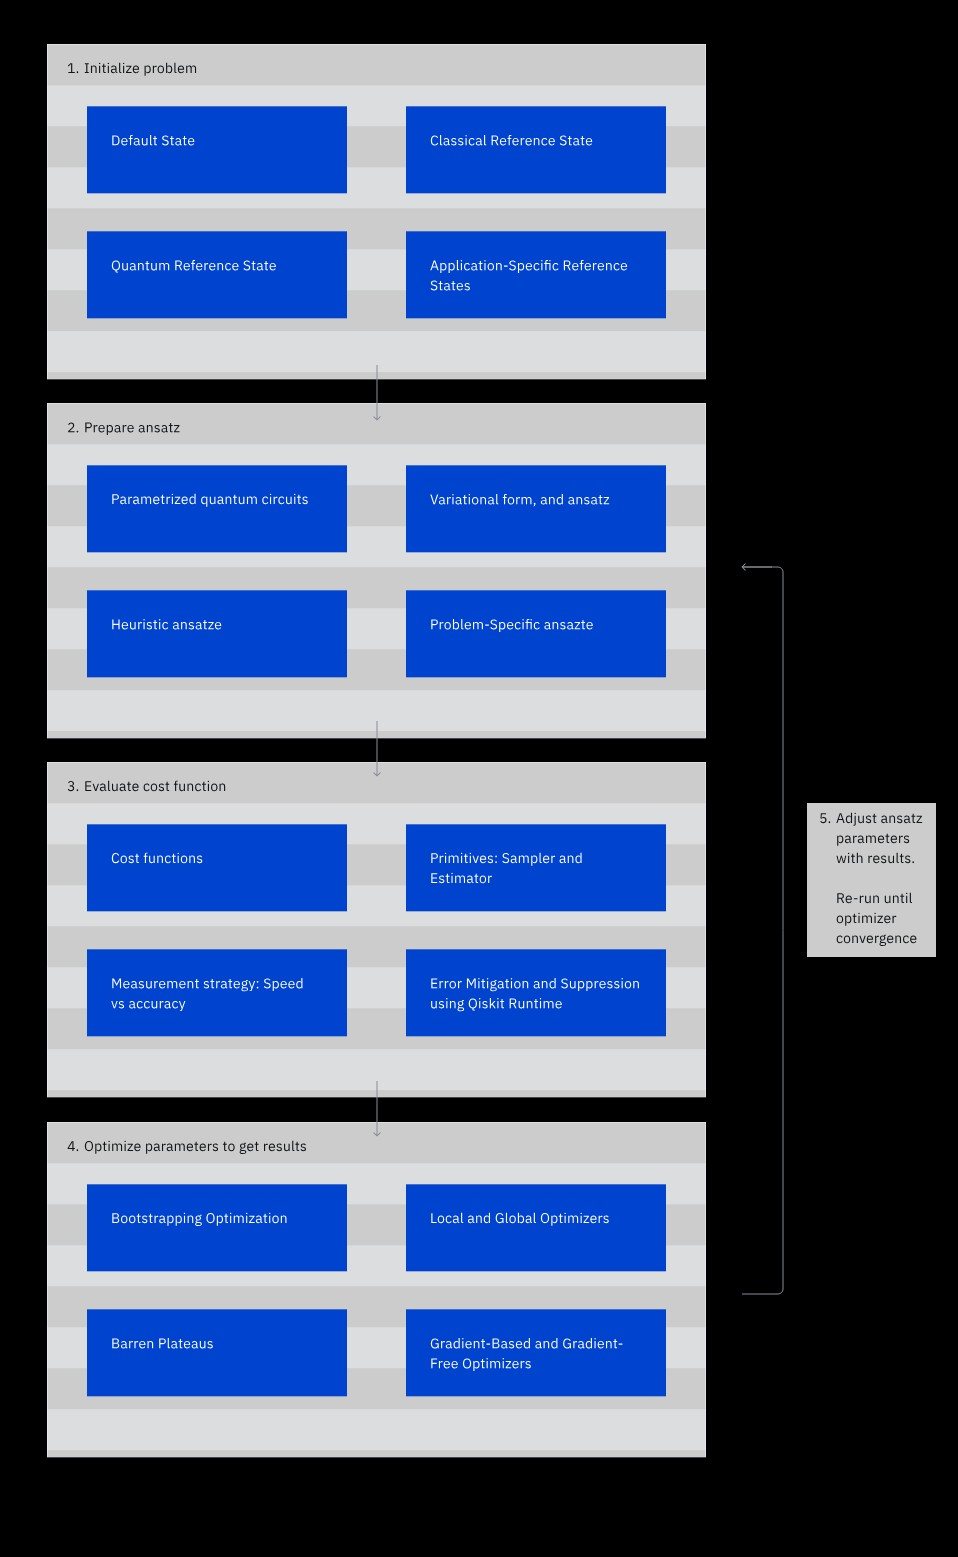
\includegraphics[width=0.75\linewidth]{Images/VQE_algo.png}
%     \caption{Variational Algorithm}
%     \label{figvqe_algo}
% \end{figure}

% Variational algorithms include several modular components that can be combined and optimized based on algorithm, software and hardware advancements. This includes a cost function that describes a specific problem with a set of parameters, an ansatz to express the search space with these parameters, and an optimizer to iteratively explore the search space. During each iterations, the optimizer evaluates the cost function with the current parameters and selects the next iteration's parameters until it converges on an optimal solution. The hybrid nature of this family of algorithms comes from the fact that the cost functions are evaluated using quantum resources and optimized through classical ones.

% \begin{enumerate}
%     \item \textbf{Initialize Problem: }Variational algorithms start by initializing the quantum computer in a default state $\ket{0}$, then transforming it to some desired (non-parameterized) state $\ket{\rho}$, which we will call \textit{reference state}.\\
%     This transformation is represented by the application of a unitary reference operator $U_R$ on the default state, such that $U_R\ket{0}=\ket{\rho}$.
%     \item \textbf{Prepare ansatz: }To begin iteratively optimizing from the default state $\ket{0}$ to the target state $\ket{\psi(\vec{\theta})}$, we must define a \textit{variational form} $U_V(\vec{\theta})$ to represent a collection of parameterized states for our variational algorithm to explore.\\
%     We refer to any particular combination of reference state and variational form as an ansatz state such that $U_A(\vec{\theta}):=U_V(\vec{\theta})U_R$. Ansatze will ultimately take the form of parameterize quantum circuits capable of taking the default state $\ket{0}$ to the target state $\ket{\psi(\vec{\theta})}$.\\
%     All in all we will have:
%     \begin{align*}
%         \ket{0}\xrightarrow{U_R} U_R\ket{0}&=\ket{\rho}\xrightarrow{U_V(\vec{\theta})} U_A(\vec{\theta})\ket{0}\\
%         &=U_V(\vec{\theta})U_R\ket{0}\\
%         &=U_V(\vec{\theta})\ket{\rho}\\
%         &=\ket{\psi(\vec{\theta})}
%     \end{align*}
%     \item \textbf{Evaluate Cost function: }We can encode our problem into a \textit{cost function} $C(\vec{\theta})$ as a linear combination of Pauli operators , run on a quantum system. While this can be information about a physical system, such as energy or spin, we can also encode non-physical problems as well. We can leverage Qiskit Runtime primitives to address noise with error suppression and mitigation while evaluating our cost function.
%     \item \textbf{Optimize Parameters: }Evaluations are taken to a classical computer, where a classical optimizer analyzes them and chooses the next set of values for the variational parameters. If we have a pre-existing optimal solution, we can set it as an \textit{initial point} $\vec{\theta_0}$ to bootstrap our optimization. Using this \textit{initial state} $\ket{\psi(\vec{\theta_0})}$ could help our optimizer find a valid solution faster.
%     \item \textbf{Adjust ansatz parameters with results, and re-run: }the entire process is repeated until the classical optimizer's finalization criteria are met, and an optimal set of parameter values $\vec{\theta^*}$ is returned. the proposed solution state for our problem will be $\ket{\psi(\vec{\theta}^*)}=U_A(\vec{\theta^*})\ket{0}$.
% \end{enumerate}

% \section{Variational Theorem}
% A common goal of variational algorithms is to find the quantum state with the lowest or highest eigenvalue of a certain observable. A key insight we'll use is the variation theorem of quantum mechanics. before going into its full statement, let us explore some of the mathematical intuition behind it.

% \subsection{Mathematical intuition for energy and ground state}
% In quantum mechanics, energy comes in the form of a quantum observable usually referred to as the \textit{Hamiltonian} (Hermitian matrix), which we'll denote by $\hat{\mathcal{H}}$. let us consider its spectral decomposition:
% \[
% \hat{\mathcal{H}}=\sum_{k=0}^{N-1} \lambda_k\ket{\phi_k}\bra{\phi_k}
% \]
% where $N$ is the dimensionality of the space of state, $\lambda_k$ is the k-th eigenvalue or, physically, the k-th energy level, and $\ket{\phi_k}$ is the corresponding eigen state: $\hat{\mathcal{H}}\ket{\phi_k}=\lambda_k\ket{\phi_k}$, the expected energy of a system in the (normalized) state $\ket{\psi}$ will be:
% \begin{align*}
% \braket{\psi|\hat{\mathcal{H}}|\psi}&=\braket{\psi|\left(\sum_{k=0}^{N-1}\lambda_k\ket{\phi_k}\bra{k}\right)|\psi}\\
% &=\sum_{k=0}^{N-1}\lambda_k\braket{\psi|\phi_k}\braket{\phi_k|\psi}\\
% &=\sum_{k=0}^{N-1}\lambda_k|\braket{\phi_k|\psi}|^2
% \end{align*}
% If we take into account that $\lambda_0\leq\lambda_k, \forall k$, we have:
% \begin{align*}
%     \braket{\psi|\hat{\mathcal{H}}|\psi}&=\sum_{k=0}^{N-1}\lambda_k|\braket{\phi_k|\psi}|^2\\
%     &\geq \sum_{k=0}^{N-1} \lambda_0|\braket{\phi_k|\psi}|^2\\
%     &=\lambda_0\sum_{k=0}^{N-1}|\braket{\phi_k|\psi}|^2\\
%     &=\lambda_0
% \end{align*}
% Since $\{\ket{\phi_k}\}_{k=0}^{N-1}$ is an orthonormal basis, the probability of measuring $\ket{\phi_k}$ is $p_k=|\braket{\psi|\phi_k}|^2$, and the sum of all the probabilities is such that $\sum_{k=0}^{N-1}|\braket{\psi|\phi_k}|^2=\sum_{k=0}^{N-1}p_k=1$. In short, the expected energy of any system is higher than the lowest energy or ground state energy:
% \[
% \braket{\psi|\hat{\mathcal{H}}|\psi}\geq \lambda_0
% \]
% the above argument applies to any valid (normalized) quantum state $\ket{\psi}$, so it is perfectly possible to consider parameterized state $\ket{\psi(\vec{\theta})}$ that depends on a parameter vector $\vec{\theta}$. This is where the "variational" part comes into play. If we consider a cost function given by $C(\vec{\theta}):=\braket{\psi(\vec{\theta})|\hat{\mathcal{H}}|\psi(\vec{\theta})}$ and we want to minimize it, the minimum will always satisfy:
% \[
% \min_{\vec{\theta}}C(\vec{\theta}) = \min_{\vec{\theta}} \braket{\psi(\vec{\theta}|\hat{\mathcal{H}}|\psi(\vec{\theta})}\geq \lambda_0
% \]
% The minimum value of $C(\vec{\theta})$ will be the closest that one can get to $\lambda_0$ using the parameterized state $\ket{\psi(\vec{\theta})}$, and equality will only be reached it there exists a parameter vector $\vec{\theta^*}$ such that $\ket{\psi(\vec{\theta^*})}=\ket{\phi_0}$

% \subsection{Variational theorem of Quantum Mechanics}
% If the (normalized) state $\ket{\psi}$ of a quantum system depends on a parameter vector $\vec{\theta}$, then the optimal approximation of the ground state (i.e. the eigen state $\ket{\phi_0}$ with the minimum value $\lambda_0$) is the one that minimizes the expectation value of the Hamiltonian $\hat{\mathcal{H}}$:
% \[
% \braket{\hat{\mathcal{H}}}(\vec{\theta}):=\braket{\psi(\vec{\theta})|\hat{\mathcal{H}}|\psi(\vec{\theta})} \geq \lambda_0
% \]
% The reason why the variational theorem is stated in terms of energy minima is that it includes a number of mathematical assumptions:
% \begin{itemize}
%     \item For physical reasons, a finite lower bound to the energy $E\geq \lambda_0>-\infty$ needs to exist, even for $N\rightarrow \infty$.
%     \item Upper bounds do not generally exist.
% \end{itemize}
% However, mathematically speaking, there is nothing special about the Hamiltonian $\hat{\mathcal{H}}$ beyond these assumptions, so the theorem can be generalized to other quantum observables and their eigenstates provided they follow the same constraints. Also, note that if finite upperbounds exist, the same mathematical arguments could be made for maximizing eigen values by swapping lower bounds for upper bounds.

% \section{Reference States}
% In this section, we will explore how we can initialize our system with a reference state to help our variational algorithm converge faster. First, we will learn how to construct a reference state manually, and then explore several standard options that can be used in a variational algorithm.

% \subsection{Default State}
% A \textit{reference state} refers to the initial fixed part of our problem. To prepare a reference state, we need to apply the appropriate, non -parameterized unitary $U_R$ at the start of out quantum circuit, such that $\ket{\rho}=U_R\ket{0}$. If you have an educated guess or data point from an existing optimal solution, the variational algorithm will likely converge faster if you use that as a starting point.

% The simplest possible reference state is the default state, where we use the starting state of an n-qubit quantum circuit: $\ket{0^{\otimes n}}$. For the default state, our unitary operator $U_R=I$. Due to its simplicity, the default state is a valid reference state used in many scenarios.

% \subsection{Classical Reference state}
% Suppose you have a 3-qubit system and you want to start in the state $\ket{001}$ instead of the default state $\ket{000}$. This is an example of a purely classical reference state, and to construct it, you simply need to apply an X gate to qubit 0 (following Qiskit's qubit ordering), as $\ket{001}=X_0\ket{000}$.
% \begin{figure}[ht]
%     \centering
%     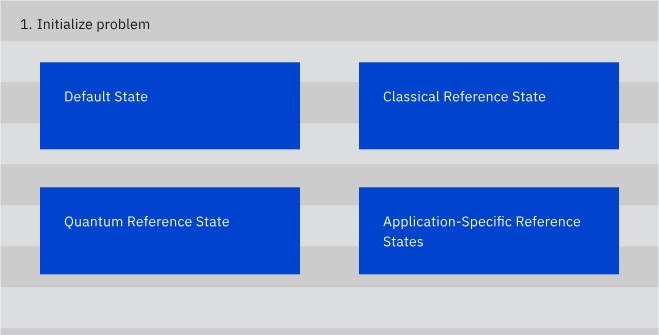
\includegraphics[width=0.25\linewidth]{Images/ref_state.png}
%     \caption{Reference state}
%     \label{fig:ref_state}
% \end{figure}
% In this case, our unitary operator $U_R=X_0$, which leads to the reference state $\ket{\rho}=\ket{001}$.
% \begin{lstlisting}[language=Python]
% from qiskit import QuantumCircuit
% qc=QuantumCircuit(3)
% qc.x(0)

% qc.draw("mpl")
% \end{lstlisting}
% This outputs the following circuit:
% \begin{figure}[ht]
%     \centering
%     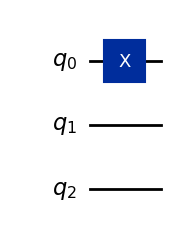
\includegraphics[width=0.25\linewidth]{Images/ref_state_dia.png}
%     \caption{Classical Reference State Circuit}
%     \label{fig:ref_state_classical}
% \end{figure}
% \subsection{Quantum Reference State}
% Suppose you aim to start with a more complex state that involves superposition and/or entanglement such as $\frac{1}{\sqrt{2}}(\ket{100}+\ket{111})$.

% To obtain this state from $\ket{000}$, one approach is to use a hadamard gate on qubit $0 (H_0)$, a CNOT(CX) gate with qubit 0 as the control qubit and qubit 1 as the target qubit ($CNOT_{01}$), and finally an X gate applied to qubit 2 ($X_2$).

% In this scenario, our unitary operator is $U_R=X_2CNOT_{01}H_0\ket{000}$, and our reference state is $\ket{\rho}=\frac{1}{\sqrt{2}}(\ket{100}+\ket{111}$.
% \begin{lstlisting}[language=Python]
% qc=QuantumCircuit(3)
% qc.h(0)
% qc.cx(0,1)
% qc.x(2)

% qc.draw(``mpl")
% \end{lstlisting}
% This outputs the following circuit \ref{fig:ref_state_quantum}:
% \begin{figure}[ht]
%     \centering
%     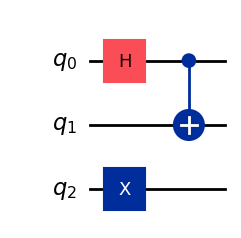
\includegraphics[width=0.25\linewidth]{Images/ref_state_quantum.png}
%     \caption{Quantum Reference State}
%     \label{fig:ref_state_quantum}
% \end{figure}

% \subsection{Constructing Reference States using template circuits}
% We can also use various template circuits, such as Twolocal which allows for expressing multiple tunable parameters and entanglements with ease. We will cover these template circuits in more detail in the next section, but we can use them fr our reference state if we bind the parameters.
% \begin{lstlisting}[language=Python]
% from qiskit.circuit.library import TwoLocal
% from math import pi

% reference_circuit = twoLocal(2,"rx","cz",entanglement="linear",reps=1)
% theta_list = [pi//2,pi/2,pi/2,pi/2]

% reference_circuit = reference_circuit.assign_parameters(theta_list)

% reference_circuit.decompose().draw("mpl")
% \end{lstlisting}
% This outputs the following circuit:
% \begin{figure}[ht]
%     \centering
%     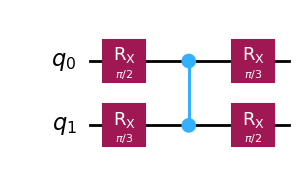
\includegraphics[width=0.5\linewidth]{Images/ref_state_template.png}
%     \caption{Reference State using Template}
%     \label{fig:ref_state_template}
% \end{figure}

% \subsection{Application Specific Reference States}
% \subsubsection{Quantum Machine Learning}
% In the context of a variational quantum classifier (VQC), the training data is encoded into a quantum state with a parameterized circuit known as a feature map, where each parameter value represents a data point from the training dataset. The ZZFeatureMap is a type of parameterized circuit that can be utilized to pass our data point(x) to this feature map.

% \begin{lstlisting}[language=Python]
% from qiskit.circuit.library import ZZFeatureMap
% data=[0.1,0.2]

% zz_feature_map_reference = ZZFeatureMap(feature_dimension=2, reps=2)
% zz_feature_map_reference = zz_feature_map_reference.assign_parameters(data)
% zz_feature_map_reference.decompose().draw("mpl")
% \end{lstlisting}
% This outputs the following circuit:
% \begin{figure}[ht]
%     \centering
%     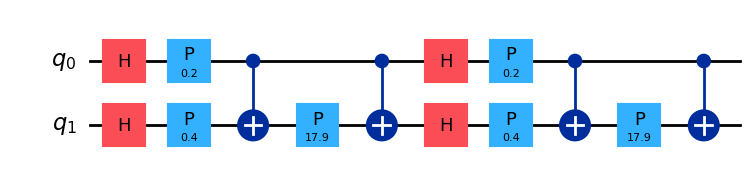
\includegraphics[width=0.5\linewidth]{Images/ref_state_zzfmap.png}
%     \caption{Reference State using ZZFeatureMap}
%     \label{fig:ref_state_zzfmap}
% \end{figure}

% \section{Ansatze and Variational Forms}
% At the heart of all variational algorithm  lies the key idea of analyzing the differences between states, which are conveniently related through some well-behaved mapping (e.g., continuous, differentiable) from a set of parameters or variables - hence the name.

% First, we'll explore how to construct parameterized circuits by hand. We'll use these circuits to define a variational form that represents a collection of parameterized states for our variational algorithms to explore. Then, we'll construct our ansatz by applying this variational form to our reference state.

% We'll also explore how to trade off speed versus accuracy while exploring this search space.
% \begin{figure}
%     \centering
%     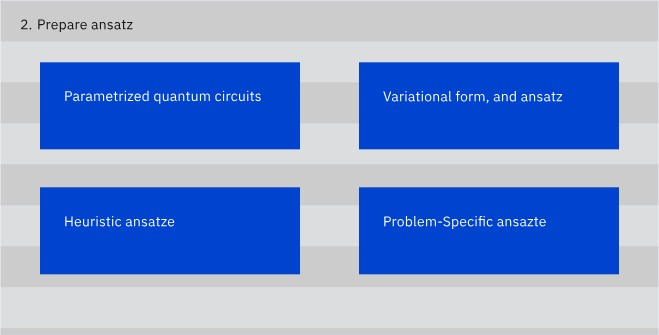
\includegraphics[width=0.5\linewidth]{Images/prep_ansatz.png}
%     \caption{Prepare Ansatz}
%     \label{fig:prep_ansatz}
% \end{figure}
% \subsection{Parameterized Quantum Circuits}
% Variational algorithms operate by exploring and comparing a range of quantum state $\ket{\psi(\vec{\theta})}$, which depends on a finite set of k parameters $\vec{\theta}=(\theta^0,\ldots,\theta^{k-1})$. These states can be prepared using a parameterized quantum circuit, where gates are defined with tunable parameters. It is possible to create this parameterized circuit without binding specific angles yet:
% \begin{lstlisting}[language=Python]
% from qiskit.circuit import QuantumCircuit, Parameter

% theta = Parameter("theta")

% qc = QuantumCircuit(3)
% qc.rx(theta, 0)
% qc.cx(0, 1)
% qc.x(2)

% qc.draw("mpl")
% \end{lstlisting}
% This outputs the following parameterized circuit:
% \begin{figure}[ht]
%     \centering
%     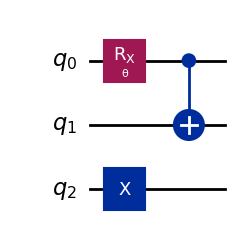
\includegraphics[width=0.25\linewidth]{Images/param_qc.png}
%     \caption{Parameterized Quantum Circuit}
%     \label{fig:param_qc}
% \end{figure}
% \begin{lstlisting}[language=Python]
% from math import pi

% angle_list=[pi/3, pi/2]
% circuits = [qc.assign_parameters({theta:angle} from angle in angle_list)]

% for circuit in circuits:
%     display(cicuit.draw("mpl")
% \end{lstlisting}
% This outputs the following circuits:
% \begin{figure}[ht]
%     \centering
%     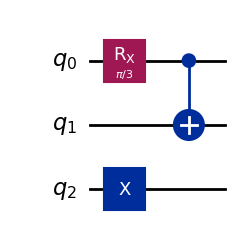
\includegraphics[width=0.25\linewidth]{Images/param_ex1.png}
%     \caption{For $\theta=\pi / 3$}
%     \label{fig:param_ex1}
% \end{figure}
% \begin{figure}[ht]
%     \centering
%     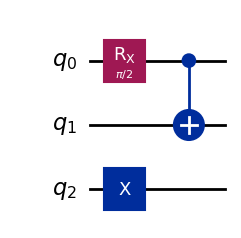
\includegraphics[width=0.25\linewidth]{Images/param_ex2.png}
%     \caption{For $\theta = \pi/2 $}
%     \label{fig:param_ex2}
% \end{figure}
% \subsection{Variational Form and Ansatz}
% To iteratively optimize from a reference state $\ket{\rho}$ to a target state $\ket{\psi(\vec{\theta})}$, we need to define a variational form $U_V(\vec{\theta})$ that represents a collection of parameterized state for our variational algorithm to explore:
% \begin{align*}
%     \ket{0}\xrightarrow{U_R} U_R\ket{0}&=\ket{\rho}\xrightarrow{U_V(\vec{\theta}}U_A(\vec{\theta}\ket{0}\\
%     &=U_V(\vec{\theta})U_R\ket{0}\\
%     &=U_V(\vec{\theta})\ket{\rho}\\
%     &=\ket{\psi(\vec{\theta})}
% \end{align*}
% Note that the parameterized state depends on both the reference state $\ket{\rho}$, which does not depends on any parameters, and the variational form $U_V(\vec{\theta})$, which always depends on parameters. We refer to the combination of these two halves as an ansatz: $U_A(\vec{\theta}):=U_V(\vec{\theta})U_R$.

% Now, we have to construct an ansatz which represents a collection of parameterized states based on the different values of parameter vectors $\vec{\theta}$ we wish to explore thus, creating a collection of parameterized quantum states $\ket{\psi(\vec{\theta})}$ to find the minima of the cost function $C(\vec{\theta})=\bra{\psi(\vec{\theta})}|H|\ket{\psi(\vec{\theta})}$.
% As we construct our ansatz to represent a collection of parameterized states for our variational algorithm to explore, we realize an important issue: dimensionality. An n-qubit system (i.e., Hilbert space) ha a vast number of distinct quantum states in the configuration space. We would require an unwieldy number of parameters to fully explore it. Quantitatively, its dimensionality is $D=2^{2n}$ because of the $2^n$-complex entries of the $n$-dimensional Hilbert space requiring two real numbers each. To make matters worse, the runtime complexity of search algorithms, and others alike, grows exponentially with this dimensionality, a phenomenon often referred to in the literature as the curse of dimensionality.

% To counter this setback, it is common practice to impose some reasonable constraints on the variational form such that only the most relevant states are explored. Finding an efficient truncated ansatz is an active area of research, but we'll cover two common designs.
% \subsubsection{Heuristic ansatze and trade-offs}
% If you do not have any information about your particular problem that can help restrict the dimensionality, you can try any arbitrary family of parameterized circuits with fewer than $2^{2n}$. However, there are some trade-offs to consider:
% \begin{itemize}
%     \item \textbf{Speed: } By reducing the search space, the algorithm can run faster.
%     \item \textbf{Accuracy: } However, reducing the space could risk excluding the actual solution to the problem, leading to suboptimal solutions.
%     \item Noise: Deeper circuits are affected by noise, so we need to experiment with out ansatz's connectivity, gates and gate fidelity.
% \end{itemize}
% There is a fundamental trade-off between quality (or even solvability) and speed: the more parameters, the more likely you are to find a precise result, but the longer it will take to run the algorithm.

% \subsubsection{N-local circuits}
% One of the most widely used examples of heurisitc ansatzes is the N-loca circuits, for a few reasons:
% \begin{itemize}
%     \item \textbf{Efficient Implementation: } The N-local ansatz is typically composed of simple, local gates that can be implemented efficiently on a quantum computer, using a small number of physical qubits. This makes it easier to construct and optimize quantum circuits.
%     \item \textbf{Captures important correlations: } The N-local ansatz can capture important correlations between the qubits in a quantum system, even with a small number of gates. This is because the local gates can act on neighboring qubits and create entanglement between them, which can be important for simulation complex quantum systems.
% \end{itemize}
% These circuits consist of rotation and entanglement layers that are repeated alternatively one or more times as follows:
% \begin{itemize}
%     \item Each layer if formed by gates of size at most N, where N has to be lower than the number of qubits.
%     \item For a rotation layer, the gates are stacked on top of each other. We can use standard rotation operations such as RX or CRZ. For an entanglement layer, we can use gates like Toffoli gates or CS with an entanglement strategy.
%     \item Both types of layers can be parameterized or not, but at least one of them needs to contain parameters. Otherwise, without at least one parameter, there wouldn't be any variations!
%     \item Optionally, an extra rotation layer can be added to the end of the circuit.
% \end{itemize}
% For example, let's create a 5-qubit Nlocal circuit with rotation blocks formed by RX and CRZ gates, entanglement blocks formed by Toffoli gates that at on n qubits $[0,1,2], [0,2,3],[4,2,1]$ and $[3,1,0]$ and 2 repitions of each layer.
% \begin{lstlisting}[language=Python]
% from qiskit.circuit.library import NLocal, CCXGate, CRZgate, RXGate
% from qiskit.circuit import Parameter

% theta=Parameter("theta")
% ansatz=NLocal(num_qubits=5,rotation_blocks=[RXGate(theta), CRZGate9theta)],entanglement_blocks=CCXGate(),entanglement=[[0,1,2],[0,2,3],[4,2,1],[3,1,0]],reps=2,insert_barriers=True)
% ansatz.decompose().draw("mpl")
% \end{lstlisting}
% This results in the following circuit:

% \begin{figure}[ht]
%     \centering
%     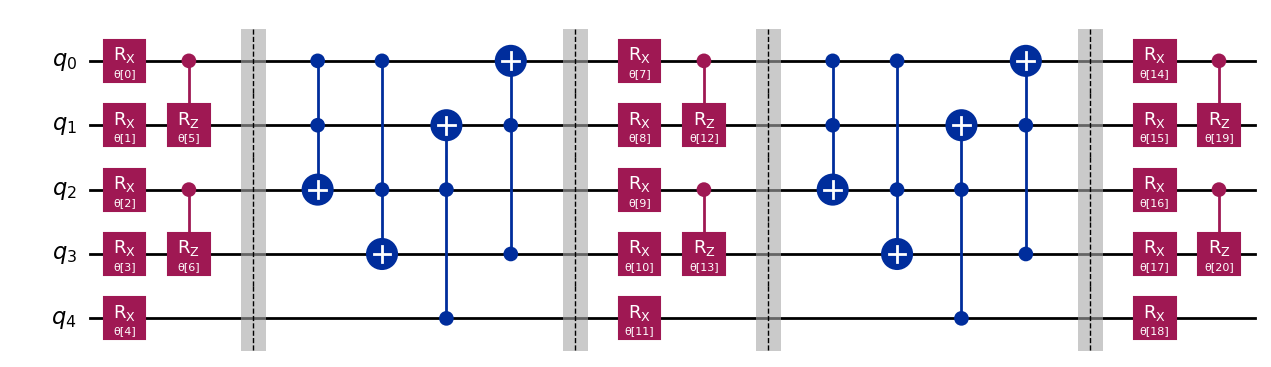
\includegraphics[width=0.5\linewidth]{Images/5q_ansatz_ex.png}
%     \caption{NLocal 5qubit example Circuit}
%     \label{fig:5q_ansatz_ex}
% \end{figure}

% In the above example, the largest gate is the Toffoli gate, which acts on three qubits, making the circuit 3-local. The most commonly used type of N-local circuits are 2-local circuits with single-qubit rotation gates and 2-qubit entanglement gates.

% Let's create a 2-local circuit using Qiskit's TwoLocal class. The syntax is the same as NLocal, but there are some differences. For instance, most gates, such as RX, RZ, and CNOT, can be passed as strings without importing the gates or creating a Parameter instance.

% \begin{lstlisting}[language=Python]
% from qiskit.circuit.library import TwoLocal

% ansatz=TwoLocal(numqubits=5, rotation_blocks=["rx","rz"]], entanglement_blocks="cx",entanglement="linear",reps=2,insert_barriers=True,)
% ansatz.decompose().draw("mpl")
% \end{lstlisting}
% The circuit will be as shown:
% \begin{figure}[ht]
%     \centering
%     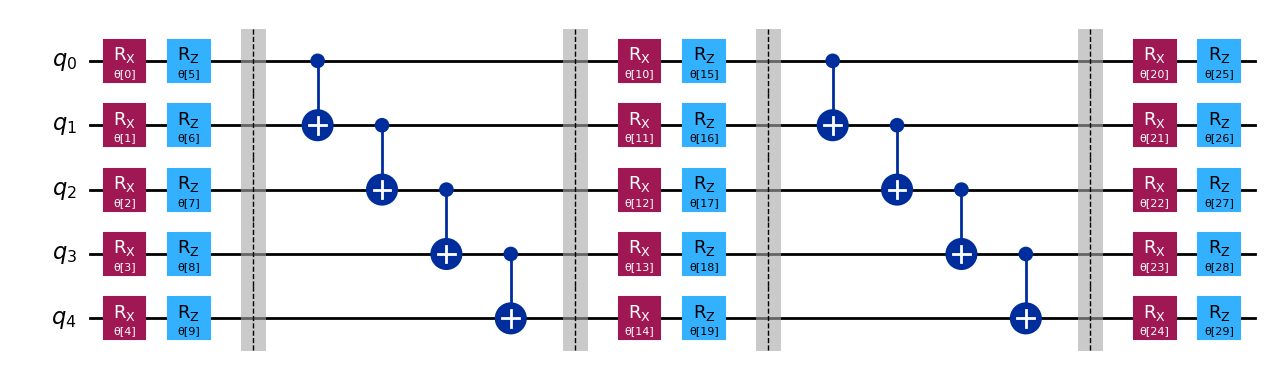
\includegraphics[width=0.5\linewidth]{Images/2local_ansatz.png}
%     \caption{TwoLocal Ansatz Circuit Example}
%     \label{fig:2local_ansatz}
% \end{figure}
% In this case, we used the linear entanglement distribution, where each qubit is entangled with the next. to learn about other strategies, refer to Twolocal's documentation.

% \subsubsection{EfficientSU2}
% EfficientSU2 is a hardware-efficient circuit that consists of single-qubit operations spanning SU(2) and CX entanglements. This is a heuristic pattern that can be used to prepare trial wave functions for variational quantum algorithms or as a classification circuit for machine learning.
% \begin{lstlisting}[language=Python]
% from qiskit.circuit.library import EfficientSU2

% ansatz=EfficientSU2(4,su2-gates=["rx',"y"],entanglement="linear",reps=1)
% ansatz.decompose().draw("mpl")
% \end{lstlisting}
% This results in following circuit:
% \begin{figure}[ht]
%     \centering
%     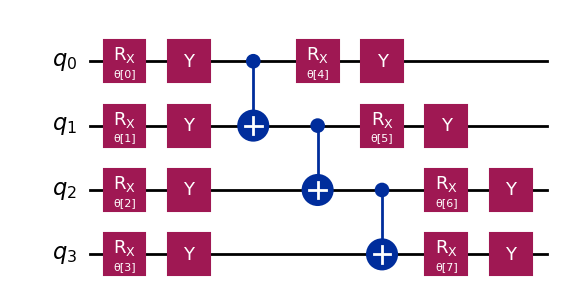
\includegraphics[width=0.5\linewidth]{Images/efficientsu2_ansatz.png}
%     \caption{EfficientSU2 ansatze}
%     \label{fig:efficeintsu2}
% \end{figure}
% \subsection{Problem-specific ansatze}
% While heuristic and hardware efficient ansatze help us to solve a problem in a naive way, we can cause problem-specific knowledge to restrict our circuit search space to a specific type. This will help us to gain speed without losing accuracy in our search process.

% \subsubsection{Optimization}
% In a max-cut problem, we want to partition nodes of a graph in a way that maximizes the number of edges between nodes in different groups. The desired max-cut partition for the graph below is clear: the 0th node on the left should be separated from the rest of the nodes in the right by a cut.

% \begin{lstlisting}[language=Python]
% imoprt rustworkx as rx
% from rustworkx.visualization import mpl_draw

% n=4
% G=rx.PyGraph()
% G.add_nodes_from(range(n))
% # The edge syntax is (start, end, weight)
% edges=[(0,1,1.0),(0,2,1.0),(0,3,1.0),(1,2,1.0),(2,3,1.0)]
% G.add_edges_from(edges)

% mpl_draw(G, pos=rx.shell_layout(G),with_labels=True, edge_labels=str, node_color="#1192E8")
% \end{lstlisting}
% The following is the resulting graph:
% \begin{figure}
%     \centering
%     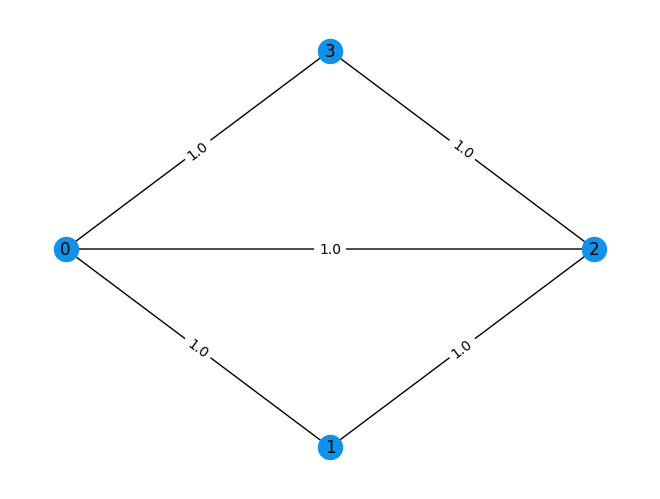
\includegraphics[width=0.5\linewidth]{Images/graph.png}
%     \caption{graph}
%     \label{fig:graph}
% \end{figure}

% To utilize QAOA algorithm from a max-cut problem, we require a Pauli-Hamiltonian that encodes the cost in a manner such that the minimum expectation value of the operator corresponds to the maximum number of edges between the nodes in two different groups.

% For this, simple example, the operator is a linear combination of terms with Z operators on nodes connected by an edge (recall that the 0th qubit is farthest right): ZZII+IZZI+ ZIIZ+IZIZ+IIZZ. Once the operator is constructed, the ansatz for the QAOA algorithm can easily be built by using the QAOA Ansatz circuit from the Qiskit circuit library.
% \begin{lstlisting}[language=Python]
% # Pre-defined ansatz circuit, operator class and visualization too:
% from qiskit.circuit.library import QAOAAnsatz
% from qiskit.quantum_info import SparsePauliOp

% # Problem to Hamiltonian operator
% hamiltonian = SparsePauliOp.from_list(["ZZII",1),("IZZI",1),("ZIIZ",1),("IZIZ",1),("IIZZ",1)]
% # QAOA ansatz circuit
% ansatz=QAOAAnsatz(hamiltonian, reps=2)
% # Draw
% ansatz.decompose(reps=3).draw("mpl")
% \end{lstlisting}
% \begin{figure}[ht]
%     \centering
%     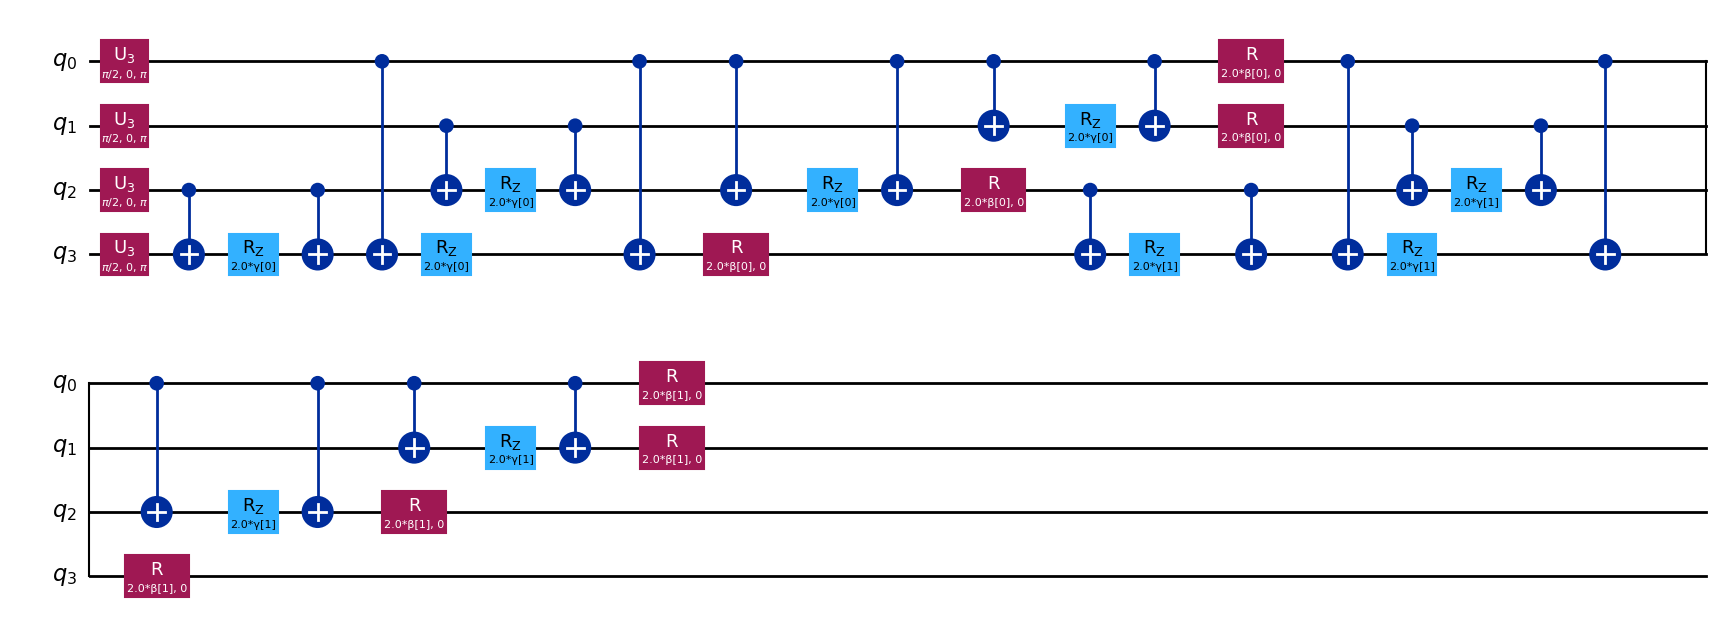
\includegraphics[width=0.5\linewidth]{Images/QAOA_circ.png}
%     \caption{QAOA circuit}
%     \label{fig:qaoa_circ}
% \end{figure}
% The previous image illsutrates the ansatz in basic gates for clarity. However, it can be expressed in multiple levels of decomposition by changing the reps argument or by drawing the circuit without the decompose method. for example, the following representation directly shows the QAOA structure with the default reps value, which is reps=1.
% \begin{lstlisting}[language=Python]
% ansatz.decompose(reps=1).draw("mpl")
% \end{lstlisting}
% \begin{figure}[ht]
%     \centering
%     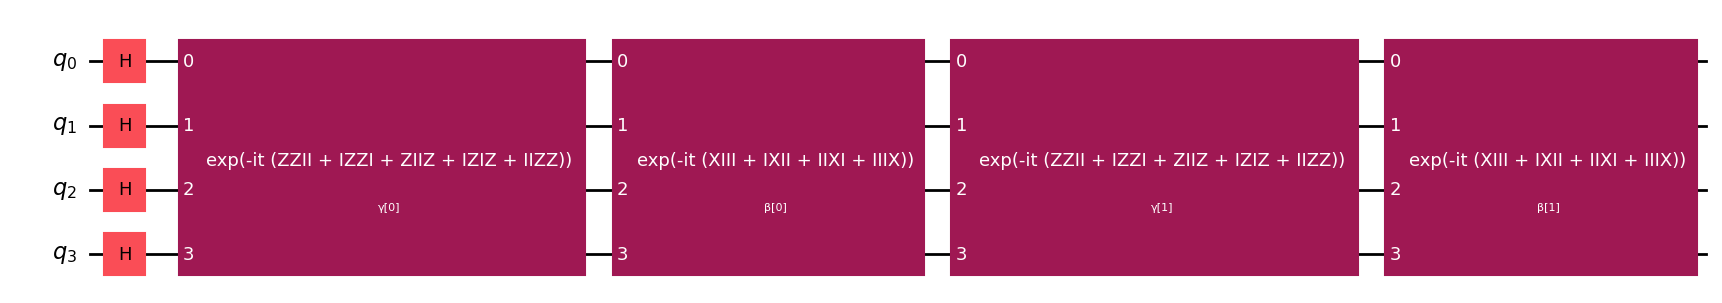
\includegraphics[width=0.5\linewidth]{Images/ansatz_reps1.png}
%     \caption{Decompose Circuit}
%     \label{fig:asnatz_reps1}
% \end{figure}

% \subsubsection{Quantum Machine Learing}
% In machine learning,  a common application is the classification of data into two or more categories. This involves encoding a datapoint into a feature map that maps classical feature vectors into the quantum hilbert space. Constructing quantum feature maps based on the parameterized quantum circuits. Constructing quantum feature meaps based on parameterized quantum circuits that are hard to simulate classically is an important step towards obtaining a potential adantage over classical machine learning approached and is an active are of current research.

% The ZZFeatureMap can be used to create a parameterized circuit. We can pass in our data points to the feature map $(x)$ and a separate variational form to pass in weights as parameters $(\theta)$
% \begin{lstlisting}
% from qiskit.circuit.library import ZZFeatureMap, TwoLocal

% data=[0.1,0.2]

% zz_feature_map_reference=ZZFeatureMap(feature_dimension=2,reps=2)
% zz_feature_map_reference= zz_feature_map_reference.assign_parameters(data)

% variation_form=TwoLocal(2,["ry","rz"],"cz",reps=2)
% vqc_ansatz = zz_feautre_map_reference.compose(vairation_form)
% vqc_ansatz.decompose().draw("mpl")
% \end{lstlisting}
% \begin{figure}[ht]
%     \centering
%     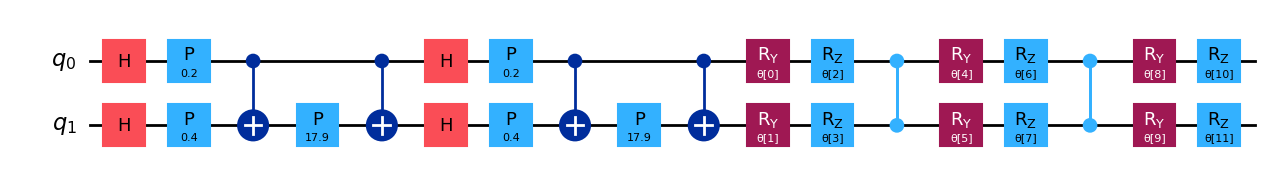
\includegraphics[width=0.5\linewidth]{Images/qml_circ.png}
%     \caption{ Circuit}
%     \label{fig:qlm_circ}
% \end{figure}

% The high-level variational workload looks as follows:
% \begin{figure}[ht]
%     \centering
%     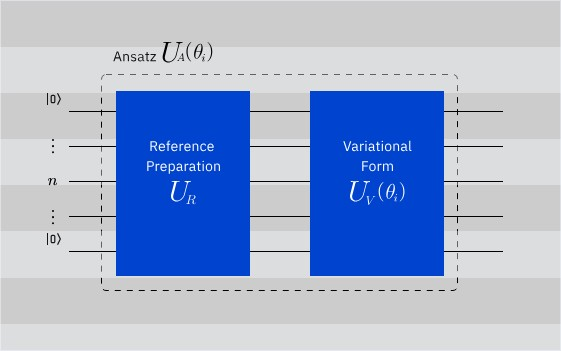
\includegraphics[width=0.5\linewidth]{Images/ansatz.png}
%     \caption{Variational workload}
%     \label{fig:ansatz}
% \end{figure}
% For each variation parameter $\vec{\theta}$, a different quantum state will be produced. to find the optimal parameters, we need to define a problem-specific cost function to iteratively update our ansatz's parameters.

% \section{Cost Functions}
% We now see how to evaluate a cost function:
% \begin{enumerate}
%     \item First, we will learn about Qiskit Runtime primitives
%     \item Define a cost function $C(\vec{\theta})$. This is a problem-specific function that defines the problems goal for the optimizer to minimize (or maximise)
%     \item Defining a measurement strategy with Qiskit Runtime primitves to optimize speed vs accuracy
% \end{enumerate}
% \begin{figure}[ht]
%     \centering
%     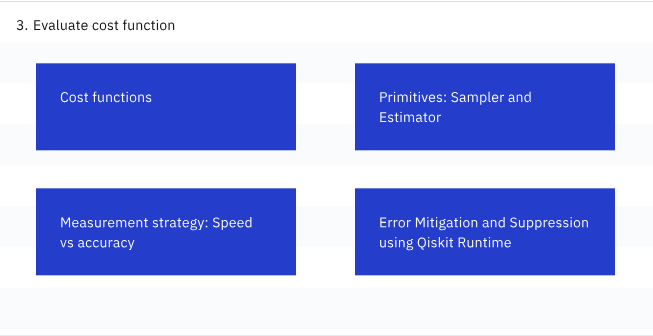
\includegraphics[width=0.75\linewidth]{Images/Costfunc.png}
%     \caption{Cost function}
%     \label{fig:cost_func}
% \end{figure}
% \subsection{Primitive}
% All physical systems, whether classical or quantum, exist in different states. For example, a car on a road can have a certain mass, position, speed, or accelerate that characterize its state. Similarly, quantum systems can also have different configurations or states, but they differ from classical system in how we deal with measurements and state evolution. This leads to unique properties such as superposition and entanglement that are exclusive to quantum mechanics. Just like we can describe a car's state using physical properties like speed or acceleration, we can also describe the state of a quantum system using observables, which are mathematical objects.

% In quantum mechanics, states are represented by normalized complex column vectors, or kets ($\ket{\psi})$, and \textbf{observable are hermitian operators} $\hat{H}=\hat{H}^{\dagger}$ that act on the kets. An eigenvector $(\ket{\lambda})$ of an observable is known as an eigenstate. Measuring an observable for one of its eigen states $(\ket{\lambda})$ will give us the corresponding eigenvalue $(\lambda)$ as readout.

% how to measure a quantum system and what can you measure, Qiskit offers two primitives that can help:
% \begin{itemize}
%     \item \textbf{Sampler: }Given a quantum state $\ket{\psi}$, this primitive obtains the probability of each possible computational basis state.
%     \item \textbf{Estimator: } Given a quantum observable $\hat{H}$ and a state $\ket{\psi}$, this primitive computes the expected value of $\hat{H}$.
% \end{itemize}

% \subsubsection{The Sampler Primitive}
% The $\textbf{Sampler}$ primitive calculates the probability of obtaining each possible state $\ket{k}$ from the computational basis, given a quantum circuit that prepare the state $\ket{\psi}$. It calculates
% \[
%     p_k=|\braket{k|\psi}|^2 \quad \forall k\in\mathbb{Z}_2^n \equiv \{0,1,\ldots, 2^n-1\}
% \]
% Qiskit Runtime's Sampler runs the circuit multiple times on a quantum device, performing measurements on each run, and reconstructing the probability distribution from the recovered bit strings. The more runs (or shots) it performs, the more accurate the results will be, but this requires more time and quantum resources.

% However, since the number of possible outputs grow exponentially with the number of qubits $n$ (i.e. $2^n$), the number of shots will need to grow exponentially as well in order to capture a dense probability distribution. Therefore, $\textbf{Sampler}$ is only efficient to sparse probability distributions; where the target state $\ket{\psi}$ must be expressible as a linear combination of the computational basis states, with the number of terms growing at most polynomially with the number of qubits:
% \[
% \ket{\psi} = \sum_k^{Poly(n)} w_k\ket{k}
% \]
% The \textbf{Sampler} can also be configured to retrieve probabilities from a subsection of the circuit representing a subset of the total possible states.

% \subsubsection{The Estimator Primitive}
% The \textbf{Estimator} primitive calculates the expectation value of an observable $\hat{H}$ for a quantum state $\ket{\psi}$; where the observable probabilities can be expressed as $p_{\lambda}=|\braket{\lambda|\psi}|^2$, being $\ket{\lambda}$ the eigen states of the observable $\hat{H}$. The expectation value is then defined as the average of all possible outcomes $\lambda$ (i.e. the eigenvalues of the observable) of a measurement of the state $\ket{\psi}$, weighted by the corresponding probabilities: 
% \[
% \braket{\psi|\hat{H}|\psi}=\braket{\hat{H}}_{\psi} :=\sum_{\lambda} \lambda\braket{\psi|\lambda}\braket{\lambda|\psi}=\sum_{\lambda} \lambda|\braket{\lambda|\psi}|^2=\sum_{\lambda} p_{\lambda} \lambda
% \]
% However, calculating the expectation value of an observable is not always possible, as we often don't know its eigenbasis. Qiskit Runtime's \textbf{Estimator} uses a complex algebraic process to estimate the expectation value on a real quantum device by breaking down the observable into a combination of other observables whose eigenbasis we do know.

% In simpler terms, \textbf{Estimator} breaks down any observable that it doesn't know how to measure into simpler, measurable outcomes called Pauli operators.

% Any operator can be expressed as a combination of $4^n$ Pauli operators.
% \[
% \hat{P}_k:=\sigma_{k_{n-1}} \otimes \ldots \otimes \sigma_{k_0} \quad \forall k \in \mathbb{Z}_4^n \equiv \{0,1,\ldots, 4^n-1\}
% \]
% such that
% \[
% \hat{H}=\sum_{k=0}^{4^n-1} w_k\hat{P}_k
% \]
% where $n$ is the number of qubits $k\equiv k_{n-1}\ldots k_0$ for $k_l\in\mathbb{Z}_4\equiv \{0,1,2,3\}$ (i.e. integers base 4), and $(\sigma_0,\sigma_1,\sigma_2,\sigma_3) :=(I,X,Y,Z)$.

% After performing this decomposition, \textbf{Estimator} derives a new circuit $V_k\ket{\psi}$ for each observable $\hat{P}_k$ (i.e. from the original circuit), to effectively diagonalize the Pauli observable in the computational basis, and calculates the probability $p_{kj}$ of obtaining each possible output $j$. Tt then looks for the eigenvalue $\lambda_{kj}$ of $P_k$ corresponding to each output $j$, multiplies by $w_k$, and adds all the results together to obtain the expected value of the observable $\hat{H}$ for the given state $\ket{\psi}$.
% \[
% \braket{\hat{H}}_{\psi}=\sum_{k=0}^{4^n-1}w_k\sum_{j=0}^{2^n-1} p_{kj}\lambda_{kj},
% \]
% Since calculating the expectation value of $4^n$ Paulis is impractical (i.e. exponentially growing), \textbf{Estimator} can only be efficient when a large amount of $w_k$ are zero (i.e. sparse Pauli decomposition instead of dense). Formally we say that, for this computation to be efficiently solvable, the number of non-zero terms has to grow at most polynomially with the number of qubits $n: \hat{H}=\sum_{k}^{Poly(n)} w_k\hat{P}_k$.
% The reader may notice the implicit assumption that probability sampling also needs to be efficient as explained for Sampler, which means
% \[
% \braket{H}_{\psi}=\sum_k^{Poly(n)} w_k\sum_{j}^{Poly(n)}p_{kj}\lambda_{kj}
% \]
% \subsubsection{Guided example to calculate expectation values}
% Let's assume the single-qubit state $\ket{+}:=H\ket{0}=\frac{1}{\sqrt{2}}(\ket{0}+\ket{1})$, and observable
% \[
% \hat{H}=\begin{pmatrix} -1 & 2 \\ 2 & 1 \end{pmatrix}=2X-Z
% \]
% with the following theoretical expectation value $\braket{\hat{H}}_{+}=\braket{+|\hat{H}|+}=2$
% since we do not know how to measure this observable, we cannot compute its expectation value direclty, and we need to re-express it as $\braket{H}_){+}=2\braket{X}_{+}-\braket{Z}_{+}$. Which can be shown to evaluate to the same result by virtue of noting that $\braket{+|X|+}=1$, and $\braket{+|Z|+}=0$.

% let's see how to compute $\braket{X}_+$ and $\braket{Z}_+$ directly. Since X and Z do not commute (i.e. dont' share the same eigen basis), they cannot be measured simultaneously, therefore we need the auxiliary circuits:
% \begin{lstlisting}[language=Python]
% from qiskit import QuantumCircuit
% from qiskit.quantum_info import SparsePauliOp

% # The following code will work for any other initial single-qubit state and observable
% original_circuit = QuantumCircuit(1)
% original_circuit.h(0)

% H = SparsePauliOp(["X", "Z"], [2, -1])

% aux_circuits = []
% for pauli in H.paulis:
%     aux_circ = original_circuit.copy()
%     aux_circ.barrier()
%     if str(pauli) == "X":
%         aux_circ.h(0)
%     elif str(pauli) == "Y":
%         aux_circ.sdg(0)
%         aux_circ.h(0)
%     else:
%         aux_circ.id(0)
%     aux_circ.measure_all()
%     aux_circuits.append(aux_circ)

% original_circuit.draw("mpl")
% \end{lstlisting}
% \begin{figure}[ht]
%     \centering
%     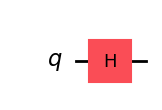
\includegraphics[width=0.25\linewidth]{Images/QH1.png}
% \end{figure}

% \begin{lstlisting}[language=Python]
% # Auxiliary circuit for X
% aux_circuit[0].draw('mpl')
% \end{lstlisting}
% \begin{figure}[ht]
%     \centering
%     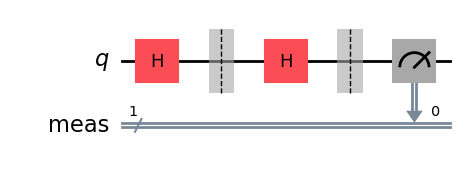
\includegraphics[width=0.5\linewidth]{Images/aux_circ_cost.png}
% \end{figure}

% \begin{lstlisting}[language=Python]
% # Auxiliary circuit for Z
% aux_circuits[1].draw('mpl')
% \end{lstlisting}
% \begin{figure}[ht]
%     \centering
%     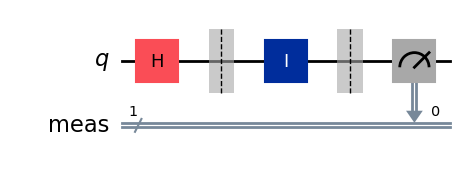
\includegraphics[width=0.5\linewidth]{Images/aux_circ2.png}
% \end{figure}
% We can now carry out the computation manually using Sampler and check the results on Estimator:

% \begin{lstlisting}[language=Python]
% from qiskit.primitives import StatevectorSampler, StatevectorEstimator
% from qiskit.result import QuasiDistribution
% from qiskit.circuit.library import IGate, ZGate, XGate, YGate
% import numpy as np


% ## SAMPLER
% shots = 10000
% sampler = StatevectorSampler()
% job = sampler.run(aux_circuits, shots = shots)
% data_pub = job.result()[1].data
% bitstrings = data_pub.meas.get_bitstrings()
% counts = data_pub.meas.get_counts()
% quasi_dist = QuasiDistribution({outcome: freq / shots for outcome, freq in counts.items()})

% expvals = []
% for pauli in H.paulis:
%     val = 0
    
%     if str(pauli) == "I":
%         Lambda = IGate().to_matrix().real
    
%     if str(pauli) == "X":
%         Lambda = XGate().to_matrix().real
%         val += Lambda[0][1] * quasi_dist.get(1)
%         val += Lambda[1][0] * quasi_dist.get(0)
    
%     if str(pauli) == "Y":
%         Lambda = XGate().to_matrix().real
%         val += Lambda[0][1] * 1.j * quasi_dist.get(1)
%         val += Lambda[1][0] * -1.j * quasi_dist.get(0)

%     if str(pauli) == "Z":
%         Lambda = ZGate().to_matrix().real
%         val += Lambda[0][0] * quasi_dist.get(0)
%         val += Lambda[1][1] * quasi_dist.get(1)
    
%     expvals.append(val)

% print("Sampler results:")
% for (pauli, expval) in zip(H.paulis, expvals):
%     print(f"  >> Expected value of {str(pauli)}: {expval:.5f}")

% total_expval = np.sum(H.coeffs * expvals).real
% print(f"  >> Total expected value: {total_expval:.5f}")

% ## ESTIMATOR
% observables = [
%     *H.paulis,H
% ]  # Note: run for individual Paulis as well as full observable H

% estimator = StatevectorEstimator()
% job = estimator.run([(original_circuit, observables)])
% estimator_expvals = job.result()[0].data.evs

% print("Estimator results:")
% for (obs, expval) in zip(observables, estimator_expvals):
%     if obs is not H:
%         print(f"  >> Expected value of {str(obs)}: {expval:.5f}")
%     else:
%         print(f"  >> Total expected value: {expval:.5f}")
% \end{lstlisting}
% Output:
% \begin{lstlisting}
% Sampler results:
%   >> Expected value of X: 1.00000
%   >> Expected value of Z: 0.00860
%   >> Total expected value: 1.99140
% Estimator results:
%   >> Expected value of X: 1.00000
%   >> Expected value of Z: 0.00000
%   >> Total expected value: 2.00000
% \end{lstlisting}
% \subsubsection{Mathematical rigor}
% Expressing $\ket{\psi}$ with respect to the basis of eigen states of $\hat{H}$,$\ket{\psi}=\sum_{\lambda}a_{\lambda}\ket{\lambda}$, it follows:
% \begin{align*}
% \braket{\psi|\hat{H}|\psi}&=\left(\sum_{\lambda'}a_{\lambda'}^*\bra{\lambda'}\right)\hat{H}\left(\sum_{\lambda}a_{\lambda}\ket{\lambda}\right)\\
% &=\sum_{\lambda}\sum_{\lambda'} a_{\lambda'}^*a_{\lambda} \braket{\lambda'|\hat{H}|\lambda}\\
% &=\sum_{\lambda}\sum_{\lambda'}a_{\lambda'}^*a_{\lambda}\lambda \braket{\lambda'|\lambda}\\
% &=\sum-{\lambda}\sum_{\lambda'}a_{\lambda'}^*a_{\lambda}\lambda\delta_{\lambda,\lambda'}\\
% &=\sum_{\lambda}|a_{\lambda}|^2\lambda\\
% &=\sum_{\lambda}p_{\lambda}\lambda
% \end{align*}
% Since we do not know the eigenvalue or eigenstate of the target observable $\hat{H}$, first we need to consider its diagonalization. given that $\hat{H}$ is hermitian, there exists a unitary transformation such that $\hat{H}=V^{\dagger}\Lambda V^{\dagger}$, where $\Lambda$ is the diagonal eigenvalue matrix, so $\braket{j|\lambda|k}=0 \quad \text{if} \quad j\neq k$, and $\braket{j|\Lambda|j}=\lambda_j$.

% This implies that the expected value can be rewritten as:
% \begin{align*}
%     \braket{\psi|\hat{H}\psi}&=\braket{\psi|V^{\dagger}\Lambda V|\psi}\\
%     &=\braket{\psi|V^{\dagger}\left(\sum_{j=0}^{2^n-1}\ket{j}\bra{j}\right)\Lambda\left(\sum_{k=0}^{2^n-1} \ket{k}\bra{k}\right)V|\psi}\\
%     &=\sum_{j=0}^{2^n-1}\sum_{k=0}^{2^n-1} \braket{\psi|V^{\dagger}|j}\braket{j|\Lambda|k}\braket{k|V|\psi}\\
%     &=\sum_{j=0}^{2^n-1} \braket{\psi|V^{\dagger}|j}\braket{j|\Lambda|j}\braket{j|V|\psi}\\
%     &=\sum_{j=0}^{2^n-1}|\braket{j|V|\psi}|^2\lambda_j
% \end{align*}
% Given that if a system is in the state $\ket{\phi}=V\ket{\psi}$ the probability of measuring $\ket{j}$ is $p_j=|\braket{j|\phi}|^2$, the above expected value can be expressed as:
% \[
% \braket{\psi|\hat{H}|\psi}=\sum_{j=0}^{2^n-1}p_j\lambda_j
% \]
% It is very important to note that the probabilities are taken from the state $V\ket{\psi}$ instead of $\ket{\psi}$. This is why the matrix $V$ is absolutely necessary.

% One might be wondering how to obtain the matrix $V$ and the eigenvalues $\Lambda$. If you already had the eigenvalues, then there would be no need to use a quantum computer since the goal of variational algorithms is to find these eigenvalues of $\hat{H}$.

% Fortunately, there is a way around that: any $2^n \times 2^n$ matrix can be written as a linear combination of $4^n$ tensor products of n Pauli matrices and identities, all of which are both Hermitian and Unitary with known $V$ and $\Lambda$.This is what Runtime's \textbf{Estimator} does internally by decomposing any Operator object into a SparsePauliOp.

% Here the Operators that can be used:

% \begin{table}[ht]
%     \centering
%     \resizebox{\textwidth}{!}{
%     \begin{tabular}{|c|c|c|c|}
%     \hline
%         Operator & $\sigma$ & $V$ & $\Lambda$\\
%         \hline
%         I & $\sigma_0=\begin{pmatrix} 1 & 0 \\ 0 & 1 \end{pmatrix}$ & $V_0=I$ & $\Lambda_0=I=\begin{pmatrix} 1 & 0 \\ 0 & 1 \end{pmatrix}$\\
%         \hline
%         X & $\sigma_1=\begin{pmatrix} 0 & 1 \\ 1 & 0 \end{pmatrix}$ & $V_1=H=\frac{1}{\sqrt{2}}\begin{pmatrix} 1 & 1 \\ 1 & -1 \end{pmatrix}$ & $\Lambda_1 = \sigma_3=\begin{pmatrix} 1 & 0 \\ 0 & -1 \end{pmatrix}$\\
%         \hline
%         Y & $\sigma_2=\begin{pmatrix} 0 & -\iota \\ \iota & 0 \end{pmatrix}$ &$V_2=HS^{\dagger}=\frac{1}{\sqrt{2}}\begin{pmatrix} 1 & 1 \\ 1 & -1 \end{pmatrix}\begin{pmatrix} 1 & 0 \\ 0 & -\iota \end{pmatrix}=\frac{1}{\sqrt{2}}\begin{pmatrix} 1 & -\iota \\ 1 & \iota \end{pmatrix}$ & $\Lambda_2 = \sigma_3=\begin{pmatrix} 1 & 0 \\ 0 & -1 \end{pmatrix}$\\
%         \hline
%         Z & $\sigma_3=\begin{pmatrix} 1 & 0 \\ 0 &-1 \end{pmatrix} $& $V_3=I$ & $\Lambda_3=\sigma_3\begin{pmatrix} 1 & 0 \\ 0 & -1 \end{pmatrix}$\\
%         \hline
%     \end{tabular}
%     }
%     \caption{Operators that can be used}
%     \label{tab:operators_used}
% \end{table}

% So let's rewrite $\hat{H}$ with respect to the Paulis and identities:
% \[
% \hat{H}=\sum_{k_{n-1}=0}^3 \ldots \sum_{k_{0}=0}^3 w_{k_{n-1}\ldots k_0} \sigma_{k_{n-1}} \otimes \ldots \otimes \sigma_{k_0} = \sum_{k=0}^{4^n-1}w_k\hat{P}_k
% \]
% where $k=\sum_{l=0}^{n-1}4^lk_l\equiv k_{n-1}\ldots k_0$ for $k_{n-1},\ldots, k_0 \in \{0,1,2,3\}$ (i.e.base 4), and $\hat{P}_k:=\sigma_{k_{n-1}}\otimes \ldots \otimes \sigma_{k_0}$:
% \begin{align*}
% \braket{\psi|\hat{H}|\psi}&=\sum_{k=0}^{4^n-1}w_k\sum_{j=0}^{2^n-1} |\braket{j|V_k|\psi}|^2 \braket{j|\Lambda_k|j}\\
% &=\sum_{k=0}^{4^n-1}w_k\sum_{j=0}^{2^n-1}p_{kj}\lambda_{kj}
% \end{align*}
% where $V_k=V_{k_{n-1}} \otimes \ldots \otimes V_{k_0}$ and $\Lambda_k:=\Lambda_{k_{n-1}} \otimes \ldots \otimes \Lambda_{k_0}$, such that: $\hat{P}_k=V_k^{\dagger}\Lambda_kV_k$.

% \subsection{Cost functions}
% In general, cost functions are used to describe the goal of a problem and how well a trial state is performing with respect to that goal. This definition can be applied to various examples in chemistry, machine learning, finance, optimization, and so on.

% Let's consider a simple example of finding the ground state of a system. Our objective is to minimize the expectation value of the observable representing energy (Hamiltonian $\hat{\mathcal{H}}$):
% \[
% \min_{\vec{\theta}} \braket{\psi(\vec{\theta})|\hat{\mathcal{H}}|\psi(\vec{\theta})}
% \]
% We can use the Estimator to evaluate the expectation value and pass this value to an optimizer to minimize. If the optimization is successful, it will return a set of optimal parameter values $\vec{\theta}^*$, from which we will be able to construct the proposed solution state $\ket{\psi(\vec{\theta}^*)}$ and compute the observed the expectation value as $C(\vec{\theta}^*)$.

% Notice how we will only be able to minimize the cost function for the limited set of states that we are considering. This leads us to two separate possibilities:
% \begin{itemize}
%     \item \textbf{Our ansatz does not define the solution state across the search pace: } If this is the case, our optimizer will never find the solution, and we need to experiment with other ansatzes that might be able to represent our search space more accurately.
%     \item \textbf{Our optimizer is unable to find this valid solution: }Optimization can be globally defined and locally defined.
% \end{itemize}
% All in all, we will be performing a classical optimization loop but relying on the evaluation of the cost function to a quantum computer. From this perspective, one could think of the optimization as a purely classical endeavor where we call some black-box quantum oracle each time the optimizer needs to evaluate the cost function.

% \begin{lstlisting}[language=Python]
% def cost_func_vqe(params, circuit, hamiltonian, estimator):
%     """Return estimate of energy from estimator

%     Parameters:
%         params (ndarray): Array of ansatz parameters
%         ansatz (QuantumCircuit): Parameterized ansatz circuit
%         hamiltonian (SparsePauliOp): Operator representation of Hamiltonian
%         estimator (Estimator): Estimator primitive instance

%     Returns:
%         float: Energy estimate
%     """
%     pub = (circuit, hamiltonian, params)
%     cost = estimator.run([pub]).result()[0].data.evs

% #    cost = estimator.run(ansatz, hamiltonian, parameter_values=params).result().values[0]
%     return cost
% \end{lstlisting}
% \begin{lstlisting}[language=Python]
% from qiskit.circuit.library import TwoLocal

% observable = SparsePauliOp.from_list([("XX", 1), ("YY", -3)])

% reference_circuit = QuantumCircuit(2)
% reference_circuit.x(0)

% variational_form = TwoLocal(
%     2,
%     rotation_blocks=["rz", "ry"],
%     entanglement_blocks="cx",
%     entanglement="linear",
%     reps=1,
% )
% ansatz = reference_circuit.compose(variational_form)

% theta_list = (2 * np.pi * np.random.rand(1, 8)).tolist()
% #ansatz.assign_parameters(theta_list)
% #print(ansatz.num_parameters)
% ansatz.decompose().draw('mpl')
% \end{lstlisting}
% \begin{figure}[ht]
%     \centering
%     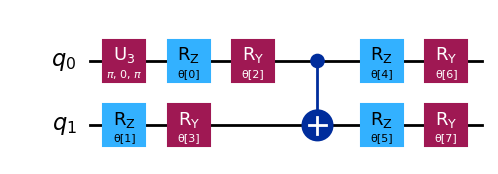
\includegraphics[width=0.5\linewidth]{Images/cost_func_1.png}
% \end{figure}

% We will first carry this out using a simulator: the StatevectorEstimator. This is usually advisable for debugging, but we will immediately follow the debugging run with a calculating on a real quantum hardware. increasingly, problem of interest are no longer classical simulable without state-of-the-art super computing facilities.

% \begin{lstlisting}[language=Python]
% estimator = StatevectorEstimator()
% cost = cost_func_vqe(theta_list, ansatz, observable, estimator)
% print(cost)
% \end{lstlisting}
% \begin{lstlisting}
% [-1.14948565]
% \end{lstlisting}

% We will now proceed with running on real hardware. Note the syntax changes. The steps involving the pass\_manager will be discussed further in the next example.

% \begin{lstlisting}[language=Python]
% #Estimated usage: < 1 min. Benchmarked at 7 seconds on ibm_osaka, 5-23-24
% #Load necessary packages:

% from qiskit_ibm_runtime import QiskitRuntimeService, Session, EstimatorV2 as Estimator
% from qiskit.transpiler.preset_passmanagers import generate_preset_pass_manager

% #Select the least busy backend:

% service = QiskitRuntimeService(channel="ibm_quantum")
% backend = service.least_busy(
%     operational=True, min_num_qubits=ansatz.num_qubits, simulator=False
% )

% #Use a pass manager to transpile the circuit and observable for the specific backend being used:

% pm = generate_preset_pass_manager(backend=backend, optimization_level=1)
% isa_ansatz = pm.run(ansatz)
% isa_observable = observable.apply_layout(layout = isa_ansatz.layout)

% #Open a Runtime session:

% session = Session(backend=backend)

% # Use estimator to get the expected values corresponding to the ansatz

% estimator = Estimator(session=session)
% cost = cost_func_vqe(theta_list, isa_ansatz, isa_observable, estimator)

% # Close session after done
% session.close()
% print(cost)
% \end{lstlisting}
% \begin{lstlisting}
% [-0.79596413]
% \end{lstlisting}

% Note that the values obtained from the two calculations above are very similar. Techniques for improving results will be discussed further below.

% \subsubsection{Example mapping to non-physical systems}
% The maximum cut (Max-Cut) problem is a combinatorial optimization problem that involves dividing the vertices of a graph into two disjoint sets such that the number of edges between the two sets is maximized. More formally, given an undirected graph $G=(V,E)$, where $V$ is the set of vertices and $E$ is the set of edges, the Max-Cut problem asks to partition the vertices into two disjoint subsets, $S$ and $T$, such that the number of edges with one endpoint $S$ and the other in $T$ is maximized.

% We can apply Max-Cut to solve a various problems including: clustering, network design, phase transitions, etc. We'll start by creating a problem graph:
% \begin{lstlisting}[language=Python]
% import rustworkx as rx
% from rustworkx.visualization import mpl_draw

% n = 4
% G = rx.PyGraph()
% G.add_nodes_from(range(n))
% # The edge syntax is (start, end, weight)
% edges = [(0, 1, 1.0), (0, 2, 1.0), (0, 3, 1.0), (1, 2, 1.0), (2, 3, 1.0)]
% G.add_edges_from(edges)

% mpl_draw(G, pos=rx.shell_layout(G), with_labels=True, edge_labels=str, node_color="#1192E8")
% \end{lstlisting}
% \begin{figure}[ht]
%     \centering
%     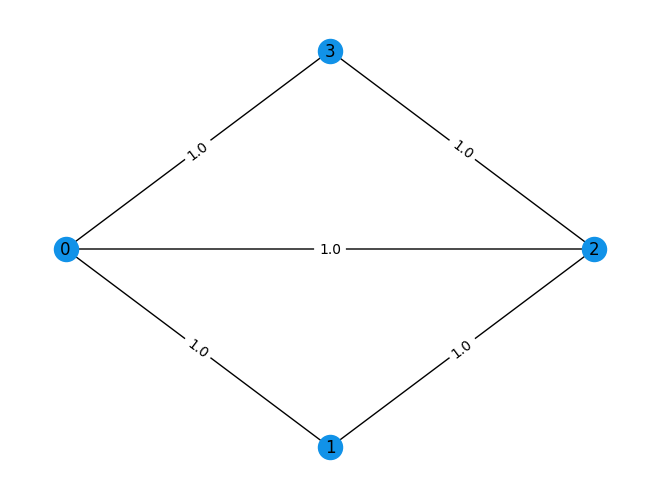
\includegraphics[width=0.5\linewidth]{Images/graph_costexp.png}
% \end{figure}
% This problem can be expressed as a binary optimization problem. For each node $0\leq i<n$, where $n$ is the number of nodes of the graph (in this case $n=4$), we will consider the binary variable $x_i$. This variable will have the value $1$ if node $i$ is one of the groups that we'll label $1$ and $0$ if it's in the other group, that we'll label as 0. We will also denote as $w_{ij}$ (element $(i,j)$ of the adjacency matrix $w$) the weight of the edge that goes from node $i$ to node $j$. because the graph is undirected, $w_{ij}=w_{ji}$. Then we can formulate our problem as maximizing the following cost function:
% \begin{align*}
%     C(\vec{x})&=\sum_{i,j=0}^n w_{ij}x_i(1-x_j)\\
%     &=\sum_{i,j=0}^n w_{ij}x_i-\sum_{i,j=0}^nw_{ij}x_ix_j\\
%     &=\sum_{i,j=0}^n w_{ij}x_i-\sum_{i=0}^n\sum_{j=0}^i 2w_{ij}x_ix_j
% \end{align*}
% To solve this problem with a quantum computer, we are going to express the cost function as the expected value of an observable. However, the observables that Qiskit admits natively consist of Pauli operators, that have eigenvalues $1$ and $-1$ instead of $0$ and $1$. That's why we are going to make the following change of variable:

% Where $\vec{x}=(x_0,x_1,\ldots,x_{n-1})$. We can use the adjacency matrix $w$ to comfortably access the weights of all the edge. This will be used to obtain out cost function:
% \[
%     z_i=1-2x_i\rightarrow x_i=\frac{1-z_i}{2}
% \]
% This implies that:
% \[
% x_i=0\rightarrow z_i=1
% \]
% \[
% x_i=1\rightarrow z_i=-1
% \]
% So the new cost function we want to maximize is:
% \begin{align*}
% C(\vec{z})&=\sum_{i,j=)}^n w_{ij}\left(\frac{1-z_i}{2}\right) \left(1-\frac{1-z_j}{2}\right)\\
% &=\sum_{i,j=0}^n \frac{w_{ij}}{4} - \sum_{i,j=0}^n \frac{w_{ij}}{4}z_iz_j\\
% &=\sum_{i=0}\sum_{j=0}^i \frac{w_{ij}}{2} - \sum_{i=0}^n\sum_{j=0}^i \frac{w_{ij}}{2}z_iz_j
% \end{align*}
% Moreover, the natural tendency of a quantum computer is to find minima (usually the lowest energy) instead of maxima so instead of maximizing $X(\vec{z})$ we are going to minimize:
% \[
% -C(\vec{z})=\sum_{i=0}^n\sum_{j=0}^i \frac{w_{ij}}{2}z_iz_j - \sum_{i=0}\sum_{j=0}^i \frac{w_{ij}}{2}
% \]
% Now that we have a cost function to minimize whose variables can have the values -1 and 1, we can make the following analogy with the Pauli Z:
% \[
% z_i\equiv Z_i=I\otimes \ldots \otimes Z \otimes \ldots \otimes I
% \]
% with $Z$ at the ith position and $I$ everywhere else.

% In other words, the variable $z_i$ will be equivalent to a $Z$ gate acting on qubit i. Moreover:
% \[
% Z_i\ket{x_{n-1}\ldots x_0}=z_i\ket{x_{n-1}\ldots x_0}\rightarrow \braket{x_{n-1}\ldots x_0|Z_i|x_{n-1}\ldots x_0}=z_i
% \]
% Then the observable we are going to consider is:
% \[
% \hat{H}=\sum_{i=0}^n \sum_{j=0}^i \frac{w_{ij}}{2} Z_iZ_j
% \]
% to which we will have to add the independent term afterwards:
% \[
% \text{offset}=-\sum_{i=0}^n\sum_{j=0}^i \frac{w_{ij}}{2}
% \]
% The operator is a linear combination of terms with Z operators on nodes connected by an edge (recall that the 0th qubit is farthest right): $IIZZ+IZIZ+IZZI+ZIIZ+ZZII$. Once the operator is constructed, the ansatz for the QAOA algorithm can easily be built by using the QAOAAnsatz circuit form the Qiskit circuit library.
% \begin{lstlisting}[language=Python]
% from qiskit.circuit.library import QAOAAnsatz
% from qiskit.quantum_info import SparsePauliOp

% hamiltonian = SparsePauliOp.from_list([
%     ("IIZZ", 1), ("IZIZ", 1), ("IZZI", 1), ("ZIIZ", 1), ("ZZII", 1)
% ])


% ansatz = QAOAAnsatz(hamiltonian, reps=2)
% # Draw
% ansatz.decompose(reps=3).draw("mpl")
% \end{lstlisting}
% \begin{figure}[ht]
%     \centering
%     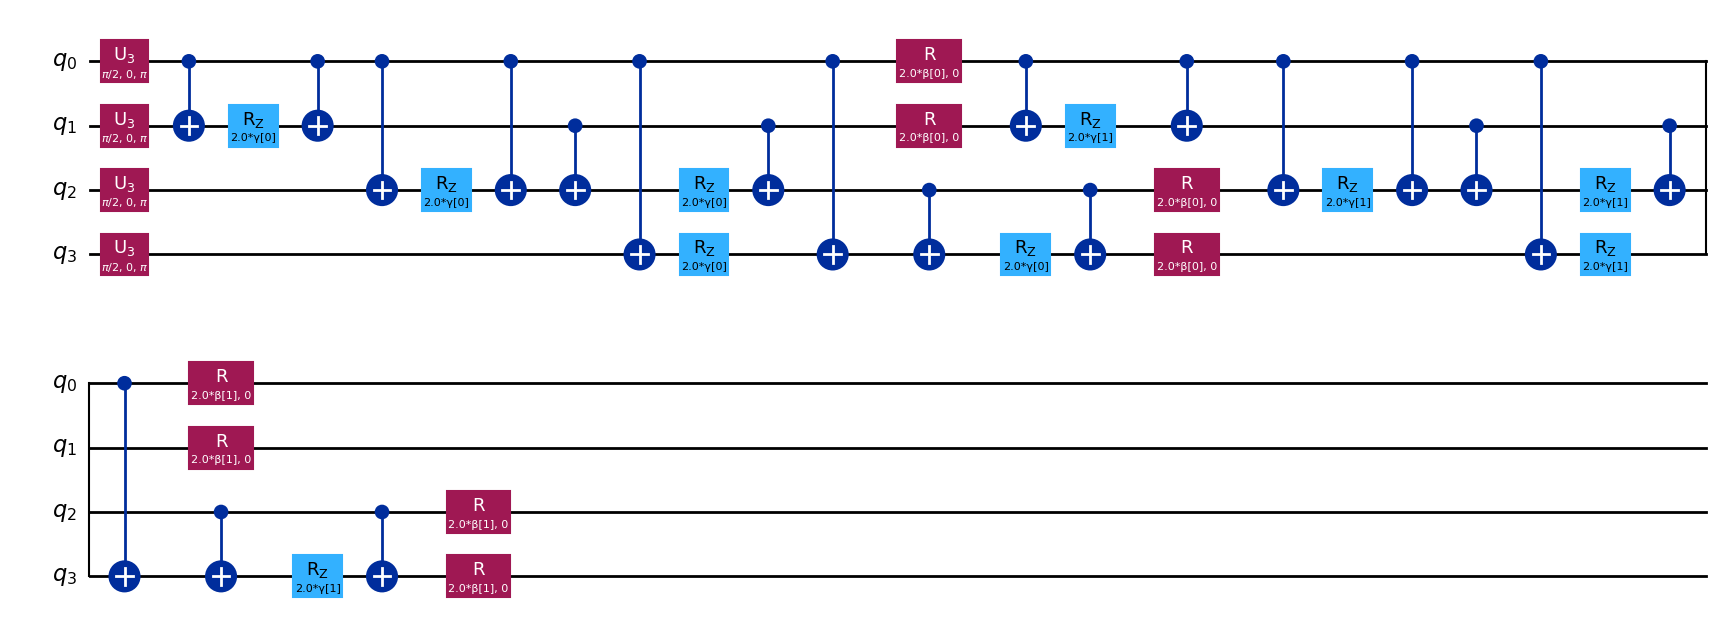
\includegraphics[width=0.75\linewidth]{Images/circ_exp.png}
% \end{figure}

% \begin{lstlisting}[language=Python]
% # Sum the weights, and divide by 2

% offset = - sum(edge[2] for edge in edges) / 2
% print(f"""Offset: {offset}""")
% \end{lstlisting}
% \begin{lstlisting}
% Offset: -2.5
% \end{lstlisting}
% With the Runtime Estimator directly taking a Hamiltonian and parameterized ansatz, and returning the necessary energy, The cost function for a QAOA instance is quite simple:
% \begin{lstlisting}[language=Python]
% def cost_func(params, ansatz, hamiltonian, estimator):
%     """Return estimate of energy from estimator

%     Parameters:
%         params (ndarray): Array of ansatz parameters
%         ansatz (QuantumCircuit): Parameterized ansatz circuit
%         hamiltonian (SparsePauliOp): Operator representation of Hamiltonian
%         estimator (Estimator): Estimator primitive instance

%     Returns:
%         float: Energy estimate
%     """
%     pub = (ansatz, hamiltonian, params)
%     cost = estimator.run([pub]).result()[0].data.evs
% #    cost = estimator.run(ansatz, hamiltonian, parameter_values=params).result().values[0]
%     return cost
% \end{lstlisting}
% \begin{lstlisting}[language=Python]
% import numpy as np

% x0 = 2 * np.pi * np.random.rand(ansatz.num_parameters)

% estimator = StatevectorEstimator()
% cost = cost_func_vqe(x0, ansatz, hamiltonian, estimator)
% print(cost)    
% \end{lstlisting}
% \begin{lstlisting}
% 3.1377748463972157
% \end{lstlisting}
% \begin{lstlisting}[language=Python]
% #Estimated usage: < 1 min, benchmarked at 6 seconds on ibm_osaka, 5-23-24
% #Load some necessary packages:

% from qiskit_ibm_runtime import QiskitRuntimeService
% from qiskit_ibm_runtime import Session, EstimatorV2 as Estimator

% #Select the least busy backend:

% backend = service.least_busy(
%     operational=True, min_num_qubits=ansatz.num_qubits, simulator=False
% )

% #Use a pass manager to transpile the circuit and observable for the specific backend being used:

% pm = generate_preset_pass_manager(backend=backend, optimization_level=1)
% isa_ansatz = pm.run(ansatz)
% isa_hamiltonian = hamiltonian.apply_layout(layout = isa_ansatz.layout)

% #Open a Runtime session:

% session = Session(backend=backend)

% # Use estimator to get the expected values corresponding to each ansatz
% estimator = Estimator(session=session)

% cost = cost_func_vqe(x0, isa_ansatz, isa_hamiltonian, estimator)

% # Close session after done
% session.close()
% print(cost)
% \end{lstlisting}
% \begin{lstlisting}
% 1.8429589920081832
% \end{lstlisting}
% We will revisit this example in Applications to explore how to leverage an optimizer to iterate through the search space. Generally, speaking, this includes:
% \begin{itemize}
%     \item Leveraging an optimizer to find optimal parameters
%     \item Binding optimal parameters to the ansatz to find the eigenvalues
%     \item Translating the eigenvalues to our problem definition
% \end{itemize}

% \subsubsection{Measurement Strategy: speed vs accuracy}
% As mentioned, we are using noisy quantum computer as a black box oracle, where noise can make the retrieved values non-deterministic, leading to random fluctuations which, in turn, will harm - or even completely prevent the convergence of certain optimizers to a proposed solution. This is a general problem that we must address as we incrementally explore quantum utility and progress towards quantum advantage:
% \begin{figure}[ht]
%     \centering
%     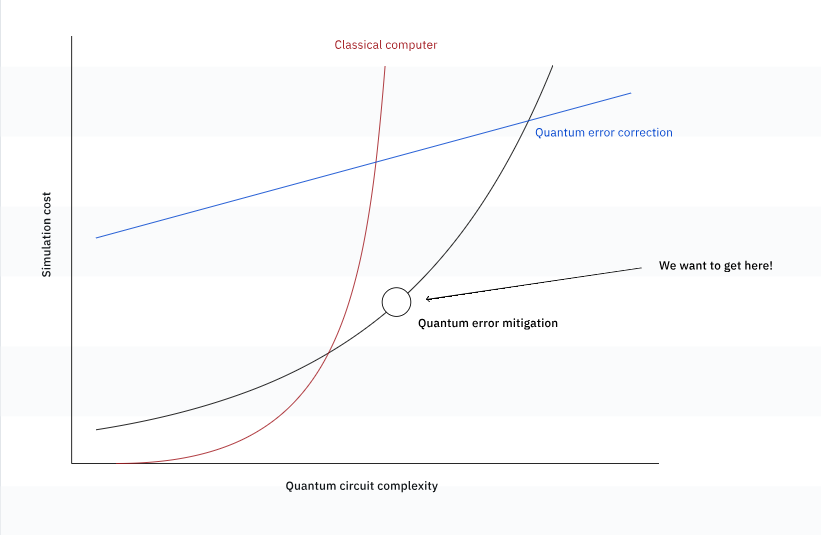
\includegraphics[width=1\linewidth]{Images/measstrat_speedvsacc.png}
% \end{figure}
% We can use Qiskit Runtime Primitive's error suppression and error mitigation options to address noise and maximize the utility of today's quantum computers.

% \subsubsection{Error Suppression}
% Error suppression refers to techniques used to optimize and transform a circuit during compilation in order to minimize errors. This is a basic error handling technique that usually results in some classical pre-processing overhead to the overall runtime. The overhead includes transpiling circuits to run on a quantum hardware by:
% \begin{itemize}
%     \item Expressing the circuit using the native gates available on a quantum system.
%     \item Mapping the virtual qubits to physical qubits
%     \item Adding SWAPs based on connectivity requirements
%     \item Optimizing 1Q and 2Q gates
%     \item Adding dynamical decoupling to idle qubits to prevent the effects of decoherence.
% \end{itemize}
% Primitives allow for the use of error suppression techniques by setting the optimization\_level option and selecting advanced transpilation options. Later, we will delve into different circuit construction methods to improve results, but for most cases, we recommend setting optimization\_level=3.

% We will visualize the value of increasing optimization in the transpilation process by looking at an example circuit with simple ideal behaviour.
% \begin{lstlisting}[language=Python]
% from qiskit.circuit import Parameter, QuantumCircuit
% from qiskit.quantum_info import SparsePauliOp

% theta = Parameter("theta")

% qc = QuantumCircuit(2)
% qc.x(1)
% qc.h(0)
% qc.cp(theta, 0, 1)
% qc.h(0)
% observables = SparsePauliOp.from_list([("ZZ", 1)])

% qc.draw("mpl")
% \end{lstlisting}
% \begin{figure}[ht]
%     \centering
%     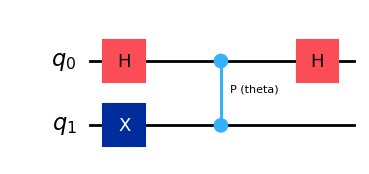
\includegraphics[width=0.5\linewidth]{Images/err_sup_circ.png}
% \end{figure}
% The circuit above can yield sinusoidal expectation values of the observable given, provided we insert phases spanning an appropriate interval, such as $[0,2\pi]$.
% \begin{lstlisting}[language=Python]
% ## Setup phases
% import numpy as np

% phases = np.linspace(0, 2*np.pi, 50)

% # phases need to be expressed as a list of lists in order to work
% individual_phases = [[phase] for phase in phases]
% \end{lstlisting}

% We can uses a simulator to show the usefulness of an optimized transpilation. We will return below to using real hardware to demonstrate the usefulness of error mitigation. We will use QiskitRuntime Service to get a real backend (in this case, ibm\_kyoto), and use AerSimulator to simulate that backend, including its noise behavior.
% \begin{lstlisting}[language=Python]
% from qiskit_ibm_runtime import QiskitRuntimeService
% from qiskit_aer import AerSimulator

% # get a real backend from the runtime service
% service = QiskitRuntimeService()
% backend = service.get_backend('ibm_sherbrooke')
 
% # generate a simulator that mimics the real quantum system with the latest calibration results
% backend_sim = AerSimulator.from_backend(backend)
% \end{lstlisting}
% We can now use a pass manager to transpile the circuit into the "instruction set architecture" or ISA of the backend. This is a new requirement in Qiskit Runtime: all circuits submitted to a backend must conform to the constraints of the backend's target, meaning they must be written in terms of the backend's ISA - i.e., the set of instructions the device can understand and execute. These target constraints are defined by factors like the device's native basis gates, its qubit connectivity, and - when relevant - its pulse and other instruction timing specifications.

% Note that in the present case, we will do this twice: once with optimization\_level=0, and once with it set to 3. Each time we will use the Estimator primitive to estimate the expectation values of the observable at different values of phase.

% \begin{lstlisting}[language=Python]
% #Import estimator and specify that we are using the simulated backend:

% from qiskit_ibm_runtime import EstimatorV2 as Estimator
% estimator = Estimator(backend = backend_sim)

% circuit = qc

% #Use a pass manager to transpile the circuit and observable for the backend being simulated.
% #Start with no optimization:

% from qiskit.transpiler.preset_passmanagers import generate_preset_pass_manager

% pm = generate_preset_pass_manager(backend=backend_sim, optimization_level=0)
% isa_circuit = pm.run(circuit)
% isa_observables = observables.apply_layout(layout = isa_circuit.layout)

% noisy_exp_values = []
% pub = (isa_circuit, isa_observables, [individual_phases])
% cost = estimator.run([pub]).result()[0].data.evs
% noisy_exp_values = cost[0]

% #Repeat above steps, but now with optimization = 3:

% exp_values_with_opt_es = []
% pm = generate_preset_pass_manager(backend=backend_sim, optimization_level=3)
% isa_circuit = pm.run(circuit)
% isa_observables = observables.apply_layout(layout = isa_circuit.layout)

% pub = (isa_circuit, isa_observables, [individual_phases])
% cost = estimator.run([pub]).result()[0].data.evs
% exp_values_with_opt_es = cost[0]
% \end{lstlisting}

% Finally, we can plot the results, and we see that the precision of the calculation was fairly good even without optimization, but it definitely improved by increasing the optimization to level 3. Note that in deeper, more complicated circuits, the difference between optimization levels of 0 and 3 are likely to be more signification. This is a very simple circuit used as a toy model.

% \begin{lstlisting}[language=Python]
% import matplotlib.pyplot as plt

% plt.plot(phases, noisy_exp_values, "o", label="opt=0")
% plt.plot(phases, exp_values_with_opt_es, "o", label="opt=3")
% plt.plot(phases, 2 * np.sin(phases / 2) ** 2 - 1, label="ideal")
% plt.ylabel("Expectation")
% plt.legend()
% plt.show()
% \end{lstlisting}

% \subsubsection{Error Mitigation}
% Error mitigation refers to techniques that allow users to reduce circuit errors by modelling the device noise at the time of execution. Typically, this results in quantum pre-processing overhead related to model training and classical post-processing overhead to mitigate errors in the raw results by using the generated model.

% The Qiskit Runtime primitive's resilience\_level option specifies the amount of resilience to build against errors. Higher levels generate more accurate results at the expense of longer processing times due  to quantum sampling overhead. Resilience levels can be used to configure the trade-off between cost and accuracy when applying error mitigation to your primitive query.

% When implementing any error mitigation technique, we expect the bias in our results to be reduced with respect to the previous, unmitigated bias. In some cases, the bias may even disappear. However, this comes at a cost. As we reduce the bias in our estimated quantities, the statistical variability will increase (that is, variance), which can account for further increasing the number of shots per circuit in our sampling process. This will introduce overhead beyond that needed to reduce the bias, so it is not done by default. We can easily opt-in to this behavior by adjusting the number of shots per circuit in options.executions.shots, as shown in the example below.

% \begin{figure}[ht]
%     \centering
%     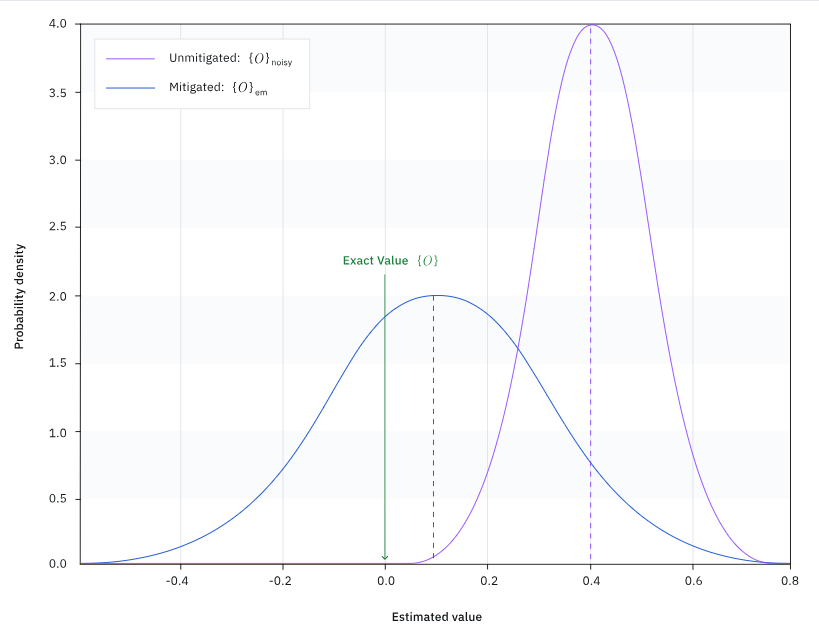
\includegraphics[width=\linewidth]{Images/error_miti.png}
% \end{figure}

% We will now explore these error mitigation models at high level to illustrate the error mitigation that Qiskit Runtime primitives can perform without requiring full implementation details. 

% \subsubsection{Twirled readout error extinction (T-REx)}
% Twirled readout error extinction (T-REx) uses a technique known as Pauli twirling to reduce the noise introduced during the process of quantum measurement. This technique assumes no specific form of noise, which makes it very general and effective.

% Overall workflow:
% \begin{enumerate}
%     \item Acquire data for the zero state with randomized bit flips (Pauli X before measurement)
%     \item Acquire data for the desired (noisy) state with randomized bit flips (Pauli X before measurement)
%     \item Compute the special function for each data set, and divide.
% \end{enumerate}

% \begin{figure}[ht]
%     \centering
%     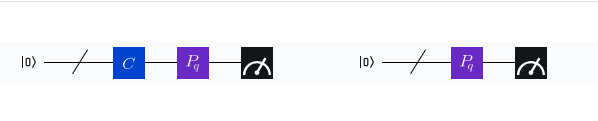
\includegraphics[width=0.75\linewidth]{Images/fig_Trex.png}
% \end{figure}
% We can set this with options.resilience\_level=1, demonstrated in the example below.

% \subsubsection{Zero noise extrapolation}
% Zero noise extrapolation (ZNE) works by first amplifying the noise in the circuit that is preparing the desired quantum state, obtaining measurements for several different levels of noise, and using those measurements to infer the noiseless result.

% Overall workflow:
% \begin{enumerate}
%     \item Amplify circuits noise for several noise factors.
%     \item Run every noise amplifies circuit
%     \item Extrapolate back to the zero noise limit.
% \end{enumerate}

% \begin{figure}[ht]
%     \centering
%     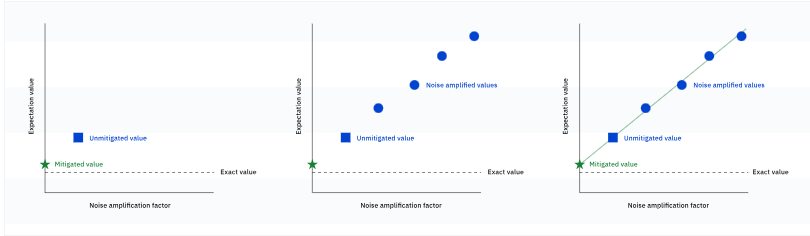
\includegraphics[width=0.5\linewidth]{Images/zne.png}
% \end{figure}

% we can set this with options.resilience\_level=2. We can optimize this further by exploring a variety of noise\_factors, noise\_amplifiers, and extrapolators, but this is outside the scope of this. We encourage you to experiment with this options.

% Each method comes with its own associated overhead: a trage-off between the number of quantum computations needed (time) and the accuracy of the results:

% \begin{table}[ht]
%     \centering
%     \begin{tabular}{c|c|c}
%     Methods & R=1, T-REx & R=2, ZNE \\
%     \hline
%     Assumptions  & None & Ability to scale noise\\
%          Qubit overhead &  1  &  1\\
%          Sampling overhead& 2 & $N_{noise-factors}$\\
%          Bias & 0 & $\mathcal{O}(\lambda^N_{noise-factors})$\\
%     \end{tabular}
%     \caption{Caption}
%     \label{tab:my_label}
% \end{table}

% \subsubsection{Using Qiskit Runtime's mitigation and suppression options}
% Here's how to calculate an expectation value while using error mitigation and suppression in Qiskit Runtime. We can make use of precisely the same circuit and observable as before, but this time keeping the optimization level fixed at level 2, and now tuning the resilience or the error mitigation techniques beign used. This error mitigation process occurs multiple times throughout an optimization loop.

% We perform this part on real hardware, since error mitigation is not available on simualtors.
% \begin{lstlisting}[language=Python]
% # Estimated usage: 8 minutes, benchmarked on ibm_sherbrooke, 5-23-24

% from qiskit_ibm_runtime import QiskitRuntimeService
% from qiskit_ibm_runtime import Options, Session, EstimatorV2 as Estimator

% # We select the least busy backend

% backend = service.least_busy(
%     operational=True, min_num_qubits=ansatz.num_qubits, simulator=False
% )

% #Initialize some variables to save the results from different runs:

% exp_values_with_em0_es = []
% exp_values_with_em1_es = []
% exp_values_with_em2_es = []

% #Use a pass manager to optimize the circuit and observables for the backend chosen:

% pm = generate_preset_pass_manager(backend=backend, optimization_level=2)
% isa_circuit = pm.run(circuit)
% isa_observables = observables.apply_layout(layout = isa_circuit.layout)

% # Open a session and run with no error mitigation:

% with Session(backend=backend) as session:
%     session_options = Options()
%     session_options.execution.shots = 2000
%     session_options.resilience_level = 0

%     estimator = Estimator(session=session)
%     estimator.options.default_shots = 10_000
    
%     pub = (isa_circuit, isa_observables, [individual_phases])
%     cost = estimator.run([pub]).result()[0].data.evs

% session.close()

% exp_values_with_em0_es = cost[0]

% # Open a session and run with resilience = 1:

% with Session(backend=backend) as session:
%     session_options = Options()
%     session_options.execution.shots = 2000
%     session_options.resilience_level = 1

%     estimator = Estimator(session=session)
%     estimator.options.default_shots = 10_000
    
%     pub = (isa_circuit, isa_observables, [individual_phases])
%     cost = estimator.run([pub]).result()[0].data.evs

% session.close()

% exp_values_with_em1_es = cost[0]

% # Open a session and run with resilience = 2:

% with Session(backend=backend) as session:
%     session_options = Options()
%     session_options.execution.shots = 2000
%     session_options.resilience_level = 2

%     estimator = Estimator(session=session)
%     estimator.options.default_shots = 10_000
    
%     pub = (isa_circuit, isa_observables, [individual_phases])
%     cost = estimator.run([pub]).result()[0].data.evs

% session.close()

% exp_values_with_em2_es = cost[0]
% \end{lstlisting}
% As before, we can plot the resulting expectation values as a function of phase angles for the three levels of error mitigation used. With great difficult, one can see that error mitigation improves the results slightly. Again, this effect is much more pronounced in deeper, more complicated circuits.

% \begin{lstlisting}[language=Python]
% import matplotlib.pyplot as plt

% plt.plot(phases, exp_values_with_em0_es, "o", label="unmitigated")
% plt.plot(phases, exp_values_with_em1_es, "o", label="resil = 1")
% plt.plot(phases, exp_values_with_em2_es, "o", label="resil = 2")
% plt.plot(phases, 2 * np.sin(phases / 2) ** 2 - 1, label="ideal")
% plt.ylabel("Expectation")
% plt.legend()
% plt.show()
% \end{lstlisting}
% \begin{figure}[ht]
%     \centering
%     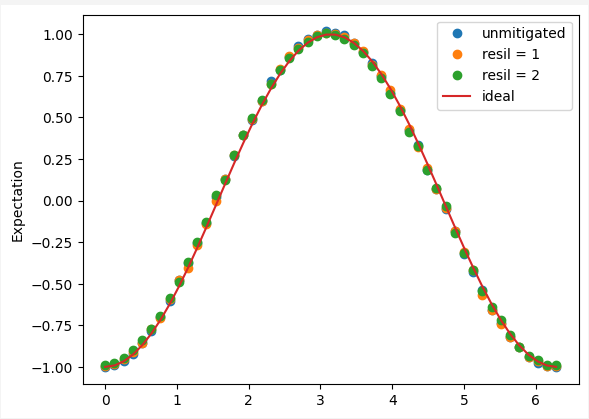
\includegraphics[width=0.75\linewidth]{Images/zne-plot.png}
% \end{figure}
% \subsection{Summary}
% With this lesson, you learned how to create a cost function:
% \begin{itemize}
%     \item Create a cost function
%     \item How to leverage Qiskit Runtime primitives to mitigate and suppression noise
%     \item how to define a measurement strategy to optimize speed vs accuracy
% \end{itemize}
% Here's high-level variational workload:
% \begin{figure}[ht]
%     \centering
%     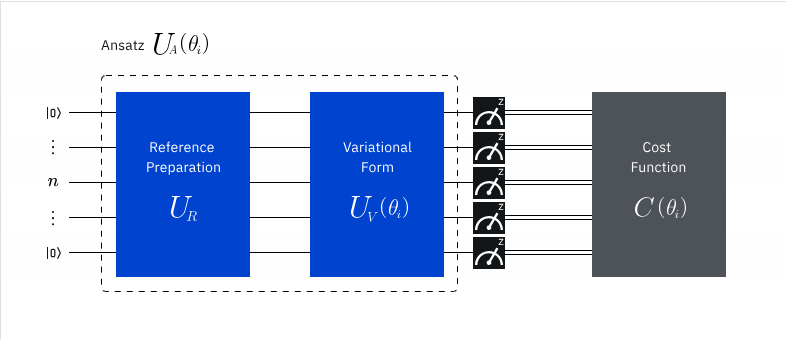
\includegraphics[width=0.75\linewidth]{Images/summ_cost.png}
% \end{figure}
% Our cost function runs during every iteration of the optimization loop. The next lesson will explore how the classical optimizer uses our cost function evaluation to select new parameters.
% \begin{lstlisting}[language=Python]
% import qiskit
% import qiskit_ibm_runtime
% print(qiskit.version.get_version_info())
% print(qiskit_ibm_runtime.version.get_version_info())
% \end{lstlisting}
% \begin{lstlisting}
% 1.2.0
% 0.28.0
% \end{lstlisting}

% \section{Optimization Loops}
% Now we will see how to use an optimizer to iteratively explore the parameterized quantum states of our ansatz:
% \begin{itemize}
%     \item Bootstrap an optimization loop
%     \item understand trade-offs while using local and global optimizers
%     \item Explore barren plateaus and how to avoid them
% \end{itemize}
% At a high level, optimizers are central to exploring our search space. the optimizer uses cost function evaluations to select the next set of parameters in a variational loop, and repeats the process until it reaches a stable state. At this stage, an optimal set of parameter values $\vec{\theta}^*$ is returned.
% \begin{figure}[ht]
%     \centering
%     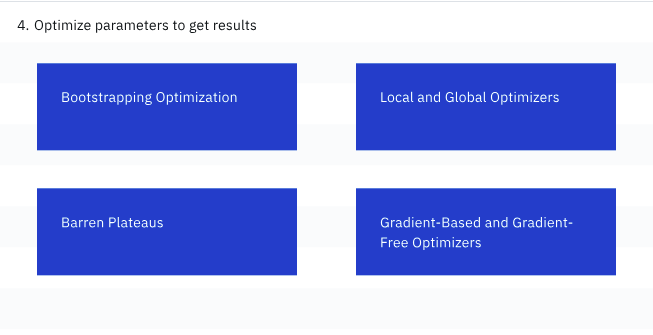
\includegraphics[width=0.75\linewidth]{Images/Opti_loops_vqe.png}
% \end{figure}
% \subsection{Local and Global Optimizers}
% We will first setup our problem before exploring each optimizer class:
% \begin{lstlisting}[language=Python]
% from qiskit import QuantumCircuit
% from qiskit.quantum_info import SparsePauliOp
% from qiskit.circuit.library import TwoLocal
% import numpy as np

% theta_list = (2 * np.pi * np.random.rand(1, 8)).tolist()
% observable = SparsePauliOp.from_list([("XX", 1), ("YY", -3)])

% reference_circuit = QuantumCircuit(2)
% reference_circuit.x(0)

% variational_form = TwoLocal(
%     2,
%     rotation_blocks=["rz", "ry"],
%     entanglement_blocks="cx",
%     entanglement="linear",
%     reps=1,
% )
% ansatz = reference_circuit.compose(variational_form)

% ansatz.decompose().draw('mpl')
% \end{lstlisting}
% \begin{figure}[ht]
%     \centering
%     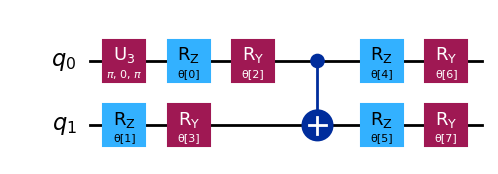
\includegraphics[width=1\linewidth]{Images/ansatz_oplopps.png}
% \end{figure}
% \begin{lstlisting}[language=Python]
% def cost_func_vqe(params, ansatz, hamiltonian, estimator):
% """Return estimate of energy from estimator

% Parameters:
%     params (ndarray): Array of ansatz parameters
%     ansatz (QuantumCircuit): Parameterized ansatz circuit
%     hamiltonian (SparsePauliOp): Operator representation of Hamiltonian
%     estimator (Estimator): Estimator primitive instance

% Returns:
%     float: Energy estimate
% """
% pub = (ansatz, hamiltonian, params)
% cost = estimator.run([pub]).result()[0].data.evs
% return cost
% \end{lstlisting}
% \begin{lstlisting}[language=Python]
% from qiskit.primitives import StatevectorEstimator
% estimator = StatevectorEstimator()
% \end{lstlisting}



% \subsubsection{Local Optimizers}
% Local optimizers search for a point that minimizes the cost function starting at an initial point(s) $C(\vec{\theta}_0)$ and move to different points based on what they observe in the region they are currently evaluation on successive iterations. This implies that the convergence of these algorithms  will usually be fast, but can be heavily dependent on the initial point. Local optimizers are unable to see beyond the region where they are evaluating and can be especially vulnerable to local minima, reporting convergence when they find one and ignoring other states with more favorable evaluations.

% \begin{lstlisting}[language=Python]
% # SciPy minimizer routine
% from scipy.optimize import minimize

% x0 = np.ones(8)

% result = minimize(cost_func_vqe, x0, args=(ansatz, observable, estimator), method="SLSQP")

% result
% \end{lstlisting}
% \begin{lstlisting}
% message: Optimization terminated successfully
%  success: True
%   status: 0
%      fun: -3.99999999645274
%        x: [ 1.000e+00  1.000e+00 -1.571e+00 -4.556e-05 -1.207e+00
%            -1.935e+00  4.079e-01 -4.079e-01]
%      nit: 12
%      jac: [ 1.192e-07  2.980e-08 -7.959e-04  2.543e-04  1.381e-03
%             1.381e-03  5.431e-04  5.431e-04]
%     nfev: 112
%     njev: 12
% \end{lstlisting}

% \subsubsection{Global Optimizers}
% Global optimizers search for the point that minimizes the cost function over several regions of its domain (i.e. non-local), evaluating it iteratively (i.e. at iteration $i$) over a set of parameters vectors $\Theta_i = \vec{\theta}_{i,j}|\in \mathcal{J}_{opt}^i$ determined by the optimizer. This makes them less susceptible to local minima and somewhat independent of initialization, but also significantly slower to converge to a proposed solution.

% \subsubsection{Bootstrapping Optimization}
% Bootstrapping, or setting the initial value for parameters $\vec{\theta}$ based on a prior optimization, can help our optimizer converge on a solution faster. we refer to this as the initial point $\vec{\theta}_0$, and $\ket{\psi(\vec{\theta}_0)}=U_V(\vec{\theta}_0)\ket{\rho}$ as the initial state. This initial state differs from our reference state $\ket{\rho}$, as the former focuses on initial parameters set during our optimization loop, while the latter focuses on using known ``reference"solutions> They may coincide if $U_V(\vec{\theta}_0)=I$ (i.e.,the Identity operation).

% When local optimizers converge to non-optimal local minima, we can try bootstrapping the optimization globally and refine the convergence locally. While this requires setting up two variational workloads, it allows the optimizer to find a more optimal solution than the local optimizer alone.

% \subsection{Gradient-Based and Gradient-Free Optimizers}
% \subsubsection{Gradient-Based}
% Four our cost function $C(\vec{\theta})$, if we have access to the gradient of the function $\vec{\nabla}C(\vec{\theta})$ starting from a initial point, the simplest way to minimize the function is to update the parameters towards the direction of steepest descent of the function. That is, we update the parameters as $\vec{\theta}_{n+1}=\vec{\theta}_n-\eta \vec{\nabla}C(\vec{\theta})$, where $\eta$ is the learning rate - a small, positive hyperparameter that controls the size of the update. We continue doing this until we converge to a local minimum of the cost function, $C(\vec{\theta}^*)$. 

% We can use this cost function and an optimizer to calculate optimal parameters.
% \begin{lstlisting}[language=Python]
% # SciPy minimizer routine
% from scipy.optimize import minimize

% x0 = np.ones(8)

% result = minimize(cost_func_vqe, x0, args=(ansatz, observable, estimator), method="BFGS")

% result
% \end{lstlisting}
% \begin{lstlisting}
%  message: Optimization terminated successfully.
%   success: True
%    status: 0
%       fun: -3.999999999999782
%         x: [ 1.000e+00  1.000e+00  1.571e+00  2.785e-07  2.009e-01
%             -2.009e-01  6.342e-01 -6.342e-01]
%       nit: 14
%       jac: [ 5.960e-08 -2.980e-08  8.941e-07  1.013e-06  2.086e-07
%              1.490e-07  5.960e-08  5.960e-08]
%  hess_inv: [[ 1.000e+00 -2.999e-08 ... -7.780e-05 -6.011e-05]
%             [-2.999e-08  1.000e+00 ... -3.475e-06 -7.574e-07]
%             ...
%             [-7.780e-05 -3.475e-06 ...  7.242e-01 -2.603e-01]
%             [-6.011e-05 -7.574e-07 ... -2.603e-01  8.180e-01]]
%      nfev: 144
%      njev: 16
% \end{lstlisting}
% The main advantage of this type of optimization are the convergence speed, which can be very slow, and there is no guarantee to achieve the optimal solution.
% \begin{figure}[ht]
%     \centering
%     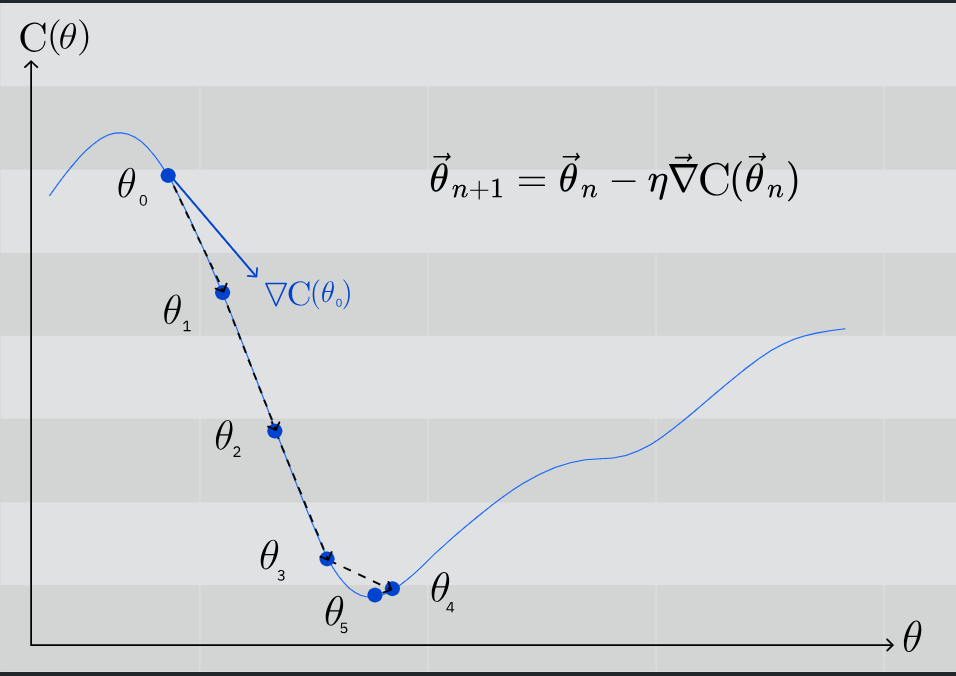
\includegraphics[width=0.75\linewidth]{Images/vqe_grad-based.png}
% \end{figure}
% \subsubsection{Gradient-Free}
% Gradient-free optimization algorithms do not require gradient information and can be useful in situations where computing the gradient is difficult, expensive or too noisy. They also tend to be more robust in finding global optima, whereas gradient based methods tend to converge to local optima. We'll explore a few instance where a gradient-free optimizer can help avoid barren plateaus. However, gradient-free methods require higher computational resources, especially for problems with high-dimensional search spaces.

% Here's an example that uses COBYLA optimizer instead:
% \begin{lstlisting}[language=Python]
% # SciPy minimizer routine
% from scipy.optimize import minimize

% x0 = np.ones(8)

% result = minimize(cost_func_vqe, x0, args=(ansatz, observable, estimator), method="COBYLA")

% result
% \end{lstlisting}
% \begin{lstlisting}
% message: Optimization terminated successfully.
%  success: True
%   status: 1
%      fun: -3.9999999832448676
%        x: [ 1.687e+00  1.250e+00  1.571e+00  3.142e+00  1.469e+00
%            -1.672e+00  1.556e+00  1.585e+00]
%     nfev: 126
%    maxcv: 0.0
% \end{lstlisting}
% \subsection{Barren Plateaus}
% In fact, the cost landscape can be quite complicated, as shown by the hills and valleys in the example below. The optimization method navigates us around the cost landscape, search for the minimum, as shown by the black points and lines. We can see two of the three searches end up in a local minimum of the landscape, rather than a global one.
% \begin{figure}[ht]
%     \centering
%     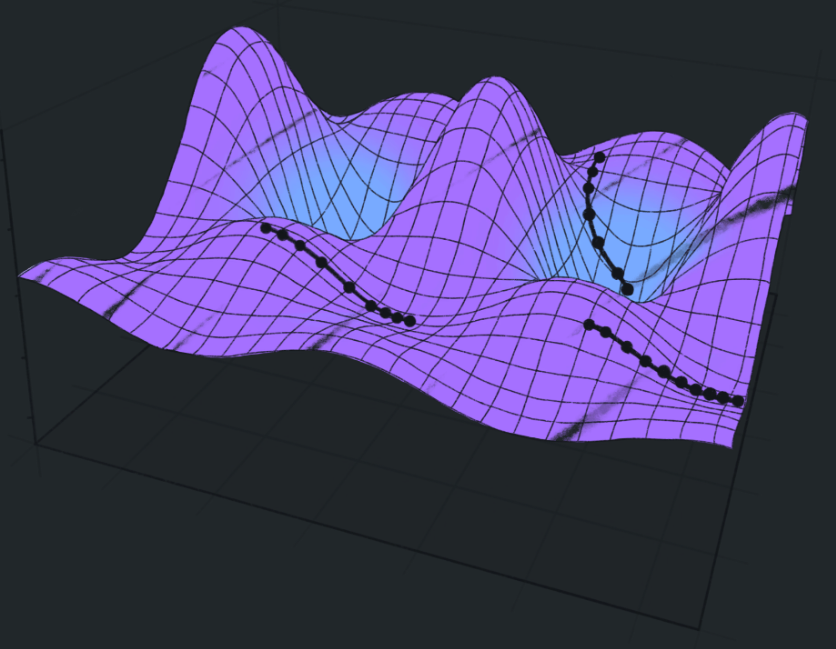
\includegraphics[width=1\linewidth]{Images/vqe_barrenplatuea.png}
% \end{figure}
% Regardless of the type of optimization method used, if the cost landscape is relatively flat, it can be challenging for the method to determine the appropriate direction to search. This scenario is referred to as a barren plateaus, where the cost landscape becomes progressively flatter (and thus more challenging to determine the direction of the minimum). For a broad range of parameterized quantum circuits, the probability that the gradient along any reasonable direction is non-zero to some fixed precision decreases exponentially as the number of qubits increases.
% \begin{figure}[ht]
%     \centering
%     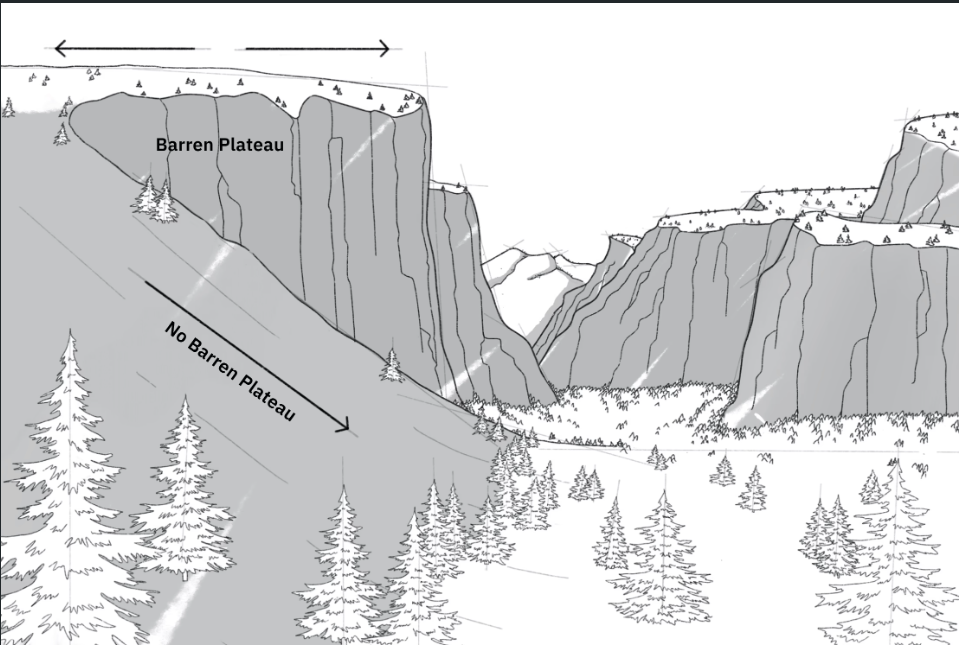
\includegraphics[width=1\linewidth]{Images/vqe_barrenplateaus.png}
% \end{figure}
% Wile this ares is still under active research, we have a few recommendations to improve optimization performance: 
% \begin{itemize}
%     \item \textbf{Bootstrapping}  can help the optimization loop avoid getting stuck in a parameter space where the gradient is small.
%     \item \textbf{Experimenting with hardware-efficient ansatz}: Since we're using a noisy quantum system as a black box oracle, the quality of those evaluations can affect the optimzier's performance. Using hardware-efficient ansatz, such as EfficientSU2, may avoid producing exponentially small gradients.
%     \item \textbf{Experimenting with error suppression and error mitigation}: the Qiskit Runtime primitives provide a simple interface to experiment with various optimization\_level and resilience\_setting respectively. This can be reduced the impact of noise and make the optimization process more efficient.
%     \item \textbf{Experimenting with gradient-free optimizers:} Unlike gradient-based optimization algorithms, optimizers such as COBYLA do not rely on gradient information to optimize the parameters and are therefore less likely to be affected by the barren plateau.
% \end{itemize}
% \subsection{Summary}
% With this lesson, you learned how to define your optimization loop:
% \begin{itemize}
%     \item Bootstrap an optimization loop
%     \item Understand trade-offs while using local and global optimizers
%     \item Explore barren plateaus and how to avoid them
% \end{itemize}
% Our high level variational workload is complete:

% Next, we'll explore specific variational algorithms with this framework in mind.

% \section{Instances and Extensions}
% This chapter will cover several quantum variational algorithms, including:
% \begin{itemize}
%     \item Variational Quantum Eigensolver (VQE)
%     \item Subspace Search VQE (SSVQE)
%     \item Variational Quantum Deflation (VQD)
%     \item Quantum Sampling Regression
% \end{itemize}
% By, using these algorithms, we will learn about several design ideas that can be incorporated into custom variational algorithms, such as weights, penalties, oversampling and undersampling. We encourage you to experiment wit these concepts and share your findings with the community.

% The Qiskit patterns framework applies to all these algorithms - but we will explicitly call out the steps only in the first example.

% \subsection{Variational Quantum eigensolver (VQE)}
% VQE is one of the most widely used variational quantum algorithms, setting up a template for other algorithms to build upon.\\
% \begin{figure}[ht]
%     \centering
%     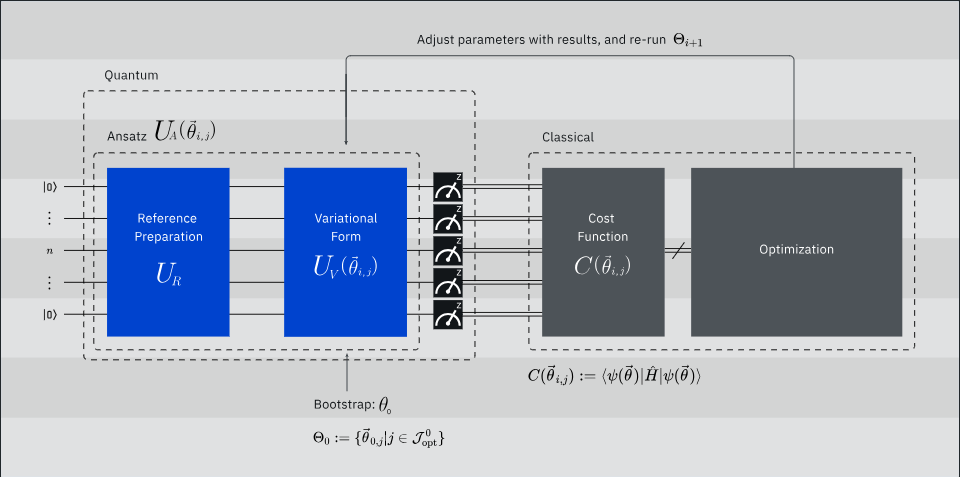
\includegraphics[width=1\linewidth]{Images/vq_img.png}
% \end{figure}
% \textbf{Step 1:} Map classical inputs to a quantum problem

% VQE's theoretical layout is simple:
% \begin{itemize}
%     \item Prepare reference operators $U_R$
%     \item We start from the state $\ket{0}$ and go to the reference state $\ket{\rho}$
%     \item Apply the variational form $U_V(\vec{\theta}_{ij})$ to create an ansatz $U_A(\vec{\theta}_{ij})$
%     \item We go from the state $\ket{\rho}$ to $U_V(\vec{\theta}_{ij})\ket{\rho}=\ket{\psi(\vec{\theta}_{ij})}$
%     \item Bootstrap at $i=0$ if we have a similar problem (typically found via classical simulation or sampling)
%     \item Each optimizer will be bootstrapped differently, resulting in an initial set of parameter vectors $\Theta_0=\vec{\theta}_{0,j}|j\in \mathcal{J}_{opt}^{0}$ (e.g., from an initial point $\vec{\theta}_{0}$).
%     \item Evaluate the cost function $C(\vec{\theta}_{i,j})=\bra{\psi(\vec{\theta})}\hat{H}\ket{\psi(\vec{\theta})}$ for all prepared states on a quantum computer.
%     \item Use a classical optimizer to select the next set of parameters $\Theta_{i+1}$.
%     \item Repeat the process until convergence is reached.
% \end{itemize}
% This is a simple classical optimization loop where we evaluate the cost function. Some optimizers may require multiple evaluations to calculate a gradient, determine the next iteration, or assess convergence.

% Here's the example for the following observable:
% \[
% \hat{O}_1 = 2II - 2XX + 3YY-3ZZ
% \]
% \subsubsection{VQE Implementation}
% \begin{lstlisting}[language=Python]
% from qiskit import QuantumCircuit
% from qiskit.quantum_info import SparsePauliOp
% from qiskit.circuit.library import TwoLocal
% import numpy as np

% theta_list = (2 * np.pi * np.random.rand(1, 8)).tolist()
% observable=SparsePauliOp.from_list([("II", 2), ("XX", -2), ("YY", 3), ("ZZ", -3)])

% reference_circuit = QuantumCircuit(2)
% reference_circuit.x(0)

% variational_form = TwoLocal(
%     2,
%     rotation_blocks=["rz", "ry"],
%     entanglement_blocks="cx",
%     entanglement="linear",
%     reps=1,
% )
% ansatz = reference_circuit.compose(variational_form)

% ansatz.decompose().draw('mpl')
% \end{lstlisting}
% \begin{figure}
%     \centering
%     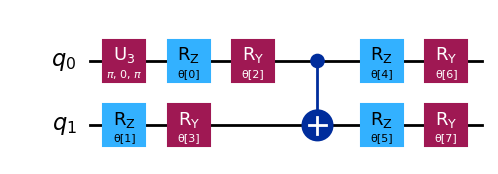
\includegraphics[width=0.75\linewidth]{Images/vqe_impl.png}
% \end{figure}
% \begin{lstlisting}[language=Python]
% def cost_func_vqe(parameters, ansatz, hamiltonian, estimator):
%     """Return estimate of energy from estimator

%     Parameters:
%         params (ndarray): Array of ansatz parameters
%         ansatz (QuantumCircuit): Parameterized ansatz circuit
%         hamiltonian (SparsePauliOp): Operator representation of Hamiltonian
%         estimator (Estimator): Estimator primitive instance

%     Returns:
%         float: Energy estimate
%     """

%     estimator_job = estimator.run([(ansatz, hamiltonian, [parameters])])
%     estimator_result = estimator_job.result()[0]

%     cost = estimator_result.data.evs[0]
%     return cost
% \end{lstlisting}
% \begin{lstlisting}[language=Python]
% from qiskit.primitives import StatevectorEstimator
% estimator = StatevectorEstimator()
% \end{lstlisting}
% We can use this cost function to calculate the optimal parameters
% \begin{lstlisting}[language=Python]
% # SciPy minimizer routine
% from scipy.optimize import minimize

% x0 = np.ones(8)

% result = minimize(cost_func_vqe, x0, args=(ansatz, observable, estimator), method="COBYLA")

% result
% \end{lstlisting}
% \begin{lstlisting}
% message: Optimization terminated successfully.
%  success: True
%   status: 1
%      fun: -5.999999988971083
%        x: [ 1.779e+00  9.443e-01  1.571e+00  2.105e-05  1.938e+00
%             1.204e+00  6.059e-01  6.059e-01]
%     nfev: 136
%    maxcv: 0.0
% \end{lstlisting}
% \textbf{Step2: Optimize problems for quantum execution}
% We will select the least-busy backend, and import the necessary components from the qiskit\_ibm\_runtime.
% \begin{lstlisting}[language=Python]
% from qiskit_ibm_runtime import SamplerV2 as Sampler
% from qiskit_ibm_runtime import EstimatorV2 as Estimator
% from qiskit_ibm_runtime import Session, Options
% from qiskit_ibm_runtime import QiskitRuntimeService


% service = QiskitRuntimeService(channel='ibm_quantum')
% backend = service.least_busy(operational=True, simulator=False)
% \end{lstlisting}
% We will transpile the circuit using the preset pass manager with optimization level 3, and we will apply the corresponding layout to the observable.
% \begin{lstlisting}[language=Python]
% from qiskit.transpiler.preset_passmanagers import generate_preset_pass_manager

% pm = generate_preset_pass_manager(backend=backend, optimization_level=3)
% isa_ansatz = pm.run(ansatz)
% isa_observable = observable.apply_layout(layout = isa_ansatz.layout)
% \end{lstlisting}
% \textbf{Step3: Execute using Qiskit Runtime Primitives}
% We are now ready to run our calculation on IBM Quantum hardware. Because the cost function minimization is highly iterative, we will start at a Runtime session. This way we only have to wait in a queue once. Once the job begins running, each iteration with updates to parameters will run immediately.
% \begin{lstlisting}[language=Python]
% #Estimated required time: <20 min. Benchmarked at 17 min, 40 s on ibm_osaka, on 5-29-24

% x0 = np.ones(8)

% with Session(backend=backend) as session:
%     session_options = Options()
%     session_options.execution.shots = 4096
%     session_options.resilience_level = 1

%     estimator = Estimator(session=session)
%     sampler = Sampler(session = session)
%     estimator.options.default_shots = 10_000
    
%     result = minimize(cost_func_vqe, x0, args=(isa_ansatz, isa_observable, estimator), method="COBYLA")

% session.close()
% print(result)
% \end{lstlisting}
% \begin{lstlisting}
%  message: Optimization terminated successfully.
%  success: True
%   status: 1
%      fun: -5.633934465186281
%        x: [ 1.135e+00  1.712e+00  1.340e+00  9.429e-02  2.175e+00
%             7.089e-01  4.387e-01  5.427e-01]
%     nfev: 90
%    maxcv: 0.0
% \end{lstlisting}
% \textbf{Step4: Post-process, return in classical format}
% We can see that the minimization routine successfully terminated, meaning we reached the default tolerance of the COBYLA classical optimizer. If we require a more precise result, we can specify a smaller tolerance. This may indeed be the case, since the result was several percent off compared to the result obtained by the simulator above.

% The value of $x$ obtained is the current best guess for the parameters that minimize the cost function. If iterating to obtain a higher precision, those values should be used in place of the $x0$ initially used (a vector of ones).

% Finally, we note that the function was evaluated $96$ times in the process of optimization. That might be different from the number of optimization steps, since some optimizers require multiple function evaluations in a single step, such as when estimating a gradient.

% \subsection{Subspace Search VQE (SSVQE)}
% SSVQE is a variant of VQE that allows obtaining the first $k$ eigenvalues of an observable $\hat{H}$ with eigenvalues $\{\lambda_0 ,\lambda_1,\ldots ,\lambda_{N-1}\}$, where $N\geq k$. Without loss of generality, we assume that $\lambda_0<\lambda_1<\ldots <\lambda_{N-1}$, SSVQE introduces a new idea by adding weights to help prioritize optimizing for the term with the largest weight.
% \begin{figure}[ht]
%     \centering
%     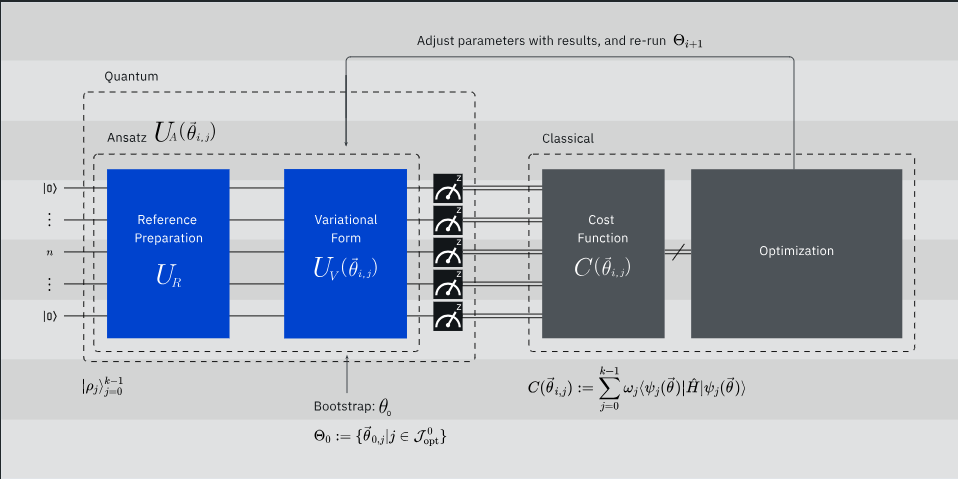
\includegraphics[width=1\linewidth]{Images/ssvqe.png}
% \end{figure}
% To implement this algorithm, we need $k$ mutually orthogonal reference states $\{\ket{\rho_j}\}_{j=0}^{k-1}$, meaning $\braket{\rho_j|\rho_l}=\delta_{jl}$ for $j,l<k$. These states can be constructed using Pauli operators. The cost function of this algorithm is then:
% \begin{align*}
%     C(\vec{\theta})&=\sum_{j=0}^{k-1} w_j \bra{\rho_j}U_V^{\dagger}(\vec{\theta}) \hat{H}U_V(\vec{\theta})\ket{\rho_j}\\
%     &=\sum_{j=0}^{k-1}w_j \bra{\psi_j(\vec{\theta})}\hat{H}\ket{\psi_j(\vec{\theta})}
% \end{align*}
% where $w_j$ is an arbitrary positive number such that if $j<l<k$ then $w_j > w_l$, and $U_V(\vec{\theta})$ is the user-defined variational form.

% The SSVQE algorithm relies on the fact that eigenstates corresponding to different eigenvalues are mutually orthogonal. Specifically, the inner product of $U_V(\vec{\theta})\ket{\rho_j}$ and $U_V(\vec{\theta})\ket{\rho_l}$ can be expressed as:
% \begin{align*}
%     \bra{\rho_j}U_V^{\dagger}(\vec{\theta})U_V(\vec{\theta})\ket{\rho_l}&=\bra{\rho_j}I\ket{\rho_l}\\
%     &=\braket{\rho_j|\rho_l}\\
%     &=\delta_{jl}
% \end{align*}
% The first equality holds because $U_V(\vec{\theta})$ is a quantum operator and is therefore unitary. The last equality holds because of the orthogonality of the reference states $\ket{\rho_j}$. The fact that orthogonality is preserved through unitary transformation is deeply related to the principle of conservation of information, as expressed in quantum information science. Under the view, non -unitary transformations represent processes where information is either lost or injected.

% Weights $w_j$ help ensure that all the states are eigenstates. If the weights are sufficiently different, the term with the largest weight $(i.e., w_0)$ will be given priority during optimization over the others. As a result, the resulting state $U_v(\vec{\theta})\ket{\rho_0}$ will become the eigenstate corresponding to $\lambda_0$. Because $\{U_V(\vec{\theta})\ket{\rho_j}\}_{j=0}^{k-1}$ are mutually orthogonal, the remaining states will be orthogonal to it and, therefore, contained in the subspace corresponding to the eigenvalues $\{\lambda_1,\ldots,\lambda_{N-1}\}$.

% Applying the same argument to the rest of the terms, the next priority would then be the term with weight $w_1$, so $U_V(\vec{\theta})\ket{\rho_l}$ would be the eigenstate corresponding to $\lambda_1$, and the other terms would be contained in the eigenspace of $\{\lambda_2,\ldots,\lambda_{N-1}\}$

% By reasoning inductively, we deduce that $U_V(\vec{\theta})\ket{\rho_j}$ will be an approximate eigenstates of $\lambda_j$ for $0\leq j < k$.

% \subsubsection{SSVQE's Theoretical layout}
% SSVQE's can be summarized as follows:
% \begin{itemize}
%     \item Prepare several reference states by applying a unitary $U_R$ to $k$ different computational basis states
%     \item This algorithm requires the usage of $k$ mutually orthogonal reference states $\{\ket{\rho_j}\}_{j=0}^{k-1}$ such that $\braket{\rho_j|\rho_l}=\delta_{jl}$ for $j,l<k$.
%     \item Apply the variational form $U_V(\vec{\theta}_{i,j})$ to each reference state ,resulting in the following ansatz $U_A(\vec{\theta}_{i,j})$.
%     \item Bootstrap at $i=0$ if a similar problem is available (usually found via classical simulation or sampling.
%     \item Evaluate the cost function $C(\vec{\theta}_{i,j})=\sum_{j=0}^{k-1}w_j\bra{\psi_j(\vec\theta)}\hat{H}\ket{\psi_j(\vec{\theta})}$ for all prepared states on a quantum computer.
%     \item This can be separated into calculating the expectation value for an observable $\bra{\psi_j(\vec{\theta})}\hat{H}\ket{\psi_j(\vec{\theta})}$ and multiplying the result by $w_j$.
%     \item Afterward, the cost function returns the sum of all weighed expectation values.
%     \item Use a classical optimizer to determine the next set of parameters $\Theta_{i+1}$.
%     \item Repeat the above steps until convergence is achieved.
% \end{itemize}
% You will be reconstructing SSVQE's cost function in the assessment, but we have the following snippet to motivate your solution:
% \begin{lstlisting}[language=Python]
% import numpy as np

% def cost_func_ssvqe(params, initialized_anastz_list, weights, ansatz, hamiltonian, estimator):
%     # """Return estimate of energy from estimator

%     # Parameters:
%     #     params (ndarray): Array of ansatz parameters
%     #     initialized_anastz_list (list QuantumCircuit): Array of initialised ansatz with reference
%     #     weights (list): List of weights
%     #     ansatz (QuantumCircuit): Parameterized ansatz circuit
%     #     hamiltonian (SparsePauliOp): Operator representation of Hamiltonian
%     #     estimator (Estimator): Estimator primitive instance

%     # Returns:
%     #     float: Weighted energy estimate
%     # """

%     energies = []

%     # Define SSVQE

%     weighted_energy_sum = np.dot(energies, weights)
%     return weighted_energy_sum
% \end{lstlisting}


% \subsection{Variational Quantum Deflation}
% VQD is an alternative method that extends VQE to obtain the first $k$-eigenvalues of an observable $\hat{H}$ with eigenvalues $\{\lambda_0,\lambda_1,\ldots,\lambda_{N-1}\}$, where $N\geq k$, instead of only the first. For the rest of this section, we will assume, without loss of generality, that $\lambda_0\leq \lambda_1\leq \ldots\leq \lambda_{N-1}$. VQD introduces the notion of a penalty cost to guide the optimization process.
% \begin{figure}[ht]
%     \centering
%     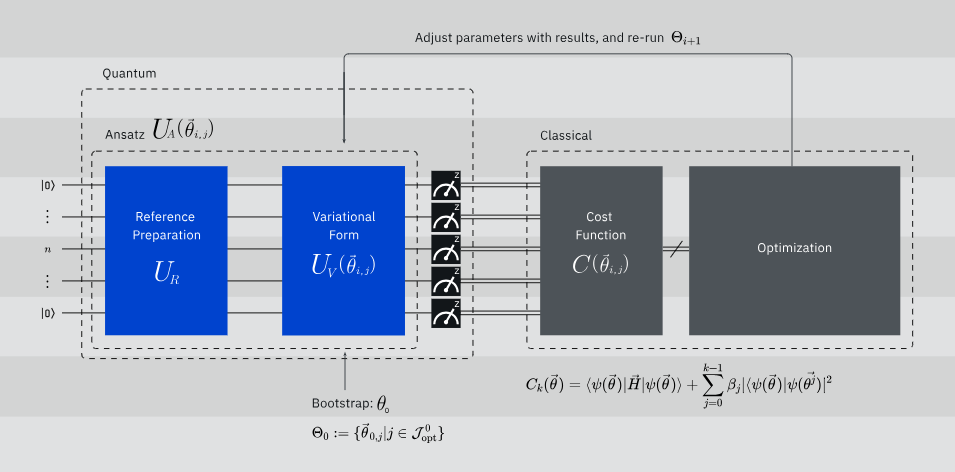
\includegraphics[width=1\linewidth]{Images/vqd_fig.png}
% \end{figure}
% VQD introduces a penalty term, introduced as $\beta$, to balance the contribution of each overlap term to the cost. This penalty term serves to penalize the optimization process if orthogonality is not achieved. We impose this constraint because the eigen states of an observable, or a Hermitian operator, corresponding to different eigenvalues are mutually orthogonal, or can be made so in the case of degeneracy or repeated eigenvalues. Thus, by enforcing orthogonality with the eigenstate corresponding to $\lambda_0$, we are effectively optimizing over the subspace that corresponds to the rest of the eigenvalues $\{\lambda_1,\lambda_2,\ldots,\lambda_{N-1}\}$. here $\lambda_1$ is the lowest eigenvalue from the rest of the eigenvalues and, therefore, the optimal solution to the new problem can be obtained using the variational theorem.

% The general idea behind VQE is to use VQE as usual to obtain the lowest eiegnvalue $\lambda_0=C_0(\vec{\theta}^0)=C_{VQE}(\vec{\theta}^0)$ along with the corresponding (approximate) eigenstate $\ket{\psi(\vec{\theta}^0)}$ for some optimal parameter vector $\vec{\theta}^0$. Then, to obtain the next eigenvalue $\lambda_1>\lambda_0$, instead of minimizing the cost function $C_0(\vec{\theta})=\bra{\psi(\vec{\theta})}\hat{H}\ket{\psi(\vec{\theta})}$, we optimize:
% \[
% C_1(\vec{\theta})=C_0(\vec{\theta})+\beta_0|\braket{\psi(\vec{\theta})|\psi(\vec{\theta}^0)}|^2
% \]
% The positive value $\beta_0$ should be greater than $\lambda_1-\lambda_0$.

% This introduces a new cost function that can be viewd as a constrained problem, where we minimize $C_{VQE}(\vec{\theta})=\bra{\psi(\vec{\theta})}\hat{H}\ket{\psi(\vec{\theta})}$ subject to the constraint that the state must be orthogonal o the previously obtained $\ket{\psi(\vec{\theta}^0})$, with $\beta_0$ acting as a penalty terms if the constraint is not satisfied.

% Alternatively, this new problem can be interpreted as running $VQE$ on the new observable:
% \[
% \hat{H}_1=\hat{H}+\beta_0 \ket{\psi(\vec{\theta}^0)}\bra{\psi(\vec{\theta}^0} \implies C_1(\vec{\theta})=\bra{\psi(\vec{\theta})}\hat{H}_1\ket{\psi(\vec{\theta})},
% \]
% Assuming the solution to the new problem is $\ket{\psi(\vec{\theta}^1)}$, the expected value of $\hat{H}$ (not $\hat{H}_1$) should be $\bra{\psi(\vec{\theta}^1)}\hat{H}\ket{\psi(\vec{\theta}^1)}=\lambda_1$.

% To obtain the third eigenvalue $\lambda_2$, the cost function to optimize is:
% \[
% C_2(\vec{\theta})=C_1(\vec{\theta})+\beta_1|\braket{\psi(\vec{\theta})|\psi(\vec{\theta}^1)}|^2
% \]
% where $\beta_1$ is a positive constant large enough to enforce orthogonality of the solution state to both $\ket{\psi(\vec{\theta}^0)}$ and $\ket{\psi(\vec{\theta}^1)}$. This penalizes states in the search space that do not meet this requirement, effectively restricting the search space. Thus, the optimal solution of the new problem should be the eigenstate corresponding to $\lambda_2$.

% Like the previous case, this new problem can also be interpreted as VQE with the observable:
% \[
% \hat{H}_2=\hat{H}_1+\beta_1\ket{\psi(\vec{\theta}^1)}\bra{\psi(\vec{\theta}^1)}\implies C_2(\vec{\theta}=\bra{\psi(\vec{\theta})}\hat{H}_2\ket{\psi(\vec{\theta})}
% \]
% If the solution to this new problem is $\ket{\psi(\vec{\theta}^2)}$, the expected value of $\hat{H}$ (not $\hat{H}_2$) should be $\bra{\psi(\vec{|theta}^2)}\hat{H}\ket{\psi(\vec{\theta}^2)}=\lambda_2$.

% Analogously, to obtain the $k$th eigenvalue $\lambda_{k-1}$, you would minimize the cost function:
% \[
% C_{k-1}(\vec{\theta})=C_{k-2}(\vec{\theta})+\beta_{k-2}|\braket{\psi(\vec{\theta})|\psi(\vec{\theta}^{k-2})}|^2,
% \]
% Remember that we defined $\vec{\theta}^j$ such that $\bra{\psi(\vec{\theta}^j}\hat{H}\ket{\psi(\vec{\theta}^j}=\lambda_j$, $\forall j <k$. This problem is equivalent to minimizing $V(\vec{\theta})=\bra{\psi(\vec{\theta}}\hat{H}\ket{\psi(\vec{\theta})}$ but with the constraining that the state must be orthogonal to $\ket{\psi(\vec{\theta}^j}$; $\forall j \in 0,\ldots,k-1$, thereby restricting the search space to the subspace corresponding to the eigenvalues $\{\lambda_{k-1},\ldots,\lambda_{N-1}\}$.

% This problem is equivalent to a VQE with the observable:
% \[
% \hat{H}_{k-1}=\hat{H}_{k-2}+\beta_{k-2}\ket{\psi(\vec{\theta}^{k-2})}\bra{\psi(\vec{\theta}^{k-2})}\implies C_{k-1}(\vec{\theta})=\bra{\psi(\vec{\theta})}\hat{H}_{k-1}\ket{\psi(\vec{\theta})},
% \]
% As you can see from the process, to obtain the $k$-th eigenvalue, you need the (approximate) eignestates of the previous $k-1$ eigenvalues, so you would need to run $VQE$ a total of $k$ times. Therefore, VQD's cost function is as follows:
% \[
% C_k(\vec{\theta})=\bra{\psi(\vec{\theta})}\hat{H}\ket{\psi(\vec{\theta})}+\sum_{j=0}^{k-1}\beta_j|\braket{\psi(\vec{\theta})|\psi(\vec{\theta}^j}|^2
% \]
% \subsubsection{VQD's Theoretical Layout}
% VQD's layout can be summarized as follows:
% \begin{itemize}
%     \item Prepare a reference operator $U_R$.
%     \item Apply a variational form $U_V(\vec{\theta}_{i,j})$ to the reference state, creating the following ansatze $U_A(\vec{\theta}_{i,j})$.
%     \item Bootstrap at $i=0$ if we have a similar problem (typically found via classical simulation or sampling)
%     \item Evaluate the cost function $C_k(\vec{\theta})$ which involved computing $k$ excited states and an array of $\beta$'s defining the overall penalty for each overlap term.
%     \item Calculate the expectation value for an observable $\bra{\psi_j(\vec{\theta})}\hat{H}\ket{\psi_j(\vec{\theta})}$ for each $k$
%     \item Calculate the penalty $\sum_{j=0}^{k-1}\beta_j| \braket{\psi(\vec{\theta})|\psi_j(\vec{\theta})}|^2$.
%     \item The cost function should then return the sum of these two terms.
%     \item Use a classical optimizer to choose the next set of parameters $\Theta_{i+1}$
%     \item Repeat this process until convergence is reached.
% \end{itemize}
% \subsubsection{VQD's Implementation}
% For this implementation, we'll create a function for an overlap penalty.This penalty will be used in the cost function at each iteration. This process will be repeated for each excited state
% \begin{lstlisting}[language=Python]
% from qiskit.circuit.library import TwoLocal

% raw_ansatz = TwoLocal(2, rotation_blocks=["ry", "rz"], entanglement_blocks="cz", reps=1)

% raw_ansatz.decompose().draw('mpl')
% \end{lstlisting}
% \begin{figure}[ht]
%     \centering
%     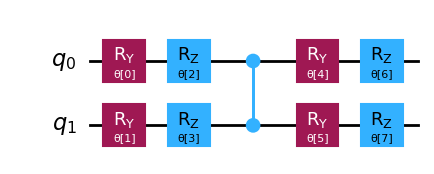
\includegraphics[width=0.75\linewidth]{Images/vqd_circ.png}
% \end{figure}
% First, we'll setup a fuction that calculates the sstate fidelity - a percentage of overlap between two states that we'll use as a penalty for VQD.
% \begin{lstlisting}[language=Python]
% import numpy as np

% def calculate_overlaps(ansatz, prev_circuits, parameters, sampler):

%     def create_fidelity_circuit(circuit_1, circuit_2):

%         """
%         Constructs the list of fidelity circuits to be evaluated.
%         These circuits represent the state overlap between pairs of input circuits,
%         and their construction depends on the fidelity method implementations.
%         """
                
%         if len(circuit_1.clbits) > 0:
%             circuit_1.remove_final_measurements()
%         if len(circuit_2.clbits) > 0:
%             circuit_2.remove_final_measurements()

%         circuit = circuit_1.compose(circuit_2.inverse())
%         circuit.measure_all()
%         return circuit
%     overlaps = []

%     for prev_circuit in prev_circuits:
%         fidelity_circuit = create_fidelity_circuit(ansatz, prev_circuit)
%         sampler_job = sampler.run([(fidelity_circuit, parameters)])
%         meas_data = sampler_job.result()[0].data.meas
        
%         counts_0 = meas_data.get_int_counts().get(0, 0)
%         shots = meas_data.num_shots
%         overlap = counts_0/shots
%         overlaps.append(overlap)
    
%     return np.array(overlaps)
% \end{lstlisting}
% It's time to write VQD's cost function. As before wen we calculated only the ground state, we will determine the lowest energy state using the Estimator primitive. However, as described above, we will now add a penalty term to ensure orthogonality of higher-energy states. That is, for each excited state, a penalty is added for any overlap between the current variational state and the lower-energy eigenstate already found.
% \begin{lstlisting}[language=Python]
% def cost_func_vqd(parameters, ansatz, prev_states, step, betas, estimator, sampler, hamiltonian):

%     estimator_job = estimator.run([(ansatz, hamiltonian, [parameters])])

%     total_cost = 0

%     if step > 1:
%         overlaps = calculate_overlaps(ansatz, prev_states, parameters, sampler)
%         total_cost = np.sum([np.real(betas[state] * overlap) for state, overlap in enumerate(overlaps)])

%     estimator_result = estimator_job.result()[0]

%     value = estimator_result.data.evs[0] + total_cost

%     return value
% \end{lstlisting}
% Note specially that the cost function above refers to the calculate\_overalps function, which actually creates a new quantum circuit. If we want to run on a real hardware, the new circuit must also be transpiled, hopefully in an optimal way, to run on the backend we select. Note that transpilation has been built to the calculate\_overlaps or cost\_func\_vqd functions. Feel free to try modifying the code yourself to build in this additional (and conditional) transpilation - but this will  also be done for you in the next lesson.

% In this lesson, we will run the VQD algorithm using the Statevector Sampler and Statevector Estimator:
% \begin{lstlisting}[language=Python]
% from qiskit.primitives import StatevectorSampler as Sampler
% from qiskit.primitives import StatevectorEstimator as Estimator
% sampler = Sampler()
% estimator = Estimator()
% \end{lstlisting}
% We will introduce an observable to b estimated. In the next lesson we will add some physical context to this, like the excited state of a molecule. It may be helpful to think of this observable as the Hamiltonian of a system that can have excited states, even though this observable has not been chosen to match any particular molecule or atom.
% \begin{lstlisting}[language=Python]
% from qiskit.quantum_info import SparsePauliOp
% observable = SparsePauliOp.from_list([("II", 2), ("XX", -2), ("YY", 3), ("ZZ", -3)])
% \end{lstlisting}
% Here, we set the total number of state we wish to calculate (ground state and excited states, $k$), and the penalties (betas) for overlap between statevectors that should be orthogonal. The consequences of choosing betas to be too high or too low will be explored a bit in the next lesson. For now, we will simply use those provided below. We will start by using all zeros as our parameters. We will start by using all zeros as our parameters. In your own calculations, you may want to use more clever  starting parameters based on your knowledge of the system or on previous calculations.
% \begin{lstlisting}[language=Python]
% k = 3
% betas = [33, 33, 33]
% x0 = np.zeros(8)
% \end{lstlisting}
% We can now run the calculation:
% \begin{lstlisting}[language=Python]
% from scipy.optimize import minimize

% prev_states = []
% prev_opt_parameters = []
% eigenvalues = []

% for step in range(1, k + 1):
    
%     if step > 1:
%         prev_states.append(ansatz.assign_parameters(prev_opt_parameters))
    
%     result = minimize(cost_func_vqd, x0, args=(ansatz, prev_states, step, betas, estimator, sampler, observable), method="COBYLA", options={'maxiter': 200,})
%     print(result)

%     prev_opt_parameters = result.x
%     eigenvalues.append(result.fun)
% \end{lstlisting}
% \begin{lstlisting}
% message: Optimization terminated successfully.
%  success: True
%   status: 1
%      fun: -5.999999983468767
%        x: [-5.092e-01 -5.806e-02 -1.571e+00 -1.722e-05  2.688e-01
%            -2.688e-01 -8.556e-01 -8.555e-01]
%     nfev: 125
%    maxcv: 0.0
%  message: Optimization terminated successfully.
%  success: True
%   status: 1
%      fun: 4.025471915908117
%        x: [ 1.719e-01 -3.279e-01  1.567e+00 -5.447e-02  5.202e-03
%             5.401e-02  3.745e-02 -3.008e-01]
%     nfev: 99
%    maxcv: 0.0
%  message: Optimization terminated successfully.
%  success: True
%   status: 1
%      fun: 5.923215165670577
%        x: [ 1.464e+00 -7.677e-01 -1.584e+00 -6.150e-02  6.260e-01
%             1.752e+00  3.236e+00 -2.544e-01]
%     nfev: 86
%    maxcv: 0.0
% \end{lstlisting}
% This values we obtained from the cost function are approximately $-6.00,4.02,5.92$. The important thing about these results is that the function values are increasing. If we have obtained a first excited state that is lower in energy that our initial, unconstrained calculation of the ground state, that would have indicated an error somewhere in our code.

% The values of $x$ are the parameters that yielded a state vector corresponding to each of these costs/energies. 

% Finally, we note that all three minimization converged to within the default tolerance of the classical optimizers (here COBYLA). They required $125,99,86$ function evaluations, respectively.

% \subsection{Quantum Sample Regression (QSR)}
% One of the main issues with VQE is the multiple calls to a quantum computer that are required to obtain the parameters for each step, including $k,k-$, etc. This is especially problematic when access to quantum devices is queued. While a Session can be used to group multiple iterative calls, an alternative approach is to use sampling. By utilizing more classical resources, we can complete the full optimization process in a single call. This is where, Quantum Sampling Regressions comes into play. Single access of quantum computers is still a low-offer/high-demand commodity, we find this trade-off to be both possible and convenient for many current studies. This approach harnesses all available classical capabilities while still capturing many of the inner workings and intrinsic properties of quantum computations that do not appear in simulation.
% \begin{figure}[ht]
%     \centering
%     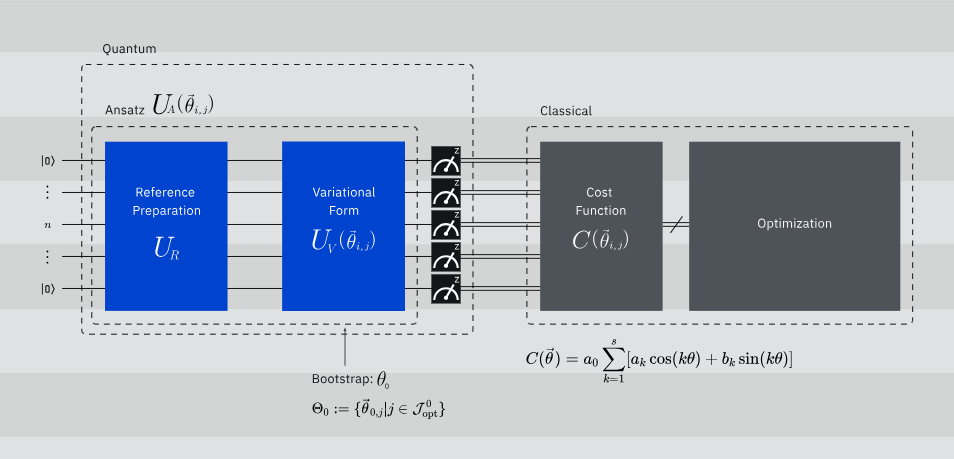
\includegraphics[width=1\linewidth]{Images/qsr_fig.png}
% \end{figure}
% The idea beind QSR is that the cost function $C(\theta)=\bra{\psi(\theta)}\hat{H}\ket{\psi(\theta)}$ can be expressed as a Fourier series in the following manner:
% \begin{align*}
% C(\vec{\theta})&=\bra{\psi(\theta)}\hat{H}\ket{\psi(\theta)}\\
% &=a_0+\sum_{k=1}^S [a_k \cos (k\theta)+b_k\sin(k\theta)]
% \end{align*}
% Depending on the periodicity and bandwidth of the original function, the set $S$ may be finite or infinite. For the purposes of the discussion, we will assume it is infinite. The next step is to sample the cost function $C(\theta)$ multiple times in order to obtain the Fourier coefficients $\{a_0,a_k,b_k\}_{k=1}^S$. Specifically, since we have $2S+1$ unknowns, we will need to sample the cost function $2S+1 $ times.

% If we then sample the cost function for $2S+1$ parameter values $\{\theta_1,\ldots,\theta_{2S+1}\}$, we can obtain the following system:
% \[
% \begin{pmatrix}
%     1 & \cos(\theta_1) & \sin(\theta_1) & \cos(2\theta_1) & \ldots & \sin (S\theta_1)\\
%     1 & \cos(\theta_2) & \sin(\theta_2) & \cos(2\theta_2) & \ldots &\sin(S\theta_2)\\
%     \vdots & \vdots & \vdots & \vdots & \ddots & \vdots \\
%     1 & \cos(\theta_{2S+1}) & \sin(\theta_{2S+1}) &\cos(2\theta_{2S+1}) & \ldots & \sin(S\theta_{2S+1})     
% \end{pmatrix}
% \begin{pmatrix} a_0 \\ a_1 \\ b_1 \\ a_2 \\ \vdots \\ b_s \end{pmatrix} =\begin{pmatrix} C(\theta_1)\\ C(\theta_2) \\ \vdots \\ C(\theta_{2S+1}) \end{pmatrix}
% \]
% that we'll rewrite as
% \[
% Fa=c
% \]
% In practice, this system is generally not consistent because the cost function values $c$ are not exact. Therefore, it is usually a good idea to normalized them by multiplying them by $F^{\dagger}$ on the left, which results in:
% \[
% F^{\dagger}Fa=F^{\dagger}c
% \]
% This new system is always consistent, and its solution is a least-squares solution to the original problem. If we have $k$ parameters instead of just one, and each parameter $\theta^i$ has its own $S_i$ for $i\in 1,\ldots,k$, then the total number of samples required is:
% \[
% T=\prod_{i=1}^k (2S_i+1)\leq \prod_{i=1}^k (2S_{max}+1)=(2S_{max}+1)^n 
% \]
% where $S_{max}=max_i(S_i)$. Furthermore, adjusting $S_{max}$ as a tunable parameter (instead of inferring it) opens up new possibilities, such as:
% \begin{itemize}
% \item \textbf{Oversampling}: to improve accuracy.
% \item \textbf{Undersampling}: to boost performance by reducing runtime overhead or eliminating local minima.
% \end{itemize}
% \subsubsection{QSR's Theoretical Layout}
% QSR's layout can be summarized as follows:
% \begin{itemize}
% \item Prepare reference operators $U_R$.
% \item We'll go from the state $\ket{0}$ to the reference state $\ket{\rho}$.
% \item Apply the variational form $U_V(\vec{\theta}_{i,j})$ to create an ansatz $U_A(\vec{\theta}_{i,j})$.
% \item Determine the bandwidth associated with each parameter in the ansatz. An upper bound is sufficient.
% \item Bootstrap at $i=0$ if we have a similar problem (typically found via classical simulation or sampling)
% \item Sample the cost function $C(\vec{\theta})=a_0+\sum_{k=1}^S [a_k \cos (k\theta)+bb_k \sin(k\theta)]$ at least $T$ times- $T=\prod_{i=1}^k (2S_i+1)\leq \prod_{i=1}^k (2S_{max}+1)=(2S_{max}+1)^n $
% \item Decide whether to oversample/undersample to balance speed vs accuracy by adjusting $T$.
% \item Compute the Fourier coefficients from the samples (i.e., solve the normalized linear system fo equations).
% \item Solve for the global minimum of the resulting regression function on a classical machine.
% \end{itemize}
% \subsection{Summary}
% With this lesson, you learned about multiple variational instances available:
% \begin{itemize}
%     \item General layout
%     \item Introducing weights and penalties to adjust a cost function.
%     \item Exploring undersampling vs oversampling to trade-off speed vs accuracy.
% \end{itemize}
% These ideas can be adapted to form a custom variational algorithm that fits your problem. We encourage you to share your results with the community. The next section we will explore how to use a variational algorithm to solve an application.

% \section{Variational Quantum Eigenlsolver}
% Usage Estimate: 73 minutes on ibm\_kyiv or 28 minutes on ibm\_manila. (NOTE:This is an estimate only. Your runtime may vary.)
% \subsection{Background}
% Variational quantum algorithms are promising candidate hybrid-quantum algorithms for observing quantum computational utility on noisy near-term devices. Variational algorithms are characterized by the use of classical optimization algorithm to iteratively update a parameterized trial solution, or ``ansatz". Chief among these methods is the Variational Quantum Eigensolver (VQE) that aims to solve for the ground state of a given Hamiltonian represented as a linear combination of Pauli terms, with an ansatz circuit where the number of parameters to optimize over is polynomial in number of qubits. Given that the size of the full solution vector is exponential in the number of qubits, successful minimization using VQE requires, in general, additional problem-specific information to define the structure of the ansatz circuit.

% Executing a VQE algorithm requires the following components:
% \begin{enumerate}
%     \item Hamiltonian and ansatz (problem specification)
%     \item Qiskit Runtime estimator
%     \item Classical Optimizer
% \end{enumerate}
% Although the Hamiltonian and ansatz require domain spcific knowledge to construct, these details are immaterial to the Runtime, and we execute a wide class of VQE problems in the same manner.

% \subsection{Requirements}
% Before starting this tutorial, ensure that you have the following installed:
% \begin{itemize}
%     \item Qiskit SDK 1.0 or later, with visualization support (pip install `qiskit[visulaization]'
%     \item Qiskit Runtime (pip install qiskit-ibm-runtime) 0.22 or later
%     \item SciPy(python -m pip install scipy)
% \end{itemize}
% \subsection{Setup}
% Here we import the tools needed for a VQE experiment.
% \begin{lstlisting}[language=Python]
% # General imports
% import numpy as np

% # Pre-defined ansatz circuit and operator class for Hamiltonian
% from qiskit.circuit.library import EfficientSU2
% from qiskit.quantum_info import SparsePauliOp

% # SciPy minimizer routine
% from scipy.optimize import minimize

% # Plotting functions
% import matplotlib.pyplot as plt
% \end{lstlisting}
% No output produced
% \begin{lstlisting}[language=Python]
% # runtime imports
% from qiskit_ibm_runtime import QiskitRuntimeService, Session
% from qiskit_ibm_runtime import EstimatorV2 as Estimator

% # To run on hardware, select the backend with the fewest number of jobs in the queue
% service = QiskitRuntimeService(channel="ibm_quantum")
% backend = service.least_busy(operational=True, simulator=False)
% \end{lstlisting}
% \subsubsection{Step1: Map classical inputs to a quantum problem}
% Although the problem instance in question for the VQE algorithm can come from a variety of domains, the form for execution through Qiskit Runtime is the same. Qiskit provides a convenience class for expressing hamiltonians in Pauli form, and a collection of widely used ansatz circuits in the qiskit.circuit.library.

% this example Hamiltonian is derived from a quantum chemistry problem.
% \begin{lstlisting}[language=Python]
% hamiltonian = SparsePauliOp.from_list(
%     [("YZ", 0.3980), ("ZI", -0.3980), ("ZZ", -0.0113), ("XX", 0.1810)]
% )
% \end{lstlisting}
% Our choice of ansatz is the EfficientSU2 that, by default, linearly entangles qubits, making it ideal for quantum hardware with limited connectivity.
% \begin{lstlisting}[language=Python]
% ansatz = EfficientSU2(hamiltonian.num_qubits)
% ansatz.decompose().draw("mpl", style="iqp")
% \end{lstlisting}
% Output:
% \begin{figure}[ht]
%     \centering
%     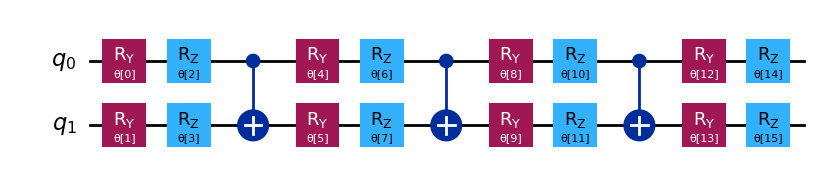
\includegraphics[width=0.75\linewidth]{Images/VQE_ansatz.png}
% \end{figure}

% From the previous figure we see that our ansatz circuit is defined by a vector of parameters, $\theta_i$, witht the total number given by:
% \begin{lstlisting}[language=Python]
% num_params = ansatz.num_parameters
% num_params
% \end{lstlisting}
% Output:
% \begin{lstlisting}
% 16
% \end{lstlisting}
% \subsubsection{Step2: Optimize problem for quantum execution}
% To reduce the total job execution time, Qiskit primitives only accept circuits (ansatz) and observables (Hamiltonian) that conform to the instructions and connectivity supported by the target system (referred to as instruction set architecutre (ISA)circuits and observables).

% \subsubsection{ISA circuit}
% Schedule a series of qiskit.transpiler passes to optimize the circuit for a selected backend and make it compatible with the backend's ISA. This can be easily done with a preset pass manager from qiskit.transpiler and its optimization\_level parameter.

% The lowest optimization level does the minimum needed to get the circuit running on the device; it maps the circuit qubits to the device qubits and ads swap gates to allow all two-qubit operations. The highest optimization level is much smarter and uses lots of tricks to reduce the overall gate count. Since multi-qubit gates have high error rates and qubits decohere over time, the shorter circuits shoudl give better results.

% \begin{lstlisting}[language=Python]
% from qiskit.transpiler.preset_passmanagers import generate_preset_pass_manager

% target = backend.target
% pm = generate_preset_pass_manager(target=target, optimization_level=3)

% ansatz_isa = pm.run(ansatz)
% \end{lstlisting}
% No Output produced
% \begin{lstlisting}
% ansatz_isa.draw(output="mpl", idle_wires=False, style="iqp")
% \end{lstlisting}
% Output:
% \begin{figure}[ht]
%     \centering
%     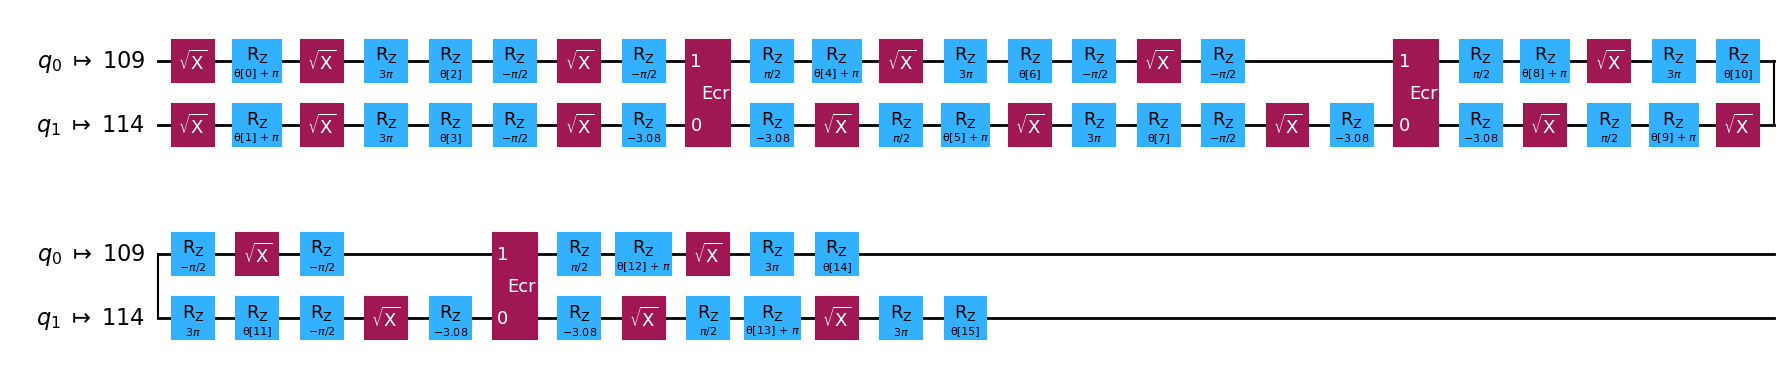
\includegraphics[width=0.75\linewidth]{Images/VQE_optimized_ansatz.png}
% \end{figure}

% \subsubsection{ISA observable}
% Transform the Hamiltonian to make it backend-compatible before running jobs with Runtime Esimtaor V2. Perform the transformation by using the apply\_layout metho of SparsePauliOp object.

% \begin{lstlisting}[language=Python]
% hamiltonian_isa = hamiltonian.apply_layout(layout=ansatz_isa.layout)
% \end{lstlisting}

% \subsubsection{Step 3: Execute using Qiskit Primitives}
% Like many classical optimization problems, the solution to a VQE problem can be formulated as a minimization of a scalar cost function. By definition, VQE looks to find the ground state solution to a Hamiltonian by optimizing the ansatz circuit parameters to minimize the expectation value (energy) of the Hamiltonian. With the Qiskit Runtime Estimator directly taking a Hamiltonian and parameterized ansatz, and returing the necessary energy, the cost function for a VQE isntance is quite simple.

% Note that run() method of Qiskit Runtime Estimator V2 takes an iterable fo primitve unified blocs (PUBs). Each PUB is an iterable in the format (circuit, observables, parameter\_values: Optional, precision: Optional)
% \begin{lstlisting}[language=Python]
% def cost_func(params, ansatz, hamiltonian, estimator):
%     """Return estimate of energy from estimator

%     Parameters:
%         params (ndarray): Array of ansatz parameters
%         ansatz (QuantumCircuit): Parameterized ansatz circuit
%         hamiltonian (SparsePauliOp): Operator representation of Hamiltonian
%         estimator (EstimatorV2): Estimator primitive instance
%         cost_history_dict: Dictionary for storing intermediate results

%     Returns:
%         float: Energy estimate
%     """
%     pub = (ansatz, [hamiltonian], [params])
%     result = estimator.run(pubs=[pub]).result()
%     energy = result[0].data.evs[0]

%     cost_history_dict["iters"] += 1
%     cost_history_dict["prev_vector"] = params
%     cost_history_dict["cost_history"].append(energy)
%     print(f"Iters. done: {cost_history_dict['iters']} [Current cost: {energy}]")

%     return energy
% \end{lstlisting}
% Note that, in addition to the array of optimization parameters that must be the first argument, we use additional arguments to pass the terms needed in the cost function, such as the cost\_history\_dict. This dictionary stores the current vector at each iteration, for example in case you need to restart the routine due to failure, and also returns the current iteration number and average time per iteration.
% \begin{lstlisting}[language=Python]
% cost_history_dict = {
%     "prev_vector": None,
%     "iters": 0,
%     "cost_history": [],
% }
% \end{lstlisting}
% We can now use a classical optimizer of our choice to minimize the cost function. Here, we use the COBYLA routine from SciPy through the minimize function. Note that when running on real quantum hardware, the choice of optimizer is important, as not all optimizers handle noisy cost function landscapes equally well. 

% To begin the routine, specify a random initial set of parameters:
% \begin{lstlisting}[language=Python]
% x0 = 2 * np.pi * np.random.random(num_params)
% \end{lstlisting}
% \begin{lstlisting}[language=Python]
% x0
% \end{lstlisting}
% Output:
% \begin{lstlisting}
% array([4.41731016, 3.07910816, 2.24090817, 4.49109315, 1.55032543,
%        3.80189756, 1.28634468, 2.38155768, 0.72212296, 3.15156603,
%        5.16945739, 3.10289414, 3.05826307, 0.24272269, 2.06257592,
%        5.23229471])
% \end{lstlisting}
% Because we are sending a large number of jobs that we would like to execute together, we use a Session to execute all the generated circuits in one block. Here args is the standard SciPy way to supply the additional parameters needed by the cost function.
% \begin{lstlisting}[language=Python]
% with Session(backend=backend) as session:
%     estimator = Estimator(session=session)
%     estimator.options.default_shots = 10000

%     res = minimize(
%         cost_func,
%         x0,
%         args=(ansatz_isa, hamiltonian_isa, estimator),
%         method="cobyla",
%     )
% \end{lstlisting}
% As the terminus of this routing we have a result in the standard SciPy OptimizeResult format. From this we see that it took nfev number of cost function evaluations to obtain the solution vector of parameter angles (x) that, when plugged into the ansatz circuit, yield the approximate ground state solution we were looking for.
% \begin{lstlisting}[language=Python]
% res
% \end{lstlisting}
% Output:
% \begin{lstlisting}
% message: Optimization terminated successfully.
%  success: True
%   status: 1
%      fun: -0.634701203143904
%        x: [ 2.581e+00  4.153e-01 ...  1.070e+00  3.123e+00]
%     nfev: 146
%    maxcv: 0.0
% \end{lstlisting}
% \subsubsection{Step 4: Post-process, return result in classical format}
% If the procedure terminates correctly, then the prev\_vector and iters values in our cost\_history\_dict dictionary should be equal to the solution vector and total number of function evaluation, respectively. This is easy to verify:
% \begin{lstlisting}[language=Python]
% all(cost_history_dict["prev_vector"] == res.x)
% \end{lstlisting}
% Output:
% \begin{lstlisting}
% False
% \end{lstlisting}
% We can also now view the progress toward convergence as monitored by the cost history at each iteration:
% \begin{lstlisting}[language=Python]
% fig, ax = plt.subplots()
% ax.plot(range(cost_history_dict["iters"]), cost_history_dict["cost_history"])
% ax.set_xlabel("Iterations")
% ax.set_ylabel("Cost")
% plt.draw()
% \end{lstlisting}
% Output:
% \begin{figure}
%     \centering
%     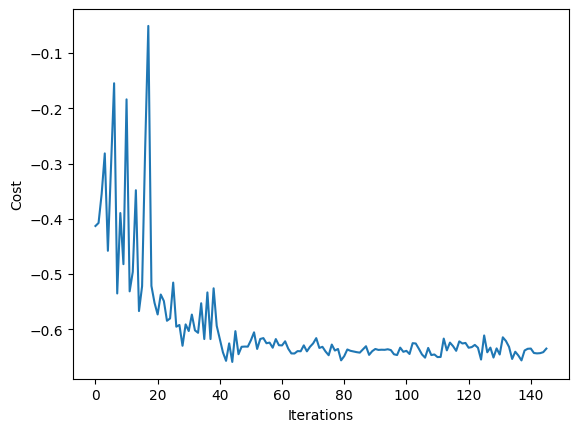
\includegraphics[width=0.75\linewidth]{Images/VQE_results.png}
% \end{figure}
% \begin{lstlisting}[language=Python]
% import qiskit_ibm_runtime

% qiskit_ibm_runtime.version.get_version_info()
% \end{lstlisting}
% Output:
% \begin{lstlisting}
% '0.28.0'    
% \end{lstlisting}

% \begin{lstlisting}[language=Python]
% import qiskit

% qiskit.version.get_version_info()
% \end{lstlisting}
% Output:
% \begin{lstlisting}
% '1.2.0'    
% \end{lstlisting}


% % \chapter{Sample-based quantum diagonalization (SQD) Algorithm}
% % We show how to post-process noisy quantum samples to find an approximation to the ground state of the nitrogen molecule $N_2$ at equilibrium bond length, using the sample-based quantum diagonalization (SQD) algorithm, for samples taken from a 36-qubit quantum circuit (32 system qubits + 4ancilla qubits). A Qiskit based implementation is available as a Qiskit Addons, more details can be found in the corresponding docs with a simple example to get started. SQF is a technique for finding eigenvalue s and eigenvectors of quantum operators, such as a quantum system Hamiltonian, using quantum and distributed classical computing together. Classical distributed computing is used to process samples obtained from a quantum processor, and to project and diagonalize a target Hamiltonian in a subspace spanned by them. This allows SQF to be robust to samples corrupted by quantum noised ad deal with large Hamiltonians such as chemistry Hamiltonian with millions of interaction terms, beyond the reach of any exact diaonilaztion method. An SQD workflow has the following steps:
% % \begin{enumerate}
% %     \item Choose a circuit ansatz and apply it on a quantum computer to a reference state (in this case, the hatree-Fock state).
% %     \item Sample bitstrings from the resulting quantum state
% %     \item Run the self consistent configuration recovery procedure on the bitstrings to obtain the approximation to the ground state.
% % \end{enumerate}

% % \section{Quantum Chemistry}
% % The properties of molecules are largely determined by the structure of the electrons within them. As fermionic particles, electrons can be described using a mathematical formalism called second quantization. The idea is that there are a number of orbitals, each of which can be either empty or occupied by a fermion. A system of N orbitals is described by a set of fermionic annihilation operators $\{\hat{a}_p\}_{p=1}^N$ that satisfy the fermionic anti-commutation relations,
% % \[
% % \hat{a}_p\hat{a}_q + \hat{a}_q \hat{a}_p=0
% % \]
% % \[
% % \hat{a}_p\hat{a}_q^{\dagger} + \hat{a}_q^{\dagger}\hat{a}_p = \delta_{pq}
% % \]
% % The adjoint $\hat{a}_p^{\dagger}$ is called a creation operator.

% % So far, our exposition has not accounted for spin, which is a fundamental property of fermions. When accounting for spin, the orbitals come in pairs called spatial orbitals. each spatial orbitals is composed of two spin orbitals, one that is labeled ``spin-$\alpha$" and one that is labeled ``spin-$\beta$". We then write $\hat{a}_{p\sigma}$ for the annhilation operator associated with the spin orbital with spin $\sigma$($\sigma \in \{\alpha,\beta\}$) in spatial orbital $p$. If we take $N$ to be the number of spatial orbitals., then there are a total of $2N$ spin-orbitals. The Hilbert space of this system is spanned by $2^{2N}$ orthonormal basis vectors labeled with two-part bitstrings $\ket{z}=\ket{z_{\beta}\ket{z_{\alpha}\alpha \ket{z_{\beta,N}\ldotsz-[\beta,1}\z_{\alpha_N,1}\ldots z-{\alpha,1}$

